% Copyright (C) 2010,2012,2013,2014 The ESPResSo project
% Copyright (C) 2002,2003,2004,2005,2006,2007,2008,2009,2010 
%   Max-Planck-Institute for Polymer Research, Theory Group
%  
% This file is part of ESPResSo.
%   
% ESPResSo is free software: you can redistribute it and/or modify it
% under the terms of the GNU General Public License as published by the
% Free Software Foundation, either version 3 of the License, or (at your
% option) any later version.
%  
% ESPResSo is distributed in the hope that it will be useful, but
% WITHOUT ANY WARRANTY; without even the implied warranty of
% MERCHANTABILITY or FITNESS FOR A PARTICULAR PURPOSE.  See the GNU
% General Public License for more details.
%  
% You should have received a copy of the GNU General Public License
% along with this program.  If not, see <http://www.gnu.org/licenses/>.
%
\chapter{\es{} quick reference}
\label{chap:quickref}

\index{quick reference of Tcl-commands}

\setcounter{essyntaxcounter}{0}
% Redefine the layout commands
\renewenvironment{essyntax}{%
  \stepcounter{essyntaxcounter}%
  \par\noindent%
  \makebox[0pt][l]{\rule[0.8\baselineskip]{\linewidth}{1pt}}
  \hspace{3em}%
  \begin{minipage}[t]{\linewidth-5em}%
    \setlength{\parindent}{-3em}%
    \ttfamily
  }{%
  \end{minipage}%
  \hfill{\small\pageref{essyntax:\arabic{essyntaxcounter}}}
}
\renewcommand{\variant}[1]{\par}

% Now input the file
\chapter{\es{} quick reference}
\label{chap:quickref}

\index{quick reference of Tcl-commands}
%\documentclass[
a4paper,                        % paper size
11pt,                           % font size
twoside,                        % two sided
footsepline,                    % add a line to separate the footer
headsepline,                    % add a line to separate the header
headexclude,                    % header does not belong to the text
footexclude,                    % footer does not belong to the text
pagesize,                       % set the pagesize in a DVI document
bibtotocnumbered,               % add the bibliography to the TOC
idxtotoc                        % add the index to the TOC
%openright,                      % start a new chapter on the right page
%,DIV12
%,draft
]{scrreprt}

\usepackage[draft]{varioref}    % defines \vref
\usepackage{hyperref}                      % automatically creates links when
                                % using pdflatex, defines \url
\usepackage{ifpdf}              % defines \ifpdf
\usepackage{graphicx}           % handles graphics
\usepackage{makeidx}            % creates the index
\usepackage{color}              % use colors

\usepackage{amsmath}

\usepackage{verbatim}           % required for \verbatim and \endverbatim
\usepackage{fancyvrb}
\usepackage{tocloft}            % required for the quickref
\usepackage{calc}               % compute length
\usepackage{ifthen}             % provide ifthen
\usepackage{xspace}
\usepackage{units}
\usepackage[numbers]{natbib}

% Make '_' a normal character (from http://www.tug.org/TeXnik/mainFAQ.cgi)
\usepackage{underscore}
% \begingroup
%   \lccode`\~=`\_
% \lowercase{\endgroup
%   \pdfstringdefDisableCommands{\let~\relax}%
% }
%%%%%%%%%%%%%%%%%%%%%%%%%%%%%%%%%%%%%%%%%%%%%%%%%%
%%%%%%%%%%%%%%%%%%%%%%%%%%%%%%%%%%%%%%%%%%%%%%%%%%
%%%%%%%%% New Commands and Environments %%%%%%%%%%
%%%%%%%%%%%%%%%%%%%%%%%%%%%%%%%%%%%%%%%%%%%%%%%%%%
%%%%%%%%%%%%%%%%%%%%%%%%%%%%%%%%%%%%%%%%%%%%%%%%%%
\newcommand{\es}{\mbox{\textsf{ESPResSo}}\xspace}
\newcommand{\ie}{\textit{i.e.}\xspace}
\newcommand{\eg}{\textit{e.g.}\xspace}
\newcommand{\etal}{\textit{et al.}\xspace}

\newcommand{\codebox}[1]%
{\texttt{#1}}

\DefineVerbatimEnvironment{code}{Verbatim}%
{commandchars=\\\{\}}
\makeatletter
\newenvironment{tclcode}
{%
  \addtolength{\linewidth}{-2em}% set the line length
  \@minipagetrue%%%DPC%%%
  \@tempswatrue%%%DPC%%%
  \hsize=\linewidth%
  \setbox0=\vbox\bgroup\verbatim
}{\endverbatim
  \unskip\setbox0=\lastbox%%%DPC%%%
  \egroup
  \par%
  \noindent\hspace{1em}%
  \codebox{\box0}%
  \par\noindent%
}
\makeatother

% required so that we can set index numbers bold
% \index{Some example|mainindex}
\newcommand*{\mainindex}[1]{\textbf{\hyperpage{#1}}}

\newcommand{\todo}[1]{
  \marginpar{%
    \setlength{\fboxrule}{1pt}
    \fcolorbox[gray]{0}{0.9}{%
      \parbox{\marginparwidth-2\fboxrule-2\fboxsep}{%
        \bf\raggedright\scriptsize #1%
      }%
    }%
  }%
}

\makeatletter
\renewcommand{\minisec}[1]{\@afterindentfalse \vskip 1.5ex
  {\parindent \z@
    \raggedsection\normalfont\sffamily\itshape\nobreak#1\par\nobreak}%
  \@afterheading}
\makeatother

%%%%%%%%%%%%%% Syntax Description %%%%%%%%%%%%%%%

%%%%%% SYNTAX DEFINITION LAYOUT
%% Defines environments and commands to be used when defining the
%% syntax of a Tcl command.
% typesetting inside a command definition
% keywords/literals
\newcommand{\lit}[1]{\mbox{\texttt{#1}}}
\newcommand{\keyword}[1]{\mbox{\texttt{#1}}}
% variables
\newcommand{\var}[1]{\ensuremath{\mathrm{\mathit{#1}}}}
% option
\newcommand{\opt}[1]{\mbox{\textrm{[}#1\textrm{]}}}
\newcommand{\optlong}[1]{\textrm{[}#1\textrm{]}}
% alternatives
\newcommand{\alt}[1]{\textrm{(} #1 \textrm{)}}
\newcommand{\asep}{$|$\xspace}
% variant
% \rawvariant is required, as the command is changed during the
% essyntax environment
\newcommand{\rawvariant}[1]{\mbox{\textnormal{(#1)}}\xspace}
\newcommand{\variant}[1]{\rawvariant{#1}}
\newcommand{\fmark}[1]{%
  \raisebox{1ex}{%
    \textrm{\footnotesize #1}%
  }%
}
% feature
\newcommand{\feature}[1]{\texttt{\MakeUppercase{#1}}}

\newcommand{\require}[2]{%
  \mbox{#2\,\fmark{#1}}%
}
\newcommand{\required}[2][]{%
  \ifthenelse{\equal{#1}{}}{#2}{%
    \mbox{\fmark{#1}\,\feature{#2}}%
  }
}
\newenvironment{features}{%
  \par\smallskip%
  \small%
  \textrm{Required\hspace{1ex}features:}%
  \raggedright%
}{}

%% Layout thesyntax description box
\newsavebox{\theessyntaxbox}
\newlength{\essyntaxboxheight}
\newlength{\essyntaxboxdepth}
\newenvironment{essyntaxbox}{%
  \par\noindent%
 \begin{lrbox}{\theessyntaxbox}%
   \begin{minipage}{\linewidth-5em}%
     \ttfamily%
     \setlength{\parindent}{-3em}%
   }{%
   \end{minipage}%
 \end{lrbox}%
 \settoheight{\essyntaxboxheight}{\usebox{\theessyntaxbox}}%
 \settodepth{\essyntaxboxdepth}{\usebox{\theessyntaxbox}}%
 \hspace{1.5em}%
 \rule[-\essyntaxboxdepth]{1pt}{\essyntaxboxheight+\essyntaxboxdepth}%
 \hspace{3.5em}%
 \usebox{\theessyntaxbox}%
}

%% Environment for syntax descriptions
\newcounter{essyntaxcounter}
\setcounter{essyntaxcounter}{0}
\newenvironment{essyntax}{%
  \stepcounter{essyntaxcounter}%
  \label{essyntax:\arabic{essyntaxcounter}}
  % Create headings
  \minisec{Syntax}\nopagebreak%
  \smallskip\nopagebreak%
  \renewcommand{\variant}[1]{\par\rawvariant{##1}}
  \begin{essyntaxbox}%
  }{%
  \end{essyntaxbox}%
  \renewcommand{\variant}[1]{\rawvariant{##1}}
  \minisec{Description}%
}
% Define the starred environment (identical to unstarred, only it is
% not copied to the Quick reference)
\newenvironment{essyntax*}{\essyntax}{\endessyntax}

%% List-environment for the description of the arguments of a command
\newenvironment{arguments}{
  \minisec{Arguments}
  \begin{list}{}{
      \setlength{\rightmargin}{1em}
      \setlength{\leftmargin}{2em}
      \setlength{\partopsep}{0pt}
      \setlength{\topsep}{1ex}
      \setlength{\parsep}{0.5ex}
      \setlength{\listparindent}{-1em}
      \setlength{\labelwidth}{0.5em}
      \setlength{\labelsep}{0.5em}
      \renewcommand{\makelabel}[1]{\textbullet\,\texttt{##1}}
    }
  }{
  \end{list}
}

%%%%%%%%%%%%%%%%%%%%%%%%%%%%%%%%%%%%%%%%%%%%%%%%%%
%%% Declare new features/commands/analyze subcommands
%%%%%%%%%%%%%%%%%%%%%%%%%%%%%%%%%%%%%%%%%%%%%%%%%%
% Feature declaration
\newcommand{\newfeature}[1]{%
  \index{features!#1|mainindex}%
  \hypertarget{#1}{\texttt{\textbf{#1}}}%
}

% Create label and index entries for an Espresso tcl command
\newcommand{\newescommand}[2][NONE]{%
  \ifthenelse{\equal{#1}{NONE}}%
  {\label{tcl:#2}}%
  {\label{tcl:#1}}%
  \index{#2@\texttt{#2} (Tcl-command)|mainindex}%
  \index{Tcl-commands!#2@\texttt{#2}|mainindex}%
}

% Create index entries for analysis functions
\newcommand{\analyzeindex}[1]{%
  \index{#1|mainindex}%
  \index{analysis!#1|mainindex}%
}

%%%%%%%%%%%%%%%%%%%%%%%%%%%%%%%%%%%%%%%%%%%%%%%%%%
%%%%%%%%%%%%%%%%%%%%%%%%%%%%%%%%%%%%%%%%%%%%%%%%%%
%%%%%%%%%%%%%%%% Other Settings %%%%%%%%%%%%%%%%%%
%%%%%%%%%%%%%%%%%%%%%%%%%%%%%%%%%%%%%%%%%%%%%%%%%%
%%%%%%%%%%%%%%%%%%%%%%%%%%%%%%%%%%%%%%%%%%%%%%%%%%
\makeindex

%%%%%%%%%%%%%%%%%%%%%%%%%%%%%%%%%%%%%%%%%%%%%%%%%%
%%%%%%%%%%%%%%%%%%%%%%%%%%%%%%%%%%%%%%%%%%%%%%%%%%
%%%%%%%%%%%%%%%%% Main Document %%%%%%%%%%%%%%%%%%
%%%%%%%%%%%%%%%%%%%%%%%%%%%%%%%%%%%%%%%%%%%%%%%%%%
%%%%%%%%%%%%%%%%%%%%%%%%%%%%%%%%%%%%%%%%%%%%%%%%%%
\begin{document}
\titlehead{
  \begin{center}
    \includegraphics[width=5cm]{figures/logo}
  \end{center}
}
%\subject{}
\title{\es{} User's Guide}
%\author{}
%\date{\today}
\maketitle

\pdfbookmark{Contents}{toc}
\tableofcontents

\chapter{Introduction}
\label{chap:intro}

(new)

\begin{itemize}
\item \es{} is a generic soft matter simulation packages
\item for molecular dynamics simulations in soft matter research
\item focussed on coarse-grained models
\item employs modern algorithms (Lattice-Boltzmann, DPD, P3M, \ldots)
\item written in C for maximal portability
\item Tcl-controlled
\item parallelized
\end{itemize}

\section{Guiding principles}
\label{sec:ideas}

(from paper: 2.1 Goals and principles)

\es
\begin{itemize}
\item does \emph{not} do the physics for you!
\item requires you to understand what you do (can not be used as a
  black box)
\item gives you maximal freedom (flexibility)
\item is extensible
\item integrates system setup, simulation and analysis, as this can't
  be strictly separated in soft matter simulations
\item has no predefined units
\item sets as few defaults as possible
\end{itemize}

\section{Algorithms contained in \es}

The following algorithms are implemented in \es{}:

\begin{itemize}
\item ensembles: NVE, NVT, NpT
\item charged systems:
  \begin{itemize}
  \item P3M for fully periodic systems
  \item ELC and MMM-family of algorithms for charged systems with
    non-periodic boundary conditions
  \item Maggs algorithm 
  \end{itemize}
\item Hydrodynamics:
  \begin{itemize}
  \item DPD (as a thermostat)
  \item Lattice-Boltzmann
  \end{itemize}
\end{itemize}

\section{Basic program structure}
\label{sec:structure}

(from paper: 2.2 Basic program structure)

\begin{itemize}
\item Control level: \texttt{Tcl}
\item ``Kernel'' written in \texttt{C}
\item This user's guide will focus on the control level
\end{itemize}

\section{On units}
\label{sec:units}
\index{units}
\index{length unit}
\index{time unit}
\index{energy unit}
\index{physical units}

What is probably one of the most confusing subjects for beginners of
\es is, that \es does not predefine any units.  While most MD programs
specify a set of units, like, for example, that all lengths are
measured in \AA ngstr\"om or nanometers, times are measured in nano- or
picoseconds and energies are measured in $\frac{kJ}{\mathrm{mol}}$,
\es does not do so.

Instead, the length-, time- and energy scales can be freely chosen by
the user.  A length of $1.0$ can mean a nanometer, an \AA ngstr\"om,
or a kilometer - depending on the physical system, that the user has
in mind when he writes his \es-script.  The user can choose the unit
system that suits the system best.

When creating particles that are intended to represent a specific type
of atoms, one will probably use a length scale of \AA ngstr\"om.  This
would mean, that \eg the parameter $\sigma$ of the Lennard-Jones
interaction between two atoms would be set to twice the van-der-Waals
radius of the atom in \AA ngstr\"om.  Alternatively, one could set
$\sigma$ to $2.0$ and measure all lengths in multiples of the
van-der-Waals radius.

The second choice to be made is the energy (and time-) scale.  One can
for example choose to set the Lennard-Jones parameter $\epsilon$ to
the energy in $\frac{kJ}{\mathrm{mol}}$.  Then all energies will be
measured in that unit.  Alternatively, one can choose to set it to
$1.0$ and measure everything in multiples of the van-der-Waals binding
energy.

As long as one remains within the same unit system throughout the
whole \es-script, there should be no problems.

\section{Requirements}
\label{sec:requirements}
\index{requirements}

The following libraries and tools are required to be able to compile
and use \es:

\begin{description}
\item[Tcl/Tk] \index{Tcl/Tk} \es{} requires the Toolkit Command
  Language Tcl/Tk \footnote{\url{http://www.tcl.tk/}} in the version
  8.3 or later.  Some example scripts will only work with Tcl 8.4. You
  do not only need the interpreter, but also the header files and
  libraries.  Depending on the operating system, these may come in
  separate development packages. If you want to use a graphical user
  interface (GUI) for your simulation scripts, you will also need Tk.
  
\item[FFTW] \index{FFTW} In addition, \es{} needs the FFTW library
  \footnote{\url{http://www.fftw.org/}} for Fourier transforms.
  ESPResSo can work with both the 2.1.x and 3.0.x series. Again, the
  header files are required.
  
\item[MPI] \index{MPI} Finally, if you want to use \es{} in parallel,
  you need a working MPI environment (version 1.2). Currently, the
  following MPI implementations are supported:
  \begin{itemize}
  \item LAM/MPI is the preferred variant
  \item MPICH, which seems to be considerably slower than LAM/MPI in
    our benchmarks.
  \item On AIX systems, \es{} can also use the native POE parallel
    environment.
  \item On DEC/Compaq/HP OSF/Tru64, \es{} can also use the native
    dmpirun MPI environment.
  \end{itemize}
\end{description}


\section{Syntax description}
\label{sec:syntax}


Throughout the user's guide, formal definitions of the syntax of
several Tcl-commands can be found. The following conventions are used
in these decriptions:
\begin{itemize}
\item Different \emph{variants} of a command are labelled \variant{1},
  \variant{2}, \ldots
\item Keywords and literals of the command that have to be typed
  exactly as given are written in \lit{typewriter} font.
\item If the command has variable arguments, they are set in
  \var{italic font}. The description following the syntax definition
  should contain a detailed explanation of the argument and its
  type.
\item \texttt{\alt{\var{alt1} \asep \var{alt2}}} specifies, that one
  of the alternatives \var{alt1} or \var{alt2} can be used.
\item \texttt{\opt{\var{argument}}} specifies, that the arugment
  \var{argument} is optional, \ie{} it can be omitted.
\item When an optional argument or a whole command is marked by a
  superscript label (\fmark{1}), this denotes that the argument can
  only be used, when the corresponding feature (see appendix
  \vref{chap:features}) specified in ``Required features'' is
  activated.
\end{itemize}


\minisec{Example}

\renewcommand{\variant}[1]{\par\rawvariant{#1}}
\begin{essyntaxbox}
  \variant{1} 
  constraint wall normal \var{n_x} \var{n_y} \var{n_z} 
  dist \var{d} type \var{id}
  
  \variant{2}
  constraint sphere center \var{c_x} \var{c_y} \var{c_z} 
  radius \var{rad} direction \var{direction} type \var{id} 
  
  \require{1}{%
    \variant{3}
    constraint rod center \var{c_x} \var{c_y} 
    lambda \var{lambda}
  } 
  
  \require{2,3}{%
    \variant{4}
    constraint ext_magn_field \var{f_x} \var{f_y} \var{f_z} 
  }

  \begin{features}
    \required{CONSTRAINTS}
    \required[1]{ELECTROSTATICS}
    \required[2]{ROTATION}
    \required[3]{DIPOLES}
  \end{features}

\end{essyntaxbox}
\renewcommand{\variant}[1]{\rawvariant{#1}}

%%% Local Variables: 
%%% mode: latex
%%% TeX-master: "ug"
%%% End: 


\chapter{First steps}
\label{chap:firststeps}

\section{Quick installation}

\index{configure}\index{make}

If you have the requirements (see section \vref{sec:requirements})
installed, in many cases, to compile \es{}, it is enough to execute
the following sequence of two steps in the directory where you have
unpacked the sources:
\begin{code}
configure
make
\end{code}

\todo{Mention minimal configuration without myconfig.h}
In some cases, \eg{} when \es{} needs to be compiled for several
different platforms or when different versions with different sets of
features are required, it might be useful to execute the commands not
in the source directory itself, but to start \texttt{configure} from
another directory (see section \vref{sec:builddir}). Furthermore, many
features of \es{} can be selectively turned on or off in the local
configuration header of \es{} (see section \vref{sec:myconfig}) before
starting the compilation with \texttt{make}.

The shell script \texttt{configure} prepares the source code for
compilation. It will determine how to use and where to find the
different libraries and tools required by the compilation process, and
it will test what compiler flags are to be used.  The script will find
out most of these things automatically.  If something is missing, it
will complain and give hints how to solve the problem.  The
configuration process can be controlled with the help of a number of
options that are explained in section \vref{sec:configure}.

The command \texttt{make} will compile the source code. Depending on
the options passed to the program, \texttt{make} can also be used for
a number of other things:
\begin{itemize}
\item It can install and uninstall the program to some other
  directories. However, normally it is not necessary to actually
  \textit{install} \es{} to run it.
\item It can test the \es{} program for correctness.
\item It can build the documentation.
\end{itemize}
The details of the usage of \texttt{make} are described in section
\vref{sec:make}.

When these steps have successfully completed, \es{} can be started
with the command (see section \vref{sec:run})
\begin{code}
Espresso
\end{code}

\section{Running \es}

\footnote{\url{http://www.tcl.tk/man/tcl8.5/tutorial/tcltutorial.html}}

\es{} is implemented as an extension to the Tcl script language. This means that you need to write a
script for any task you want to perform with \es. To learn about the Tcl script language and
especially the \es{} extensions, this chapter offers two tutorial scripts. The first will guide you
step by step through creating your first simulation script, while the second script is a well
documented example simulation script. Since the latter is slightly more complex and uses more
advanced features of \es{}, we recommend to work through both scripts in the presented order.

\section{Creating the first simulation script}

This section introduces some of the features of \es\ by
constructing step by step a simulation script for a simple salt crystal.
We cannot give a full Tcl tutorial here; however, most of the constructs
should be self--explanatory. We also assume that the reader is familiar with the
basic concepts of a MD simulation here. The code pieces can be copied step by
step into a file, which then can be run using \verb|Espresso <file>| from the
\es source directory.

Our script starts with setting up the initial configuration.  Most conveniently,
one would like to specify the density and the number of particles of the system
as parameters:
\begin{tclcode}
set n_part 200; set density 0.7
set box_l [expr pow($n_part/$density,1./3.)]
\end{tclcode}
These variables do not change anything in the simulation engine, but are just
standard Tcl variables; they are used to increase the readability and
flexibility of the script. The box length is not a parameter of this simulation;
it is calculated from the number of particles and the system density. This
allows to change the parameters later easily, e.~g.\ to simulate a bigger
system.

The parameters of the simulation engine are modified by the \verb|setmd|
command. For example
\begin{tclcode}
setmd box_l $box_l $box_l $box_l
setmd periodic 1 1 1
\end{tclcode}
defines a cubic simulation box of size \verb|box_l|, and periodic boundary
conditions in all spatial dimensions. We now fill this simulation box with
particles
\begin{tclcode}
set q 1; set type 0
for {set i 0} { $i < $n_part } {incr i} {
  set posx [expr $box_l*[t_random]]
  set posy [expr $box_l*[t_random]]
  set posz [expr $box_l*[t_random]]
  set q [expr -$q]; set type [expr 1-$type]
  part $i pos $posx $posy $posz q $q type $type 
}
\end{tclcode}
This loop adds \verb|n_part| particles at random positions, one by one.  In this
construct, only two commands are not standard Tcl commands: the random
number generator \verb|t_random| and the \verb|part| command, which is used to
specify particle properties, here the position, the charge \verb|q| and the
type. In \es\ the particle type is just an integer number which allows to group
particles; it does not imply any physical parameters. Here we use it to tag the
charges: positive charges have type 0, negative charges have type 1.

Now we define the ensemble that we will be simulating. This is done using the
\verb|thermostat| command. We also set some integration scheme parameters:
\begin{tclcode}
setmd time_step 0.01; setmd skin 0.4
set temp 1; set gamma 1
thermostat langevin $temp $gamma
\end{tclcode}
This switches on the Langevin thermostat for the NVT ensemble, with temperature
\verb|temp| and friction \verb|gamma|. The skin depth \verb|skin| is a parameter
for the link--cell system which tunes its performance, but cannot be discussed
here.

Before we can really start the simulation, we have to specify the
interactions between our particles.  We use a simple, purely repulsive
Lennard-Jones interaction to model the hard core repulsion
\citep{grest86a}, and the charges interact via the Coulomb potential:
\begin{tclcode}
set sig 1.0; set cut   [expr 1.12246*$sig]
set eps 1.0; set shift [expr 0.25*$eps]
inter 0 0 lennard-jones $eps $sig $cut $shift 0
inter 1 0 lennard-jones $eps $sig $cut $shift 0
inter 1 1 lennard-jones $eps $sig $cut $shift 0
inter coulomb 10.0 p3m tunev2 accuracy 1e-3 mesh 32
\end{tclcode}
The first three \verb|inter| commands instruct \es\ to use the same purely
repulsive Lennard--Jones potential for the interaction between all combinations
of the two particle types 0 and 1; by using different parameters for different
combinations, one could simulate differently sized particles.  The last line sets
the Bjerrum length to the value 10, and then
instructs \es\ to use P$^3$M for the Coulombic interaction and to try to find
suitable parameters for an rms force error below $10^{-3}$, with a fixed mesh
size of 32. The mesh is fixed here to speed up the tuning; for a real
simulation, one will also tune this parameter.

If we want to calculate the temperature of our system from the kinetic energy,
we need to know the number of the degrees of freedom of the particles.
In \es\ these are usually 3 translational plus 3 rotational degrees of freedom
(if ROTATION is compiled into the code). You can get this number
in the following way \footnote{Note: there also exists a predefined tcl function {\it degrees_of_freedom} which does the same.}:

\begin{tclcode}
   if { [regexp "ROTATION" [code_info]] } { 
     set deg_free 6
   } else { set deg_free 3 }
\end{tclcode}

Now we can integrate the system:
\begin{tclcode}
set integ_steps 200
for {set i 0} { $i < 20 } { incr i} {
  set temp [expr [analyze energy kinetic]/($deg_free/2.0)*$n_part)]
  puts "t=[setmd time] E=[analyze energy total], T=$temp"
  integrate $integ_steps 
}
\end{tclcode}
This code block is the primary simulation loop and runs
$20\times$\verb|integ_steps| MD steps. Every \verb|integ_steps| time steps, the
potential, electrostatic and kinetic energies are printed out (the latter one as
temperature). However, the simulation will crash: \es\ complains about particle
coordinates being out of range. The reason for this is simple: Due to the
initial random setup, the overlap energy is around a million kT, which we first
have to remove from the system. In \es, this is can be accelerated by capping
the forces, i.~e.\ modifying the Lennard--Jones force such that it is constant
below a certain distance. Before the integration loop, we therefore insert this
equilibration loop:
\begin{tclcode}
for {set cap 20} {$cap < 200} {incr cap 20} {
  puts "t=[setmd time] E=[analyze energy total]"
  inter ljforcecap $cap; integrate $integ_steps 
}
inter ljforcecap 0
\end{tclcode}
This loop integrates the system with a force cap of initially 20 and finally
200.  The last command switches the force cap off again. With this
equilibration, the simulation script runs fine.

However, it takes some time to simulate the system, and one will probably like
to write out simulation data to configuration files, for later analysis. For
this purpose \es\ has commands to write simulation data to a Tcl stream
in an easily parsable form.  We add the following lines at end of integration
loop to write the configuration files ``config\_0'' through ``config\_19'':
\begin{tclcode}
set f [open "config_$i" "w"]
blockfile $f write tclvariable {box_l density}
blockfile $f write variable box_l
blockfile $f write particles {id pos type}
close $f
\end{tclcode}
The created files ``config\_...'' are human--readable and look like
\begin{tclcode}
{tclvariable
        {box_l 10}
        {density 0.7}
}
{variable  {box_l 10.0 10.0 10.0} }
{particles {id pos type}
        {0 3.51770181433 4.3208975936 5.30529948918 0}
        {1 3.93145531704 6.58506447035 6.95045147034 1}
        ...
}
\end{tclcode}
As you can see, such a \emph{blockfile} consists of several Tcl lists,
which are called \emph{blocks}, and can store any data available from the
simulation. Reading a configuration is done by the following simple script:
\begin{tclcode}
set f [open $filename "r"]
while { [blockfile $f read auto] != "eof" } {}
close $f
\end{tclcode}
The \verb|blockfile read auto| commands will set the Tcl variables \verb|box_l|
and \verb|density| to the values specified in the file when encountering the
\verb|tclvariable| block, and set the box dimensions for the simulation when
encountering the \verb|variable| block. The particle positions and types of all
216 particles are restored when the \verb|particles| block is read. Note that it
is important to have the box dimensions set before reading the particles, to
avoid problems with the periodic boundary conditions.

\begin{figure}[tb]
  \centering
  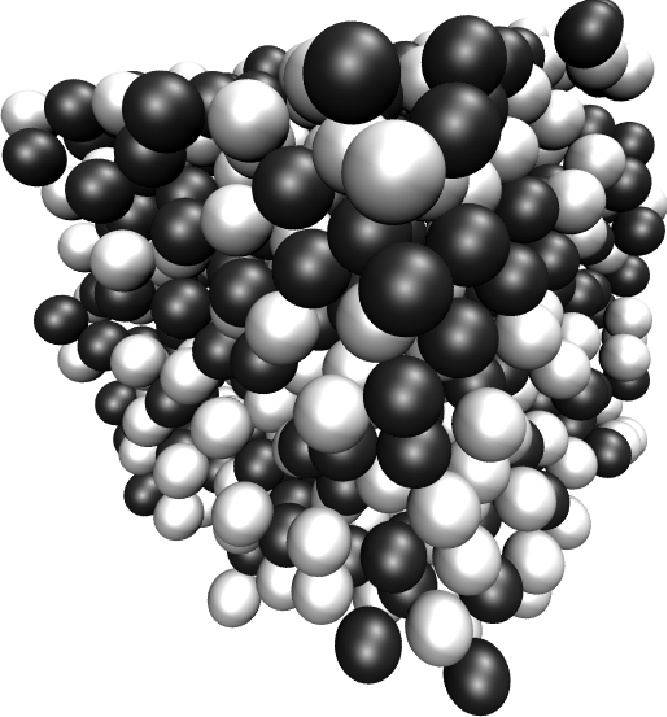
\includegraphics[width=0.4\textwidth]{figures/salt.png}
  \caption{VMD Snapshot of the salt system}
  \label{fig:snapshot}
\end{figure}

With these configurations, we can now investigate the system. As an example, we
will create a second script which calculates the averaged radial distribution
functions $g_{++}(r)$ and $g_{+-}(r)$. The radial distribution function for a
the current configuration can be obtained using the \verb|analyze| command:
\begin{tclcode}
set rdf [analyze rdf 0 1 0.9 [expr $box_l/2] 100]
set rlist ""
set rdflist ""
foreach value [lindex $rdf 1] {
  lappend rlist   [lindex $value 0]
  lappend rdflist [lindex $value 1] 
}
\end{tclcode}
The shown \verb|analyze rdf| command returns the distribution function of
particles of type 1 around particles of type 0 (i.~e.\ of opposite charges) for
radii between $0.9$ and half the box length, subdivided into $100$ bins.
Changing the first two parameters to either ``0 0'' or ``1 1'' allows to
determine the distribution for equal charges. The result is a list of $r$ and
$g(r)$ pairs, which the following foreach loop divides up onto two lists
\verb|rlist| and \verb|rdflist|.

To average over a set of configurations, we put the two last code snippets into
a loop like this:
\begin{tclcode}
set cnt 0
for {set i 0} {$i < 100} {incr i} { lappend avg_rdf 0}
foreach filename $argv {
  set f [open $filename "r"]
  while { [blockfile $f read auto] != "eof" } {}
  close $f
  set rdf [analyze rdf 0 1 0.9 [expr $box_l/2] 100]
  set rlist ""
  set rdflist ""
  foreach value [lindex $rdf 1] {
     lappend rlist   [lindex $value 0]
     lappend rdflist [lindex $value 1] }
  set avg_rdf [vecadd $avg_rdf $rdflist]
  incr cnt 
}
set avg_rdf [vecscale [expr 1.0/$cnt] $avg_rdf]
\end{tclcode}
Initially, the sum of all $g(r)$, which is stored in \verb|avg_rdf|, is set to
0.  Then the loops over all configurations given by \verb|argv|, calculates
$g(r)$ for each configuration and adds up all the $g(r)$ in \verb|avg_rdf|.
Finally, this sum is normalized by dividing by the number of
configurations. Note the ``1.0/\$cnt''; this is necessary, since ``1/\$cnt'' is
interpreted as an integer division, which results in 0 for $\text{cnt}>1$.
\verb|argv| is a predefined variable: it contains all the command line
parameters. Therefore this script should be called like
\begin{code}
Espresso \var{script} [\var{config}... ]
\end{code}

\begin{figure}[tb]
  \centering
  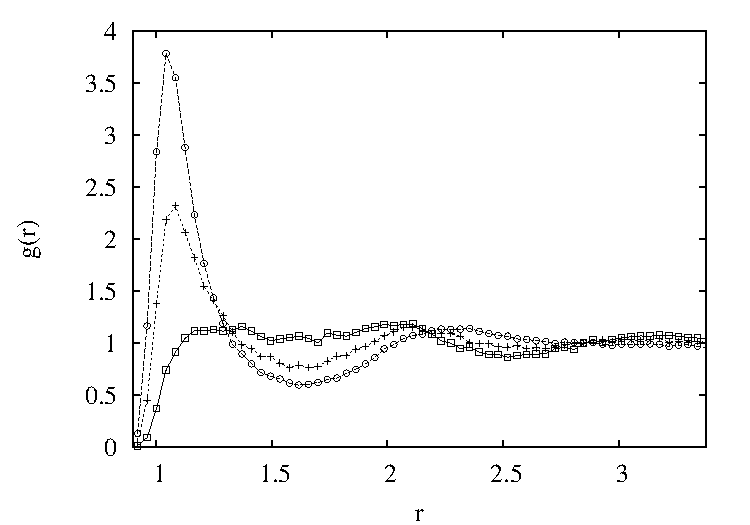
\includegraphics[width=0.7\textwidth]{figures/nacl-rdf.pdf}
  \caption{Radial distribution functions $g_{++}(r)$ between equal charges
    (rectangles) and $g_{+-}(r)$ for opposite charges (circles). The plus
    symbols denote $g(r)$ for an uncharged system.}
  \label{fig:rdf}
\end{figure}

The printing of the calculated radial distribution functions is simple. Add to the end of the
previous snippet the following lines:
\begin{tclcode}
set plot [open "rdf.data" "w"]
puts $plot "\# r rdf(r)"
foreach r $rlist rdf $avg_rdf { puts $plot "$r $rdf" }
close $plot
\end{tclcode}
This instructs the Tcl interpreter to write the \verb|avg_rdf| to the file \verb|rdf.data| in
gnuplot--compatible format. Fig.~\ref{fig:rdf} shows the resulting radial distribution functions,
averaged over 100 configurations. In addition, the distribution for a neutral
system is given, which can be obtained from our simulation script by simply
removing the command \verb|inter coulomb ...| and therefore not turning on P$^3$M.

The code example given before is still quite simple, and the reader is
encouraged to try to extend the example a little bit, e.~g. by using differently
sized particle, or changing the interactions. If something does not work, \es\
will give comprehensive error messages, which should make it easy to identify
mistakes. For real simulations, the simulation scripts can extend over thousands
of lines of code and contain automated adaption of parameters or online
analysis, up to automatic generation of data plots.  Parameters can be changed
arbitrarily during the simulation process, as needed for e.~g.\ simulated
annealing. The possibility to perform non--standard simulations without the need
of modifications to the simulation core was one of the main reasons why we
decided to use a script language for controlling the simulation core.

\section{\texttt{tutorial.tcl}}

In the directory \texttt{samples/} of the es{} sources, you will find
a well documented simulation script \texttt{tutorial.tcl}, which takes
you step by step through a slightly more complicated simulation of a
polyelectrolyte system. The basic structure of the script is however
the same as in the previous example and probably the same as the
structure of most \es{} simulation scripts.

Initially, some parameters and global variables are set, the
interactions are initialized, and particles are added. For this, the
script makes use of the \verb|polymer| command, which provides a
faster way to set up chain molecules.

The actual simulation falls apart again into two loops, the warmup
loop with increasing force capping, and the final simulation loop.
Note that the electrostatic interaction is only activated after
equilibrating the excluded volume interactions, which speeds up the
warmup phase. However, depending on the problem, this splitted warmup
may not be possible due to physical restrictions. \es{} cannot detect
these mistakes and it is your responsibility to find simulation
procedure suitable to your specific problem.

%%% Local Variables: 
%%% mode: latex
%%% TeX-master: "ug"
%%% End: 

% Copyright (C) 2010,2011,2012,2013 The ESPResSo project
% Copyright (C) 2002,2003,2004,2005,2006,2007,2008,2009,2010 
%   Max-Planck-Institute for Polymer Research, Theory Group
%  
% This file is part of ESPResSo.
%   
% ESPResSo is free software: you can redistribute it and/or modify it
% under the terms of the GNU General Public License as published by the
% Free Software Foundation, either version 3 of the License, or (at your
% option) any later version.
%  
% ESPResSo is distributed in the hope that it will be useful, but
% WITHOUT ANY WARRANTY; without even the implied warranty of
% MERCHANTABILITY or FITNESS FOR A PARTICULAR PURPOSE.  See the GNU
% General Public License for more details.
%  
% You should have received a copy of the GNU General Public License
% along with this program.  If not, see <http://www.gnu.org/licenses/>.
%
\chapter{Getting, compiling and running \es}
\label{chap:install}
\index{Installation|textbf}

This chapter will describe how to get, compile and run the \es
software.  

\es releases are available as source code packages from the \es home
page\footnote{\url{http://espressomd.org}}.  This is where new users
should get the code.  The code within release packages is tested and
known to run on a number of platforms.  Alternatively, people that
want to use the newest features of \es or that want to start
contributing to the software can instead obtain the current
development code via the version control system software
\textsf{git}\footnote{\url{http://git.org}} from \es's project page at
the Savannah GNU server
\footnote{\url{https://savannah.nongnu.org/projects/espressomd/}}.
This code might be not as well tested and documented as the release
code; it is recommended to use this code only if you have already
gained some experience in using \es.

Unlike most other software, no binary distributions of \es are
available, and the software is usually not installed globally for all
users.  Instead, users of \es should compile the software themselves.
\index{features} The reason for this is that it is possible to
activate and deactivate various features before compiling the code.
Some of these features are not compatible with each other, and some of
the features have a profound impact on the performance of the code.
Therefore it is not possible to build a single binary that can satisfy
all needs.  A user should always activate only those features that are
actually needed.  This means, however, that learning how to compile
\es is a necessary evil.  The build system of \es uses the GNU
autotools, which are developed since more than 20 years and allow to
compile software easily on a wide range of platforms.

\section{Running \texttt{configure}}
\label{sec:configure}
\index{configure}

\todo[inline]{Description of basic options: \keyword{CPPFLAGS},
  \keyword{CFLAGS}, \keyword{LDFLAGS}}

The first step of building \es is to run the shell script
\codebox{configure} which is to be found in the top level source
directory.  The script collects all the information required by the
compilation process.  It will determine how to use and where to find
the compiler, as well as the different libraries and tools required by
the compilation process, and it will test what compiler flags are to
be used.  The script will find out about most of these things
automatically.  If something is missing, it will complain and give
hints how to solve the problem.  The generic syntax of calling the
\codebox{configure} script is:
\begin{code}
configure [\var{options} ...] [\var{variable}=\var{value} ...]
\end{code}

If you are using the development source code from the \textsf{git}
repository, before you can call \codebox{configure}, it is necessary
to have the GNU autotools (\textsf{autoconf} and \textsf{automake})
installed. Then you can call the script \codebox{bootstrap.sh} from
the top level source directory, which will generate the
\codebox{configure} script.

\subsection{Source and build directories}
\label{ssec:builddir}
\index{build directory} \index{source directory}

Usually, when a program is compiled, the resulting binary files are
put into the same directory as the sources of the program.  In \es's
build system, the \emph{source directory} that contains all the source
files is completely separated from the \emph{build directory}, where
the files created by the build process are put.  The location of the
build directory is the current working directory at the time when
\codebox{configure} is called.  In this way, you can build several
variants of \es, each variant having different activated features, and
for as many platforms as you want.  All further commands concerning
compiling and running \es have to be called from the build directory.

\paragraph{Example}
When the source directory is \codebox{\$srcdir} (\ie the files where
unpacked to this directory), then the build directory can be set to
\codebox{\$builddir} by calling the \codebox{configure}-script from
there:
\begin{code}
cd $builddir
$srcdir/configure
make
Espresso
\end{code}

\subsection{Options}
\label{ssec:configureoptions}

\index{configure options} The behaviour of \codebox{configure} can be
controlled by the means of command line options.  In the following
only those command line options that are specific to \es will be
explained.  For a complete list of options and explanations thereof,
call
\begin{code}
configure --help
\end{code}

\begin{description}
\item[\texttt{--with-myconfig=MYCONFIG\_HEADER}] This option sets the
  name of the local configuration header (see \vref{sec:myconfig}). It
  defaults to ``\texttt{myconfig.h}''.
\item[\texttt{--with-mpi=\alt{\lit{yes} \asep \lit{no} \asep
      \lit{guess}}}/ \texttt{--without-mpi}] By default,
  \codebox{configure} will automatically determine whether an MPI
  compiler is available.  If it is, it will use it.  If you specify
  \codebox{--without-mpi} or \codebox{--with-mpi=no}, then MPI will
  not be used, even if it is available.
\item[\texttt{--with-efence} / \texttt{--without-efence}] Whether or
  not to use the ``electric fence'' memory debugging library.
  \footnote{\url{http://freshmeat.net/projects/efence/}} Efence is not
  used by default.
\item[\texttt{--with-tcl=TCL}] By default, \texttt{configure} will
  automatically determine which version of Tcl is used.  If the wrong
  version is chosen automatically, you can specify the name of the
  library with this option, \eg \texttt{tcl8.4}.
\item[\texttt{--with-tk=TK} / \texttt{--without-tk}] By default, the
  GUI toolkit Tk is not used by \es. This option can be used to
  activate Tk and to specify which Tk version to use, \eg{}
  \texttt{tk8.4}. If you only specify \texttt{--with-tk} and do not
  give a version number, \texttt{configure} will try to automatically
  deduce the right version.
\item[\texttt{--with-fftw} / \texttt{--without-fftw}] This can
  be used to specify whether the FFTW library is to be used, and which
  version.  By default, version 3 will be used if it is found,
  otherwise version 2 is used.  Note that quite a number of central
  features of \es require FFTW.
\item[\texttt{--with-cuda=path} / \texttt{--without-cuda}] This switch
  enables CUDA support. \texttt{path} should be the path to the CUDA
  directory, which can be omitted if it is the NVIDIA default path,
  \ie \texttt{/usr/local/cuda}. The variable \texttt{NVCCFLAGS} can
  be used to define compiler flags for the NVIDIA CUDA-compiler
  \texttt{nvcc}. For example, \texttt{NVCCFLAGS = "{}-gencode
    arch=compute_20,code=sm_20"{}} will compile code only for Fermi
  cards.  Default is to compile for compute models 1.1 and 2.0,
  i.e. everything with a G90 chip or newer.  Note that we require at
  least compute model 1.1.
\end{description}

\section{\texttt{make}: Compiling,  testing and installing \es}
\label{sec:make}

The command \texttt{make} is mainly used to compile the \es source
code, but it can do a number of other things. The generic syntax of
the \texttt{make} command is:
\begin{code}
make [\var{options}] [\var{target}...] [\var{variable}=\var{value}]
\end{code}
When no target is given, the target \texttt{all} is used. The
following targets are available:
\begin{description}
\item[\texttt{all}] Compiles the complete \es source code. The
  variable \lit{myconf} can be used to specify the name of the
  configuration header to be used.
\item[\texttt{check}] Runs the testsuite. By default, all available
  tests will be run on 1, 2, 3, 4, 6, or 8 processors. Which tests are
  run can be controlled by means of the variable \texttt{tests}, which
  processor numbers are to be used can be controlled via the variable
  \texttt{processors}. Note that depending on your MPI installation,
  MPI jobs can only be run in the queueing system, so that \es{} will
  not run from the command line. In that case, you may not be able to
  run the testsuite, or you have to directly submit the testsuite script
  \verb!testsuite/test.sh! to the queueing system.\\
  \textbf{Example:} \verb!make check tests="madelung.tcl" processors="1 2"!\\
  will run the test \texttt{madlung.tcl} on one and two processors.
\item[\texttt{clean}] Deletes all files that were created during the
  compilation.
\item[\texttt{mostlyclean}] Deletes most files that were created
  during the compilation. Will keep for example the built doxygen
  documentation and the \es{} binary.
\item[\texttt{dist}] Creates a \texttt{.tar.gz}-file of the \es{}
  sources.  This will include all source files as they currently are
  in the source directory, \ie{} it will include local changes.  This
  is useful to give your version of \es{} to other people.
  The variable \texttt{extra} can be used to specify additional
  files and directories that are to be included in the archive
  file. \\
  \textbf{Example:} \verb!make dist extra="myconfig.h internal"!\\
  will create the archive file and include the file
  \texttt{myconfig.h} and the directory \texttt{internal} with all
  files and subdirectories.
\item[\texttt{install}] Install \es. The variables \texttt{prefix} and
  \texttt{exec-prefix} can be used to specify the installation
  directories, otherwise the defaults defined by the
  \texttt{configure} script are used. \texttt{prefix} sets the prefix
  where all \es files are to be installed, \texttt{exec-prefix} sets
  the prefix where the executable files are to be installed and is
  required only when there is an architecture-specific directory.\\
  \textbf{Example:} \verb!make install prefix=/usr/local!\\
  will install all files below \texttt{/usr/local}.
\item[\texttt{uninstall}] Uninstalls \es, \ie removes all files that
  were installed during \texttt{make install}. The variables are
  identical to the variables of the \texttt{install}-target.
\item[\texttt{ug\ \ }] Creates the User guide in the \texttt{doc/ug}
  subdirectory (only when using the development sources).
\item[\texttt{dg\ \ }] Creates the Developers' guide in the
  \texttt{doc/dg} subdirectory (only when using the development
  sources).
\item[\texttt{doxygen\ \ }] Creates the Doxygen code documentation in the
  \texttt{doc/doxygen} subdirectory.
\item[\texttt{tutorials\ \ }] Creates the \es tutorials in the
  \texttt{doc/tutorials} subdirectory.
\item[\texttt{doc\ }] Creates all documentation in the \texttt{doc}
  subdirectory (only when using the development sources).
\end{description}

A number of options are available when calling \texttt{make}.  The
most interesting option is probably \texttt{-j \textit{num\_jobs}},
which can be used for parallel compilation on computers that have more
than one CPU or core.  \textit{num\_jobs} specifies the maximal number
of jobs that will be run.  Setting \textit{num\_jobs} to the number of
available processors speeds up the compilation process significantly.

\section{Running \es}
\label{sec:run}

When \es is found in your path, it can be run via
\begin{code}
Espresso [\var{tcl\_script} [\var{args}]]
\end{code}

\index{interactive mode} When \es{} is called without any arguments,
it is started in the interactive mode, where new commands can be
entered on the command line. When the name of a \textit{tcl\_script}
is given, the script is executed. \textit{N\_processors} is the number
of processors that are to be used. Any further arguments are passed to
the script. Note that depending on your MPI installation, MPI jobs can
only be run in the queueing system, so that \es will not run from
the command line.


\section{\texttt{myconfig.h}: Activating and deactivating features}
\label{sec:myconfig}

\index{features} \index{myconfig.h} \index{configuration header} \es
has a large number of features that can be compiled into the binary.
However, it is not recommended to actually compile in all possible
features, as this will slow down \es significantly.  Instead, compile
in only the features that are actually required.  A strong gain in
speed can be achieved, by disabling all non-bonded interactions except
for a single one, e.g. \feature{LENNARD_JONES}.  For the developers,
it is also possible to turn on or off a number of debugging messages.
The features and debug messages can be controlled via a configuration
header file that contains C-preprocessor declarations. Appendix
\vref{chap:features} lists and describes all available features.  When
no configuration header is provided by the user, a default header,
found in src/myconfig-default.h, will be used that turns on the
default features.  The file \texttt{myconfig-sample.h} in the source
directory contains a list of all possible features that can be copied
into your own configuration file.

When you distinguish between the build and the source directory, the
configuration header can be put in either of these. Note, however,
that when a configuration header is found in both directories, the one
in the build directory will be used.

By default, the configuration header is called \texttt{myconfig.h}.
The name of the configuration header can be changed either when the
\texttt{configure}-script is called with the option
\mbox{\texttt{--with-myconfig}} (see section \vref{sec:configure}), or
when \texttt{make} is called with the setting
\mbox{\texttt{myconfig=}\textit{myconfig\_header}} (see section
\vref{sec:make}).

The configuration header can be used to compile different binary
versions of \es with a different set of features from the same source
directory.  Suppose that you have a source directory \texttt{\$srcdir}
and two build directories \texttt{\$builddir1} and
\texttt{\$builddir2} that contain different configuration headers:

\begin{itemize}
\item \texttt{\$builddir1/myconfig.h}:
\begin{code}
#define ELECTROSTATICS
#define LENNARD-JONES
\end{code}

\item \texttt{\$builddir2/myconfig.h}:
\begin{code}
#define LJCOS
\end{code}
\end{itemize}

\noindent Then you can simply compile two different versions of \es via
\begin{code}
cd $builddir1
$srcdir/configure
make

cd $builddir2
$srcdir/configure
make
\end{code}


%%% Local Variables: 
%%% mode: latex
%%% TeX-master: "ug"
%%% End: 


% Copyright (C) 2010,2011,2012,2013,2014,2015,2016 The ESPResSo project
% Copyright (C) 2002,2003,2004,2005,2006,2007,2008,2009,2010 
%   Max-Planck-Institute for Polymer Research, Theory Group
%  
% This file is part of ESPResSo.
%   
% ESPResSo is free software: you can redistribute it and/or modify it
% under the terms of the GNU General Public License as published by the
% Free Software Foundation, either version 3 of the License, or (at your
% option) any later version.
%  
% ESPResSo is distributed in the hope that it will be useful, but
% WITHOUT ANY WARRANTY; without even the implied warranty of
% MERCHANTABILITY or FITNESS FOR A PARTICULAR PURPOSE.  See the GNU
% General Public License for more details.
%  
% You should have received a copy of the GNU General Public License
% along with this program.  If not, see <http://www.gnu.org/licenses/>.
%
\chapter{Setting up particles}
\label{chap:part}

\section{\keyword{part}: Creating single particles}
\newescommand{part}

\subsection{Defining particle properties}
\label{ssec:particleproperties}

\begin{pysyntax}
  \property{
    espressomd.System()
  }{
    part[\arg{pid}]
  }{
    type=\arg{int},
    pos=\arg{array of 3 floats},
    v=\arg{array of 3 floats},
    f=\arg{array of 3 floats},
    bonds=\arg{bond},
    mass=\arg{float},
    omega_lab=\arg{array of 3 floats},
    rinertia=\arg{array of 3 floats},
    omega_body=\arg{array of 3 floats},
    torque_lab=\arg{array of 3 floats},
    quat=\arg{array of 4 floats},
    %director=\arg{},
    q=\arg{float},
    virtual=\arg{int $\geq$ 0},
    vs_relative=\arg{tuple of int and float},
    vs_auto_relate_to=\arg{int},
    dip=\arg{array of 3 floats},
    dipm=\arg{float},
    fix=\arg{array of 3 ints},
    ext_force=\arg{array of 3 floats},
    ext_torque=\arg{array of 3 floats},
    exclude=\arg{list of ints},
    temp=\arg{float},
    gamma=\arg{float},
    gamma_rot=\arg{float},
    rotation=\arg{bool},
    swimming=\arg{dictionary \ttfamily \{
      `f_swim':\arg{float},
      `v_swim':\arg{float},
      `mode':\arg{``pusher''|``puller''},
      `dipole_length':\arg{float},
      `rotational_friction':\arg{float}\}}
  }
\end{pysyntax}
\begin{essyntax}
  part
  \var{pid}
  \opt{pos \var{x} \var{y} \var{z}}
  \opt{type \var{typeid}}
  \opt{v \var{vx} \var{vy} \var{vz}}
  \opt{f \var{fx} \var{fy} \var{fz}}
  \opt{bond \var{bondid} \var{pid2} \dots}
  \require{1}{\opt{q \var{charge}}}
  \require{2}{\opt{quat \var{q1} \var{q2} \var{q3} \var{q4}}}
  \require{2}{\opt{omega_body/lab \var{x} \var{y} \var{z}}}
  \require{2}{\opt{torque_body/lab \var{x} \var{y} \var{z}}}
  \require{2}{\opt{rinertia \var{x} \var{y} \var{z}}}
  \require{3}{\opt{\opt{un}fix \var{x} \var{y} \var{z}}}
  \require{3}{\opt{ext_force \var{x} \var{y} \var{z}}}
  \require{2,3}{\opt{ext_torque \var{x} \var{y} \var{z}}}
  \require{4}{\opt{exclude \var{pid2}\dots}}
  \require{4}{\opt{exclude delete \var{pid2}\dots}}
  \require{5}{\opt{mass \var{mass}}}
  \require{6}{\opt{dipm \var{moment}}}
  \require{6}{\opt{dip \var{dx} \var{dy} \var{dz}}}
  \require{7,8}{\opt{virtual \var{v}}}
  \require{8}{\opt{vs\_relative \var{pid} \par{distance}}}
  \require{8}{\opt{vs\_auto\_relate\_to \var{pid}}}
  \require{9}{\opt{temp \var{T}}}
  \require{9}{\opt{gamma \var{g}}}
  \require{2,9}{\opt{gamma\_rot \var{grot}}}
  \require{10}{\opt{rotation \var{rot}}}
  \require{11}{\opt{solvation \var{lA} \var{kA} \var{lB} \var{kB}}}
  \require{12}{\opt{swimming \alt{\alt{v_swim \var{v\_swim} \asep
          f_swim \var{f\_swim}} \asep off}}}
  \requirelong{12,13}{%
    \optlong{swimming
      \alt{%
        \alt{v_swim \var{v\_swim} \asep f_swim \var{f\_swim}}
        \alt{pusher \asep puller}
        dipole_length \var{dipole\_length}
        rotational_friction \var{rotational\_friction}
      \asep off}%
    }%
  }
  \begin{features}
    \required[1]{ELECTROSTATICS} 
    \required[2]{ROTATION}
    \required[3]{EXTERNAL_FORCES}
    \required[4]{EXCLUSION}
    \required[5]{MASS}
    \required[6]{DIPOLES}
    \required[7]{VIRTUAL\_SITES\_COM}
    \required[8]{VIRTUAL\_SITES\_RELATIVE}
    \required[9]{LANGEVIN\_PER\_PARTICLE}
    \required[10]{ROTATION\_PER\_PARTICLE}
    \required[11]{SHANCHEN}
    \required[12]{ENGINE}
    \required[13]{LB \MakeLowercase{\textrm{or}} LB_GPU}
  \end{features}
\end{essyntax}

This command modifies particle data, namely position, type (monomer,
ion, \dots), charge, velocity, force and bonds. Multiple properties can
be changed at once. If you add a new particle the position has to be
set first because of the spatial decomposition.

\begin{arguments}
\item[\var{pid}]
\item[\opt{pos \var{x} \var{y} \var{z}}] Sets the position of this
  particle to $(x,y,z)$.
\item[\opt{type \var{typeid}}] Restrictions:
  $\var{typeid} \geq 0$.\\ The
  \var{typeid} is used in the \keyword{inter} command
  (see section \vref{tcl:inter}) to define the parameters of the non
  bonded interactions between different kinds of particles.
\item[\opt{v \var{vx} \var{vy} \var{vz}}] Sets the velocity of
  this particle to $(vx,vy,vz)$. The velocity remains variable and will be changed
  during integration.
\item[\opt{f \var{fx} \var{fy} \var{fz}}] Set the force acting on this particle
  to $(fx,fy,fz)$. The force remains variable and will be changed during integration. 
  However, whereas the velocity is modified with respect to the velocity you set
  upon integration, the force it recomputed during the integration step and any 
  force set in this way is lost during the integration step.
\item[\opt{bond \var{bondid} \var{pid2}\dots}]
  Restrictions: \var{bondid} $\geq 0$; \var{pid2} must
  be an existing particle.  The \var{bondid} is used for
  the inter command to define bonded interactions.
\item[bond delete] Will delete all bonds attached to this particle.
\item[\opt{q \var{charge}}] Sets the charge of this particle to $q$.
\item[\opt{quat \var{q1} \var{q2} \var{q3} \var{q4}}] Sets the
  quaternion representation of the rotational position of this
  particle.
\item[\opt{omega_body} \var{x} \var{y} \var{z} \alt \opt{omega_body}
  \var{x} \var{y} \var{z}] The command \opt{omega_body} sets the
  angular momentum of this particle in the particle's co-rotating
  frame (or body frame) and the command \opt{omega_lab} sets it for
  the particle in the fixed frame (or laboratory frame). If you set
  the angular momentum of the particle in the lab frame, the
  orientation of the particle (\opt{quat}) must be set before invoking
  \opt{omega_lab}, otherwise the conversion from lab to body frame
  will not be handled properly.
\item[\opt{torque_body/lab \var{x} \var{y} \var{z}}] The command
  \opt{torque_body} sets the torque of this particle in the particle's
  co-rotating frame (or body frame) and the command \opt{torque_lab}
  sets it for the particle in the fixed frame (or laboratory
  frame). If you set the torque of the particle in the lab frame, the
  orientation of the particle (\opt{quat}) must be set before invoking
  \opt{torque_lab}, otherwise the conversion from lab to body frame
  will not be handled properly.
\item[\opt{rinertia \var{x} \var{y} \var{z}}] Sets the diagonal
  elements of this particles rotational inertia tensor. These
  correspond with the inertial moments along the coordinate axes in
  the particle's co-rotating coordinate system. When the particle's
  quaternions are set to 1 0 0 0, the co-rotating and the fixed (lab)
  frame are co-aligned.
\item[\opt{fix \var{x} \var{y} \var{z}}] Fixes the particle in space.
  By supplying a set of 3 integers as arguments it is possible to fix
  motion in \var{x}, \var{y}, or \var{z} coordinates independently. For
  example \var{fix} 0 0 1 will fix motion only in z. Note that
  \var{fix} without arguments is equivalent to \var{fix} 1 1 1.
\item[\opt{unfix}] Release any external influence from the particle.
\item[\opt{ext_force \var{x} \var{y} \var{z}}]
  An additional external force is applied to the particle.
\item[\opt{ext_torque \var{x} \var{y} \var{z}}]
  An additional external torque is applied to the particle. This torque is specified
  in the laboratory frame!
\item[\opt{exclude \var{pid2}\dots+}] Restrictions:
  \var{pid2} must be an existing particle.  Between the
  current particle an the exclusion partner(s), no nonbonded
  interactions are calculated. Note that unlike bonds, exclusions are
  stored with both partners. Therefore this command adds the defined
  exclusions to both partners.
\item[\opt{exclude delete \var{pid2}\dots}] Searches for the
  given exclusion and deletes it. Again deletes the exclusion with
  both partners.
\item[\opt{mass \var{mass}}] Sets the mass of this particle to $mass$. If not
  set, all particles have a mass of 1 in reduced units.
\item[\opt{dipm \var{moment}}] Sets the dipol moment of this particle to $moment$.
\item[\opt{dip \var{dx} \var{dy} \var{dz}}] Sets the orientation of the
  dipole axis to $(dx,dy,dz)$.
\item[\opt{virtual \var{v}}] Declares the particles as virtual (1) or
  non-virtual (0, default). Please read chapter \ref{sec:virtual}
  before using virtual sites.
\item[\opt{vs\_auto\_relate\_to \var{pid}}] Automatically relates a
  virtual site to a non-virtual particle for the ``relative''
  implementation of virtual sites. \var{pid} is the id of the particle
  to which the virtual site should be related.
\item[\opt{vs\_relative \var{pid} \var{distance}}] Allows for manual
  access to the attributes of virtual sites in the ``relative''
  implementation. \var{pid} denotes the id of the particle to which
  this virtual site is related and \var{distance} the distance between
  non-virtual and virtual particle.
\item[\opt{temp \var{T}}] If used in combination with the Langevin
  thermostat (as documented in section \ref{sec:thermostat}), sets the
  temperature \var{T} individually for the particle with id
  \var{pid}. This allows to simulate systems containing particles of
  different temperatures. Caution: this has no influence on any other
  thermostat then the Langevin thermostat.
\item[\opt{gamma \var{g}}] If used in combination with the Langevin
  thermostat (as documented in section \ref{sec:thermostat}), sets the
  frictional coefficient \var{T} individually for the particle with id
  \var{pid}. This allows to simulate systems containing particles with
  different diffusion constants. Caution: this has no influence on any
  other thermostat then the Langevin thermostat.
\item[\opt{rotation \var{rot}}] Specifies whether a particle's
  rotational degrees of freedom along the different axes in the particle's body-fixed frame are integrated or not.
  If set to zero, rotation is disabled entirely, and the content of the torque and omega variables
  are meaningless. 
  Rotation of a particular axis is turned on by adding up the corresponding flags: x=2, y=4, z=8.
  To enable rotation around all axis, use a value of 2+4+8=14. This is also the default.
\item[\opt{solvation \var{lA} \var{kA} \var{lB} \var{kB}}] Sets the
  four solvation coupling constants for the two components of a
  Shan-Chen fluid, as documented in Section \ref{sec:scmd-coupling}.
\item[\opt{swimming \alt{\alt{v_swim \var{v\_swim} \asep f_swim
        \var{f\_swim}} \asep off}}] Enables the particle to be
  self-propelled in the direction determined by its quaternion. For
  setting the quaternion of the particle see \keyword{quat}. The
  self-propulsion speed will relax to a constant velocity, that is
  specified by \keyword{v_swim}. Alternatively it is possible to
  achieve a constant velocity by imposing a constant force term
  \keyword{f_swim} that is balanced by friction of a (Langevin)
  thermostat. The way the velocity of the particle decays to the
  constant terminal velocity in either of these methods is completely
  determined by the friction coefficient. You may only set one of the
  possibilities \keyword{v_swim} \emph{or} \keyword{f_swim} as you
  cannot relax to constant force \emph{and} constant velocity at the
  same time. The option \keyword{off} (re)sets \var{v\_swim} and
  \var{f\_swim} both to $0.0$ and thus disables swimming. This option
  applies to all non-lattice-Boltzmann thermostats. Note that there is
  no real difference between \keyword{v_swim} and \keyword{f_swim},
  since the latter may aways be chosen such that the same terminal
  velocity is achieved for a given friction coefficient.
\item[{\parbox[t]{\linewidth}{\optlong{swimming \alt{%
          \alt{v_swim \var{v\_swim} \asep f_swim \var{f\_swim}}
          \alt{pusher \asep puller} dipole_length \var{dipole\_length}
          rotational_friction \var{rotational\_friction} \asep off}%
      }}}] For an explanation of the parameters \keyword{v_swim},
  \keyword{f_swim} and \keyword{off} see the previous item. In
  lattice-Boltzmann self-propulsion is less trivial than for normal
  MD, because the self-propulsion is achieved by a force-free
  mechanism, which has strong implications for the far-field
  hydrodynamic flow field induced by the self-propelled particle. In
  \es{} only the dipolar component of the flow field of an active
  particle is taken into account. This flow field can be generated by
  a \emph{pushing} or a \emph{pulling} mechanism, leading to change in
  the sign of the dipolar flow field with respect to the direction of
  motion. You can specify the nature of the particle's flow field by
  using the keywords \keyword{pusher} or \keyword{puller}. You will
  also need to specify a \var{dipole\_length} which determines the
  distance of the source of propulsion from the particle's
  center. Note that you should not put this distance to zero; \es{}
  (currently) does not support mathematical dipole flow fields. The
  key \keyword{rotational_friction} can be used to set the friction
  that causes the orientation of the particle to change in shear
  flow. The torque on the particle is determined by taking the cross
  product of the difference between the fluid velocity at the center
  of the particle and at the source point and the vector connecting
  the center and source.

  \noindent
  You may ask: ``Why are there two methods \var{v\_swim} and
  \var{f\_swim} for the self-propulsion using the lattice-Bolzmann
  algorithm?'' The answer is straightforward. When a particle is
  accelerating, it has a monopolar flow-field contribution which
  vanishes when it reaches its terminal velocity (for which there will
  only be a dipolar flow field). The major difference between the
  above two methods is that with \var{v\_swim} the flow field
  \emph{only} has a monopolar moment and \emph{only} while the
  particle is accelerating. As soon as the particle reaches a constant
  speed (given by \var{v\_swim}) this monopolar moment is gone and the
  flow field is zero! In contrast, \var{f\_swim} always, i.e., while
  accelerating \emph{and} while swimming at constant force possesses a
  dipolar flow field.

  \noindent
  \fbox{\parbox{\linewidth-2\fboxsep-2\fboxrule}{%
      Please note that even though swimming is interoperable with the
      CPU version of LB it is only supported on \emph{one} Open MPI
      node, i.e.\ $\text{\keyword{n_nodes}} = 1$.%
    }}
\end{arguments}

\warning{The options \opt{omega}, \opt{torque}, and \opt{tbf} are
  deprecated and will be removed in some future version.}

\subsection{Getting particle properties}
\index{Lees-Edwards Boundaries}
\begin{essyntax}
  \variant{1}
  part \var{pid} print
  \optlong{\alt{id \asep pos \asep type \asep folded_position \asep 
      type \asep q \asep v \asep f \asep torque_body \asep torque_lab 
      \asep body_frame_velocity \asep fix \asep ext_force 
      \asep ext_torque \asep bond \asep exclusions 
      \mbox{connections \opt{\var{range}}} \asep swimming}}\dots
  \variant{2} part
\end{essyntax}

Variant \variant{1} will return a list of the specified properties of
particle \var{pid}, or all properties, if no keyword is
specified.  Variant \variant{2} will return a list of all properties
of all particles.

Note that there is a difference between the \keyword{*_body} and
\keyword{*_lab}.  The first prints the variable in the co-rotating
frame, whereas the second gives the variable in the stationary frame,
the body and laboratory frames, respectively. One would typically want
to output the variable in the laboratory frame, since it is the frame
of interest. However for some tests involving reading and writing the
variable it may be desireable to know it in the body frame as well. Be
careful with reading and writing, if you write in the lab frame, then
read in the lab frame. If you are setting the variable in the lab
frame, the orientation of the particle's \keyword{quat} must be set
before, otherwise the conversion from lab to body frame will not be
handled properly.  Also be careful about the order in which you write
and read in data from a blockfile, for instance if you output the
variable in both frames!

The \keyword{body_frame_velocity} command is a print-only command that
gives the velocity in the body frame, which can be useful for 
determining the translational diffusion tensor of an anisotropic 
particle via the velocity auto-correlation (Green-Kubo) method.

\minisec{Example}
\begin{code}
part 40 print id pos q bonds
\end{code}
will return a list like
\begin{tclcode}
40 8.849 1.8172 1.4677 1.0 {}
\end{tclcode}
This routine is primarily intended for effective use in Tcl scripts.

When the keyword \keyword{connection} is specified, it returns the
connectivity of the particle up to \var{range} (defaults to 1). For
particle 5 in a linear chain the result up to \var{range} = 3 would
look like:
\begin{tclcode}
{ { 4 } { 6 } } { { 4 3 } { 6 7 } } { {4 3 2 } { 6 7 8 } } 
\end{tclcode}
The function is useful when you want to create bonded interactions to
all other particles a certain particle is connected to. Note that this
output can not be used as input to the part command. Check results if
you use them in ring structures.

If none of the options is specified, it returns all properties of the
particle, if it exists, in the form
\begin{tclcode}
  0 pos 2.1 6.4 3.1 type 0 q -1.0 v 0.0 0.0 0.0 f 0.0 0.0 0.0
  bonds { {0 480} {0 368} ... } 
\end{tclcode}
which may be used as an input to this function later on. The first
integer is the particle number.

Variant \variant{2} returns the properties of all stored particles in
a tcl-list with the same format as specified above:
\begin{tclcode}
{0 pos 2.1 6.4 3.1 type 0 q -1.0 v 0.0 0.0 0.0 f 0.0 0.0 0.0
 bonds{{0 480}{0 368}...}} 
{1 pos 1.0 2.0 3.0 type 0 q 1.0 v 0.0 0.0 0.0 f 0.0 0.0 0.0
 bonds{{0 340}{0 83}...}} 
{2...{{...}...}}
{3...{{...}...}}
...
\end{tclcode}

When using \texttt{pos}, the particle position returned is {\bf
  unfolded}, for convenience in diffusion calculations etc.  Note that
therefore blockfiles will contain imaged positions, but un-imaged
velocities, which should not be interpreted together. However, that is
fine for restoring the simulation, since the particled data is loaded
the same way.

\subsection{Deleting  particles}
\label{tcl:part:delete}

\todo{What is the syntax of variant 3?}
\begin{essyntax}
  \variant{1} part \var{pid} delete
  \variant{2} part deleteall
\end{essyntax}

In variant \variant{1}, the particle \var{pid} is deleted
and all bonds referencing it.  Variant \variant{2} will delete all
particles currently present in the simulation. Variant \variant{3}
will delete all currently defined exclusions.

\subsection{Exclusions}

\begin{essyntax}
  \variant{1} part auto\_exclusions \opt{\var{range}}
  \variant{2} part delete\_exclusions
  \begin{features}
    \required{EXCLUSIONS} 
  \end{features}
\end{essyntax}


Variant \variant{1} will create exclusions for all particles pairs
connected by not more than \var{range} bonds (\var{range} defaults to
2). This is typically used in atomistic simulations, where nearest and
next nearest neighbour interactions along the chain have to be omitted
since they are included in the bonding potentials. For example, if the
system contains particles $0$ \dots $100$, where particle $n$ is
bonded to particle $n-1$ for $1 \leq n \leq 100$, then it will result
in the exclusions:
\begin{itemize}
  \item particle 1 does not interact with particles 2 and 3
  \item particle 2 does not interact with particles 1, 3 and 4
  \item particle 3 does not interact with particles 1, 2, 4 and 5
  \item ...
\end{itemize}

Variant \variant{2} deletes all exclusions currently present in the
system.

\section{Creating groups of particle}

\subsection{\texttt{polymer}: Setting up polymer chains}

\newescommand{polymer}
\begin{essyntax}
  polymer 
  \var{num\_polymers} \var{monomers\_per\_chain}
  \var{bond\_length}\\
  \opt{start \var{pid}} 
  \opt{pos \var{x} \var{y} \var{z}}
  \opt{mode \alt{RW \asep SAW \asep PSAW} 
    \opt{\var{shield} \opt{\var{try_\mathrm{max}}}}} 
  \require{1}{\opt{charge \var{q}}} 
  \require{1}{\opt{distance \var{d_\mathrm{charged}}}}
  \opt{types \var{typeid_\mathrm{neutral}}
    \opt{\var{typeid_\mathrm{charged}}}} 
  \opt{bond \var{bondid}} 
  \opt{angle \var{\phi} \opt{\var{\theta} \opt{\var{x} \var{y}
        \var{z}}}}
  \require{2}{\opt{constraints}}
  \begin{features}
    \required[1]{ELECTROSTATICS}
    \required[2]{CONSTRAINTS}
  \end{features}
\end{essyntax}

This command will create \var{num\_polymers} polymer or
polyelectrolyte chains with \var{monomers\_per\_chain} monomers per
chain. The length of the bond between two adjacent monomers will be
set up to be \var{bond\_length}.

\begin{arguments}
\item[\var{num\_polymers}] Sets the number of polymer chains.
\item[\var{monomers\_per\_chain}] Sets the number of monomers per
  chain.
\item[\var{bond\_length}] Sets the initial distance between two
  adjacent monomers. The distance during the course of the simulation
  depends on the applied potentials. For fixed bond length please
  refer to the Rattle Shake algorithm\cite{andersen83a}.  The algorithm
  is based on Verlet algorithm and satisfy internal constraints for
  molecular models with internal constrains, using Lagrange
  multipliers.
\item[\opt{start \var{pid}}] Sets the particle number of the
  start monomer to be used with the \keyword{part} command. This
  defaults to 0.

\item[\opt{pos \var{x} \var{y} \var{z}}] Sets the position of the
  first monomer in the chain to \var{x}, \var{y}, \var{z} (defaults to
  a randomly chosen value)
  
\item[\opt{mode \alt{RW  \asep  PSAW  \asep  SAW} \opt{\var{shield}
      \opt{\var{try_\mathrm{max}}}}}]
  Selects the setup mode:
  \begin{description}
  \item[\keyword{RW} (Random walk)] The monomers are
    randomly placed by a random walk with a steps size of
    \var{bond_length}.
  \item[\keyword{PSAW} (Pruned self-avoiding walk)] The position of a
    monomer is randomly chosen in a distance of \var{bond\_length} to
    the previous monomer. If the position is closer to another
    particle than \var{shield}, the attempt is repeated up to
    \var{try_\mathrm{max}} times. Note, that this is not a real
    self-avoiding random walk, as the particle distribution is not the
    same. If you want a real self-avoiding walk, use the \keyword{SAW}
    mode.  However, \keyword{PSAW} is several orders of magnitude
    faster than \keyword{SAW}, especially for long chains.
  \item[\keyword{SAW} (Self-avoiding random walk)] The positions of
    the monomers are chosen as in the plain random walk. However, if
    this results in a chain that has a monomer that is closer to
    another particle than \var{shield}, a new attempt of setting up
    the whole chain is done, up to \var{try_\mathrm{max}} times.
  \end{description}
  The default for the mode is \keyword{RW}, the default for the
  \var{shield} is $1.0$, and the default for \var{try_\mathrm{max}} is
  $30000$, which is usually enough for \keyword{PSAW}. Depending on
  the length of the chain, for the \keyword{SAW} mode,
  \var{try_\mathrm{max}} has to be increased by several orders of
  magnitude.
\item[\opt{charge \var{valency}}] Sets the valency of the charged
  monomers.  If the valency of the charged polymers \var{valency} is
  smaller than $10^{-10}$, the charge is assumed to be zero, and the
  types are set to $\var{typeid_\mathrm{charged}} =
  \var{typeid_\mathrm{neutral}}$. If charge is not set, it defaults to
  0.0.
\item[\opt{distance \var{d_\mathrm{charged}}}] Sets the stride
  between the indices of two charged monomers. This defaults defaults
  to 1, meaning that all monomers in the chain are charged.
\item[\opt{types \var{typeid_\mathrm{neutral}}
    \var{typeid_\mathrm{charged}}}] Sets the type ids of the neutral
    and charged monomer types to be used with the \keyword{part}
    command. If only \var{typeid_\mathrm{neutral}} is defined,
    \var{typeid_\mathrm{charged}} defaults to $1$. If the option is
    omitted, both monomer types default to $0$.
  \item[\opt{bond \var{bondid}}] Sets the type number of the bonded
    interaction to be set up between the monomers. This defaults to
    $0$.  Any bonded interaction, no matter how many bonding-partners
    needed, is stored with the second particle in this bond. See
    chapter \ref{sec:inter-bonded}.
  \item[\opt{angle \var{\phi} [\var{\theta} [\var{x} \var{y}
      \var{z}]]}] Allows for setting up helices or planar polymers:
    \var{\phi} and \var{theta} are the angles between adjacent bonds.
    \var{x}, \var{y} and \var{z} set the position of the second
    monomer of the first chain.
  \item[\opt{constraints}] If this option is specified, the particle setup-up
  tries to obey previously defined constraints (see section \vref{sec:constraint}).
\end{arguments}

\subsection{\texttt{counterions}: Setting up counterions}
\newescommand{counterions}
\begin{essyntax}
  counterions
  \var{N} 
  \opt{start \var{pid}} 
  \opt{mode \alt{SAW \asep RW} \opt{\var{shield} \opt{\var{try_\mathrm{max}} }}} 
  \require{1}{\opt{charge \var{val}}}
  \opt{type \var{typeid}}
  \begin{features}
    \required[1]{ELECTROSTATICS}
  \end{features}
\end{essyntax}
This command will create \var{N} counterions in the simulation box.
\begin{arguments}
\item[\opt{start \var{pid}}] Sets the particle id of the first
  counterion.  It defaults to the current number of particles, \ie
  counterions are placed after all previously defined particles.
\item[\opt{mode \alt{SAW \asep RW} \opt{\var{shield}
      \opt{\var{try_\mathrm{max}} }}}] Specifies the setup method to
  place the counterions. It defaults to \keyword{SAW}. See the
  \keyword{polymer} command for a detailed description.
\item[\opt{charge \var{val}}] Specifies the charge of the counterions.
  If not set, it defaults to $-1.0$.
\item[\opt{type \var{typeid}}] Specifies the particle type of the
  counterions. It defaults to $2$.
\end{arguments}

\smallskip
\subsection{\texttt{salt}: Setting up salt ions}
\newescommand{salt}
\begin{essyntax}
  salt 
  \var{N_+} \var{N_-} 
  \opt{start \var{pid}} 
  \opt{mode \alt{SAW \asep RW} \opt{\var{shield} \opt{\var{try_\mathrm{max}}}}}
  \require{1}{\opt{charges \var{val_+} \opt{\var{val_-}}}} 
  \opt{types \var{typeid_+} \opt{\var{typeid_-}}}
  \opt{rad \var{r}}
  \begin{features}
    \required[1]{ELECTROSTATICS}
  \end{features}
\end{essyntax}

Create \var{N_+} positively and \var{N_-} negatively charged salt ions
of charge \var{val_+} and \var{val_-} within the simulation box.
\begin{arguments}
\item[\opt{start \var{pid}}] Sets the particle id of the first
  (positively charged) salt ion. It defaults to the current number of
  particles.
\item[\opt{mode \alt{SAW \asep RW} \opt{\var{shield}
      \opt{\var{try_\mathrm{max}} }}}] Specifies the setup method to
  place the counterions. It defaults to \keyword{SAW}. See the
  \keyword{polymer} command for a detailed description.
\item[\opt{charge \var{val_+} \opt{\var{val_-}}}] Sets the charge of
  the positive salt ions to \var{val_+} and the one of the negatively
  charged salt ions to \var{val_-}. If not set, the values default to
  $1.0$ and $-1.0$, respectively.
\item[\opt{type \var{typeid_+} \opt{\var{typeid_-}}}] Specifies the
  particle type of the salt ions. It defaults to $3$ respectively $4$.
\item[\opt{rad \var{r}}] The salt ions are only placed in a
  sphere with radius \var{r} around the origin.
\end{arguments}


\subsection{\texttt{diamond}: Setting up diamond polymer networks}
\newescommand{diamond}
\begin{essyntax}
  diamond 
  \var{a} \var{bond\_length} \var{monomers\_per\_chain} 
  \opt{counterions \var{N_\mathrm{CI}}}\\ 
  \require{1}{\opt{charges \var{val_\mathrm{node}}
      \var{val_\mathrm{monomer}} \var{val_\mathrm{CI}}}}
  \require{1}{\opt{distance \var{d_\mathrm{charged}}}}
  \opt{nonet}
  \begin{features}
    \required[1]{ELECTROSTATICS}
  \end{features}
\end{essyntax}

Creates a diamond-shaped polymer network with 8 tetra-functional nodes
connected by $2*8$ polymer chains of length \var{monomers\_per\_chain} in 
a unit cell of length \var{a}. Chain monomers are placed at a mutual distance \var{bond\_length}
along the vector connecting network nodes.
The polymer is created starting from particle ID 0. Nodes are assigned type 0,
monomers (both charged and uncharged) are type 1 and counterions type 2.
For inter-particle bonds interaction $0$ is taken which must be a two-particle bond.

\begin{figure}[ht]
  \label{fig:diamond}
  \begin{center}
  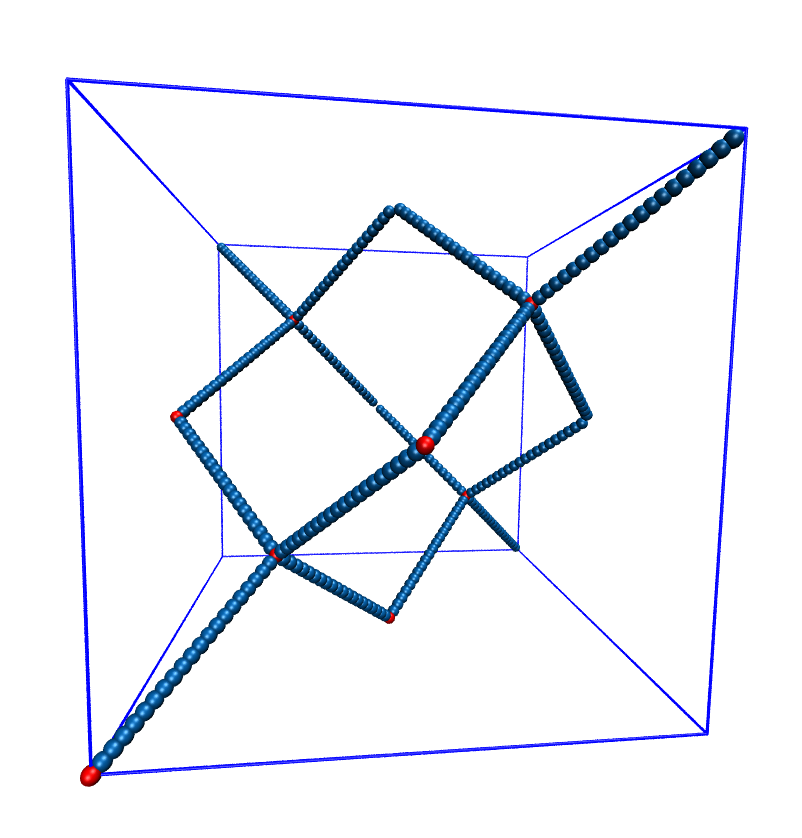
\includegraphics[height=6cm]{figures/diamond}
  \caption{Diamond-like polymer network with \var{monomers\_per\_chain}=15.}
  \end{center}
\end{figure}

\begin{arguments}
\item[\var{a}] Determines the size of the of the unit cell.
\item[\var{bond\_length}] Specifies the bond length of the polymer
  chains connecting the 8 tetra-functional nodes.
\item[\var{monomers\_per\_chain}] Sets the number of chain monomers
  between the functional nodes.
\item[\opt{counterions \var{N_\mathrm{CI}}}] Adds \var{N_\mathrm{CI}}
  counterions to the system.
\item[\opt{charges \var{val_\mathrm{node}} \var{val_\mathrm{monomer}}
    \var{val_\mathrm{CI}}}] Sets the charge of the nodes to
  \var{val_\mathrm{node}}, the charge of the connecting monomers to
  \var{val_\mathrm{monomer}}, and the charge of the counterions to
  \var{val_\mathrm{CI}}.
\item[\opt{distance \var{d_\mathrm{charged}}}] Specifies the distance
  between charged monomers along the interconnecting chains. If
  $\var{d_\mathrm{charged}} > 1$ the remaining chain monomers are
  uncharged.
  \item[\opt{nonet}] Do not create bonds between the chains.
\end{arguments}


\subsection{\texttt{icosaeder}: Setting up an icosaeder}
\newescommand{icosaeder}
\begin{essyntax}
  icosaeder 
  \var{a} \var{monomers\_per\_chain} 
  \opt{counterions \var{N_\mathrm{CI}}} 
  \require{1}{\opt{charges \var{val_\mathrm{monomers}} \var{val_\mathrm{CI}}}}
  \require{1}{\opt{distance \var{d_\mathrm{charged}}}}
  \begin{features}
    \required[1]{ELECTROSTATICS}
  \end{features}
\end{essyntax}

Creates a modified icosaeder to model a fullerene (or soccer ball).
The edges are modeled by polymer chains connected at the corners of
the icosaeder. For inter-particle bonds interaction $0$ is taken which
must be a two-particle bond. Two particle types are used for the
pentagons and the interconnecting links. For an example, see figure \ref{fig:fullerene}.

\begin{figure}[ht]
 \begin{center}
  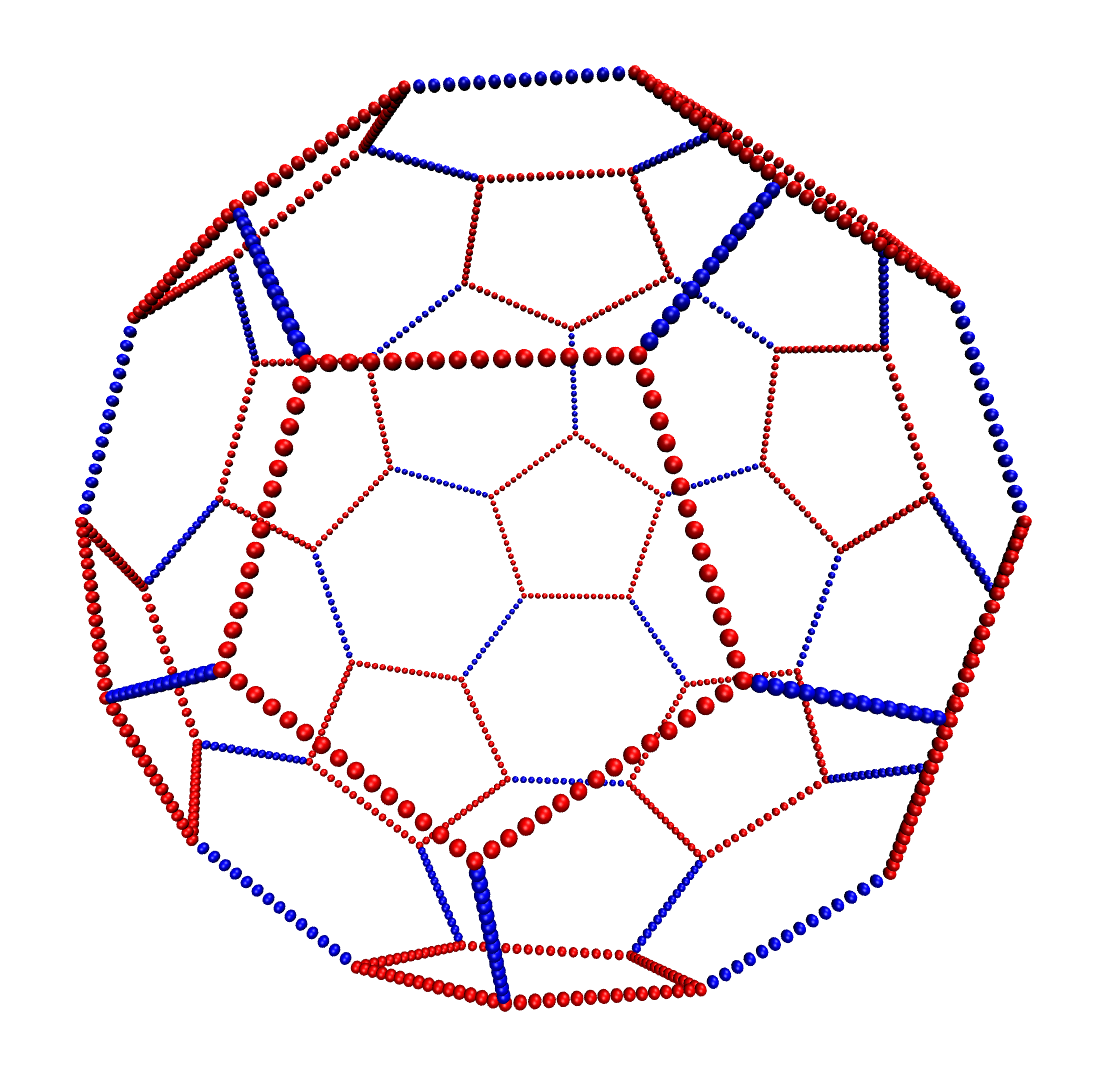
\includegraphics[height=6cm]{figures/fullerene}
  \caption{Icosaeder with \var{monomers\_per\_chain}=15.}
  \label{fig:fullerene}
  \end{center}
\end{figure}

\begin{arguments}
\item[\var{a}] Length of the links. Defines the size of the icosaeder.
\item[\var{monomers\_per\_chain}] Specifies the number of chain monomers along one edge.
\item[\opt{counterions \var{N_\mathrm{CI}}}] Specifies the number of
  counterions to be placed into the system.
\item[\opt{charges \var{val_\mathrm{monomers}} \var{val_\mathrm{CI}}}]
  Set the charges of the monomers to \var{val_\mathrm{monomers}} and
  the charges of the counterions to \var{val_\mathrm{CI}}.
\item[\opt{distance \var{d_\mathrm{charged}}}] Specifies the distance
  between two charged monomer along the edge. If
  $\var{d_\mathrm{charged}} > 1$ the remaining monomers are uncharged.
\end{arguments}

\subsection{\texttt{crosslink}: Cross-linking polymers}
\newescommand{crosslink}
\begin{essyntax}
  crosslink 
  \var{num\_polymer} \var{monomers\_per\_chain} 
  \opt{start \var{pid}} 
  \opt{catch \var{r_\mathrm{catch}}}
  \opt{distLink \var{link\_dist}} 
  \opt{distChain \var{chain\_dist}} 
  \opt{FENE \var{bondid}} 
  \opt{trials \var{try_\mathrm{max}}} 
\end{essyntax}

Attempts to end-crosslink the current configuration of
\var{num\_polymer} equally long polymers with
\var{monomers\_per\_chain} monomers each, returning how many ends are
successfully connected.

\begin{arguments}
\item[\opt{start \var{pid}}] \var{pid} specifies the first monomer of
  the chains to be linked. It has to be specified if the polymers do
  not start at id 0.
\item[\opt{catch \var{r_catch}}] Set the radius around each monomer
  which is searched for possible new monomers to connect to.
  \var{r_\mathrm{catch}} defaults to $1.9$.
\item[\opt{distLink \var{link\_dist}}] The minimal distance of two
  interconnecting links. It defaults to $2$.
\item[\opt{distChain \var{chain\_dist}}] The minimal distance for an
  interconnection along the same chain. It defaults to $0$. If set to
  \var{monomers\_per\_chain}, no interchain connections are created.
\item[\opt{FENE \var{bondid}}] Sets the bond type for the connections
  to \var{bondid}.
\item[\opt{trials \var{try_\mathrm{max}}}] If not specified,
  \var{try_\mathrm{max}} defaults to $30000$.
\end{arguments}

\subsection{\texttt{copy\_particles}: copying a set of particles}
\newescommand[copy-particles]{copy\_particles}
\begin{essyntax}
  copy_particles
  \opt{set \var{id1} \var{id2} \dots \asep range \var{from} {to} \dots} 
  \opt{shift \var{s\_x} \var{s\_y} \var{s\_z}}
\end{essyntax}

Copy a group of particles including their bonds. Positions can be
\opt{shift}ed by an offset $(\var{s\_x}, \var{s\_y}, \var{s\_z})$,
otherwise the copied set is at exactly the same position as the
original set. The particles can be given as a combination of
\opt{list}s or \opt{range}s. The new particles obtain in any case
consecutive identities after the largest current identity. The mapping
of the particles is returned as a list of old-new pairs, which can be
conveniently read into an array:
\begin{tclcode}
array set newidentities [copy_particles ...]
puts "particle 42 is now at position $newidentities(42)"
\end{tclcode} %$

Bonds within the defined particle set are copied with translated identities,
but not bonds with particles outside the list. That is, if the
particle set corresponds to a molecule, intramolecular bonds are
preserved, but not intermolecular ones.

Examples of use:\\
\begin{tclcode}
  copy_particles set {1 2 3 4} shift 0.0 0.0 0.0
  copy_particles set {1 2} set {3 4}
  copy_particles range 1 4
\end{tclcode}
All these examples do the same---making exact copies of particles 1 through 4.

\noindent
\fbox{\parbox{\linewidth-2\fboxsep-2\fboxrule}{%
    Please note that \keyword{copy_particles} only works if only
    fundamental particle properties are used, such as \keyword{pos},
    \keyword{type}, etc.\ as the \keyword{copy_particles} procedure
    only possesses parsers for these.  Other properties, such as
    \keyword{quatu} cannot be parsed and will thus lead to an error.%
  }}

\section{\texttt{constraint}: Setting up constraints}\label{sec:constraint}
\newescommand{constraint}

\begin{essyntax}
  \variant{1} 
  constraint wall normal \var{n_x} \var{n_y} \var{n_z} 
  dist \var{d} type \var{id} \opt{penetrable \var{flag}} \opt{reflecting
  \var{flag}} \opt{only_positive \var{flag}} \opt{tunable_slip \var{flag}}
  
  \variant{2}
  constraint sphere center \var{c_x} \var{c_y} \var{c_z} 
  radius \var{rad} direction \var{direction} type \var{id} \opt{penetrable \var{flag}} \opt{reflecting \var{flag}}
  
  \variant{3}
  constraint cylinder center \var{c_x} \var{c_y} \var{c_z} 
  axis \var{n_x} \var{n_y} \var{n_z} 
  radius \var{rad} length \var{length} 
  direction \var{direction} 
  type \var{id}  \opt{penetrable \var{flag}} \opt{reflecting \var{flag}}
  
  \variant{4}
  constraint rhomboid corner \var{p_x} \var{p_y} \var{p_z} 
  a \var{a_x} \var{a_y} \var{a_z} 
  b \var{b_x} \var{b_y} \var{b_z} \\
  c \var{c_x} \var{c_y} \var{c_z} 
  direction \var{direction} 
  type \var{id}  \opt{penetrable \var{flag}} \opt{reflecting \var{flag}}
  
  \variant{5}
  constraint maze nsphere \var{n} 
  dim \var{d} sphrad \var{r_s} cylrad \var{r_c}
  type \var{id} \opt{penetrable \var{flag}}
  
  \variant{6}  
  constraint pore center \var{c_x} \var{c_y} \var{c_z} 
  axis \var{n_x} \var{n_y} \var{n_z} 
  radius \var{rad} \opt{outer_radius \var{rad_S}} 
  \opt{smoothing_radius \var{rad_S}} length \var{length} 
  type \var{id} 

  \variant{7}
  constraint stomatocyte center \var{x} \var{y} \var{z} orientation \var{ox} \var{oy} \var{oz}
  outer_radius \var{Ro} inner_radius \var{Ri} layer_width \var{w} direction \var{direction} 
  type \var{id} \opt{penetrable \var{flag}} \opt{reflecting \var{flag}}
  
  \variant{8}
  constraint slitpore
  pore_mouth \var{z} \
             channel_width \var{c} \
             pore_width \var{w} \
             pore_length \var{l} \
             upper_smoothing_radius \var{us} \
             lower_smoothing_radius \var{ls} 
  
  
  \require{1}{%
    \variant{9}
    constraint rod center \var{c_x} \var{c_y} 
    lambda \var{lambda}
  } 
  
  \require{1}{%
    \variant{10}
    constraint plate height \var{h}
    sigma \var{sigma} 
  }
  
  \require{2,3}{%
    \variant{11}
    constraint ext_magn_field \var{f_x} \var{f_y} \var{f_z} 
  }
  
  \variant{12} 
  constraint plane cell \var{x} \var{y} \var{z} 
  type \var{id}

  \variant{13}
  constraint mindist_position \var{x} \var{y} \var{z}

  \variant{14}
  constraint hollow_cone center \var{x} \var{y} \var{z} orientation \var{ox} \var{oy} \var{oz}
  outer_radius \var{Ro} inner_radius \var{Ri} width \var{w} opening_angle \var{alpha} direction \var{direction} 
  type \var{id} \opt{penetrable \var{flag}} \opt{reflecting \var{flag}}

  \variant{15}
  constraint spherocylinder center \var{c_x} \var{c_y} \var{c_z} 
  axis \var{n_x} \var{n_y} \var{n_z} 
  radius \var{rad} length \var{length} 
  direction \var{direction} 
  type \var{id}  \opt{penetrable \var{flag}} \opt{reflecting \var{flag}}

  \variant{16}
  constraint mindist_position \var{x} \var{y} \var{z} 

  \begin{features}
    \required{CONSTRAINTS}
    \required[1]{ELECTROSTATICS}
    \required[2]{ROTATION}
    \required[3]{DIPOLES}
  \end{features}
\end{essyntax}

The \codebox{constraint} command offers a variety of surfaces that can
be defined to interact with desired particles. Variants \variant{1} to
\variant{7} create interactions via a non-bonded interaction
potential, where the distance between the two particles is replaced by
the distance of the center of the particle to the surface. The
constraints are identified like a particle via its type for the
non-bonded interaction.  After a type is defined for each constraint
one has to define the interaction of all different particle types with
the constraint using the \codebox{inter} command. In variants
\variant{1} to \variant{7}, constraints are able to be penetrated if
\var{flag} is set to 1. Otherwise, when the penetrable option is
ignored or \var{flag} is set to 0, the constraint cannot be violated,
i.e. no particle can go through the constraint surface.  In variants
\variant{1} to \variant{4} and \variant{7} it is also possible to
specify a flag indicating if the constraints should be reflecting. The
flags can equal 1 or 2.  The flag 1 corresponds to a reflection
process where the normal component of the velocity is reflected and
the tangential component remains unchanged. If the flag is 2, also the
tangential component is turned around, so that a bounce back motion is
performed. The second variant is useful for boundaries of DPD.  The
reflection property is only activated if an interaction is defined
between a particular particle and the constraint! This will usually be
a lennard-jones interaction with $\epsilon=0$, but finite interaction
range.

In variant \variant{1} if the \codebox{only_positive} flag is set to
1, interactions are only calculated if the particle is on the side of
the wall in which the normal vector is pointing. This has only an
effect for penetrable walls. If the \codebox{tunable_slip} flag is set
to 1, then slip boundary interactions apply that are essential for
microchannel flows like the Plane Poiseuille or Plane Couette
Flow. You also need to use the tunable_slip interaction (see
\ref{sec:tunableSlip}) for this too work.

Variants \variant{9} and \variant{10} create interactions based on electrostatic
interactions. The corresponding force acts in direction of the normal vector of the
surface and applies to all charged particles.

Variant \variant{11} does not define a surface but is based on magnetic
dipolar interaction with an external magnetic field. It applies to all particles
with a dipole moment.

The resulting surface in variant \variant{1} is a plane defined by the
normal vector \var{n_x} \var{n_y} \var{n_z} and the distance
\var{d} from the origin (in the direction of the normal vector). The force acts in direction of the normal. 
Note that the \var{d} describes the distance from the origin in units
of the normal vector so that the product of $d$ and $n$ is a point on the
surface. Therefore negative distances are quite common!

The resulting surface in variant
\variant{2} is a sphere with center \var{c_x} \var{c_y} \var{c_z} and radius
\var{rad}. The \var{direction} determines the force direction, -1 or
\opt{inside} for inward and +1 or \opt{outside} for outward. 

The resulting surface
in variant \variant{3} is a cylinder with center \var{c_x} \var{c_y}
\var{c_z} and radius \var{rad}. The \var{length} parameter is \textbf{half} 
of the cylinder length. The \var{axis} is a
vector along the cylinder axis, which is normalized in the program.
The \var{direction} is defined the same way as for the spherical
constraint. 

The resulting surface in variant \variant{4} is a rhomboid, defined by one 
corner located at \var{p_x} \var{p_y} \var{p_z} and three adjacent edges, 
defined by the three vectors connecting the corner p with it's three neighboring
corners, a (\var{a_x} \var{a_y} \var{a_z}), b (\var{b_x} \var{b_y} \var{b_z}) 
and c (\var{c_x} \var{c_y} \var{c_z}).

The resulting surface in variant \variant{5} is \var{n}
spheres of radius \var{r_s} along each dimension, connected by
cylinders of radius \var{r_c}. The spheres have simple cubic
symmetry. The spheres are distributed evenly by dividing the
\var{box_l} by \var{n}.  Dimension of the maze can be controlled by
\var{d}: 0 for one dimensional, 1 for two dimensional and 2 for three
dimensional maze.

Variant \variant{6} sets up a cylindrical pore similar to variant
\variant{3} with a center \var{c_x} \var{c_y} \var{c_z} and radius
\var{rad}. The \var{length} parameter is \textbf{half} of the cylinder
length. The \var{axis} is a vector along the cylinder axis, which is
normalized in the program. Optionally the outer radius of the pore can
be specified. By default this is (numerical) infinity and thus results in 
an infinite wall with one pore. The argument \codebox{radius \var{rad}} can 
be replaced by the argument \codebox{ radii \var{rad1} \var{rad2}} to obtain a 
pore with a conical shape and corresponding opening radii. The first radius 
is in the direction opposite to the axis vector. The same applies for 
\codebox{outer_radius \var{orad}} which can be replaced  with 
\codebox{outer_radii \var{orad1} \var{orad2}}. Per default sharp edges are
replaced by circles of unit radius. The radius of this smoothing can be set
with the optional keyword \codebox{smoothing_radius}.


Variant \variant{7} creates a stomatocyte shaped boundary. This command
should be used with care. The position can be any point in the simulation
box, and the orientation of the (cylindrically symmetric) stomatocyte is
given by a vector, which points in the direction of the symmetry axis, it
does not need to be normalized. The parameters: outer_radius \var{Ro},
inner_radius \var{Ri}, and layer_width \var{w}, specify the shape of the
stomatocyte. Here inappropriate choices of these parameters can yield 
undersired results. The width is used as a scaling parameter. That is,
a stomatocyte given by \var{Ro}:\var{Ri}:\var{w} = 7:3:1 is half the size
of the stomatocyte given by 7:3:2. Not all choices of the parameters give
reasonable values for the shape of the stomatocyte, but the combination
7:3:1 is a good point to start from when trying to modify the shape. 

In variant \variant{8}, a slit-shaped pore in a T-orientation to a flat channel
is created. 
The geometry is depicted in Fig.~\ref{fig:slitpore}.
It translationally invariant in y direction.
The pore (lower vertical part) extends in z-direction, and the channel (upper
horizontal part). The pore mouth is defined as the z-coordinate, where the lower
plane of the channel and the slit pore intersect. It is always centered in the
x-direction. A corresponding \codebox{dielectric} command decorates the surface
with surface charges that can be calculated with the ICC$\star$ algorithm.
\begin{figure}[ht]
  \label{fig:slitpore}
  \begin{center}
  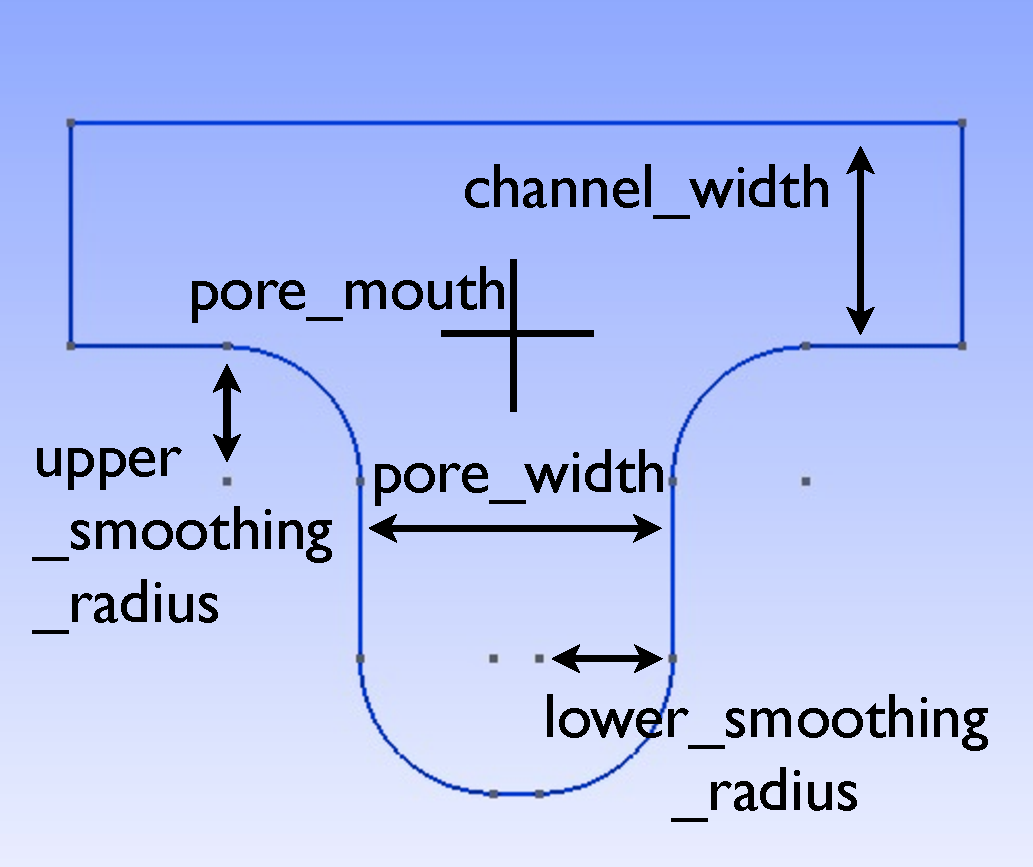
\includegraphics[height=6cm]{figures/slitpore.pdf}
  \caption{The slitpore created by the \codebox{constraint slitpore.}}
  \end{center}
\end{figure}

Variant \variant{8} specifies an electrostatic interaction between the
charged particles in the system to an infinitely long rod with a line
charge of \var{lambda} which is alinge along the z-axis and centered
at \var{c_x} and \var{c_y}.

Variant \variant{9} specifies the electrostatic interactinos between
the charged particles in the system and an inifinitely large plate in
the x-y-plane at height \var{h}. The plate carries a charge density of
\var{sigma}.
  
Variant \variant{10} specifies the dipolar coupling of particles with a
dipolar moment to an external field \var{f_x} \var{f_y} \var{f_z}.

Variant \variant{11} creates an infinite plane at a fixed position. For
non-initializing a direction of the constraint values of the positions
have to be negative. For the tunable-slip boundary interactions you
have to set \emph{two} constraints.

Variant \variant{14} creates a hollow-cone shaped boundary. The position can be any point in the simulation
box, and the orientation of the (cylindrically symmetric) cone is
given by a vector, which points in the direction of the symmetry axis, it
does not need to be normalized. The parameters: outer_radius \var{Ro},
inner_radius \var{Ri}, width \var{w}, and opening_angle \var{alpha}, specify the shape of the object. The inner radius gives the narrow end opening size, the outer radius the length of the shaft, and the width the layer width, i.e., the thickness of the cone. The opening_angle (between 0 and $\pi/2$) specifies the angle of the cone. 

Variant \variant{15} creates a spherocylinder, that is, a cylinder capped by a hemisphere on either side. The parameter length \var{length} specifies the length of the shaft, excluding the two hemispherical caps. 

Variant \variant{16} calculates the smallest distance to all non-penetrable
constraints, that can be repulsive (wall, cylinder, sphere, rhomboid, maze, pore, slitpore).
Negative distances mean that the position is ``within'' the area that
particles should not access. Helpful to find initial configurations.) 

\minisec{Example}
To create an infinite plane in $z$-direction at $z=20.0$ of type id 1,
use:
\begin{code}
  constraint plane cell -10 -10 20 type 1
\end{code}

\subsection{Deleting a constraint}
\begin{essyntax}
  constraint delete \opt{\var{num}} 
\end{essyntax}

This command will delete constraints. If \var{num} is specified only this
constraint will deleted, otherwise all constraints will be removed from the
system. 

\subsection{Getting the force on a constraint}
\begin{essyntax}
constraint force \var{n} 
\end{essyntax}
Returns the force acting on the \var{n}th constraint. Note, however, that this
are only forces due to interactions with particles, not with other constraints.
Also, these forces still do not mean that the constraints move, they are just
the negative of the sum of forces acting on all particles due to this constraint.
Similarly, the total energy does not containt constraint-constraint contributions.


\subsection{Getting the currently defined constraints}
\begin{essyntax}
constraint  \opt{\var{num}} 
\end{essyntax}
Prints out all constraint information. If \var{num} is specified only this
constraint is displayed, otherwise all constraints will be printed.

\subsection{\texttt{harmonic_well}: Creating a harmonic trap}
 \newescommand{harmonic-well}
 \begin{essyntax}
   harmonic_well \{ \var{x} \var{y} \var{z} \} \var{k}
  \begin{features}
    \required{CUDA}
  \end{features}
 \end{essyntax}

 Calculates a spring force for all particles, where the equilibrium position
 of the spring is at \var{x y z} and it's force constant is \var{k}. A more
 flexible trap can be constructed with constraints, but this one runs on the GPU.

\section{Virtual sites}
\label{sec:virtual}
\index{virtual sites|mainindex}

Virtual sites are particles, the positions and velocities of which are
not obtained by integrating an equation of motion.  Rather, their
coordinates are obtained from the position (and orientation) of one or
more other particles. In this way, rigid arrangements of particles can
be constructed and a particle can be placed in the center of mass of a
set of other particles.  Virtual sites can interact with other
particles in the system by means of interactions. Forces are added to
them according to their respective particle type. Before the next
integration step, the forces accumulated on a virtual site are
distributed back to those particles, from which the virtual site was
derived.

There are two distinct types of virtual sites, described in the
following.

\subsection{Virtual sites in the center of mass of a molecule}

To activate this implementation, enable the feature
\feature{VIRTUAL_SITES_COM} (sec. \ref{sec:myconfig}).  Virtual sites
are then placed in the center of mass of a set of particles (as
defined below). Their velocity will also be that of the center of
mass. Forces accumulating on the virtual sites are distributed back to
the particles which form the molecule.  To place a virtual site at the
center of a molecule, perform the following steps in that order
\begin{enumerate}
\item Create a particle of the desired type for each molecule. It
  should be placed at least roughly in the center of the molecule to
  make sure, it's on the same node as the other particles forming the
  molecule, in a simulation with more than one cpu.
\item Make it a virtual site using 
  \begin{essyntaxbox}
    part \var{pid} virtual 1
  \end{essyntaxbox}
\item Declare the list of molecules and the particles they consist of:
  \begin{essyntaxbox}
    analyze set \{\var{moltype} \var{list of particle ids} ...\} ...
  \end{essyntaxbox}
  The lists of particles in a molecule comprise the non-virtual
  particles as well as the virtual site. The id of this molecule is
  its index in this list. For example,
  \begin{code}
    analyze set \{0 1 2 3 4\} \{0 5 6 7 8\} \{1 9 10 11\}
  \end{code}
  declares three molecules, of which the first two consist of three
  particles and a virtual site each (particles 1--4 and 5--8,
  respectively). The third molecule has type 1 and consists of two
  particles and a virtual site. The virtual sites were determined
  before by setting the \var{virtual} flag. You can choose freely one
  out of each molecule, for example particles 1, 5, and 9.
\item Assign to all particles that belong to the same molecule the
  molecule's id
  \begin{essyntaxbox}
    part \var{pid} mol \var{molid}
  \end{essyntaxbox}
  The molid is the index of the particle in the above list, so you
  would assign \var{molid} 0 to particles 1-4, \var{molid} 1 to
  particles 5-8 and \var{molid} 2 to particles 9-11. Alternatively,
  you can call
  \begin{essyntaxbox}
    analyze set topo_part_sync
  \end{essyntaxbox}
  to set the \var{molid}s from the molecule declarations.
\item Update the position of all virtual particles (optional)
  \begin{essyntaxbox}
    integrate 0
  \end{essyntaxbox}
\end{enumerate}
Please note that the use of virtual sites requires that the particles are numbered consecutively. I.e., the particle ids should go from zero to $N-1$, where $N$ is the number of particles.

The type of the molecule you can choose freely, it is only used in
certain analysis functions, namely \texttt{energy_kinetic_mol},
\texttt{pressure_mol} and \texttt{dipmom_mol}, which compute kinetic
energy, pressure and dipole moment per molecule type, respectively.


\subsection{Rigid arrangements of particles}

The ``relative'' implementation of virtual sites allows for the
simulation of rigid arrangements of particles. It can be used, \eg,
for extended dipoles and raspberry-particles, but also for more
complex configurations.  Position and velocity of a virtual site are
obtained from the position and orientation of exactly one non-virtual
particle, which has to be placed in the center of mass of the rigid
body. Several virtual sites can be related to one and the same
non-virtual particle.  The position of the virtual site is given by
\begin{equation}
\vec{x_v} =\vec{x_n} +O_n (O_v \vec{E_z}) d,
\end{equation}
where $\vec{x_n}$ is the position of the non-virtual particle, $O_n$
is the orientation of the non-virtual particle, $O_v$ denotes the
orientation of the vector $\vec{x_v}-\vec{x_n}$ with respect to the
non-virtual particle's body fixed frame and $d$ the distance between
virtual and non-virtual particle.  In words: The virtual site is
placed at a fixed distance from the non-virtual particle. When the
non-virtual particle rotates, the virtual sites rotates on an orbit
around the non-virtual particle's center.

To use this implementation of virtual sites, activate the feature
\feature{VIRTUAL_SITES_RELATIVE} (see sec. \ref{sec:myconfig}).  To
set up a virtual site,
\begin{enumerate}
\item Place the particle to which the virtual site should be
  related. It needs to be in the center of mass of the rigid
  arrangement of particles you create. Let its particle id be n.
\item Place a particle at the desired relative position, make it
  virtual and relate it to the first particle
  \begin{essyntaxbox}
    part \var{v} pos \var{pos} virtual 1 vs_auto_relate \var{n}
  \end{essyntaxbox}
\item Repeat the previous step with more virtual sites, if desired.
\item To update the positions of all virtual sites, call
  \begin{essyntaxbox}
    integrate 0
  \end{essyntaxbox}
\end{enumerate}

Please note:
\begin{itemize}
\item The relative position of the virtual site is defined by its
  distance from the non-virtual particle, the id of the non-virtual
  particle and a quaternion which defines the vector from non-virtual
  particle to virtual site in the non-virtual particle's body-fixed
  frame. This information is saved in the virtual site's
  vs\_relative-attribute. Take care, not to overwrite these after using
  vs\_auto\_relate.
\item Virtual sites can not be placed relative to other virtual sites,
  as the order in which the positions of virtual sites are updated is
  not guaranteed. Always relate a virtual site to a non-virtual
  particle placed in the center of mass of the rigid arrangement of
  particles.
\item Don't forget to declare the particle virtual in addition to
  calling vs\_auto\_relate
\item In case you know the correct quaternions, you can also setup a
  virtual site using
  \begin{essyntaxbox}
    part \var{v} virtual 1 vs_relative \var{n} \var{d} \var{q}
  \end{essyntaxbox}
  where n is the id of the non-virtual particle, d is its distance
  from the virtual site, and q are the quaternions.
\item In a simulation on more than one CPU, the effective cell size
  needs to be larger than the largest distance between a non-virtual
  particle and its associated virtual sites. To this aim, you need to
  set the global variable \var{min\_global\_cut} to this largest
  distance. \es issues a warning when creating a virtual site with
  \lit{vs_auto_relate_to} and the cutoff is insufficient.
\item If the virtual sites represent actual particles carrying a mass,
  the inertia tensor of the non-virtual particle in the center of mass
  needs to be adapted.
\item The presence of rigid bodies constructed by means of virtual
  sites adds a contribution to the pressure and stress tensor.
\item The use of virtual sites requires that the particles are
  numbered consecutively, \ie, the particle ids should go from zero to
  $N-1$, where $N$ is the number of particles.
\end{itemize}

\subsection{Additional features}

The behaviour of virtual sites can be fine-tuned with the following
switches in \texttt{myconfig.hpp} (sec. \ref{sec:myconfig})
\begin{itemize}
\item \feature{VIRTUAL_SITES_NO_VELOCITY} specifies that the velocity
  of virtual sites is not computed
\item \feature{VIRTUAL_SITES_THERMOSTAT} specifies that the Langevin
  thermostat should also act on virtual sites
\item \feature{THERMOSTAT_IGNORE_NON_VIRTUAL} specifies that the
  thermostat does not act on non-virtual particles
\end{itemize}

\section{Grand canonical feature}
For using \es conveniently for simulations in the grand canonical ensemble, or
other purposes, when particles of certain types are created and deleted frequently.
Particle ids can be stored in lists for each individual type and so random ids of
particles of a certain type can be drawn. 

\begin{essyntax}
part gc
\alt{\var{type} \asep \alt{\alt{find \asep delete \asep
status \asep number} \var{type}}}
\end{essyntax}

If you want \es to keep track of particle ids of a certain type you have to
initialize the method by calling 
\begin{essyntax}
	part gc \var{type}
\end{essyntax}
After that \es will keep track of particle ids of that type. 
When using the keyword \texttt{find} and a particle type, the
command will return a randomly chosen particle id, for a particle of
the given type. 
The keyword \texttt{status} will return a list with all particles with the given
type, similarly giving \texttt{number} as argument will return the number of
particles which share the given type.

%%% Local Variables: 
%%% mode: latex
%%% TeX-master: "ug"
%%% End: 

% Copyright (C) 2010,2011,2012,2013,2014 The ESPResSo project
% Copyright (C) 2002,2003,2004,2005,2006,2007,2008,2009,2010 
%   Max-Planck-Institute for Polymer Research, Theory Group
%  
% This file is part of ESPResSo.
%   
% ESPResSo is free software: you can redistribute it and/or modify it
% under the terms of the GNU General Public License as published by the
% Free Software Foundation, either version 3 of the License, or (at your
% option) any later version.
%  
% ESPResSo is distributed in the hope that it will be useful, but
% WITHOUT ANY WARRANTY; without even the implied warranty of
% MERCHANTABILITY or FITNESS FOR A PARTICULAR PURPOSE.  See the GNU
% General Public License for more details.
%  
% You should have received a copy of the GNU General Public License
% along with this program.  If not, see <http://www.gnu.org/licenses/>.
%
\chapter{Setting up interactions}
\label{sec:inter}
\newescommand{inter}
\index{interactions|mainindex}

In \es, interactions are set up and investigated by the
\keyword{inter} command. There are mainly two types of interactions:
non-bonded and bonded interactions. Non-bonded interactions only
depend on the \emph{type} of the two involved particles. This also
applies to the electrostatic interaction; however, due to its
long-ranged nature, it requires special care and \es handles it
separately with a number of state-of-the-art algorithms. The particle
type and the charge are both defined using the \lit{part} command.

A bonded interaction defines an interaction between a number of
specific particles; it only applies to the set of particles for which
it has been explicitely set.  A bonded interaction between a set of
particles has to be specified explicitely by the \lit{part bond}
command, while the \lit{inter} command is used to define the
interaction parameters.

\begin{essyntax}
  inter
\end{essyntax}
Without any arguments, \lit{inter} returns a list of all defined
interactions as a Tcl-list. The format of each entry corresponds to
the syntax for defining the interaction as described below. Typically,
this list looks like
\begin{tclcode}
  {0 0 lennard-jones 1.0 2.0 1.1225 0.0 0.0} {0 FENE 7.0 2.0}
\end{tclcode}


\section{Isotropic non-bonded interactions}
\label{sec:inter-nb}
\index{Non-bonded interactions|mainindex}
\index{interactions!non-bonded|mainindex}

\begin{essyntax*}
  inter \var{type1} 
  \var{type2}
  \opt{\var{interaction}}
  \opt{\var{parameters}}
\end{essyntax*}
This command defines an interaction of type \var{interaction} between
all particles of type \var{type1} and \var{type2}. The possible
interaction types and their parameters are listed below. If the
interaction is omitted, the command returns the currently defined
interaction between the two types using the syntax to define the
interaction, \eg
\begin{tclcode}
  0 0 lennard-jones 1.0 2.0 1.1225 0.0 0.0
\end{tclcode}

For many non-bonded interactions, it is possible to artificially cap
the forces, which often allows to equilibrate the system much
faster. See the subsection~\ref{sec:forcecap} for details.


\subsection{Tabulated interaction}
\index{tabulated interaction|mainindex}
\index{interactions!tabulated|mainindex}
\label{sec:tabnonbonded}

\begin{essyntax}
  inter \var{type1} \var{type2} tabulated \var{filename}%
  \begin{features}
    \required{TABULATED}
  \end{features}
\end{essyntax}

This defines an interaction between particles of the types \var{type1} and
\var{type2} according to an arbitrary tabulated pair potential. \var{filename}
specifies a file which contains the tabulated forces and energies as a function
of the separation distance. The tabulated potential allows capping the force
using \lit{inter forcecap}, see section~\ref{sec:forcecap}.

At present the required file format is simply an ordered list separated by
whitespace. The data reader first looks for a {\tt \#} character and begins
reading from that point in the file. Anything before the {\tt \#} will be
ignored.

The first three parameters after the {\tt \#} specify the number of data points
$N_\mathrm{points}$ and the minimal and maximal tabulated separation distances
$r_\mathrm{min}$ and $r_\mathrm{max}$. The number of data points obviously should
be an integer, the two other can be arbitrary positive doubles. Take care when
choosing the number of points, since a copy of each lookup table is kept on each
node and must be referenced very frequently. The maximal tabulated separation
distance also acts as the effective cutoff value for the potential.

The remaining data in the file should consist of n data triples $r$, $F(r)$ and
$V(r)$. $r$ gives the particle separation, $V(r)$ specifies the interaction
potential, and $F(r)= -V'(r)/r$ the force (note the factor $1/r$!). The values
of $r$ are assumed to be equally distributed between $r_\mathrm{min}$ and
$r_\mathrm{max}$ with a fixed distance of
$(r_\mathrm{max}-r_\mathrm{min})/(N_\mathrm{points}-1)$; the distance values $r$ in
the file are ignored and only included for human readability.

\subsection{Lennard-Jones interaction}
\label{sec:LennardJones}

\index{Lennard-Jones interaction|mainindex}
\index{interactions!Lennard-Jones|mainindex}
\begin{essyntax}
  inter \var{type1} 
  \var{type2}
  lennard-jones 
  \var{\epsilon} \var{\sigma} 
  \var{r_\mathrm{cut}} 
  \opt{\alt{\var{c_\mathrm{shift}}|auto}
    \opt{\var{r_\mathrm{off}}
      \opt{\var{r_\mathrm{cap}} 
        \opt{ \var{r_\mathrm{min}}}}}}
  \begin{features}
    \required{LENNARD_JONES}
  \end{features}
\end{essyntax}

This command defines the traditional (12-6)-Lennard-Jones interaction
between particles of the types \var{type1} and \var{type2}.  The
potential is defined by
\begin{equation}
  \label{eq:lj}
  V_\mathrm{LJ}(r) = \Biggl\{
    \begin{array}{ll}
      4\epsilon((\frac{\var{\sigma}}{r-\var{r_\mathrm{off}}})^{12}
      - (\frac{\var{\sigma}}{r-\var{r_\mathrm{off}}})^6+\var{c_\mathrm{shift}}) 
      & \mathrm{, if~} \var{r_\mathrm{min}}+\var{r_\mathrm{off}} < \var{r} < \var{r_\mathrm{cut}}+\var{r_\mathrm{off}}\\
      \mathit{0} 
      & \mathrm{, otherwise}\\
    \end{array}.
\end{equation}

The traditional Lennard--Jones potential is the ``work--horse''
potential of particle--particle interactions in coarse--grained
simulations.  It is a simple model of the van--der--Waals interaction,
and is attractive at large distance, but strongly repulsive at short
distances.  $\var{r_\mathrm{off}} + \var{\sigma}$ corresponds to the
sum of the radii of the interaction particles; at this radius,
$V_\mathrm{LJ}(\var{r}) = 4 \var{\epsilon} \var{c_\mathrm{shift}}$.
The minimum of the potential is at $\var{r} = \var{r_\mathrm{off}} +
2^\frac{1}{6}\var{\sigma}$.  At this value of $r$, $V_\mathrm{LJ}(r) =
-\var{\epsilon} + 4 \var{\epsilon} \var{c_\mathrm{shift}}$. The
attractive part starts beyond this value of $\var{r}$.
$\var{r_\mathrm{cut}}$ determines the radius where the potential is
cut off. 

If \var{c_\mathrm{shift}} is not set or it is set to the string
\lit{auto}, the shift will be automatically computed such that the
potential is continuous at the cutoff radius. If \var{r_\mathrm{off}}
is not set, it is set to $0$.

The total force on a particle can be capped by using the command
\lit{inter forcecap}, see section~\ref{sec:forcecap}, or on an
individual level using the \var{r_\mathrm{cap}} variable. When
\var{r_\mathrm{cap}} is set \emph{and} \lit{inter forcecap
  individual} has been issued before, the maximal force that is generated by
this potential is the force at \var{r_\mathrm{cap}}.  By default,
force capping is off, \ie the cap radius is set to 0.

An optional additional parameter can be used to restrict the
interaction from a \emph{minimal} distance
$\var{r_\mathrm{min}}$. This is an optional parameter, set to 0 by
default.

A special case of the Lennard--Jones potential is the
Weeks--Chandler--Andersen (WCA) potential, which one obtains by
putting the cutoff into the minimum, \ie choosing
$\var{r_\mathrm{cut}}=2^\frac{1}{6}\var{\sigma}$. The WCA potential is
purely repulsive, and is often used to mimick hard sphere repulsion.


When coupling particles to a Shan-Chen fluid, if the \lit{affinity} interaction is set, the Lennard-Jones potential is multiplied by the function 

\begin{equation}
  \label{eq:lj-affinity}
  A(r) = \Biggl\{
    \begin{array}{ll}
      \frac{(1-\alpha_1)}{2} [1+\tanh(2\phi)]  +  \frac{(1-\alpha_2)}{2} [1+\tanh(-2\phi)]
      & \mathrm{, if~}  \var{r} > \var{r_\mathrm{cut}}+2^{\frac{1}{6}}\sigma\\
      1
      & \mathrm{, otherwise~} \\
    \end{array},
\end{equation}
where $\alpha_i$ is the affinity to the $i$-th fluid component (see
\ref{sec:affinity}), and the order parameter $\phi$ is calculated
from the fluid component local density as $\phi=\frac{\rho_1 -
\rho_2}{\rho_1+\rho_2}$. For example, if the affinities are chosen
so that the first component is a good solvent ($\alpha_1=1$) and
the second one is a bad solvent ($\alpha_2=0$), then, if the two
particles are both in a region rich in the first component, then
$\phi\simeq1$, and $A(r)\simeq0$ for
$r>\var{r_\mathrm{cut}}+2^{\frac{1}{6}}\sigma$.  Therefore, the
interaction potential will be very close to the WCA one. Conversely,
if both particles are in a region rich in the second component,
then $\phi\simeq-1$, and  $A(r)\simeq 1$, so that the potential
will be very close to the full LJ one. If the cutoff has been set
large enough, the particle will experience the attractive part of
the potential, mimiking the effective attraction induced by the bad
solvent.



\subsection{Generic Lennard-Jones interaction}
\index{Generic Lennard-Jones interaction|mainindex}
\index{interactions!Generic Lennard-Jones|mainindex}
\label{sec:GenLennardJones}

\begin{essyntax}
  inter \var{type1} 
  \var{type2}
  lj-gen
  \var{\epsilon} \var{\sigma} 
  \var{r_\mathrm{cut}} \var{c_\mathrm{shift}} \var{r_\mathrm{off}}
  \var{e_1} \var{e_2} \var{b_1} \var{b_2}
  \opt{\alt{\var{r_\mathrm{cap}}|auto} \var{\lambda} \var{\delta}}
  \begin{features}
    \required{LENNARD_JONES_GENERIC}
  \end{features}
\end{essyntax}

This command defines a generalized version of the Lennard-Jones
interaction (see section \ref{sec:LennardJones}) between particles of
the types \var{type1} and \var{type2}.  The potential is defined by
\begin{equation}
  \label{eq:lj-generic}
  V_\mathrm{LJ}(r) = \Biggl\{
    \begin{array}{ll}
      \epsilon(\var{b_1}(\frac{\var{\sigma}}{r-\var{r_\mathrm{off}}})^\var{e_1}
      -\var{b_2}(\frac{\var{\sigma}}{r-\var{r_\mathrm{off}}})^{e_2}+\var{c_\mathrm{shift}}) 
      & \mathrm{, if~} \var{r_\mathrm{min}}+\var{r_\mathrm{off}} < \var{r} < \var{r_\mathrm{cut}}+\var{r_\mathrm{off}}\\
      \mathit{0} 
      & \mathrm{, otherwise}\\
    \end{array}.
\end{equation}
Note that the prefactor 4 of the standard LJ potential is missing, so the normal
LJ potential is recovered for $b_1=b_2=4$, $e_1=12$ and $e_2=6$.

The total force on a particle can be capped by using the command
\lit{inter forcecap}, see section~\ref{sec:forcecap}, or on an
individual level using the \var{r_\mathrm{cap}} variable. When
\var{r_\mathrm{cap}} is set \emph{and} \lit{inter forcecap
  individual} has been issued before, the maximal force that is generated by
this potential is the force at \var{r_\mathrm{cap}}.  By default,
force capping is off, \ie the cap radius is set to 0.

The optional \texttt{LJGEN_SOFTCORE} feature activates a softcore version 
of the potential, where the following transformations apply: 
$\epsilon \rightarrow \lambda \epsilon$
and
$r-\var{r_\mathrm{off}} \rightarrow \sqrt{(r-\var{r_\mathrm{off}})^2 -
(1-\lambda) \delta \sigma^2}$. \var{\lambda} allows to tune the strength 
of the interaction, while \var{\delta} varies how smoothly the potential
goes to zero as $\var{\lambda}\rightarrow 0$. Such a feature allows one to
perform alchemical transformations, where a group of atoms can be slowly
turned on/off during a simulation.

\subsection{Lennard-Jones cosine interaction}
\index{Lennard-Jones cosine interaction|mainindex}
\index{interactions!Lennard-Jones cosine|mainindex}
\begin{essyntax}
  \variant{1}
  inter \var{type1} \var{type2} lj-cos
  \var{\epsilon} \var{\sigma}
  \var{r_\mathrm{cut}} \var{r_\mathrm{off}}
  \variant{2}
  inter \var{type1} \var{type2} lj-cos2
  \var{\epsilon} \var{\sigma} 
  \var{r_\mathrm{off}} \var{\omega}
  \begin{features}
    \required[\variant{1}]{LJCOS}
    \required[\variant{2}]{LJCOS2}
  \end{features}
\end{essyntax}
specifies a Lennard-Jones interaction with cosine
tail~\cite{soddeman01a} between particles of the types \var{type1} and
\var{type2}. The first variant behaves as follows: Until the minimum
of the Lennard-Jones potential at $\var{r_\mathrm{min}} = r_\mathrm{off} +
2^{\frac{1}{6}}\sigma$, it behaves identical to the unshifted
Lennard-Jones potential ($\var{c_\mathrm{shift}}=0$).  Between
\var{r_\mathrm{min}} and \var{r_\mathrm{cut}}, a cosine is used to
smoothly connect the potential to 0, \ie
\begin{equation}
  V(r)=\frac{1}{2}\epsilon\left(cos\left[\alpha(\var{r}-\var{r_\mathrm{off}})^2 + \beta\right]-1\right),
\end{equation}
where
$\alpha = \pi\left[(\var{r_\mathrm{cut}}-\var{r_\mathrm{off}})^2-(\var{r_\mathrm{min}}-\var{r_\mathrm{off}})^2\right]^{-1}$
and
$\beta = \pi - \left(\var{r_\mathrm{min}}-\var{r_\mathrm{off}}\right)^2\alpha$.

In the second variant, the cutoff radius is
$\var{r_\mathrm{cut}}=\var{r_\mathrm{min}} + \omega$, where $\var{r_\mathrm{min}} =  r_\mathrm{off} +
2^{\frac{1}{6}}\sigma$ as in the first variant. The potential
between $\var{r_\mathrm{min}}$ and $\var{r_\mathrm{cut}}$ is given by
\begin{equation}
  V(r)=\epsilon\cos^2\left[\frac{\pi}{2\omega}(\var{r} - \var{r_\mathrm{min}})\right].
\end{equation}
For $\var{r} < \var{r_\mathrm{min}}$, $V(r)$ is implemented as normal
Lennard-Jones potential, see equation \ref{eq:lj} with
$\var{c_\mathrm{shift}} = 0$.

Only the second variant allows capping the force using \lit{inter
  forcecap}, see section~\ref{sec:forcecap}.

\subsection{Smooth step interaction}
\index{smooth-step interaction|mainindex}
\index{interactions!smooth-step|mainindex}
\begin{essyntax}
  inter \var{type1} \var{type2}
  smooth-step \var{\sigma_1} \var{n} \var{\epsilon} \var{k_0}
  \var{\sigma_2} \var{r_\mathrm{cut}}
  \begin{features}
    \required{SMOOTH_STEP}
  \end{features}
\end{essyntax}
This defines a smooth step interaction between particles of the
types \var{type1} and \var{type2}, for which the potential is
\begin{equation}
  V(r)= \left(\var{\sigma_1}/d\right)^\var{n} + \epsilon/(1 + \exp\left[2k_0 (r - \sigma_2)\right])
\end{equation}
for $r<r_\mathrm{\var{cut}}$, and $V(r)=0$ elsewhere. With $n$ around
10, the first term creates a short range repulsion similar to the
Lennard-Jones potential, while the second term provides a much softer
repulsion. This potential therefore introduces two length scales, the
range of the first term, $\sigma_1$, and the range of the second one,
$\sigma_2$, where in general $\sigma_1<\sigma_2$.

\subsection{BMHTF potential}
\index{BMHTF interaction|mainindex}
\index{interactions!BMHTF|mainindex}
\begin{essyntax}
  inter \var{type1} \var{type2}
  bmhtf-nacl \var{A} \var{B} \var{C} \var{D} \var{\sigma} \var{r_\mathrm{cut}}
  \begin{features}
    \required{BMHTF_NACL}
  \end{features}
\end{essyntax}
This defines an interaction with the {\em short-ranged part} of the
Born-Meyer-Huggins-Tosi-Fumi potential between particles of the types
\var{type1} and \var{type2}, which is often used to simulate NaCl
crystals. The potential is defined by:
\begin{equation}
  V(r)= \var{A}\exp\left[\var{B}(\var{\sigma} - \var{r})\right] -
  \var{C} \var{r}^{-6} - \var{D} \var{r}^{-8} + \epsilon_\mathrm{shift},
\end{equation}
where $\epsilon_\mathrm{shift}$ is chosen such that
$V(\var{r_\mathrm{cut}})=0$. For $r\ge \var{r_\mathrm{cut}}$, the
$V(r)=0$.

For NaCl, the parameters should be chosen as follows:

\begin{tabular}{r|l|l|l|l|l}
  types & \var{A} (\unitfrac{kJ}{mol}) & \var{B} ($\unit{\AA^{-1}}$) &
  \var{C} ($\unit{\AA^6}$\unitfrac{kJ}{mol}) & \var{D}
  $\unit{\AA^8}$\unitfrac{kJ}{mol} & \var{\sigma} (\unit{\AA}) \\
  \hline
  Na-Na & 25.4435 & 3.1546 &  101.1719 &    48.1771 & 2.34 \\
  Na-Cl & 20.3548 & 3.1546 &  674.4793 &   837.0770 & 2.755 \\
  Cl-Cl & 15.2661 & 3.1546 & 6985.6786 & 14031.5785 & 3.170 \\
\end{tabular}

The cutoff can be chosen relatively freely because the potential
decays fast; a value around 10 seems reasonable.

In addition to this short ranged interaction, one needs to add a
Coulombic, long--ranged part. If one uses elementary charges, \ie a
charge of $q=+1$ for the Na--particles, and $q=-1$ for the
Cl--particles, the corresponding prefactor of the Coulomb interaction
is $\approx 1389.3549 \AA\,kJ/mol$.

\subsection{Morse interaction}
\index{Morse interaction|mainindex}
\index{interactions!Morse|mainindex}

\begin{essyntax}
  inter \var{type1} \var{type2} morse
  \var{\epsilon} \var{\alpha} \var{r_\mathrm{min}} \var{r_\mathrm{cut}}
  \begin{features}
    \required{MORSE}
  \end{features}
\end{essyntax}
This defines an interaction using the Morse potential between
particles of the types \var{type1} and \var{type2}. It serves similar
purposes as the Lennard-Jones potential, but has a deeper minimum,
around which it is harmonic.  This models the potential energy in a
diatomic molecule.  This potential allows capping the force using
\texttt{inter forcecap}, see section~\ref{sec:forcecap}.

For $r < \var{r_\mathrm{cut}}$, this potential is given by
\begin{equation}
  V(r)=\var{\epsilon}\left(\exp\left[-2 \var{\alpha} \left(r - \var{r_\mathrm{min}}\right)\right]
    - 2\exp\left[-\alpha\left(r - r_\mathrm{min}\right)\right]\right) -
  \epsilon_\mathrm{shift},
\end{equation}
where \var{\epsilon_\mathrm{shift}} is again chosen such that
$V(\var{r_\mathrm{cut}})=0$. For $r\ge \var{r_\mathrm{cut}}$, the $V(r)=0$.

\subsection{Buckingham interaction}
\index{Buckingham interaction|mainindex}
\index{interactions!Buckingham|mainindex}

\begin{essyntax}
  inter \var{type1} \var{type2} buckingham
  \var{A} \var{B} \var{C} \var{D}
  \var{r_\mathrm{cut}} \var{r_\mathrm{discont}} \var{\epsilon_\mathrm{shift}}
  \begin{features}
    \required{BUCKINGHAM}
  \end{features}
\end{essyntax}
This defines a Buckingham interaction between particles of the types
\var{type1} and \var{type2}, for which the potential is given by
\begin{equation}
  V(r)= A\exp(-B r) - Cr^{-6} - Dr^{-4} + \var{\epsilon_\mathrm{shift}}
\end{equation}
for $\var{r_\mathrm{discont}} < r < \var{r_\mathrm{cut}}$. Below \var{r_\mathrm{discont}},
the potential is linearly continued towards $r=0$, similarly to force capping,
see below. Above $r=\var{r_\mathrm{cut}}$, the potential is $0$. This potential
allows capping the force using \lit{inter forcecap}, see
section~\ref{sec:forcecap}.

\subsection{Soft-sphere interaction}
\index{soft-sphere interaction|mainindex}
\index{interactions!soft-sphere|mainindex}

\begin{essyntax}
  inter \var{type1} \var{type2}
  soft-sphere \var{a} \var{n} \var{r_\mathrm{cut}} \var{r_\mathrm{offset}}
  \begin{features}
    \required{SOFT_SPHERE}
  \end{features}
\end{essyntax}
This defines a soft sphere interaction between particles of the types
\var{type1} and \var{type2}, which is defined by a single power law:
\begin{equation}
  V(r)=a\left(r-r_\mathrm{\var{offset}}\right)^{-n}
\end{equation}
for $r<\var{r_\mathrm{cut}}$, and $V(r)=0$ above. There is no shift
implemented currently, which means that the potential is discontinuous
at $r=\var{r_\mathrm{cut}}$. Therefore energy calculations should be
used with great caution.

\subsection{Hat interaction}
\index{hat interaction|mainindex}
\index{interactions!hat|mainindex}

\begin{essyntax}
  inter \var{type1} \var{type2}
  hat \var{F_\text{max}} \var{r_c}
  \begin{features}
    \required{HAT}
  \end{features}
\end{essyntax}
This defines a simple force ramp between particles of the types \var{type1} and
 \var{type2}. The maximal force \var{F_\text{max}} acts at zero distance and 
zero force is applied at distances $r_c$ and bigger. For distances smaller than 
\var{r_c}, the force is given by
\begin{equation}
  F(r)=F_{\text{max}} \cdot \left( 1 - \frac{r}{r_c} \right),
\end{equation}
for distances exceeding \var{r_c}, the force is zero.

The potential energy is given by
\begin{equation}
  V(r)=F_{\text{max}} \cdot (r-r_c) \cdot \left( \frac{r+r_c}{2r_c} - 1 \right),
\end{equation}
which is zero for distances bigger than \var{r_c} and continuous at distance 
\var{r_c}.

This is the standard conservative DPD potential and can be used in combination 
with \lit{inter DPD} \ref{sec:DPDinter}. The potential is also useful for live 
demonstrations, where a big time step may be employed to obtain quick results
on a weak machine, for which the physics do not need to be entirely correct.  

\subsection{Hertzian interaction}
\index{Hertzian interaction|mainindex}
\index{interactions!hertzian|mainindex}

\begin{essyntax}
  inter \var{type1} \var{type2}
  hertzian \var{\sigma} \var{\epsilon}
  \begin{features}
    \required{HERTZIAN}
  \end{features}
\end{essyntax}
This defines an interaction according to the Hertzian potential
between particles of the types \var{type1} and \var{type2}. The
Hertzian potential is defined by
\begin{equation}
  V(r)=
  \begin{cases} \epsilon\left(1-\frac{r}{\sigma}\right)^{5/2} & r < \sigma\\
    0 & r \ge \sigma.
  \end{cases}
\end{equation}
The potential has no singularity and is defined everywhere; the
potential has nondifferentiable maximum at $r=0$, where the force is
undefined.

\subsection{Gaussian}
\index{Gaussian interaction|mainindex}
\index{interactions!gaussian|mainindex}

\begin{essyntax}
  inter \var{type1} \var{type2}
  gaussian \var{\sigma} \var{\epsilon} \var{r_\mathrm{cut}}
  \begin{features}
    \required{GAUSSIAN}
  \end{features}
\end{essyntax}
This defines an interaction according to the Gaussian potential 
between particles of the typers \var{type1} and \var{type2}.  The
Gaussian potential is defined by
\begin{equation}
  V(r) = 
  \begin{cases} \epsilon\,e^{-\frac{1}{2}\left(\frac{r}{\sigma}\right)^{2}}
    & r < \var{r_\mathrm{cut}}\\
  0 & r \ge \var{r_\mathrm{cut}}
  \end{cases}
\end{equation}
The Gaussian potential is smooth except at the cutoff, and has a
finite overlap energy of $\epsilon$. It can be used to model \eg{}
overlapping polymer coils. 

Currently, there is no shift implemented, which means that the potential 
is discontinuous at $r=\var{r_\mathrm{cut}}$.  Therefore use caution when 
performing energy calculations. However, you can often choose the
cutoff such that the energy difference at the cutoff is less than a
desired accuracy, since the potential decays very
rapidly.

\section{Anisotropic non-bonded interactions}
\label{inter-anisotropic}
\index{Anisotropic interactions}

\subsection{Directional Lennard-Jones interaction}
\index{Directional Lennard-Jones interaction|mainindex}
\index{interactions!Directional Lennard-Jones|mainindex}
\begin{essyntax}
  inter \var{type1} \var{type2} lj-angle
  \var{\epsilon} \var{\sigma}
  \var{r_\mathrm{cut}} \var{b1_a} \var{b1_b}
  \var{b2_a} \var{b2_b} \opt{\var{r_\mathrm{cap}} 
    \var{z_0} \var{\delta z} \var{\kappa} \var{\epsilon'}}
  \begin{features}
    \required{LJ_ANGLE}
  \end{features}
\end{essyntax}

\begin{center}
  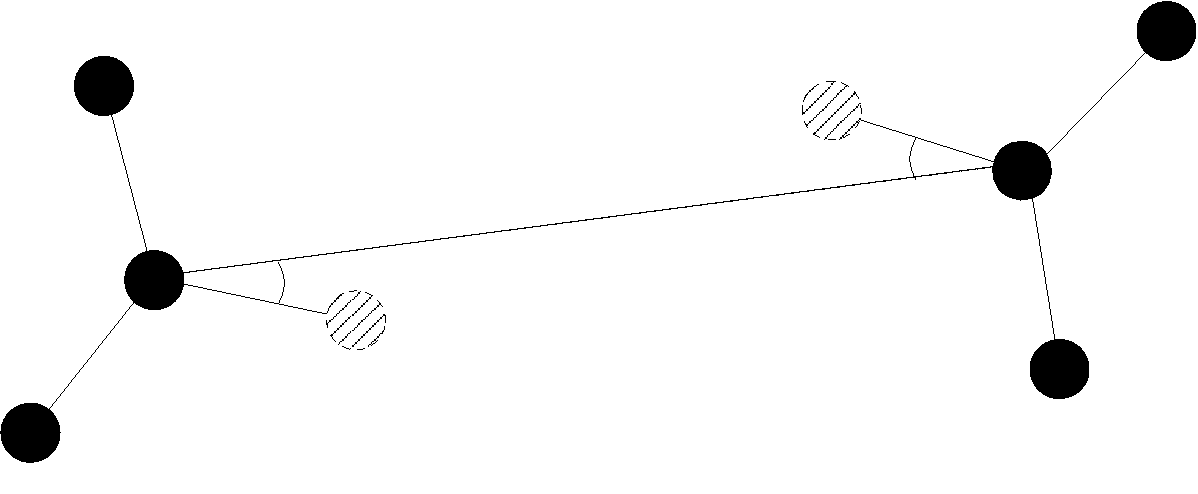
\includegraphics[height=8em]{figures/hbond}
\end{center}

Specifies a 12-10 Lennard-Jones interaction with angular dependence between
particles of the types \var{type1} and \var{type2}. These two particles need
two bonded partners oriented in a symmetric way. They define an orientation
for the central particle. The purpose of using bonded partners is to avoid
dealing with torques, therefore the interaction does \emph{not} need the
ROTATION feature. The angular part of the potential minimizes the system when
the two central beads are oriented along the vector formed by these two
particles. The shaded beads on the image are virtual particles that are formed
from the orientation of the bonded partners, connected to the central
beads. They are used to define angles. The potential is of the form
\begin{equation}
  U(r_{ik},\theta_{jik},\theta_{ikn})=
  \epsilon\left[5\left(\frac{\sigma}r\right)^{12} - 
    6\left(\frac{\sigma}{r}\right)^{10}\right]
  \cos^2\theta_{jik}\cos^2\theta_{ikn},
\end{equation}
where $r_{ik}$ is the distance between the two central beads, and each angle
defines the orientation between the direction of a central bead (determined
from the two bonded partners) and the vector $\mathbf{r_{ik}}$. Note that the
potential is turned off if one of the angle is more than $\pi/2$. This way we
don't end up creating a minimum for an anti-parallel configuration.

Unfortunately, the bonded partners are not seeked dynamically. One has to keep
track of the relative positions of the particle IDs. This can be done by
setting the parameters \var{b1_a}, \var{b1_b}, \var{b2_a}, and \var{b2_b}. Say
the first bead \var{type1} has particle ID \var{n}, then one should set the
simulation such as its two bonded partners have particle IDs \var{n+b1_a} and
\var{n+b1_b}, respectively. On a linear chain, for example, one would
typically have \var{b1_a=1} and \var{b1_b=-1} such that the central bead and
its two bonded partners have position IDs \var{n}, \var{n+1}, and \var{n-1},
respectively. This is surely not optimized, but once the simulation is set
correctly the algorithm is very fast.

The force can be capped using \lit{inter forcecap}. It might turn out
to be useful in some cases to keep this capping during the whole
simulation. This is due to the very sharp angular dependence for small
distance, compared to $\sigma$. Two beads might come very close to each other
while having unfavorable angles such that the interaction is turned off. Then
a change in the angle might suddenly turn on the interaction and the system
will blow up (the potential is so steep that one would need extremely small
time steps to deal with it, which is not very clever for such rare events).

For instance, when modeling hydrogen bonds (N-H...O=C), one can avoid
simulating hydrogens and oxygens by using this potential. This comes down to
implementing a HBond potential between N and C atoms.

The optional parameter \var{r_\mathrm{cap}} is the usual cap radius. The four
other optional parameters (\var{z_0}, \var{\delta z}, \var{\kappa},
\var{\epsilon'}) describe a different interaction strength \var{\epsilon'} for
a subset of the simulation box. The box is divided through the \var{z} plane
in two different regions: region 1 which creates an interaction with strength
\var{\epsilon}, region 2 with interaction strength \var{\epsilon'}. The 2nd
region is defined by its \var{z}-midplane \var{z_0}, its total thickness
\var{\delta z}, and the interface width \var{\kappa}. Therefore, the
interaction strength is \var{\epsilon} everywhere except for the region of the
box $z_0-\delta z/2<z<z_0+\delta z/2$. The interface width smoothly
interpolates between the two regions to avoid discontinuities. As an example,
one can think of modeling hydrogen bonds in two different environments: water,
where the interaction is rather weak, and in a lipid bilayer, where it is
comparatively stronger.

\subsection{Gay-Berne interaction}
\index{Gay-Berne interaction|mainindex}
\index{interactions!Gay-Berne|mainindex}

\begin{essyntax}
  inter \var{type1} \var{type2} gay-berne
  \var{\epsilon_0} \var{\sigma_0} \var{r_\mathrm{cutoff}}
  \var{k1} \var{k2} \var{\mu} \var{\nu}
  \begin{features}
    \required{ROTATION}
    \required{GAY_BERNE}
  \end{features}
\end{essyntax}
This defines a Gay-Berne potential for prolate and oblate particles
between particles of the types \var{type1} and \var{type2}. The
Gay-Berne potential is an anisotropic version of the classic
Lennard-Jones potential, with orientational dependence of the range
\var{\sigma_0} and the well-depth \var{\epsilon_0}.

Assume two particles with orientations given by the unit vectors
$\mathbf{\hat{u}}_i$ and $\mathbf{\hat{u}}_j$ and intermolecular vector
$\mathbf{r} = r\mathbf{\hat{r}}$. If $r<r_\mathrm{\var{cut}}$, then the
interaction between these two particles is given by
\begin{equation}
  V(\mathbf{r}_{ij}, \mathbf{\hat{u}}_i, \mathbf{\hat{u}}_j) = 4
  \epsilon(\mathbf{\hat{r}}_{ij}, \mathbf{\hat{u}}_i,
  \mathbf{\hat{u}}_j) \left( \tilde{r}_{ij}^{-12}-\tilde{r}_{ij}^{-6}
  \right),
\end{equation}
otherwise $V(r)=0$. The reduced radius is
\begin{equation}
  \tilde{r}=\frac{r - \sigma(\mathbf{\hat{r}},
    \mathbf{\hat{u}}_i, \mathbf{\hat{u}}_j)+\sigma_0}{\sigma_0},
\end{equation}
\begin{equation}
  \sigma( \mathbf{\hat{r}}, \mathbf{\hat{u}}_i,
  \mathbf{\hat{u}}_j) = \sigma_{0} \left\{ 1 - \frac{1}{2} \chi \left[
      \frac{ \left( \mathbf{\hat{r}} \cdot \mathbf{\hat{u}}_i +
          \mathbf{\hat{r}} \cdot \mathbf{\hat{u}}_j \right)^{2} }
      {1 + \chi \mathbf{\hat{u}}_i \cdot \mathbf{\hat{u}}_j } +
      \frac{ \left( \mathbf{\hat{r}} \cdot \mathbf{\hat{u}}_i -
          \mathbf{\hat{r}} \cdot \mathbf{\hat{u}}_j \right)^{2} }
      {1 - \chi \mathbf{\hat{u}}_i \cdot \mathbf{\hat{u}}_j}
    \right] \right\}^{-\frac{1}{2}}
\end{equation}
and
\begin{multline}
  \epsilon(\mathbf{\hat{r}}, \mathbf{\hat{u}}_i,
  \mathbf{\hat{u}}_j) = \\
  \epsilon_0 \left( 1- \chi^{2}(\mathbf{\hat{u}}_i
    \cdot \mathbf{\hat{u}}_j) \right)^{-\frac {\nu}{2}} \left[1-\frac
    {\chi'}{2} \left( \frac { (\mathbf{\hat{r}} \cdot
        \mathbf{\hat{u}}_i+ \mathbf{\hat{r}} \cdot
        \mathbf{\hat{u}}_j)^{2}} {1+\chi' \, \mathbf{\hat{u}}_i \cdot
        \mathbf{\hat{u}}_j }+ \frac {(\mathbf{\hat{r}} \cdot
        \mathbf{\hat{u}}_i-\mathbf{\hat{r}} \cdot
        \mathbf{\hat{u}}_j)^{2}} {1-\chi' \, \mathbf{\hat{u}}_i \cdot
        \mathbf{\hat{u}}_j } \right) \right]^{\mu}.
\end{multline}
The parameters $\chi = \left(k_1^{2} - 1\right)/\left(k_1^{2} +
  1\right)$ and $\chi' = \left(k_2^{1/\mu} -
  1\right)/\left(k_2^{1/\mu} + 1\right)$ are responsible for the
degree of anisotropy of the molecular properties.  \var{k_1} is the
molecular elongation, and \var{k_2} is the ratio of the potential well
depths for the side-by-side and end-to-end configurations.  The
exponents \var{\mu} and \var{\nu} are adjustable parameters of the
potential.  Several Gay-Berne parametrizations exist, the original one
being $\var{k_1} = 3$, $\var{k_2} = 5$, $\var{\mu} = 2$ and $\var{\nu}
= 1$.

\subsection{Affinity interaction}
\label{sec:affinity}

\index{Affinity interaction|mainindex}
\index{interactions!Affinity|mainindex}
\begin{essyntax}
  inter \var{type1} 
  \var{type2}
  affinity
  \var{\alpha_1} \var{\alpha_2} 
  \begin{features}
    \required{SHANCHEN}
  \end{features}
\end{essyntax}

Instead of defining a new interaction, this command acts as a
modifier for existing interactions, so that the conditions of
good/bad solvent associated to the two components of a Shan-Chen
fluid. The two types must match those of the interaction that one
wants to modify, and the two affinity values \var{\alpha_1} and
\var{\alpha_2} are values between 0 and 1. A value of 1 (of 0)
indicates that the component acts as a good (bad) solvent. The
specific functional form depends on the interaction type and is
listed in the interaction section.  So far, only the standard
Lennard-Jones interaction is modified by the \lit{affinity}
interaction.



\section{Bonded interactions}
\label{sec:inter-bonded}
\index{bonded interactions|mainindex}
\index{interactions!bonded|mainindex}

\begin{essyntax*}
  inter \var{bondid}
  \opt{\var{interaction}}
  \opt{\var{parameters}}
\end{essyntax*}

\index{bonded interaction type id} Bonded interactions are identified
by their \emph{bonded interaction type identificator} \var{bondid},
which is a non-negative integer.  The \lit{inter} \var{bondid} command
is used to specify the type and parameters of a bonded interaction,
which applies to all particles connected explicitely by this bond
using the \keyword{part} command (see section \vref{tcl:part}).
Therefore, defining a bond between two particles always involves two
steps: defining the interaction and applying it. Assuming that two
particles with ids 42 and 43 already exist, one can create \eg a
FENE-bond between them using
\begin{tclcode}
  inter 1 fene 10.0 2.0
  part 42 bond 1 43
\end{tclcode}
If a FENE-bond with the same interaction parameters is required between several
particles (\eg in a simple chain molecule), one can use the sampe type \var{id}:
\begin{tclcode}
  inter 1 fene 10.0 2.0
  part 42 bond 1 43; part 43 bond 1 44 
\end{tclcode}

Bonds can have more than just two bond partners. For the \keyword{inter} command
that does not play a role as it only specifies the parameters, only when
applying the bond using the \keyword{bond} particle, the number of involved
particles plays a role. The number of involved particles and their order, if
important, is nevertheless specified here for completeness.

\subsection{FENE bond}
\index{FENE bond|mainindex}
\index{interactions!FENE|mainindex}

\begin{essyntax}
  inter \var{bondid}
  fene
  \var{K} \var{\Delta r_\mathrm{max}} \opt{\var{r_0}}
\end{essyntax}
This creates a bond type with identificator \var{bondid} with a
FENE (finite extension nonlinear expander) interaction. This is a
rubber-band-like, symmetric interaction betweeen two particles with
prefactor \var{K}, maximal stretching \var{\Delta r_\mathrm{max}} and
equilibrium bond length \var{r_0}.  The bond potential diverges at a
particle distance $r=\var{r_0}-\var{\Delta r_\mathrm{max}}$ and
$r=\var{r_0}+\var{\Delta r_\mathrm{max}}$. It is given by
\begin{equation}
  V(r) = -\frac{1}{2} \var{K} \var{\Delta r_\mathrm{max}}^2\ln \left[ 1 - \left(
      \frac{r-\var{r_0}}{\var{\Delta r_\mathrm{max}}} \right)^2 \right].
\end{equation}

\subsection{Harmonic bond}
\index{harmonic bond|mainindex}
\index{interactions!harmonic|mainindex}

\begin{essyntax}
  inter \var{bondid}
  harmonic \var{K} \var{R} \opt{\var{r_\mathrm{cut}}}
\end{essyntax}
This creates a bond type with identificator \var{bondid} with a
classical harmonic potential. It is a symmetric interaction between two
particles. The potential is minimal at particle distance $r=R$, and the
prefactor is $K$. It is given by
\begin{equation}
  V(r) = \frac{1}{2} K \left( r - R \right)^2
\end{equation}
The third, optional parameter \var{r_\mathrm{cut}} defines a cutoff
radius.  Whenever a harmonic bond gets longer than
\var{r_\mathrm{cut}}, the bond will be reported as broken, and a
background error will be raised.

\subsection{Quartic bond}
\index{quartic bond|mainindex}
\index{interactions!quartic|mainindex}

\begin{essyntax}
  inter \var{bondid}
  quartic \var{K_0} \var{K_1} \var{R} \opt{\var{r_\mathrm{cut}}}
\end{essyntax}
This creates a bond type with identificator \var{bondid} with a
quartic potential. The potential is minimal at particle distance $r=R$.
It is given by
\begin{equation}
  V(r) = \frac{1}{2} K_0 \left( r - R \right)^2 + \frac{1}{4} K_1 \left( r - R \right)^4
\end{equation}
The fourth, optional, parameter \var{r_\mathrm{cut}} defines a cutoff
radius.  Whenever a quartic bond gets longer than
\var{r_\mathrm{cut}}, the bond will be reported as broken, and a
background error will be raised.

\subsection{Bonded coulomb}
\index{bonded coulomb bond|mainindex}
\index{interactions!bonded_coulomb|mainindex}

\begin{essyntax}
  inter \var{bondid}
  bonded_coulomb \var{\alpha}
\end{essyntax}
This creates a bond type with identificator \var{bondid} with a
coulomb pair potential.
It is given by
\begin{equation}
  V(r) = \frac{\alpha q_1 q_2}{r},
\end{equation}
where \var{q_1} and \var{q_2} are the charges of the bound particles.
There is no cutoff, the bejerrum length of other coulomb interactions
is not taken into account.

\subsection{Subtracted Lennard-Jones bond}
\index{subtracted Lennard-Jones bond|mainindex}
\index{interactions!subtracted Lennard-Jones|mainindex}

\begin{essyntax}
  inter \var{bondid}
  subt_lj
  \var{reserved} \var{R}
\end{essyntax}
This creates a ``bond'' type with identificator \var{bondid}, which
acts between two particles and actually subtracts the Lennard-Jones interaction
between the involved particles.  The first parameter, \var{reserved} is a dummy
just kept for compatibility reasons. The second parameter, \var{R}, is used as a
check: if any bond length in the system exceeds this value, the program
terminates. When using this interaction, it is worthwhile to consider
capping the Lennard-Jones potential appropriately so that round-off errors can
be avoided.

This interaction is useful when using other bond potentials which already
include the short--ranged repulsion. This often the case for force fields or in
general tabulated potentials.

\subsection{Rigid bonds}
\index{rigid bond|mainindex}
\index{interactions!rigid bond|mainindex}
\index{Rattle Shake algorithm}
\label{sec:rattle}

\begin{essyntax}
  inter \var{bondid}
  rigid_bond
  \var{constrained\_bond\_distance} \var{positional\_tolerance} 
  \var{velocity\_tolerance}
\end{essyntax}

To simulate rigid bonds, \es uses the Rattle Shake algorithm which
satisfies internal constraints for molecular models with internal
constraints, using Lagrange multipliers.\cite{andersen83a}

\subsection{Tabulated bond interactions}
\index{tabulated bond interactions|mainindex}
\index{interactions!tabulated bond|mainindex}

\begin{essyntax}
    \variant{1} inter \var{bondid}
    tabulated bond \var{filename}
    \variant{2} inter \var{bondid}
    tabulated angle \var{filename}
    \variant{3} inter \var{bondid}
    tabulated dihedral \var{filename}
\end{essyntax}

This creates a bond type with identificator \var{bondid} with a
two-body bond length (variant \variant{1}), three-body angle (variant
\variant{2}) or four-body dihedral (variant \variant{3}) tabulated
potential. The tabulated forces and energies have to be provided in a
file \var{filename}, which is formatted identically as the files for
non-bonded tabulated potentials (see section \ref{sec:tabnonbonded}).

The potential is calculated as follows:
\begin{itemize}
\item Variant~\variant{1} is a two body interaction depending on the distance of
  two particles. The force acts in the direction of the connecting vector
  between the particles. The bond breaks above the tabulated range, but for
  distances smaller than the tabulated range, a linear extrapolation based on
  the first two tabulated force values is used.
\item Variant~\variant{2} is a three-body angle interaction similar to the
  \texttt{angle} potential (see section~\ref{sec:angle}).  It is assumed that
  the potential is tabulated for all angles between 0 and $ \pi $, where 0
  corresponds to a stretched polymer, and just as for the tabulated pair
  potential, the forces are scaled with the inverse length of the connecting
  vectors. The force on particles $p_1$ and $p_3$ (in the notation of
  section~\ref{sec:angle}) acts perpendicular to the connecting vector between
  the particle and the center particle $p_2$ in the plane defined by the three
  particles. The force on the center particle $p_2$ balances the other two
  forces.
\item Variant~\variant{3} tabulates a torsional dihedral angle potential (see
  section~\ref{sec:dihedral}). It is assumed that the potential is tabulated for
  all angles between 0 and $2\pi$. \em{This potential is not tested yet! Use on
    own risk, and please report your findings and eventually necessary fixes.}
\end{itemize}

\subsection{Virtual bonds}
\begin{essyntax}
  inter \var{bondid} virtual_bond
\end{essyntax}

This creates a virtual bond type with identificator \var{bondid}, \ie
a pair bond without associated potential or force. It can used to specify
topologies and for some analysis that rely on bonds, or \eg for bonds that
should be displayed in VMD.

\section{Object-in-fluid interactions}
\label{sec:inter-bonded-fsi}
\index{bonded interactions fsi|mainindex}
\index{interactions!bonded fsi|mainindex}

\begin{citebox}
  Please cite~\citewbibkey{cimrak} when using the interactions
  in this section in order to simulate extended objects embedded in a
  LB fluid.
\end{citebox}

The following interactions are implemented in order to mimic the mechanics of 
elastic or rigid objects immersed in the LB fluid flow. Their mathematical formulations 
have been taken from \cite{dupin07}. Details on how the bonds with fluid-structure-interactions 
can be used and automated are described in section \ref{sec:fsi}.

\subsection{Stretching force}
\index{stretching force|mainindex}
\index{interactions!stretching force|mainindex}

\begin{essyntax}
  inter \var{bondid}
  stretching_force
  \var{L^0_{AB}} \var{k_s}
\end{essyntax}
This type of interaction is available for closed 3D immersed objects as well as 
for 2D sheet flowing in the 3D flow. 

For each edge of the mesh, \var{L_{AB}} is the current distance between point A 
and point B. \var{L_{AB}^0} is the distance between these points in the relaxed 
state, that is if the current edge has the length exactly \var{L_{AB}^0}, then 
no forces are added. $\Delta \var{L_{AB}}$ is the deviation from the relaxed 
state, that is $\Delta \var{L_{AB}} = \var{L_{AB}} - \var{L_{AB}^0}$. The 
stretching force between A and B is computed using 
\begin{equation}
\var{F_s(A,B)} = \var{k_s}\kappa(\lambda_{AB})\frac{\Delta \var{L_{AB}}}
{\var{L^0_{AB}}}\var{n_{AB}}.
\end{equation}
Here, \var{n_{AB}} is the unit vector pointing from \var{A} to \var{B}, \var{k_s} 
is the stretching constant, $\lambda_{AB} = \var{L_{AB}}/\var{L_{AB}^0}$, and 
$\kappa$ is a nonlinear function that resembles neo-Hookean behaviour
\begin{equation}
\kappa(\lambda_{AB}) = \frac{\lambda_{AB}^{0.5} + \lambda_{AB}^{-2.5}}
{\lambda_{AB} + \lambda_{AB}^{-3}}.
\end{equation}

\begin{center}
  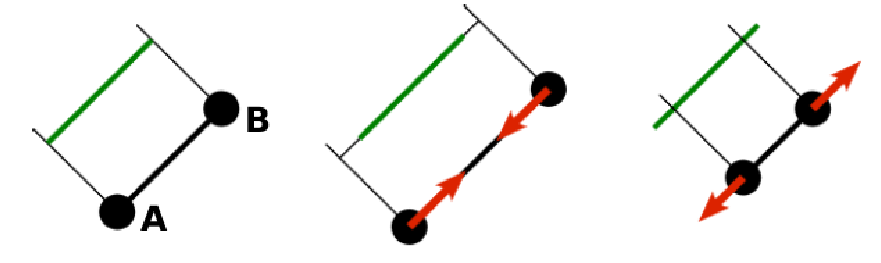
\includegraphics[width=8cm]{figures/stretching.png}
\end{center}
The stretching force acts between two particles and is symmetric. Therefore if an interaction is defined by
\begin{verbatim} 
inter 1 stretching_force 2.0 4.0
\end{verbatim}
then the following two commands
\begin{verbatim} 
part 42 bond 1 43
part 43 bond 1 42
\end{verbatim}
are equivalent.

\subsection{Linear stretching force}
\index{linear stretching force|mainindex}
\index{interactions!linear stretching force|mainindex}

\begin{essyntax}
  inter \var{bondid}
  stretchlin_force
  \var{L^0_{AB}} \var{k_slin}
\end{essyntax}
This type of interaction is available for closed 3D immersed objects as well as 
for 2D sheet flowing in the 3D flow. 

This type of interaction is the linear equivalent of stretching_force. The expressions for the forces are 
the same except $\kappa(\lambda_{AB}) = 1$. 


\subsection{Bending force}
\index{bending force|mainindex}
\index{interactions!bending force|mainindex}

\begin{essyntax}
  inter \var{bondid}
  bending_force
  \var{\theta^0} \var{k_b}
\end{essyntax}

The tendency of an elastic object to maintain the resting shape is governed by 
prescribing the prefered angles between the neighbouring triangles of the mesh. 
This type of interaction is available for closed 3D immersed objects as well as 
for 2D sheet flowing in the 3D flow.


Denote by $\theta^0$ the angle between two triangles in the resting shape. For 
closed immersed objects, you always have to set the inner angle. The deviation 
of this angle $\Delta \theta = \theta - \theta^0$ is computed and defines two 
bending forces for two triangles \var{A_1BC} and \var{A_2BC}
\begin{equation}
\var{F_{bi}(A_iBC)} = \var{k_b}\frac{\Delta \theta}{\theta^0} \var{n_{A_iBC}}
\end{equation}
Here, \var{n_{A_iBC}} is the unit normal vector to the triangle \var{A_iBC}. The 
force \var{F_{bi}(A_iBC)} is assigned to the vertex not belonging to the common 
edge. The opposite force divided by two is assigned to the two vertices lying on 
the common edge. This procedure is done twice, for $\var{i}=1$ and for 
$\var{i}=2$.

\begin{center}
  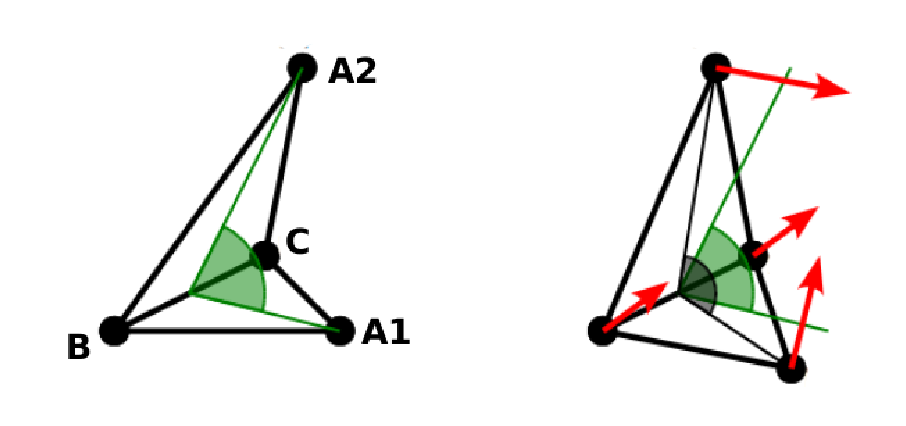
\includegraphics[width=8cm]{figures/bending.png}
\end{center}

Unlike the stretching force the bending force is strictly asymmetric. After 
creating an interaction
\begin{verbatim} 
inter 33 bending_force 0.7 4.0
\end{verbatim}
it is important how the bond is created. Particles need to be mentioned in the 
correct order. Command
\begin{verbatim} 
part 0 bond 33 1 2 3
\end{verbatim}
creates a bond related to the angle between the triangles 012 and 123. The particle 
0 corresponds to point A1, particle 1 to C, particle 2 to B and particle 3 to A2. 
There are two rules that need to be fulfilled:
\begin{itemize}
\item there has to be an edge between particles 1 and 2
\item orientation of the triangle 012, that is the normal vector 
defined as a vector product $01 \times 02$, must point to the inside of the immersed 
object.
\end{itemize}
Notice that also concave objects can be defined. If $\theta_0$ is larger than $\pi$, 
then the inner angle is concave.

\subsection{Local area conservation}
\index{local area conservation|mainindex}
\index{interactions!local area conservation|mainindex}

\begin{essyntax}
  inter \var{bondid}
  area_force_local
  \var{S^0_{ABC}} \var{k_{al}}
\end{essyntax}
This interaction conserves the area of the triangles in the triangulation. This 
type of interaction is available for closed 3D immersed objects as well as for 2D 
sheet flowing in the 3D flow.

The deviation of the triangle surface \var{S_{ABC}} is computed from the triangle 
surface in the resting shape $\Delta \var{S_{ABC}} = \var{S_{ABC}} - \var{S_{ABC}^0}$. 
The area constraint assigns the following  shrinking/expanding force to every vertex 
\begin{equation}
 \var{F_{al}(A)} = -\var{k_{al}}\frac{\Delta \var{S_{ABC}}}{\var{S_{ABC}}}\var{w_{A}}
\end{equation}
where \var{k_{al}}  is the area constraint coefficient, and \var{w_{A}} is the unit 
vector pointing from the centroid of triangle \var{ABC} to the vertex \var{A}. 
Similarly the analogical forces are assigned to \var{B} and \var{C}. This interaction 
is symmetric, therefore after defining the interaction
\begin{verbatim} 
inter 44 area_force_local 0.02 4.0
\end{verbatim}
the following commands are equivalent
\begin{verbatim} 
part 0 bond 44 1 2
part 0 bond 44 2 1
part 1 bond 44 0 2
\end{verbatim}

\subsection{Global area conservation}
\index{global area conservation|mainindex}
\index{interactions!global area conservation|mainindex}

\begin{essyntax}
  inter \var{bondid}
  area_force_global
  \var{S^0} \var{k_{ag}}
\end{essyntax}
This type of interaction is available solely for closed 3D immersed objects.

The conservation of local area is sometimes too restrictive. Denote by \var{S} the 
current surface of the immersed object, by \var{S_0} the surface in the relaxed 
state and define $\Delta \var{S} = \var{S} - \var{S_0}$. The global area conservation 
force is defined as
\begin{equation}
\var{F_{ag}(A)} = - \var{k_{ag}}\frac{\Delta \var{S}}{\var{S}}\var{w_{A}}
\end{equation}
Here, the above mentioned force divided by 3 is added to all three particles.
\begin{center}
  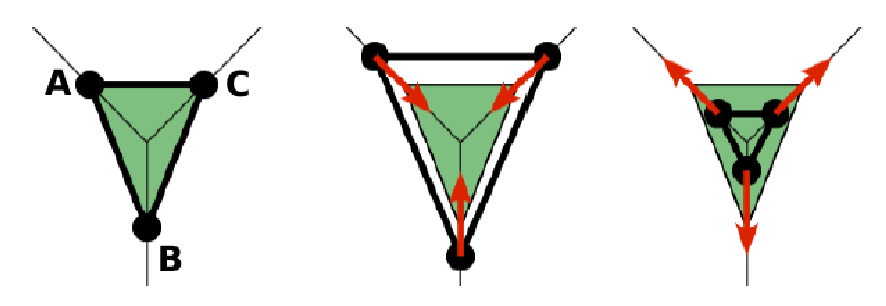
\includegraphics[width=8cm]{figures/arealocal.png}
\end{center}
Again, this interaction is symmetric, as is the area\_{}force\_{}local.

\subsection{Volume conservation}
\index{volume conservation|mainindex}
\index{interactions!volume conservation|mainindex}

\begin{essyntax}
  inter \var{bondid}
  volume_force
  \var{V^0} \var{k_v}
\end{essyntax}
This type of interaction is available solely for closed 3D immersed objects.

The deviation of the objects volume \var{V} is computed from the volume in 
the resting shape $\Delta \var{V} = \var{V} - \var{V^0}$. For each triangle the following 
force is computed
\begin{equation}
\var{F_v(ABC)} = -\var{k_v}\frac{\Delta \var{V}}{\var{V^0}} \var{S_{ABC}}\ \var{n_{ABC}}
\end{equation}
where \var{S_{ABC}} is the area of triangle \var{ABC}, \var{n_{ABC}} is the normal unit 
vector of plane \var{ABC}, and \var{k_v} is the volume constraint coefficient. The volume 
of one immersed object is computed from
\begin{equation}
\var{V} = \sum_{\var{ABC}}\var{S_{ABC}}\ \var{n_{ABC}}\cdot \var{h_{ABC}}
\end{equation}
where the sum is computed over all triangles of the mesh and \var{h_{ABC}} is the normal 
vector from the centroid of triangle \var{ABC} to any plane which does not cross the cell. 
The force \var{F_v(ABC)} is equally distributed to all three vertices $\var{A},\var{B},
\var{C}.$

\begin{center}
  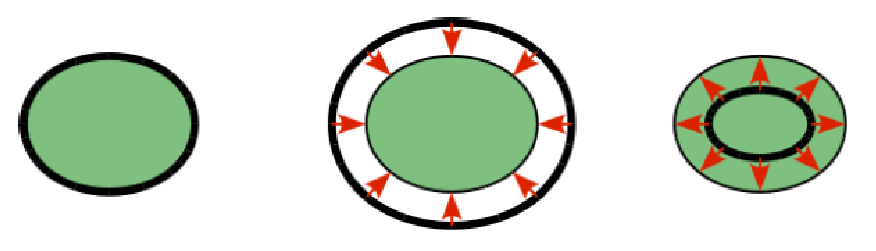
\includegraphics[width=8cm]{figures/volume.png}
\end{center}
This interaction is again symmetric. After the definition of the interaction by 
\begin{verbatim} 
inter 22 volume_force 65.3 3.0
\end{verbatim}
the order of vertices is crucial. By the following command the bonds are defined
\begin{verbatim} 
part 0 bond 22 1 2
\end{verbatim}
Triangle 012 must have correct orientation, that is the normal vector defined by a 
vector product $01\times02$. The orientation must point inside the immersed object.


\section{Bond-angle interactions}
\index{bond-angle interactions|mainindex}
\index{interactions!bond-angle|mainindex}
\label{sec:angle}

\begin{essyntax}
  \variant{1} inter \var{bondid} angle\_harmonic \var{K} \opt{\var{\phi_0}}
  \variant{2} inter \var{bondid} angle\_cosine \var{K} \opt{\var{\phi_0}}
  \variant{3} inter \var{bondid} angle\_cossquare \var{K} \opt{\var{\phi_0}}
  \begin{features}
    \required{BOND_ANGLE}
  \end{features}
\end{essyntax}

This creates a bond type with identificator \var{bondid}
with an angle dependent potential. This potential is defined between
three particles. The particle for which the bond is created, is the
central particle, and the angle $\phi$ between the vectors from this
particle to the two others determines the interaction.  \var{K} is the
bending constant, and the optional parameter $\var{\phi_0}$ is the
equilibirum bond angle in radian ranging from 0 to $\pi$.  If this
parameter is not given, it defaults to $\var{\phi_0} = \pi$, which
corresponds to a stretched configuration. For example, for a bond
defined by
\begin{code}
  part \$p_2 bond 4 \$p_1 \$p_3
\end{code}
the minimal energy configurations are the following:
\begin{center}
  \setlength{\unitlength}{3000sp}
  \begin{picture}(8381,2684)(1570,-5393)
    \thinlines
    \put(2701,-4561){\circle*{450}}
    \put(3601,-4561){\circle*{450}}
    \put(4501,-4561){\circle*{450}}
    \put(7021,-4561){\circle*{450}}
    \put(7921,-4561){\circle*{450}}
    \put(7921,-3661){\circle*{450}}
    \thicklines
    \put(2701,-4561){\line( 1, 0){1800}}
    \put(7021,-4561){\line( 1, 0){900}}
    \put(7921,-4561){\line( 0, 1){900}}
    \put(5761,-2831){\line( 0,-1){2500}}

    \put(2701,-5191){\makebox(0,0)[b]{$p_1$}}
    \put(3601,-5191){\makebox(0,0)[b]{$p_2$}}
    \put(4501,-5191){\makebox(0,0)[b]{$p_3$}}
    \put(7021,-5191){\makebox(0,0)[b]{$p_1$}}
    \put(8371,-3751){\makebox(0,0)[b]{$p_3$}}
    \put(7921,-5191){\makebox(0,0)[b]{$p_2$}}
    \put(8371,-2941){\makebox(0,0)[b]{\keyword{inter 4 angle\var{\_type} 1.0 [expr [PI]/2]}}}
    \put(3601,-2941){\makebox(0,0)[b]{\keyword{inter 4 angle\var{\_type} 1.0 [PI]}}}
  \end{picture}%
\end{center}

For the potential acting between the three particles three variants are possible
\begin{itemize}
\item Harmonic bond angle potential \variant{1}:\\
  A classical harmonic potential,
  \begin{equation}
    V(\phi) = \frac{K}{2} \left(\phi - \phi_0\right)^2.
  \end{equation}
  Unlike the two following variants, this potential has a kink at
  $\phi=\phi_0+\pi$ and accordingly a discontinuity in the force, and should
  therefore be used with caution.
\item Cosine bond angle potential \variant{2}:\\
  \begin{equation}
    V(\alpha) = K \left[1 - \cos(\phi - \phi0)\right]
  \end{equation}
  Around $\phi_0$, this potenial is close to a harmonic one (both are
  $1/2(\phi-\phi_0)^2$ in leading order), but it is periodic and smooth for all
  angles $\phi$.
\item Cosine square bond angle potential \variant{3}:\\
  \begin{equation}
    V(\alpha) = \frac{K}{2} \left[\cos(\phi) - \cos(\phi_0)\right]^2
  \end{equation}
  This form is used for example in the GROMOS96 force field. The potential is
  $1/8(\phi-\phi_0)^4$ around $\phi_0$, and therefore much flatter than the
  two potentials before.
\end{itemize}

\section{Dihedral interactions}
\index{dihedral interactions|mainindex}
\index{interactions!dihedral|mainindex}
\label{sec:dihedral}

\begin{essyntax}
  inter \var{bondid} dihedral \var{n} \var{K} \var{p}
\end{essyntax}

This creates a bond type with identificator \var{bondid}
with a dihedral potential, \ie a four-body-potential. In the following,
let the particle for which the bond is created be particle $p_2$, and
the other bond partners $p_1$, $p_3$, $p_4$, in this order, \ie
\lit{part $p_2$ bond bondid $p_1$ $p_3$ $p_4$}. Then, the
dihedral potential is given by
\begin{equation}
  V(\phi) = \var{K}\left[1 - \cos(\var{n}\phi - \var{p})\right],
\end{equation}
where \var{n} is the multiplicity of the potential (number of minimas)
and can take any integer value (typically from 1 to 6), $p$ is a phase
parameter and \var{K} is the bending constant of the potential. $\phi$
is the dihedral angle between the particles defined by the particle
quadrupel $p_1$, $p_2$, $p_3$ and $p_4$, \ie the angle between the
planes defined by the particle triples $p_1$, $p_2$ and $p_3$ and
$p_2$, $p_3$ and $p_4$:
\begin{center}
  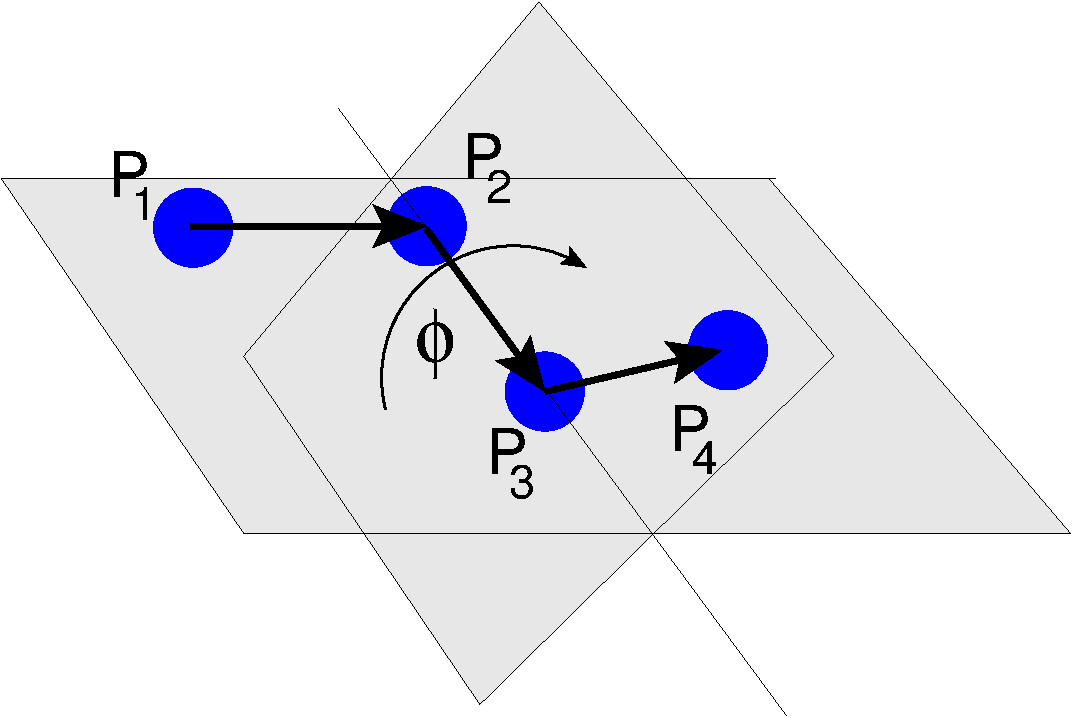
\includegraphics[height=8em]{figures/dihedral-angle}
\end{center}
Together with appropriate Lennard-Jones interactions, this potential
can mimic a large number of atomic torsion potentials.

If you enable the feature OLD_DIHEDRAL, then the old, less
general form of the potential is used:
\begin{equation}
  V(\phi) = \var{K}\left[1 + \var{p}\,\cos(\var{n}\phi)\right],
\end{equation}
where $p$ is rather a phase factor and can only take values $p=\pm 1$.


\section{Coulomb interaction}
\label{sec:inter-electrostatics}
\index{Coulomb interactions|mainindex}
\index{Electrostatic interactions|mainindex}
\index{interactions!Coulomb|mainindex}
\index{interactions!Electrostatic|mainindex}

\begin{essyntax}
  \variant{1} inter coulomb 0.0
  \variant{2} inter coulomb
  \variant{3} inter coulomb \var{parameters}
\end{essyntax}

These commands allow to set up the calculation of the Coulomb
interaction.  The Coulomb (or electrostatic) interaction is defined as
follows.  For a pair of particles at distance $r$ with charges $q_1$
and $q_2$, the interaction is given by
\begin{equation}
  U^C(r)=l_B k_B T\frac{q_1 q_2}{r}.
\end{equation}
where $l_B = e_o^2 / (4 \pi \epsilon k_B T)$ denotes the Bjerrum
length, which measures the strength of the electrostatic interaction.
As a special case, when the internal variable \var{temperature} 
is set to zero, the value of bjerrum length you enter 
is treated as $l_B k_B T$ rather than $l_B$. This occurs when the
thermostat is switched off and \es performs an NVE integration
(see also Section~\ref{sec:thermostat}).

Computing electrostatic interactions is computationally very
expensive.  \es{} features some state-of-the-art algorithms to deal
with these interactions as efficiently as possible, but almost all of
them require some knowledge to use them properly.  Uneducated use can
result in completely unphysical simulations.

Variant \variant{1} disables Coulomb interactions.  Variant
\variant{2} returns the current parameters of the coulomb interaction
as a Tcl-list using the same syntax as used to setup the method, \eg
\begin{tclcode}
  {coulomb 1.0 p3m 7.75 8 5 0.1138 0.0}
  {coulomb epsilon 0.1 n_interpol 32768 mesh_off 0.5 0.5 0.5}
\end{tclcode}

Variant \variant{3} is the generic syntax to set up a specific method
or its parameters, the details of which are described in the following
subsections.  Note that using the electrostatic interaction also
requires assigning charges to the particles.  This is done using the
\texttt{part} command to set the charge \texttt{q}, \eg
\begin{tclcode}
  inter coulomb 1.0 p3m tune accuracy 1e-4
  part 0 q 1.0; part 1 q -1.0
\end{tclcode}

\subsection{Coulomb P3M}
\label{sec:coulomb}
\index{P3M method|mainindex}
\index{interactions!P3M|mainindex}

\begin{essyntax}
  inter coulomb \var{l_B} p3m [gpu] 
  \var{r_\mathrm{cut}} \alt{\var{mesh} \asep \{\var{mesh_x} \var{mesh_y} \var{mesh_z}\}} \var{cao} \var{alpha}
  \begin{features}
    \required{ELECTROSTATICS}
  \end{features}
\end{essyntax}

For this feature to work, you need to have the \texttt{fftw3} library
installed on your system. In \es{}, you can check if it is compiled in
by checking for the feature \texttt{FFTW}.

This command activates the P3M method to compute the electrostatic
interactions between charged particles.  The different parameters are
described in more detail in \cite{deserno98a}.
\begin{description}
\item[\var{[gpu]}]
The optional flag gpu causes the far field portion of p3m to be calculated on the GPU.  It should be noted that this does not always provide significant increase in performance.  Furthermore it computes the far field interactions with only single precision which limits the maximum precision.  Furthermore the algorithm does not work in combination with certain other methods implemented in ESPResSo and only for the case of cubic boxes.
\item[\var{r_\mathrm{cut}}] The real space cutoff as a positive
  floating point number.
\item[\var{mesh}] The number of mesh points, as a single positive
  integer.
\item[\var{mesh_{x,y,z}}] The number of mesh points in x, y and z
  direction. This is relevant for noncubic boxes.
\item[\var{cao}] The \emph{charge-assignment order}, an integer
  between $0$ and $7$.
\item[\var{alpha}] The Ewald parameter as a positive floating point
  number.
\end{description}

Make sure that you know the relevance of the P3M parameters before
using P3M! If you are not sure, read the following references
\cite{ewald21, hockney88, kolafa92, deserno98, deserno98a, deserno00,
  deserno00a, cerda08a}.


\subsubsection{Tuning Coulomb P3M}
\label{ssec:tunep3m}
\begin{essyntax}
  inter coulomb \var{l_B} p3m \alt{tune \asep tunev2} [gpu]
  accuracy \var{accuracy}\\
  \opt{r_cut \var{r_\mathrm{cut}}}
  \opt{mesh \var{mesh}}
  \opt{cao \var{cao}}
  \opt{alpha \var{\alpha}}
  \begin{features}
    \required{ELECTROSTATICS}
  \end{features}
\end{essyntax}

It is not easy to calculate the various parameters of the P3M method
such that the method provides the desired accuracy at maximum speed.
To simplify this, \es{} provides a function to automatically tune the
algorithm.  Note that for this function to work properly, your system
should already contain an initial configuration of charges and the
correct initial box size. Also note that both provided tuning
algorithms work very well on homogenous charge distributions, but
might not achieve the requested precision for highly inhomogenous or
symmetric systems. For example, because of the nature of the P3M
algorithm, systems are problematic where most charges are placed in
one plane, one small region, or on a regular grid.

The function employs the analytical expression of the error estimate
for the P3M method \cite{hockney88} and its real space error
\cite{kolafa92} to obtain sets of parameters that yield the desired
accuracy, then it measures how long it takes to compute the coulomb
interaction using these parameter sets and chooses the set with the
shortest run time.

The function will only automatically tune those parameters that are
not set to a predetermined value using the optional parameters of the
tuning command.

The two tuning methods follow different methods for determining the
optimal parameters. While the \keyword{tune} version tests different
values on a grid in the parameter space, the \keyword{tunev2} version
uses a bisection to determine the optimal parameters.  In general, for
small systems the \keyword{tune} version is faster, while for large
systems \keyword{tunev2} is faster. The results of \keyword{tunev2}
are always at least as good as the parameters from the \keyword{tune}
version, and normally the obtained accuracy is much closer to the
desired value.

During execution the tuning routines report the tested parameter sets,
the corresponding k-space and real-space errors and the timings needed
for force calculations (the setmd variable \var{timings} controls the
number of test force calculations).  Since the error depends on
\var{r_\mathrm{cut}}/\var{box\_l} and \var{\alpha}\var{box\_l} the
output is given in these units.

Note that the previous setting of \var{r_\mathrm{cut}}, \var{cao} and
\var{mesh} will be remembered.  If you want to retune your
electrostatics, \eg after a major system change, you should use
\begin{code}
  inter coulomb \var{l_B} p3m tune accuracy \var{acc} r_cut 0 mesh 0 cao 0
\end{code}

\subsubsection{Additional P3M parameters}

\begin{essyntax}
  inter coulomb \opt{\lit{epsilon} \alt{\lit{metallic} \asep \var{epsilon}}}
  \opt{\lit{n_interpol} \var{points}} \opt{\lit{mesh_off} \var{xoff}
    \var{yoff} \var{zoff}}
\end{essyntax}

Once P3M algorithm has been set up, it is possible to set some
additional P3M parameters with this command.  The different parameters
have the following meaning:
\begin{description}
\item[\lit{epsilon} \var{epsilon}] The dielectric constant of the
  surrounding medium, metallic (\ie infinity) or some finite positive
  number.  Defaults to \lit{metallic}.
\item[\lit{n_interpol} \var{n_interpol}] Number of interpolation
  points for the charge assignment function.  When this is set to $0$,
  interpolation is turned off and the function is computed directly.
  Defaults to $32768$.
\item[\lit{mesh_off} \var{mesh_off}] Offset of the first mesh point
  from the lower left corner of the simulation box in units of the
  mesh constant. Defaults to \codebox{{0.5 0.5 0.5}}.
\end{description}


\subsection{Debye-H\"uckel potential}
\index{Debye-H\"uckel potential|mainindex}
\index{interactions!Debye-H\"uckel|mainindex}

\begin{essyntax}
  inter coulomb \var{l_B} dh \var{\kappa} \var{r_\mathrm{cut}}
  \begin{features}
    \required{ELECTROSTATICS}
  \end{features}
\end{essyntax}

Defines the electrostatic potential by
\begin{equation}
  U^{C-DH} = l_B k_B T \frac{q_1 q_2 exp(-\kappa r)}{r}\quad \mathrm{for}\quad r<r_{\mathrm{cut}}
\end{equation}

The Debye-H\"uckel potential is an approximate method for calculating
electrostatic interactions, but technically it is treated as other
short-ranged non-bonding potentials. For $r>r_{\mathrm cut}$ it is set 
to zero which introduces a step in energy. Therefore, it introduces
fluctuations in energy.

For $\kappa = 0$, this corresponds to the plain coulomb potential.

\subsection{MMM2D}
\index{MMM2D method|mainindex}
\index{interactions!MMM2D|mainindex}

\begin{citebox}
  Please cite~\citewbibkey{mmm2d} when using MMM2D, and
  \citewbibkey{icmmm2d} when using dielectric interfaces.
\end{citebox}


\begin{essyntax}
 inter coulomb \var{l_B} mmm2d \var{maximal\_pairwise\_error}
 \opt{\var{fixed\_far\_cutoff}}
 \opt{dielectric \var{\epsilon_t} \var{\epsilon_m} \var{\epsilon_b}}
 \opt{dielectric-contrasts \var{\Delta_t} \var{\Delta_b}}
 \opt{capacitor \var{U}}
  \begin{features}
    \required{ELECTROSTATICS}
  \end{features}
\end{essyntax}
MMM2D coulomb method for systems with periodicity 1 1 0. Needs the
layered cell system. The performance of the method depends on the
number of slices of the cell system, which has to be tuned manually.
It is automatically ensured that the maximal pairwise error is smaller
than the given bound. The far cutoff setting should only be used for
testing reasons, otherwise you are more safe with the automatical
tuning. If you even don't know what it is, do not even think of
touching the far cutoff. For details on the MMM family of algorithms,
refer to appendix \vref{chap:mmm}.

The last two, mutually exclusive arguments ``dielectric'' and
``dielectric-constants'' allow to specify dielectric contrasts at the
upper and lower boundaries of the simulation box. The first form
specifies the respective dielectric constants in the media, which
however is only used to calculate the contrasts. That is, specifying 
$\epsilon_t=\epsilon_m=\epsilon_b=\text{const}$ is always identical to
$\epsilon_t=\epsilon_m=\epsilon_b=1$. The second form specifies only
the dielectric contrasts at the boundaries, that is
$\Delta_t=\frac{\epsilon_m-\epsilon_t}{\epsilon_m+\epsilon_t}$ and
$\Delta_b=\frac{\epsilon_m-\epsilon_b}{\epsilon_m+\epsilon_b}$. Using
this form allows to choose $\Delta_{t/b}=-1$, corresponding to
metallic boundary conditions.

Using \keyword{capacitor} \var{U} allows to maintain a constant 
electric potential difference \var{U} between the xy-plane at $z=0$ 
and $z=L$, where $L$ denotes the box length in $z$-direction.
This is done by countering the total dipol moment of
the system with the electric field $E_{induced}$ and superposing 
a homogeneous electric field $E_{applied} = \frac{U}{L}$ 
to retain \var{U}. This mimics the induction of surface charges
$\pm\sigma = E_{induced} \cdot \epsilon_0$ for planar electrodes at $z=0$ 
and $z=L$ in a capacitor connected to a battery with voltage \var{U}.
Using \var{capacitor} 0 is equivalent to $\Delta_{t/b}=-1$.

\begin{essyntax}
  efield_caps \alt{total \asep induced \asep applied}
  \begin{features}
    \required{ELECTROSTATICS}
  \end{features}
\end{essyntax}

The electric fields added by \var{capacitor} \var{U} can be obtained 
by calling the above command, where \var{induced} returns $E_{induced}$,
\var{applied} returns $E_{applied}$ and \var{total} their sum.

\subsection{MMM1D}
\index{MMM1D method|mainindex}
\index{interactions!MMM1D|mainindex}

\begin{citebox}
  Please cite~\citewbibkey{mmm1d} when using MMM1D.
\end{citebox}

\begin{essyntax}
  \variant{1}
  inter coulomb \var{l_B} mmm1d \var{switch\_radius}
  \var{maximal\_pairwise\_error}

  \variant{2}
  inter coulomb \var{l_B} mmm1d tune \var{maximal\_pairwise\_error}
  \begin{features}
    \required{ELECTROSTATICS}
  \end{features}
\end{essyntax}
MMM1D coulomb method for systems with periodicity 0 0 1. Needs the
nsquared cell system (see section \vref{sec:cell-systems}). The first
form sets parameters manually. The switch radius determines at which
xy-distance the force calculation switches from the near to the far
formula. The Bessel cutoff does not need to be specified as it is
automatically determined from the particle distances and maximal
pairwise error. The second tuning form just takes the
maximal pairwise error and tries out a lot of switching radii to find
out the fastest one. If this takes too long, you can change the value
of the setmd variable \keyword{timings}, which controls the number of
test force calculations.

\begin{essyntax}
  \variant{1}
  inter coulomb \var{l_B} mmm1dgpu \var{switch\_radius}
  \opt{\var{bessel\_cutoff}} \var{maximal\_pairwise\_error}

  \variant{2}
  inter coulomb \var{l_B} mmm1dgpu tune \var{maximal\_pairwise\_error}
  \begin{features}
    \required{CUDA}
	\required{ELECTROSTATICS}
	\required{MMM1D_GPU}
  \end{features}
\end{essyntax}
MMM1D is also available in a GPU implementation. Unlike its CPU
counterpart, it  does not need the nsquared cell system. The first
form sets parameters manually. The switch radius determines at which
xy-distance the force calculation switches from the near to the far
formula. If the Bessel cutoff is not explicitly given, it is
determined from the maximal pairwise error, otherwise this error only
counts for the near formula. The second tuning form just takes the
maximal pairwise error and tries out a lot of switching radii to find
out the fastest one.

For details on the MMM family of algorithms, refer to appendix
\vref{chap:mmm}.

\subsection{Maxwell Equation Molecular Dynamics (MEMD)}
\index{Maggs method|mainindex}
\index{Maxwell Equation Molecular Dynamics|mainindex}
\index{MEMD|mainindex}
\index{interactions!Maggs method|mainindex}
\index{interactions!MEMD|mainindex}

\begin{essyntax}
  inter coulomb \var{l_B}
  memd \var{f\_mass} \var{mesh} \opt{epsilon \var{\varepsilon_{\infty}}}
  \begin{features}
    \required{ELECTROSTATICS}
  \end{features}
\end{essyntax}

This is an implementation of the instantaneous 1/r Coulomb interaction
\begin{equation}
  U = l_B k_B T \frac{q_1 q_2}{r}
\end{equation}
as the potential of mean force between charges which are dynamically
coupled to a local electromagnetic field.

The algorithm currently works with the following constraints:

\begin{itemize}
  \item cellsystem has to be domain decomposition but \emph{without}
    Verlet lists!
  \item system has to be periodic in three dimensions.
\end{itemize}

\begin{arguments}
\item[\var{f\_mass}] is the mass of the field degree of freedom and equals
  to the square root of the inverted speed of light.
\item[\var{mesh}] is the number of mesh points for the interpolation
  of the electromagnetic field in one dimension.
\item[\var{\varepsilon_{\infty}}] is the background dielectric
  permittivity at infinity. This defaults to metallic boundary
  conditions, to match the results of P3M.
\end{arguments}

The arising self-interactions are treated with a modified version of
the exact solution of the lattice Green's function for the
problem.

Currently, forces have large errors for two particles within the same
lattice cube. This may be fixed in future development, but right now
leads to the following rule of thumb for the parameter choices:

\begin{itemize}
  \item The lattice should be of the size of your particle size
    (i.e. the lennard jones epsilon). That means: $\text{mesh} \approx
    \text{box\_l} / \text{lj\_sigma}$
  \item The integration timestep should be in a range where no
    particle moves more than one lattice box (i.e. lennard jones
    sigma) per timestep.
  \item The speed of light should satisfy the stability criterion
    $c\ll a/dt$, where $a$ is the lattice spacing and $dt$ is the
    timestep. For the second parameter, this means $\text{f\_mass} \gg
    dt^2/a^2$.
\end{itemize}

The main error of the MEMD algorithm stems from the lattice
interpolation and is proportional to the lattice size in three
dimensions, which means $\Delta_\text{lattice} \propto a^3$.

Without derivation here, the algorithmis error is proportional to
$1/c^2$, where $c$ is the adjustable speed of light. From the
stability criterion, this yields

\begin{equation}
\Delta_\text{maggs} = A\cdot a^3 + B\cdot dt^2/a^2
%\label{eq:maggserror}
\end{equation}

This means that increasing the lattice will help the algorithmic
error, as we can tune the speed of light to a higher value. At the
same time, it increases the interpolation error at an even higher
rate. Therefore, momentarily it is advisable to choose the lattice
with a rather fine mesh of the size of the particles. As a rule of
thumb, the error will then be less than $10^{-5}$ for the particle
force.

For a more detailed description of the algorithm, see
appendix~\vref{sec:MEMD} or the publications~\cite{maggs02a,
  pasichnyk04a}.

\subsubsection{Spatially varying dielectrics with MEMD}
\index{Dielectric interfaces}
\label{sec:dielectric-memd}

Since MEMD is a purely local algorithm, one can apply local changes
to some properties and the propagation of the Coulomb force is still
valid. In particular, it is possible to arbitrarily select the
dielectric permittivity on each site of the interpolating lattice.

\begin{essyntax}
  inter coulomb \var{l_B}
  memd localeps node \var{node\_x} \var{node\_y} \var{node\_z}
  dir \var{X/Y/Z} eps \var{\varepsilon}
  \begin{features}
    \required{ELECTROSTATICS}
  \end{features}
\end{essyntax}

The keyword \keyword{localeps} after the \keyword{inter coulomb}
command offers the possibility to assign any value of $\varepsilon$
to any lattice site.

\begin{arguments}
\item[\var{l_B}] is the bjerrum length of the background. It defines
	the reference value $\varepsilon_\text{bg}$ via the formula 
	\eqref{eq:bjerrum-length}. This is a global variable.
\item[\var{node\_x}] is the index of the node in $x$ direction that
	should be changed
\item[\var{node\_y}] is the index of the node in $y$ direction that
	should be changed
\item[\var{node\_z}] is the index of the node in $z$ direction that
	should be changed
\item[\var{X/Y/Z}] is the direction in which the lattice site to be
	changed is pointing. Has to be one of the three (X, Y or Z).
\item[\var{\varepsilon}] is the relative permittivity change in
	respect to the background permittivity set by the parameter
	\var{l_B}.
\end{arguments}

The permittivity on each lattice site is set relatively. By defining
the (global) bjerrum length of the system, the reference
permittivity~$\varepsilon$ is fixed via the formula

\begin{equation}
l_B = e^2 / (4 \pi \varepsilon k_B T)
\label{eq:bjerrum-length}
\end{equation}

The local changes of $\varepsilon$ are in reference to this value
and can be seen as a spatially dependent prefactor to this epsilon.
If left unchanged, this prefactor is $1.0$ for every site by
default.

\subsection{Electrostatic Layer Correction (ELC)}
\index{ELC method|mainindex}
\index{interactions!ELC method|mainindex}

\begin{citebox}
  Please cite~\citewbibkey{elc} when using ELC, and in addition
  \citewbibkey{icelc} if you use dielectric interfaces.
\end{citebox}

\begin{essyntax}
  inter coulomb elc \var{maximal\_pairwise\_error} \var{gap\_size}
  \opt{\var{far\_cutoff}}
  \opt{noneutralization}
  \opt{dielectric \var{\epsilon_t} \var{\epsilon_m} \var{\epsilon_b}}
  \opt{dielectric-contrasts \var{\Delta_t} \var{\Delta_b}}
  \opt{capacitor \var{U}}
  \begin{features}
    \required{ELECTROSTATICS}
  \end{features}
\end{essyntax}
This is a special procedure that converts a 3d method, to a 2d method,
in computational order N. Currently, it only supports P3M. This means,
that you will first have to set up the P3M algorithm (via
\texttt{inter coulomb p3m \var{params}}) before using ELC.  The
algorithm is definitely faster than MMM2D for larger numbers of
particles ($>400$ at reasonable accuracy requirements). The maximal
pairwise error \var{maximal\_pairwise\_error} sets the LUB error of
the force between any two charges without prefactors (see the
papers). The algorithm tries to find parameters to meet this LUB
requirements or will throw an error if there are none.

The gap size \var{gap\_size} gives the height of the empty region
between the system box and the neighboring artificial images (again,
see the paper).  \es does not make sure that the gap is actually
empty, this is the users responsibility. The method will compute fine
of the condition is not fulfilled, however, the error bound will not
be reached. Therefore you should really make sure that the gap region
is empty (e. g. by constraints).

The setting of the far cutoff \var{far\_cutoff} is only intended for
testing and allows to directly set the cutoff. In this case, the
maximal pairwise error is ignored. The periodicity has to be set to
\texttt{1 1 1} still, and the 3d method has to be set to epsilon
metallic, i.e.  metallic boundary conditions. For details, see
appendix \vref{chap:mmm}.

By default, ELC just as P3M adds a homogeneous neutralizing background
to the system in case of a net charge. However, unlike in three
dimensions, this background adds a parabolic potential across the
slab~\cite{ballenegger09a}. Therefore, under normal circumstance, you
will probably want to disable the neutralization using
\opt{noneutralization}. This corresponds then to a formal
regularization of the forces and energies~\cite{ballenegger09a}. Also,
if you add neutralizing walls explicitely as constraints, you have to
disable the neutralization.

The dielectric contrast features work exactly the same as for MMM2D,
see the documentation above. Same accounts for \keyword{capacitor} 
\var{U}, but the constant potential is maintained between the xy-plane
at $z=0$ and $z=L-gap\_size$. The command \var{efield\_caps} to read  
out the electric fields added by \var{capacitor} \var{U} also applies 
for the capacitor-feature of ELC.

Make sure that you read the papers on ELC (\cite{elc,icelc})
before using it.

\subsection{Dielectric interfaces with the ICC$\star$ algorithm}
\index{ICC$\star$|mainindex}
\index{Dielectric interfaces}
\newescommand{iccp3m}

\begin{essyntax}
  iccp3m \var{n\_induced\_charges} 
  convergence \var{convergence\_criterion}
  areas \var{areas}
  normals \var{normals}
  sigmas \var{sigmas}
  epsilons \var{epsilons}
  \opt{eps\_out \var{eps\_out} }
  \opt{relax \var{relaxation\_parameter} }
  \opt{max\_iterations \var{max\_iterations} }
  \opt{ext\_field \var{ext\_field}}
  \begin{features}
    \required{ELECTROSTATICS}
  \end{features}
\end{essyntax}

The ICC$\star$ algorithm allows to take into account arbitrarily
shaped dielectric interfaces.  This is done by iterating the charge on
the particles with the ids 0 to \var{n\_induced\_particles-1} until
the correctly represent the influence of the dielectric
discontinuity. It relies on a coulomb solver that is already
initialized. This Coulomb solver can be P3M, P3M+ELC, MMM2D or MMM1D.
As most of the times, ICC$\star$ will be used with P3M the
corresponding command is called \keyword{iccp3m}.

Please make sure to read the corresponding articles,
mainly\cite{espresso2, tyagi10a, kesselheim11a} before using it.

The particles with ids 0 to \var{n\_induced\_particles-1} are treated
as iterated particles by ICC$\star$.  The constitute the dielectric
interface and should be fixed in space. The parameters \var{areas} and
\var{epsilons} are Tcl lists containing one floating point number
describing each surface elements area and dielectric
constant. \var{sigmas} allows to take into account a (bare) charge
density, thus a surface charge density in absence of any charge
induction. \var{normals} is a Tcl list of Tcl lists with three
floating point numbers describing the outward pointing normal vectors
for every surface element.  The parameter \var{convergence\_criterion}
allows to specify the accuracy of the iteration. It corresponds to the
maximum relative change of any of the interface particle's
charge. After \var{max\_iterations} the iteration stops anyways. The
dielectric constant in bulk, i.~e. outside the dielectric walls is
specified by \var{eps\_out}. A homogenous electric field can be added
to the calculation of dielectric boundary forces by specifying it in
the parameter \var{ext\_field}.

\subsubsection{Quick setup of dielectric interfaces}
\index{Dielectric interfaces}
\newescommand{dielectric}

\begin{essyntax}
  \variant{1} dielectric sphere center \var{cx} \var{cy} \var{cz} radius \var{r} res \var{res} 
  \variant{2} dielectric wall normal \var{nx} \var{ny} \var{nz} dist \var{d} res \var{res}
  \variant{3} dielectric cylinder  center \var{cx} \var{cy} \var{cz} axis \var{ax} \var{ay} \var{az} radius \var{r} direction \var{d} 
  \variant{4} dielectric pore center \var{cx} \var{cy} \var{cz}  axis \var{ax} \var{ay} \var{az} radius \var{r} length \var {l} smoothing\_radius \var{rs} res \var{res}
  \variant{5} dielectric slitpore pore_mouth \var{z} \
             channel_width \var{c} \
             pore_width \var{w} \
             pore_length \var{l} \
             upper_smoothing_radius \var{us} \
             lower_smoothing_radius \var{ls} 

\end{essyntax}

The command \keyword{dielectric} allows to conveniently create
dielectric interfaces similar to the constraint and the lbboundary
command. Currently the creation of spherical, cylindrical and planar
geometries as well as a pore and slitpore geometry is supported.
Please check the documentation of the corresponding constraint for the detailed geometry.
It is implemented
in Tcl and places particles in the right positions and adds the
correct values to the global Tcl variables \var{icc\_areas}
\var{icc\_normals} \var{icc\_sigmas} \var{icc\_epsilons} and increases
the global Tcl variable var{n\_induced\_charges}. Thus after setting
up the shapes, it is still necessary to register them by calling
\keyword{iccp3m}, usually in the following way:
\begin{code}
  iccp3m \$n\_induced\_charges epsilons \$icc\_epsilons normals \\ 
  \$icc\_normals areas \$icc\_areas sigmas \$icc\_sigmas
\end{code}

\section{Dipolar interaction}
\label{sec:inter-dipolar}
\index{Dipolar interactions|mainindex}
\index{Magnetostatic interactions|mainindex}
\index{interactions!Dipolar|mainindex}
\index{interactions!Magnetostatic|mainindex}

\begin{essyntax}
  \variant{1} inter magnetic 0.0
  \variant{2} inter magnetic
  \variant{3} inter magnetic \var{parameters}
\end{essyntax}

These commands can be used to set up magnetostatic interactions, which
is defined as follows:
\begin{equation}
  U^{D-P3M}(\vec{r}) = l_{B} k_B T \left( \frac{(\vec{\mu}_i \cdot \vec{\mu}_j)}{r^3} 
  - \frac{3  (\vec{\mu}_i \cdot \vec{r})  (\vec{\mu}_j \cdot \vec{r}) }{r^5} \right)
\end{equation}
where $r=|\vec{r}|$.

$l_{B}$ is a dimensionless parameter similar to the Bjerrum length in
electrostatics which helps to tune the effect of the medium on the
magnetic interaction between two magnetic dipoles.

Computing magnetostatic interactions is computationally very
expensive.  \es{} features some state-of-the-art algorithms to deal
with these interactions as efficiently as possible, but almost all of
them require some knowledge to use them properly.  Uneducated use can
result in completely unphysical simulations.

The commands above work as their couterparts for the electrostatic
interactions (see section \vref{sec:coulomb}).  Variant \variant{1}
disables dipolar interactions.  Variant \variant{2} returns the
current parameters of the dipolar interaction as a Tcl-list using the
same syntax as used to setup the method, \eg
\begin{tclcode}
  {coulomb 1.0 p3m 7.75 8 5 0.1138 0.0}
  {coulomb epsilon 0.1 n_interpol 32768 mesh_off 0.5 0.5 0.5}
\end{tclcode}

Variant \variant{3} is the generic syntax to set up a specific method
or its parameters, the details of which are described in the following
subsections.  Note that using the magnetostatic interaction also
requires assigning dipole moments to the particles.  This is done
using the \texttt{part} command to set the dipole moment \texttt{dip},
\eg
\begin{tclcode}
  inter coulomb 1.0 p3m tune accuracy 1e-4
  part 0 dip 1 0 0; part 1 dip 0 0 1
\end{tclcode}

\subsection{Dipolar P3M}

\begin{essyntax}
  inter magnetic \var{l_B} p3m 
  \var{r_\mathrm{cut}} \var{mesh} \var{cao} \var{alpha}
  \begin{features}
    \required{DIPOLES}
  \end{features}
\end{essyntax}

This command activates the P3M method to compute the dipolar
interactions between charged particles.  The different parameters are
described in more detail in \cite{cerda08a}.
\begin{description}
\item[\var{r_\mathrm{cut}}] The real space cutoff as a positive
  floating point number.
\item[\var{mesh}] The number of mesh points, as a single positive
  integer.
\item[\var{cao}] The \emph{charge-assignment order}, an integer
  between $0$ and $7$.
\item[\var{alpha}] The Ewald parameter as a positive floating point
  number.
\end{description}

Make sure that you know the relevance of the P3M parameters before
using P3M! If you are not sure, read the following references
\cite{ewald21, hockney88, kolafa92, deserno98, deserno98a, deserno00,
  deserno00a}.

Note that dipolar P3M does not work with non-cubic boxes.

\subsubsection{Tuning dipolar P3M}
\begin{essyntax}
  inter magnetic \var{l_B} p3m \alt{tune \asep tunev2}
  accuracy \var{accuracy}\\
  \opt{r_cut \var{r_\mathrm{cut}}} \opt{mesh \var{mesh}} \opt{cao
    \var{cao}} \opt{alpha \var{\alpha}}
  \begin{features}
    \required{DIPOLES}
  \end{features}
\end{essyntax}

Tuning dipolar P3M works exactly as tuning Coulomb P3M.  Therefore,
for details on how to tune the algorothm, refer to the documentation
of Coulomb P3M (see section \vref{ssec:tunep3m}).

For the magnetic case, the expressions of the error estimate are given
in \cite{cerda08a}.

\subsection{Dipolar Layer Correction (DLC)}
\index{DLC method|mainindex}
\index{interactions!DLC method|mainindex}

\begin{essyntax}
  inter magnetic mdlc \var{accuracy} \var{gap\_size}
  \opt{\var{far\_cutoff}}
  \begin{features}
    \required{DIPOLES}
  \end{features}
\end{essyntax}

Like ELC but applied to the case of magnetic dipoles, but here the
accuracy is the one you wish for computing the energy.
\var{far_cutoff} is set to a value that, assuming all dipoles to be as
larger as the largest of the dipoles in the system, the error for the
energy would be smaller thant the value given by accuracy. At this
moment you cannot compute the accuracy for the forces, or torques,
nonetheless, usually you will have an error for forces and torques
smaller than for energies. Thus, the error for the energies is an
upper boundary to all errors in the calculations.

At present, the program assumes that the gap without particles is
along the z-direction.  The gap-size is the length along the
z-direction of the volume where particles are not allowed to enter.

As a reference for the DLC method, see \cite{brodka04a}.

\subsection{Dipolar all-with-all and no replicas (DAWAANR)}
\index{DAWAANR method|mainindex}
\index{interactions!DAWAANR method|mainindex}

\begin{essyntax}
  inter magnetic \var{l_{B}} dawaanr
  \begin{features}
    \required{DIPOLES}
  \end{features}
\end{essyntax}

This interaction calculates energies and forces between dipoles by
explicitly summing over all pairs.  For the directions in which the
system is periodic (as defined by \texttt{setmd periodic}), it applies
the minimum image convention, i.e. the interaction is effectively cut
off at half a box length.

In periodic systems, this method should only be used if it is not possible to use dipolar P3M or
DLC, because those methods have a far better accuracy and are much faster.
In a non-periodic system, the DAWAANR-method gives the exact result.

\subsection{Magnetic Dipolar Direct Sum (MDDS)}
\index{MDDS method|mainindex}
\index{interactions!MDDS method|mainindex}

\begin{essyntax}
  inter magnetic \var{l_{B}} mdds n\_cut \var{value\_n\_cut}
  \begin{features}
    \required{DIPOLES}
    \required{MAGNETIC_DIPOLAR_DIRECT_SUM}
  \end{features}
\end{essyntax}

The command enables the ``magnetic dipolar direct sum''.  The
dipole-dipole interaction is computed by explicitly summing over all
pairs. If the system is periodic in one or more directions, the
interactions with further \var{value\_n\_cut} replicas of the system
in all periodic directions is explicitly computed.

As it is very slow, this method is not intended to do simulations,
but rather to check the results you get from more efficient methods
like P3M.
  
\section{Special interaction commands}
\label{sec:inter-other}

\subsection{Tunable-slip boundary interaction}\label{sec:tunableSlip}
\index{Tunable-slip boundary interaction|mainindex}
\index{interactions!Tunable-slip boundary interactions|mainindex}
\begin{essyntax}
  inter \var{type1} \var{type2}
  tunable_slip \var{T} \var{\gamma_L} \var{r_\mathrm{cut}} \var{\delta t}
  \var{v_x} \var{v_y} \var{v_z}
  \begin{features}
    \required{TUNABLE_SLIP}
  \end{features}
\end{essyntax}
Simulating microchannel flow phenomena like the Plane Poiseuille and
the Plane Couette Flow require accurate boundary conditions. There are
two main boundary conditions in use:

\begin{enumerate} 
\item \emph{slip boundary condition} which means that the flow
  velocity at the the hydrodynamic boundaries is zero.
\item \emph{partial-slip boundary condition} which means that the flow 
  velocity at the hydrodynamic boundaries does not vanish.
\end{enumerate}

In recent years, experiments have indicated that the no-slip boundary
condition is indeed usually not valid on the micrometer
scale. Instead, it has to be replaced by the \emph{partial-slip
  boundary condition}
\begin{displaymath}
\delta_B \; \; \partial_\mathbf{n} v_{\parallel} \rVert_{\mathbf{r}_B} =
v_{\parallel} \rVert_{\mathbf{r}_B},
\end{displaymath}
where $v_{\parallel}$ denotes the tangential component of the velocity
and $\partial_\mathbf{n} v_{\parallel}$ its spatial derivative normal
to the surface, both evaluated at the position $\mathbf{r}_B$ of the
so-called \emph{hydrodynamic boundary}.  This boundary condition is
characterized by two effective parameters, namely (i) the slip length
$\delta_B$ and (ii) the hydrodynamic boundary $\mathbf{r}_B$.

Within the approach of the tunable-slip boundary interactions it is
possible to tune the slip length systematically from full-slip to
no-slip.  A coordinate-dependent Langevin-equation describes a viscous
layer in the vicinity of the channel walls which exerts an additional
friction on the fluid particles.  \var{T} is the temperature,
\var{\gamma_L} the friction coefficient and \var{r_\mathrm{cut}} is
the cut-off radius of this layer. \var{\delta t} is the timestep of
the integration scheme. With \var{v_x} \var{v_y} and \var{v_z} it is
possible to give the layer a reference velocity to create a Plane
Couette Flow.  Make sure that the cutoff radius \var{r_\mathrm{cut}}
is larger than the cutoff radius of the constraint Lennard-Jones
interactions. Otherwise there is no possibility that the particles
feel the viscous layer.

This method was tested for Dissipative Particle Dynamics but it is
intended for mesoscopic simulation methods in general. Note, that to
use tunable-slip boundary interactions you have to apply \textbf{two}
plane cell constraints with Lennard-Jones in addition to the
tunable-slip interaction. Make sure that the cutoff radius
\var{r_\mathrm{cut}} is larger than the cutoff radius of the
constraint Lennard-Jones interactions. Otherwise there is no
possibility that the particles feel the viscous layer.  Please read
reference \cite{smiatek08a} before using this interaction.

\subsection{DPD interaction}\label{sec:DPDinter}
\index{DPD interaction|mainindex}
\index{interactions!DPD|mainindex}
\index{DPD}

\begin{essyntax}
  inter \var{type1} \var{type2} inter_dpd \var{gamma} \var{r\_cut} \var{wf}  \var{tgamma} \var{tr\_cut} \var{twf}
  \begin{features}
    \required{INTER_DPD}
  \end{features}
\end{essyntax}

This is a special interaction that is to be used in conjunction with
the Dissipative Particle Dynamics algorithm \ref{sec:DPD} when the
\feature{INTER_DPD} implementation is used. The parameters correspond
to the parameters of the DPD thermostat \vref{sec:DPDinter}, but can
be set individually for the different interactions.

\subsection{Fixing the center of mass}
\begin{essyntax}
  inter \var{typeid1} \var{typeid1} comfixed \var{flag}
  \begin{features}
    \required{COMFIXED}
  \end{features}
\end{essyntax}
This interaction type applies a constraint on particles of type
\var{typeid1} such that during the integration the center of mass of
these particles is fixed. This is accomplished as follows: The sum of
all the forces acting on particles of type \var{typeid1} are
calculated. These include all the forces due to other interaction
types and also the thermostat. Next a force equal in magnitude, but in
the opposite direction is applied to all the particles. This force is
divided on the particles of type \var{typeid1} relative to
their respective mass. Under periodic boundary conditions, this fixes
the itinerant center of mass, that is, the one obtained from the
unfolded coordinates.

Note that the syntax of the
declaration of comfixed interaction requires the same particle type to
be input twice. If different particle types are given in the input,
the program exits with an error message. \var{flag} can be set to 1
(which turns on the interaction) or 0 (to turn off the interaction).


Since the necessary communication is lacking at present, this interaction
only works on a single node.

\subsection{Pulling particles apart}
\begin{essyntax}
  inter \var{typeid1} \var{typeid2}
  comforce \var{flag} \var{dir} \var{force} \var{fratio}
  \begin{features}
    \required{COMFORCE}
  \end{features}
\end{essyntax}
The comforce interaction type enables one to pull away particle groups
of two different types. It is mainly designed for pulling experiments
on bundles. Within a bundle of molecules of type number \var{typeid1}
lets mark one molecule as of type \var{typeid2}. Using comforce one
can apply a force such that t2 can be pulled away from the bundle. The
\var{comforce_flag} is set to 1 to turn on the interaction, and to 0
otherwise. The pulling can be done in two different directions. Either
parallel to the major axis of the bundle ($\var{dir} = 0$) or
perpendicular to the major axis of the bundle ($\var{dir} = 1$).
\var{force} is used to set the magnitude of the force.  \var{fratio}
is used to set the ratio of the force applied on particles of
\var{typeid1} vs. \var{typeid2}. This is useful if one has to keep the
total applied force on the bundle and on the target molecule the same.
A force of magnitude \var{force} is applied on \var{typeid2}
particles, and a force of magnitude (\var{force} * \var{fratio}) is
applied on \var{typeid1} particles.

\subsection{Capping the force during warmup}
\label{sec:forcecap}

\begin{essyntax}
  inter forcecap \alt{\var{F_\mathrm{max}} \asep individual}
\end{essyntax}

Non-bonded interactions are often used to model the hard core
repulsion between particles. Most of the potentials in the section are
therefore singular at zero distance, and forces usually become very
large for distances below the particle size. This is not a problem
during the simulation, as particles will simply avoid overlapping.
However, creating an initial dense random configuration without
overlap is often difficult.

By artificially capping the forces, it is possible to simulate a
system with overlaps. By gradually raising the cap value
\var{F_\mathrm{max}}, possible overlaps become unfavorable, and the
system equilibrates to a overlap free configuration.

This command will cap the force to \var{F_\mathrm{\var{max}}}, \ie for
particle distances which would lead to larger forces than
\var{F_\mathrm{max}}, the force remains at \var{F_\mathrm{max}}.
Accordingly, the potential is replaced by $r \var{F_\mathrm{max}}$.
Particles placed exactly on top of each other will be subject to a
force of magnitude \var{F_\mathrm{max}} along the first coordinate axis.

The force capping is switched off by setting $\var{F_\mathrm{max}}=0$.
Note that force capping always applies to all Lennard-Jones, tabulated,
Morse and Buckingham interactions regardless of the particle types.

If instead of a force capping value, the string ``individual'' is
given, the force capping can be set individually for each
interaction. The capping radius is in this case not derived from the
potential parameters, but is given by an additional signal floating
point parameter to the interaction.

%%% Local Variables:
%%% mode: latex
%%% TeX-master: "ug"
%%% End:

\chapter{Setting up the system}
\label{chap:setup}

\section{\texttt{part}: Setting up particles}
\label{sec:part}


\section{\texttt{polymer}: Setting up polymer chains}
\label{sec:polymer}

\tclcommand{polymer}
{\var{num\_polymers} 
  \var{monomers\_per\_chain} 
  \var{bond\_length}\\{}
  \opt{start \var{part\_id}}
  \opt{pos \var{x} \var{y} \var{z}}
  \opt{mode < RW | SAW | PSAW > [\var{shield} [\var{max\_try}]]}
  \opt{charge \var{val\_charged\_monomer}}
  \opt{distance \var{dist\_charged\_monomer}}
  \opt{types \var{type\_neutral\_monomer} [\var{type\_charged\_monomer}]}
  \opt{bond \var{type\_bond}}
  \opt{angle \var{phi} [\var{theta} [\var{x} \var{y} \var{z}]]}
}

This command will create \var{num\_polymers} polymer or
polyelectrolyte chains with \var{monomers\_per\_chain} monomers per
chain. The length of the bond between two adjacent monomers will be
set up to be \var{bond\_length}.

\begin{arguments}
\item[\var{num\_polymers}] Sets the number of polymer chains.
\item[\var{monomers\_per\_chain}] Sets the number of monomers per
  chain.
\item[\var{bond\_length}] Sets the initial distance between two
  adjacent monomers.
\item[\opt{start \var{part\_id}}] Sets the particle number of the
  start monomer to be used with the \keyword{part} command. This
  defaults to 0.

\item[\opt{pos \var{x} \var{y} \var{z}}] Sets the position of the
  first monomer in the chain to \var{x}, \var{y}, \var{z} (defaults to
  a randomly chosen value)
  
\item[\opt{mode < RW | SAW | PSAW > [\var{shield} [\var{max\_try}]]}]
  Selects the setup mode: Self avoiding walk (SAW) or plain random
  walk (RW) (defaults to 'SAW').  If 'SAW' was selected, the position
  randomly chosen for the current monomer to be placed is dismissed
  every time it would get closer to another particle's position than
  \var{shield} (defaults to '0.0'); the attempt to find a suitable
  unobstructed random place for the current monomer is then repeated
  for up to \var{max\_try} times (defaults to '30000').
  
\item[\opt{charge \var{val\_charged\_monomer}}] Sets the valency of
  the charged monomers.  If the valency of the charged polymers
  \var{val\_charged\_monomer} is smaller than $10^{-10}$, the charge
  is assumed to be zero, and the types are set to
  \var{type\_charged\_monomer} = \var{type\_neutral\_monomer}. This
  defaults to 0.0.

\item[\opt{distance \var{dist\_charged\_monomer}}] Sets the stride
  between the indices of two charged monomers. This defaults defaults
  to 1, meaning that all monomers in the chain are charged.
  
\item[\opt{types \var{type\_neutral\_monomer}
    \var{type\_charged\_monomer}}] Sets the type numbers of the
  neutral and charged monomer types to be used with the \keyword{part}
  command. If \var{type\_neutral\_monomer} is defined,
  \var{type\_charged\_monomer} defaults to 1. If the option is
  omitted, both monomer types default to 0.
  
\item[\opt{bond \var{type\_bond}}] Sets the type number of the bonded
  interaction to be set between the monomers. This defaults to 0.
  
\item[\opt{angle \var{phi} [\var{theta} [\var{x} \var{y} \var{z}]]}]
  Allows for setting up helices or planar polymers: \var{phi} sets
  the angle $\phi$ and \var{theta} sets the angle $\theta$ between
  adjacent bonds. \var{x}, \var{y} and \var{z} set the position of the
  second monomer of the first chain.
\end{arguments}

\section{\texttt{inter}: Setting up interactions}
\label{sec:inter}

\subsection{Nonbonded interactions}
\label{sec:inter_nb}
%\quickrefheading{Nonbonded interactions}

\tclcommand[LENNARD\_JONES]{inter}{%
  \var{type1 type2} 
  lennard\_jones 
  \var{epsilon sigma cutoff shift offset}
}

Defines a Lennard-Jones interaction between particles of the types
\var{type1} and \var{type2}.
\bigskip

\subsection{Bonded interactions}
\label{sec:inter_bonded}

\index{Bonded interactions} \index{Bonded interaction type id} Bonded
interactions possess an \emph{bonded interaction type id}. On the one
hand, this id is used when particles and bonds between particles are
specified in the command \texttt{part} (see section \vref{sec:part}).
On the other hand, the id is used when the interaction is specified.

\subsection{Coulomb interaction}
\label{sec:inter_electrostatics}

\subsection{Other interaction types}
\label{sec:inter_other}

\subsection{Getting the currently defined interactions}

%\quickrefheading{Getting interactions}
\tclcommand{inter}{ }

%%% Local Variables: 
%%% mode: latex
%%% TeX-master: "ug"
%%% End: 

% Copyright (C) 2010 The ESPResSo project
% Copyright (C) 2002,2003,2004,2005,2006,2007,2008,2009,2010 Max-Planck-Institute for Polymer Research, Theory Group, PO Box 3148, 55021 Mainz, Germany
%  
% This file is part of ESPResSo.
%   
% ESPResSo is free software: you can redistribute it and/or modify it
% under the terms of the GNU General Public License as published by the
% Free Software Foundation, either version 3 of the License, or (at your
% option) any later version.
%  
% ESPResSo is distributed in the hope that it will be useful, but
% WITHOUT ANY WARRANTY; without even the implied warranty of
% MERCHANTABILITY or FITNESS FOR A PARTICULAR PURPOSE.  See the GNU
% General Public License for more details.
%  
% You should have received a copy of the GNU General Public License
% along with this program.  If not, see <http://www.gnu.org/licenses/>.
%
\chapter{Running the simulation}
\label{chap:run}

\section{\texttt{integrate}: Running the simulation}
\newescommand{integrate}

\begin{essyntax}
  \variant{1} integrate \var{steps}
  \variant{2} integrate set \opt{nvt}
  \variant{3} integrate set npt_isotropic \var{p_{ext}} \var{piston} \opt{\var{x\: y\: z}} \opt{-cubic_box}
\end{essyntax}

\es uses the Velocity Verlet algorithm for the integration of the
equations of motion. The command \texttt{integrate} with an integer
\texttt{steps} as parameter integrates the system for \texttt{steps}
time steps.

Two methods for the integration can be set: For an NVT ensemble
(thermostat) and for an NPT isotropic ensemble (barostat). The current
method can be detected with the command \texttt{integrate set} without
any parameters.

The NVT integrator is set without parameters (the temperature can be
set with the thermostat). For the NPT ensemble, the parameters that
can be added are:

\begin{itemize}
\item \var{p_{ext}} The external pressure as float variable. This parameter is required.
\item \var{piston} The mass of the applied piston as float variable. This parameter is required.
\item \var{x\: y\: z} Three integers to set the box geometry for non-cubic boxes. This parameter is optional.
\item \texttt{-cubic_box} If this optional parameter is added, a cubic box is assumed.
\end{itemize}

\section{\texttt{change_volume}: Changing the box volume}
\newescommand[change-volume]{change_volume}

\begin{essyntax}
  \variant{1} change_volume \var{V_\mathrm{new}} 
  \variant{2} change_volume \var{L_\mathrm{new}} \alt{x \asep y \asep z \asep xyz}
\end{essyntax}
Changes the volume of either a cubic simulation box to the new volume
\var{V_\mathrm{new}} or its given x-/y-/z-/xyz-extension to the new
box-length \var{L_\mathrm{new}}, and isotropically adjusts the
particles coordinates as well. The function returns the new volume of
the deformed simulation box.

\section{Stopping particles}
\newescommand{stopParticles}
\newescommand[stop-particles]{stop_particles}

\begin{essyntax}
  \variant{1} stopParticles
  \variant{2} stop_particles
\end{essyntax}
Halts all particles in the current simulation, setting their
velocities and forces to zero. Variant \variant{2} does not provide
feedback on the execution status.

\section{\texttt{velocities}: Setting the velocities}
\newescommand{velocities}
\begin{essyntax}
  velocities \var{v_\mathrm{max}} 
  \opt{start \var{pid}} 
  \opt{count \var{N}}
\end{essyntax}
Sets the velocities of the particles with particle IDs between
\var{pid} and $\var{pid}+\var{N}$ to a random vector with a length
less than \var{v_\mathrm{max}}, and returns the absolute value of the
total velocity assigned. By default, all particles are affected.

\section{\texttt{invalidate_system}}
\newescommand[invalidate-system]{invalidate_system}
\begin{essyntax}
  invalidate_system
\end{essyntax}
\todo{Documentation not up to date!}

Forces a system re-init which, among others, causes the integrator to
also update the forces at its beginning (instead of re-using the
values from the previous integration step).  This is particularly
necessary to ensure continuity after setting a checkpoint:
\texttt{integrate} - \texttt{set_checkpoint} - \texttt{integrate} has
only one call to the force calculation routine, while
\texttt{read_checkpoint} - \texttt{integrate} has two at the beginning
of the \texttt{integrate} command (because loading a new system from
disk typically requires re-initializing the system), and since the
forces routine also uses the thermostat which in turn draws random
numbers, the two situations do not end up at the same segment of the
random number sequence, all random events will therefore slightly
differ.  To prevent this, simply include a call to invalidate_system
upon setting the checkpoint, because in that case both scenarios will
call the forces routine twice at the beginning of the second
integration phase thus having their random number sequences in total
sync.

Without applying this command directly before or after writing a
checkpoint, you will run into a different state of the random number
generator when reading the checkpoint to start again later!

\section{Parallel tempering}
\newescommand[parallel-tempering]{parallel_tempering}
\begin{essyntax}
  parallel_tempering::main
  -rounds \var{N}
  -swap \var{swap}
  -perform \var{perform}
  \opt{-init \var{init}}
  \opt{-values \var{\{T_i\}}}
  \opt{-connect \var{master}}
  \opt{-port \var{port}}
  \opt{-load \var{j_\mathrm{node}}}
  \opt{-resrate \var{N_\mathrm{reset}}}
  \opt{-info \var{info}}
\end{essyntax}

This command can be used to run a parallel tempering simulation. Since the simulation routines and
the calculation of the swap probabilities are provided by the user, the method is not limited to
sampling in the temperature space. However, we assume in the following that the sampled values are
temperatures, and call them accordingly. It is possible to use multiple processors via TCP/IP
networking, but the number of processors can be smaller than the number of temperatures.

\begin{arguments}
\item[\var{swap}] specifies the name of the routine calculating the
  swap probability for a system. The routine has to accept three
  parameters: the \var{id} of the system to evaluate, and two
  temperatures \var{T_1} and \var{T_2}. The routine should return a
  list containing the energy of the system at temperatures \var{T_1}
  and \var{T_2}, respectively.
\item[\var{perform}] specifies the name of the routine performing the
  simulation between two swap tries. The routine has to accept two
  parameters: the \var{id} of the system to propagate and the
  temperature \var{T} at which to run it. Return values are ignored.
\item[\var{init}] specifies the name of a routine initializing a
  system. This routine can for example create the particles, perform
  some intial equilibration or open output files.  The routine has to
  accept two parameters: the \var{id} of the system to initialize and
  its initial temperature \var{T}. Return values are ignored.
\item[\var{R}] specifies the number of swap trial rounds; in each
  round, neighboring temperatures are tried for swapping
  alternatingly, i.e. with four temperatures, The first swap trial
  round tries to swap $1\leftrightarrow 2$ and $3\leftrightarrow 4$,
  the second round $2\leftrightarrow 3$, and so on.
\item[\var{master}] the name of the host on which the
  parallel_tempering master node is running.
\item[\var{port}] the TCP/IP port on which the parallel_tempering
  master should listen. This defaults to 12000.
\item[\var{j_\mathrm{node}}] specifies how many systems to run per
  \es{}-instance. If this is more than 1, it is the user's
  responsibility to manage the storage of configurations, see below
  for examples.  This defaults to 1.
\item[\var{R_\mathrm{reset}}] specifies after how many swap trial
  rounds to reset the counters for the acceptance rate statistics.
  This defaults to 10.
\item[\var{info}] specifies which output the parallel tempering code
  should produce:
  \begin{itemize}
  \item[\texttt{none}] parallel tempering will be totally quiet,
    except for fatal errors
  \item[\texttt{comm}] information on client activities, such as
    connecting, is printed to stderr
  \item[\texttt{all}] print lots of information on swap energies and
    probabilities to stdout. This is useful for debugging and quickly
    checking the acceptance rates.
  \end{itemize}
  This defaults to \texttt{all}.
\end{arguments}

\subsubsection{Introduction}

The basic idea of parallel tempering is to run $N$ simulations with configurations $C_i$ in
parallel at different temperatures $T_1<T_2<\hdots<T_N$, and exchange configurations between
neighboring temperatures. This is done according to the Boltzmann rule, \ie the swap probability
for two configurations A and B at two different parameters $T_1$ and $T_2$ is given by
\begin{equation}
  \label{eq:ptacceptance}
  \min\left(1,\exp -\left[\beta(T_2)U_\text{A}(T_2) + \beta(T_1)U_\text{B}(T_1) -
    \beta(T_1)U_\text{A}(T_1) - \beta(T_2)U_\text{B}(T_2)\right]\right),
\end{equation}
where $U_C(T)$ denotes the potential energy of configuration $C$ at parameter $T$ and $\beta(T)$
the corresponding inverse temperature. If $T$ is the temperature, $U_C$ is indepedent of $T$, and
$\beta(T)=1/(k_BT)$. In this case, the swap probability reduces to the textbook result
\begin{equation}
  \min(1,\exp -\left[\left(1/T_2 - 1/T_1\right)\left(U_\text{A} - U_\text{B}\right)/k_B\right].
\end{equation}
However, $T$ can also be chosen to be any other parameter, for example the Bjerrum length, \ie the
the strength of the electrostatic interaction. In this case, $\beta(T)=\beta$ is a constant, but
the energy $U_C(T)$ of a configuration $C$ depends on $T$, and one needs the full
expression~\eqref{eq:ptacceptance}. \es{} always uses this expression.

In practice, one does not swap configurations, but temperatures, simply because exchanging
temperatures requires much less communication than exchanging the properties of all particles.

Th \es{} implementation of parallel tempering repeatedly propagates all configurations $C_i$ and
tries to swap neighboring temperatures. After the first propagation, the routine attempts to swap
temperatures $T_1$ and $T_2$, $T_3$ and $T_4$, and so on. After the second propagation, swaps are
attempted between temperatures $T_2$ and $T_3$, $T_4$ and $T_5$, and so on.  For the propagation,
parallel tempering relies on a user routine; typically, one will simply propagate the configuration
by a few 100 MD time steps.

\subsubsection{Details on usage and an example}

The parallel tempering code has to be loaded explicitely by {\tt source
  "scripts/parallel_tempering.tcl"} from the Espresso directory. To make use of the parallel
tempering tool, one needs to implement three methods: the propagation, the energy calculation and
an initialization routine for a configuration. A typical initialization routine will look roughly
like this:
\begin{verbatim}
proc init {id temp} {
  # create output files for temperature temp
  set f [open "out-$temp.dat" w]; close $f
  init_particle_positions
  thermostat langevin $temp 1.0
  equilibration_integration
  global config
  set config($id) "{[part]} [setmd time]"
}
\end{verbatim}
The last two lines are only necessary if each instance of \es{} handles more than one
configuration, \eg if you have 300 temperatures, but only 10 \es{} processes
(\ie {\tt -load 30}).  In this case, all
user provided routines need to save and restore the configurations. Saving the time is not
necessary because the simulation tine across swaps is not meaningful anyways; it is however
convenient for investigating the (temperature-)history of individual configurations.

A typical propagation routine accordingly looks like this
\begin{verbatim}
proc perform {id temp} {
  global config
  particle delete
  foreach p [lindex $config($id) 0] { eval part $p }
  setmd time [lindex $config($id) 1]
  thermostat langevin $temp 1.0
  set f [open "out-$temp.dat" a];
  integrate 1000
  puts $f "[setmd time] [analyze energy]"
  close $f
  set config($id) "{[part]} [setmd time]"
}
\end{verbatim}
Again, the saving and storing of the current particle properties in the config array are only
necessary if there is more than one configuration per process. In practice, one will rescale the
velocities at the beginning of perform to match the current temperature, otherwise the thermostat
needs a short time to equilibrate. The energies necessary to determine the swap probablility are
calculated like this:
\begin{verbatim}
proc swap {id temp1 temp2} {
  global config
  particle delete
  foreach p $config($id) { eval part $p }
  set epot [expr [analyze energy total] - [analyze energy kinetic]]
  return "[expr $epot/$temp1] [expr $epot/$temp2]"
}
\end{verbatim} % make emacs happy: $
Note that only the potential energy is taken into account. The temperature enters only indirectly
through the inverse temperature prefactor, see Eqn.~\eqref{eq:ptacceptance}.

The simulation is then started as follows. One of the processes runs the command
\begin{verbatim}
for {set T 0} {$T < 3} {set T [expr $T + 0.01]} {
    lappend temperatures $T }
parallel_tempering::main -load 30 -values $temperatures -rounds 1000 \
    -init init -swap swap -perform perform
\end{verbatim}
This command turns the \es instance executing it into the master part of the parallel tempering
simulation. It waits until a sufficient number of clients has connected. This are additional \es{}
instances, which are identical to the master script, except that they execute
\begin{verbatim}
parallel_tempering::main -connect $host -load 30 \
    -init init -swap swap -perform perform
\end{verbatim} % make emacs happy: $
Here, {\tt host} is a variable containing the TCP/IP hostname of the computer running the master
process. Note that the master process waits until enough processes have connected to start the
simulation. In the example, there are 300 temperatures, and each process, including the master
process, will deal with 30 of them. Therefore, 1 master and 9 slave processes are required. For a
typical queueing system, a starting routine could look like this:
\begin{verbatim}
master=
for h in $HOSTS; do
  if [ "$master" == "" ]; then
    ssh $h "cd run; ./pt_test.tcl"
    master=$h;
  else
    ssh $h "cd run; ./pt_test.tcl -connect $host"
  fi
done
\end{verbatim}
where {\tt pt_test.tcl} passes the {\tt -connect} option on to {\tt parallel_tempering::main}.

\subsubsection{Sharing data}

\begin{essyntax}
  parallel_tempering::set_shareddata \var{data}
\end{essyntax}

can be used at any time {\em by the master process} to specify additional data that is available on
all processes of the parallel_tempering simulation. The data is accessible from all processes as
{\tt parallel_tempering::shareddata}.

\section{Metadynamics}
\newescommand[metadynamics]{metadynamics}

\begin{essyntax}
  \variant{1} metadynamics 
  \variant{2} metadynamics set off
  \variant{3} metadynamics set distance \var{pid_1} \var{pid_2} \
  \var{d_\mathrm{min}} \var{d_\mathrm{max}} \var{b_\mathrm{height}} \
  \var{b_\mathrm{width}} \var{f_\mathrm{bound}} \var{d_\mathrm{bins}}
  \variant{4} metadynamics set relative_z \var{pid_1} \var{pid_2} \
  \var{z_\mathrm{min}} \var{z_\mathrm{max}} \var{b_\mathrm{height}} \
  \var{b_\mathrm{width}} \var{f_\mathrm{bound}} \var{z_\mathrm{bins}}
  \variant{5} metadynamics print_stat current_coord
  \variant{6} metadynamics print_stat coord_values
  \variant{7} metadynamics print_stat profile
  \variant{8} metadynamics print_stat force
  \variant{9} metadynamics load_stat \var{profile\_list} \
  \var{force\_list}

  Required features: METADYNAMICS
\end{essyntax}
Performs metadynamics sampling. Metadynamics is an efficient scheme to
calculate the potential of mean force of a system as a function of a
given reaction coordinate from a canonical simulation. The user first
chooses a reaction coordinate (\eg \texttt{distance}) between two
particles (\var{pid_1} and \var{pid_2}). As the system samples values
along this reaction coordinate (here the distance between \var{pid_1}
and \var{pid_2}), an iterative biased force pulls the system away from
the values of the reaction coordinate most sampled. Ultimately, the
system is driven in such a way that it self-diffuses along the
reaction coordinate between the two boundaries (here
\var{d_\mathrm{min}} and \var{d_\mathrm{max}}). The potential of mean
force (or free energy profile) can be extracted by reading the
\texttt{profile}. 

\begin{arguments}
\item[\var{pid_1}] ID of the first particle involved in the
  metadynamics scheme.
\item[\var{pid_2}] ID of the second particle involved in the
  metadynamics scheme.
\item[\var{d_\mathrm{min}}, \var{z_\mathrm{min}}]: minimum value of
  the reaction coordinate. While \var{d_\mathrm{min}} must be positive
  (it's a distance), \var{z_\mathrm{min}} can be negative since it's
  the relative height of \var{pid_1} with respect to \var{pid_2}.
\item[\var{d_\mathrm{max}}, \var{z_\mathrm{max}}]: maximum value of
  the reaction coordinate. 
\item[\var{b_\mathrm{height}}] height of the bias function.
\item[\var{b_\mathrm{width}}] width of the bias function.
\item[\var{f_\mathrm{bound}}] strength of the ramping force at the
  boundaries of the reaction coordinate interval.
\item[\var{d_\mathrm{bins}}, \var{z_\mathrm{bins}}]: number of bins of
  the reaction coordinate.
\item[\var{profile\_list}] Tcl list of a previous metadynamics
  profile.
\item[\var{force\_list}] Tcl list of a previous metadynamics force.
\end{arguments}

\subsubsection{Details on usage}

Variant \variant{1} returns the status of the metadynamics
routine. Variant \variant{2} turns metadynamics off (default
value). Variant \variant{3} sets a metadynamics scheme with the
reaction coordinate \texttt{distance}, which corresponds to the
distance between any two particles of the system (\eg calculate the
potential of mean force of the end-to-end distance of a
polymer). Variant \variant{4} sets a metadynamics scheme with the
reaction coordinate \texttt{relative_z}: relative height (\ie z
coordinate) of particle \var{pid_1} with respect to \var{pid_2} (\eg
calculate the potential of mean force of inserting one particle
\var{pid_1} through an interface with center of mass
\var{pid_2}). Variant \variant{5} prints the current value of the
reaction coordinate. Variant \variant{6} prints a list of the binned
values of the reaction coordinate (\eg \var{d_\mathrm{bins}} values
between \var{d_\mathrm{min}} and \var{d_\mathrm{max}}). Variant
\variant{7} prints the current potential of mean force for all values
of the reaction coordinate considered. Variant \variant{8} prints the
current force (norm rather than vector) for all values of the reaction
coordinate considered. Variant \variant{9} loads a previous
metadynamics sampling by reading a Tcl list of the potential of mean
force and applied force. This is especially useful to restart a
simulation.

Note that the metadynamics scheme works seamlessly with the
VIRTUAL_SITES feature, allowing to define centers of mass of groups of
particles as end points of the reaction coordinate. One can therefore
measure the potential of mean force of the distance between a particle
and a \emph{molecule} or \emph{interface}.

The metadynamics scheme has (as of now) only been implemented for one
processor: MPI usage is \emph{not} supported. However, one can speed up
sampling by communicating the \texttt{profile} and \texttt{force}
between independent simulations (denoted \emph{walkers}). The
\texttt{print_stat} and \texttt{load_stat} can be used to input/output
metadynamics information between walkers at regular
intervals. Warning: the information extracted from \texttt{print_stat}
contains the entire history of the simulation, while only the
\emph{last} increment of sampling should be communicated between
walkers in order to avoid counting the same samples multiple times.

\subsubsection{Details on implementation}

As of now, only two reaction coordinates have been implemented:
\texttt{distance} and \texttt{relative_z}. Many different reaction
coordinates can be set up, and it is rather easy to implement new
ones. See the code in \texttt{metadynamics.\{h,c\}} for further
details. 

The bias functions that are applied to the potential of mean force and
the biased force are not gaussian function (as in many metadynamics
codes) but so-called Lucy functions. See \cite{marsili09} for more
details. These avoid the calculation of exponentials.

%%% Local Variables: 
%%% mode: latex
%%% TeX-master: "ug"
%%% End: 

% Copyright (C) 2010 The ESPResSo project
% Copyright (C) 2002,2003,2004,2005,2006,2007,2008,2009,2010 Max-Planck-Institute for Polymer Research, Theory Group, PO Box 3148, 55021 Mainz, Germany
%  
% This file is part of ESPResSo.
%   
% ESPResSo is free software: you can redistribute it and/or modify it
% under the terms of the GNU General Public License as published by the
% Free Software Foundation, either version 3 of the License, or (at your
% option) any later version.
%  
% ESPResSo is distributed in the hope that it will be useful, but
% WITHOUT ANY WARRANTY; without even the implied warranty of
% MERCHANTABILITY or FITNESS FOR A PARTICULAR PURPOSE.  See the GNU
% General Public License for more details.
%  
% You should have received a copy of the GNU General Public License
% along with this program.  If not, see <http://www.gnu.org/licenses/>.
%
\chapter{Analysis}
\label{chap:analysis}
\index{analysis}
\newescommand{analyze}

\todo{Intro: \lit{analyze} can measure observables, but also define
  topologies and store configurations}
\section{Measuring observables}

The \keyword{analyze}-command provides online-calculation of local and
global observables.

\todo{Missing: 
  \keyword{radial_density_map}, 
  \keyword{modes2d},
  \keyword{get_lipid_orients},
  \keyword{get_folded_positions},
  \keyword{bilayer_set},
  \keyword{bilayer_density_profile},
  \keyword{lipid_orient_order},
  \keyword{cell_gpb},
  \keyword{Vkappa}
}

\subsection{Minimal distances between particles}
\label{analyze:mindist}
\label{analyze:distto}
\analyzeindex{minimal particle distance}
\analyzeindex{particle distance}

\begin{essyntax}
  \variant{1} analyze mindist \opt{\var{type\_list\_a} \var{type\_list\_b}}
  \variant{2} analyze distto \var{pid}
  \variant{3} analyze distto \var{x} \var{y} \var{z}
\end{essyntax}

Variant \variant{1} returns the minimal distance between two particles
in the system. If the type-lists are given, then the minimal distance
between particles of only those types is determined.

\keyword{distto} returns the minimal distance of all particles to
particle \var{pid} (variant \variant{2}), or to the coordinates
(\var{x}, \var{y}, \var{z}) (Variant \variant{3}).

\subsection{Particles in the neighbourhood}
\label{analyze:nbhood}
\analyzeindex{particles in the neighbourhood}

\begin{essyntax}
 \variant{1} analyze nbhood \var{pid} \var{r\_catch}
 \variant{2} analyze nbhood \var{x} \var{y} \var{z}
 \var{r_catch}
\end{essyntax}
Returns a Tcl-list of the particle ids of all particles within a given
radius \var{r\_catch} around the position of the particle with number
\var{pid} in variant \variant{1} or around the spatial coordinate
(\var{x}, \var{y}, \var{z}) in variant \variant{2}.

\subsection{Particle distribution}
\label{analyze:distribution}
\analyzeindex{particle distribution}

\begin{essyntax}
  analyze distribution \var{part\_type\_list\_a} \var{part\_type\_list\_b}
  \opt{\var{rmin} \opt{\var{rmax} \opt{\var{rbins} 
        \opt{\var{log\_flag} \opt{\var{int\_flag}}}}}}
\end{essyntax}
Returns its parameters and the distance distribution of particles with
types specified in \var{part\_type\_list\_a} around particles with
types specified in \var{part\_type\_list\_b} with distances between
\var{rmin} and \var{rmax}, binned into \var{rbins} bins. The
bins are either equidistant (if $\var{log\_flag} = 0$) or
logarithmically equidistant (if $\var{log_flag} \geq 1$). If an
integrated distribution is required, use $\var{int_flag}=1$. The
distance is defined as the \emph{minimal} distance between a particle
of one group to any of the other group.

\minisec{Output format} 

The output corresponds to the blockfile format (see section
\vref{sec:structured-file-format}):
\begin{code}
\{ \var{parameters} \} 
\{ 
  \{ \var{r} \var{dist(r)} \} 
  \vdots 
\}
\end{code}

\subsection{Radial distribution function}
\label{analyze:rdf}
\label{analyze:<rdf>}
\analyzeindex{radial distribution function $g(r)$}

\begin{essyntax}
  analyze \alt{rdf \asep <rdf>} 
  \var{part\_type\_list\_a} \var{part\_type\_list\_b} 
  \opt{\var{rmin} \var{rmax} \var{rbins}}
\end{essyntax}
Returns its parameters and the radial distribution function (rdf) of
particles with types specified in \var{part\_type\_list\_a} around
particles with types specified in \var{part\_type\_list\_b}. The range
is given by \var{rmin} and \var{rmax} and is divided into
\var{rbins} equidistant bins.

\minisec{Output format}

The output corresponds to the blockfile format (see section
\vref{sec:structured-file-format}):
\begin{code}
\{ \var{parameters} \} 
\{ 
  \{ \var{r} \var{rdf(r)} \} 
  \vdots
\}
\end{code}

\subsection{Structure factor}
\label{analyze:structurefactor}
\analyzeindex{structure factor $S(q)$}

\begin{essyntax}
  analyze structurefactor \var{type} \var{order}
\end{essyntax}

Returns the spherically averaged structure factor $S(q)$ for particles
of a given type \var{type}. The $S(q)$ is calculated for all possible
wave vectors, $\frac{2\pi}{L} <= q <= \frac{2\pi}{L}\var{order}$. Do
not chose parameter \var{order} too large, becase the number of
calculations grows as $\var{order}^3$. 


\minisec{Output format} 

The output corresponds to the blockfile format (see section
\vref{sec:structured-file-format}):
\begin{code}
\{ \var{q\_value} \var{S(q)\_value} \} 
\vdots
\end{code}

\subsection{Van-Hove autocorrelation function $G(r,t)$}
\label{analyze:vanhove}
\analyzeindex{van Hove autocorrelation function $G(r,t)$}
\begin{essyntax}
  analyze vanhove \var{type} \var{rmin} \var{rmax} \var{rbins}
  \opt{\var{tmax}}
\end{essyntax}
Returns the van Hove auto correlation function $G(r,t)$ and the mean
square displacement $msd(t)$ for particles of type \var{ptype} for the
configurations stored in the array configs. This tool assumes that the
configurations stored with \codebox{analyze append} (see section
\vref{sec:stored-configs}) are stored at equidistant time intervals.
$G(r,t)$ is calculated for each multiple of this time intervals. For
each time t the distribution of particle displacements is calculated
acoording to the specification given by \var{rmin}, \var{rmax} and
\var{rbins}. Optional argument \var{tmax} defines the maximum value
of $t$ for which $G(r,t)$ is calculated. If it is omitted or set to
zero, maximum possible value is used.
If the particles perform a random walk (\ie a normal
diffusion process) $G(r,t)/r^2$ is a gaussian distribution for all
times.  Deviations of this behavior hint on another diffusion process
or on the fact that your system has not reached the diffusive regime.
In this case it is also very questionable to calculate a diffusion
constant from the mean square displacement via the Stokes-Einstein
relation. 

\minisec{Output format}
The output corresponds to the blockfile format (see section
\vref{sec:structured-file-format}):
\begin{code}
\{ msd \{ \var{msd(0)} \var{msd(1)} \dots \} \} 
\{ vanhove \{ \{ \var{G(0,0)} \var{G(1,0)} \dots \} 
            \{ \var{G(0,1)} \var{G(1,1)} \dots \}
\vdots
          \}
\}
\end{code}

The $G(r,t)$ are normalized such that the integral over space always
yields $1$.

\subsection{Center of mass}
\label{analyze:centermass}
\analyzeindex{center of mass}
\begin{essyntax}
  analyze centermass \var{part_type}
\end{essyntax}
Returns the center of mass of particles of the given type.

\subsection{Moment of intertia matrix}
\label{analyze:momentofinteratiamatrix}
\label{analyze:find-principal-axis}
\analyzeindex{moment of inertia matrix}
\analyzeindex{principal axis of the moment of inertia}

\begin{essyntax}
  \variant{1} analyze momentofinertiamatrix { \var{typeid} } 
  \variant{2} analyze find_principal_axis \var{typeid}
\end{essyntax}
Variant \variant{1} returns the moment of inertia matrix for particles
of given type \var{typeid}. The output is a list of all the elements
of the 3x3 matrix. Variant \variant{2} returns the eigenvalues and
eigenvectors of the matrix.

\subsection{Gyration tensor}
\label{analyze:gyration-tensor}
\analyzeindex{gyration tensor}

\begin{essyntax}
  analyze gyration\_tensor \opt{\var{typeid}} 
\end{essyntax}
Analyze the gyration tensor of particles of a given type \var{typeid},
or of all particles in the system if no type is given.
Returns a tcl-list containing the squared radius of gyration,
 three shape discriptors (asphericity, acylindricity,
 and relative shape anisotropy), eigenvalues of the gyration tensor and their
corresponding eigenvectors. The eigenvalues are sorted in descending order.

\subsection{Aggregation}
\label{analyze:aggregation}
\analyzeindex{aggregation}

\begin{essyntax}
  analyze aggregation \var{dist\_criteria} \var{s\_mol\_id}
  \var{f\_mol\_id} \opt{\var{min\_contact} \opt{\var{charge\_criteria}}}
\end{essyntax}
Returns the aggregate size distribution for the molecules in the
molecule id range \var{s\_mol\_id} to \var{f\_mol\_id}. If any
monomers in two different molecules are closer than
\var{dist\_criteria} they are considered to be in the same aggregate.
One can use the optional \var{min\_contact} parameter to specify a
minimum number of contacts such that only molecules having at least
\var{min\_contact} contacts will be considered to be in the same
aggregate. The second optional parameter \var{charge\_criteria}
enables one to consider aggregation state of only oppositely charged
particles.

\subsection{Identifying pearl-necklace structures}
\label{analyze:necklace}
\analyzeindex{pearl-necklace structures}

\begin{essyntax}
 analyze necklace \var{pearl\_treshold} \var{back\_dist} \var{space\_dist}
\var{first} \var{length} 
\end{essyntax}
Algorithm for identifying pearl necklace structures for
polyelectrolytes in poor solvent \citep{limbach03a}. The first three
parameters are tuning parameters for the algorithm:
\var{pearl\_treshold} is the minimal number of monomers in a pearl.
\var{back\_dist} is the number of monomers along the chain backbone
which are excluded from the space distance criterion to form clusters.
\var{space\_dist} is the distance between two monomers up to which
they are considered to belong to the same clusters. The three
parameters may be connected by scaling arguments. Make sure that your
results are only weakly dependent on the exact choice of your
parameters. For the algorithm the coordinates stored in partCfg are
used. The chain itself is defined by the identity first of its first
monomer and the chain length length.  Attention: This function is very
specific to the problem and might not give useful results for other
cases with similar structures.

\subsection{Finding holes}
\label{analyze:holes}
\analyzeindex{finding holes}

\begin{essyntax}
  analyze holes \var{typeid_\mathrm{probe}} \var{mesh\_size} 
\end{essyntax}
Function for the calculation of the unoccupied volume (often also
called free volume) in a system. Details can be found in
\citet{schmitz00a}.  It identifies free space in the simulation box
via a mesh based cluster algorithm.  Free space is defined via a probe
particle and its interactions with other particles which have to be
defined through LJ interactions with the other existing particle types
via the inter command before calling this routine. A point of the mesh
is counted as free space if the distance of the point is larger than
LJ_cut+LJ_offset to any particle as defined by the LJ interaction
parameters between the probe particle type and other particle types.\
How to use this function:\ Define interactions between all (or the
ones you are interested in) particle types in your system and a
fictious particle type.  Practically one uses the van der Waals radius
of the particles plus the size of the probe you want to use as the
Lennard Jones cutoff. The mesh spacing is the box length divided by
the \var{mesh_size}.

\minisec{Output format}
\begin{code}
\{ \var{n\_holes} \var{mean\_hole\_size} \var{max\_hole\_size} \var{free\_volume\_fraction} 
    \{ \var{sizes} \}
    \{ \var{surfaces} \} 
    \{ \var{element\_lists} \} 
\} 
\end{code}

A hole is defined as a continous cluster of mesh elements that belong
to the unoccupied volume. Since the function is quite rudimentary it
gives back the whole information suitable for further processing on
the script level. \var{sizes} and \var{surfaces} are given in number
of mesh points, which means you have to calculate the actual size via
the corresponding volume or surface elements yourself. The complete
information is given in the element_lists for each hole. The element
numbers give the position of a mesh point in the linear representation
of the 3D grid (coordinates are in the order x, y, z). Attention: the
algorithm assumes a cubic box. Surface results have not been tested.
Requires the feature LENNARD_JONES.  \todo{I think there is still a
  bug in there (Hanjo)}.

\subsection{Energies}
\label{analyze:energy}
\analyzeindex{energies}

\begin{essyntax}
  \variant{1} analyze energy
  \variant{2} analyze energy \alt{total \asep kinetic \asep coulomb \asep magnetic}
  \variant{3} analyze energy bonded \var{bondid}
  \variant{4} analyze energy nonbonded \var{typeid1} \var{typeid2}
\end{essyntax}
\todo{Describe the different energies components returned by the
  different commands!}
Returns the energies of the system. Variant \variant{1} returns all
the contributions to the total energy. Variant \variant{2} returns the
numerical value of the total energy or its kinetic or Coulomb or magnetic
contributions only. Variants \variant{3} and \variant{4} return the
energy contributions of the bonded resp. non-bonded interactions.

\minisec{Output format (variant \variant{1})}
\begin{code}
\{ energy \var{value} \} \{ kinetic \var{value} \} \{ interaction \var{value} \} \dots 
\end{code}


\subsection{Pressure}
\label{analyze:pressure}
\analyzeindex{pressure}

\begin{essyntax}
  \variant{1} analyze pressure
  \variant{2} analyze pressure total
  \variant{3} analyze pressure \alt{totals \asep ideal \asep coulomb
    \asep \\tot_nonbonded_inter \asep tot_nonbonded_intra}
  \variant{4} analyze pressure bonded \var{bondid}
  \variant{5} analyze pressure nonbonded \var{typeid1} \var{typeid2}
  \variant{6} analyze pressure nonbonded_intra \opt{\var{typeid}}
  \variant{7} analyze pressure nonbonded_inter \opt{\var{typeid}}
\end{essyntax}

Computes the pressure and its contributions in the system. Variant
\variant{1} returns all the contributions to the total pressure.
Variant \variant{2} will return the total pressure only.  Variants
\variant{3}, \variant{4} and \variant{5} return the corresponding
contributions to the total pressure.

\todo{Document arguments nb_inter, nb_intra, tot_nb_inter and
  tot_nb_intra}

\todo{Description of how electrostatic contribution to Pressure is calculated}

The pressure is calculated (if there are no electrostatic interactions) by 
\begin{equation}
  p = \frac{2E_{kinetic}}{Vf} + \frac{\sum_{j>i} {F_{ij}r_{ij}}}{3V}
\end{equation}
where $f$ is the number of degrees of freedom of each particle, $V$
is the volume of the system, $E_{kinetic}$ is the kinetic energy, $F_{ij}$ the force between
particles i and j, and $r_{ij}$ is the distance between them.  The kinetic energy divided by the
degrees of freedom is
\begin{equation}
\frac{2E_{kinetic}}{f} = \frac{1}{3}\sum_{i} {m_{i}v_{i}^{2}}
\end {equation}
when the ROTATION option is turned off and
\begin{equation}
\frac{2E_{kinetic}}{f} = \frac{1}{6}\sum_{i}{(m_{i}v_{i}^{2} + I_{i}w_{i}^{2})})
\end{equation}
 when the ROTATION option is compiled in.  $I_{i}$ is the moment of inertia of the particle and
 $w_{i}$ is the angular velocity.

Care should be taken when using constraints of any kind, since these are not accounted for
in the pressure calculations. . Concerning bonded interactions
only two body interactions (FENE, Harmonic) are included (angular and dihedral are not).
For all electrostatic interactions only the real space part is included.

The command is implemented in parallel.

\minisec{Output format (variant \variant{1})}

\begin{code}
\{ \{ pressure \var{total\_pressure} \}
   \{ ideal \var{ideal\_gas\_pressure} \} 
   \{ \{ \var{bond\_type} \var{pressure} \}
      \vdots
   \}
   \{ \{ \var{nonbonded\_type} \var{pressure} \}
      \vdots
   \}
   \{ coulomb \var{pressure} \}
\}
\end{code}
specifying the pressure, the ideal gas pressure, the
contributions from bonded interactions, the contributions from
non-bonded interactions and the electrostatic contributions.


\subsection{Stress Tensor}
\label{analyze:stresstensor}
\analyzeindex{stress tensor}

\begin{essyntax}
  \variant{1} analyze stress_tensor
  \variant{2} analyze stress_tensor total
  \variant{3} analyze stress_tensor \alt{totals \asep ideal \asep coulomb
    \asep \\tot_nonbonded_inter \asep tot_nonbonded_intra}
  \variant{4} analyze stress_tensor bonded \var{bond_type}
  \variant{5} analyze stress_tensor nonbonded \var{typeid1} \var{typeid2}
  \variant{6} analyze stress_tensor nonbonded_intra \opt{\var{typeid}}
  \variant{7} analyze stress_tensor nonbonded_inter \opt{\var{typeid}}
\end{essyntax}

Computes the stress tensor of the system.  The various options are equivalent to those described by
\keyword{analyze pressure} in \vref{analyze:pressure}. It is called a stress tensor but the sign
convention follows that of a pressure tensor.

The stress tensor is calculated by 
\begin{equation}
  p^{(kl)} = \frac{\sum_{i} {m_{i}v_{i}^{(k)}v_{i}^{(l)}}}{V} + \frac{\sum_{j>i}{F_{ij}^{(k)}r_{ij}^{(l)}}}{V}
\end{equation}
where the notation is the same as for \keyword{analyze pressure} in \vref{analyze:pressure} and the
superscripts $k$ and $l$ correspond to the components in the tensors and vectors.  Note that the
angular velocities of the particles are not included in the calculation of the stress tensor.  This
means that when the ROTATION option is compiled in the instantaneous pressure calculated with
\keyword{analyze pressure} will be different from the pressure implied by
the stress tensor.  However, the time averages should be in agreement.

If the P3M and MMM1D electostatic methods are used, these interactions are not included in the
stress tensor.  The DH and RF methods, in contrast, are included. Concerning bonded interactions
only two body interactions (FENE, Harmonic) are included (angular and dihedral are not).
For all electrostatic interactions only the real space part is included.

Care should be taken when using constraints of any kind, since these are not accounted for
in the stress tensor calculations.

The command is implemented in parallel.

\minisec{Output format (variant \variant{1})}

\begin{code}
\{ \{ pressure \var{total\_pressure\_tensor} \}
   \{ ideal \var{ideal\_gas\_pressure\_tensor} \} 
   \{ \{ \var{bond\_type} \var{pressure\_tensor} \}
      \vdots
   \}
   \{ \{ \var{nonbonded\_type} \var{pressure\_tensor} \}
      \vdots
   \}
   \{ coulomb \var{pressure\_tensor} \}
\}
\end{code}
specifying the pressure tensor, the ideal gas pressure tensor, the
contributions from bonded interactions, the contributions from
non-bonded interactions and the electrostatic contributions.

\subsection{Local Stress Tensor}
\label{analyze:localstresstensor}
\analyzeindex{local stress tensor}

\begin{essyntax}
  analyze local_stress_tensor \var{periodic\_x} \var{periodic\_y} \var{periodic\_z} \var{range\_start\_x} \var{range\_start\_y} \var{range\_start\_z} \var{range\_x} \var{range\_y} \var{range\_z}  \var{bins\_x} \var{bins\_y} \var{bins\_z}
\end{essyntax}

Computes local stress tensors in the system.  A cuboid is defined starting at the coordinate
(\var{range\_start\_x},\var{range\_start\_y},\var{range\_start\_z}) and going to the coordinate
(\var{range\_start\_x}+\var{range\_x}, \var{range\_start\_y}+\var{range\_y},
\var{range\_start\_z}+\var{range\_z}).  This cuboid in divided into \var{bins\_x} bins in the x
direction, \var{bins\_y} bins in the y direction and \var{bins\_z} bins in the z direction such that
the total number of bins is \var{bins\_x}*\var{bins\_y}*\var{bins\_z}.  For each of these bins a stress
tensor is calculated using the Irving Kirkwood method.  That is, a given interaction contributes
towards the stress tensor in a bin proportional to the fraction of the line connecting the two
particles that is within the bin.

If the P3M and MMM1D electostatic methods are used, these interactions are not included in the
local stress tensor.  The DH and RF methods, in contrast, are included. Concerning bonded interactions
only two body interactions (FENE, Harmonic) are included (angular and dihedral are not).
For all electrostatic interactions only the real space part is included.

Care should be taken when using constraints of any kind, since these are not accounted for
in the local stress tensor calculations. 

The command is implemented in parallel.

\minisec{Output format (variant \variant{1})}

\begin{code}
\{ \{ LocalStressTensor \}
   \{ \{ \var{x\_bin} \var{y\_bin} \var{z\_bin} \} \{ \var{pressure\_tensor} \} \}
      \vdots
\}
\end{code}
specifying the local pressure tensor in each bin.

\section{Topologies}
\analyzeindex{topologies}
\label{analyze:set}

\todo{Topologies intro}

The \lit{analyze set} command defines the structure of the current
system to be used with some of the analysis functions.

\begin{essyntax}
  \variant{1} analyze set chains \opt{\var{chain\_start} \var{n\_chains}
    \var{chain\_length}}
  \variant{2} analyze set chains
\end{essyntax}

\todo{Update documentation for set_topology}

Variant \variant{1} defines a set of \var{n\_chains} chains of equal
length \var{chain\_length} which start with the particle with particle
number \var{chain\_start} and are consecutively numbered (\ie the last
particle in that topology has number $\var{chain\_start} +
\var{n\_chains}*\var{chain\_length}$). Variant \variant{2} will return
the chains currently stored.

\subsection{Chains}
\analyzeindex{chains}

All analysis functions in this section require the topology of the
chains to be set correctly.  The topology can be provided upon
calling. This (re-)sets the structure info permanently, \ie it is only
required once.

\subsubsection{End-to-end distance}
\analyzeindex{end-to-end distance of a chain}

\begin{essyntax}
  analyze \alt{re \asep <re>} 
  \opt{\var{chain\_start} \var{n\_chains} \var{chain\_length}}
\end{essyntax}
Returns the quadratic end-to-end-distance and its root averaged over
all chains.  If \lit{<re>} is used, the distance is averaged over all
stored configurations (see section \vref{sec:stored-configs}).

\minisec{Output format}
\begin{code}
\{ \var{re} \var{error\_of\_re} \var{re2} \var{error\_of\_re2} \}
\end{code}

\subsubsection{Radius of gyration}
\analyzeindex{radius of gyration of a chain}

\begin{essyntax}
  analyze \alt{rg \asep <rg>} 
  \opt{\var{chain\_start} \var{n\_chains} \var{chain\_length}}
\end{essyntax}
\todo{Reference?}
Returns the radius of gyration averaged over all chains.  If
\lit{<rg>} is used, the radius of gyration is averaged over all stored
configurations (see section \vref{sec:stored-configs}).

\minisec{Output format}
\begin{code}
\{ \var{rg} \var{error\_of\_rg} \var{rg2} \var{error\_of\_rg2} \}
\end{code}

\subsubsection{Hydrodynamic radius}
\analyzeindex{hydrodynamic radius of a chain}
\begin{essyntax}
  analyze \alt{rh \asep <rh>} 
  \opt{\var{chain\_start} \var{n\_chains} \var{chain\_length}}
\end{essyntax}
\todo{Reference?}
Returns the hydrodynamic radius averaged over all chains.  If
\lit{<rh>} is used, the hydodynamic radius is averaged over all stored
configurations (see section \vref{sec:stored-configs}).
\minisec{Output format}
\begin{code}
\{ \var{rh} \var{error\_of\_rh} \}
\end{code}

\subsubsection{Internal distances}
\analyzeindex{internal distances within a chain}
\begin{essyntax}
 analyze \alt{internal_dist \asep <internal_dist>} 
 \opt{\var{chain\_start} \var{n\_chains} \var{chain\_length}}
\end{essyntax}
Returns the averaged internal distances within the chains.  If
\lit{<internal_dist>} is used, the values are averaged over all stored
configurations (see section \vref{sec:stored-configs}).
\minisec{Output format}
\begin{code}
\{ \var{idf(0)} \var{idf(1)} \dots \var{idf(chain\_length-1)} \}
\end{code}
The index corresponds to the number of beads between the two monomers
considered (0 = next neighbours, 1 = one monomer in between, \dots).

\subsubsection{Bond distances}
\analyzeindex{bond distances}
\begin{essyntax}
  analyze \alt{bond_dist \asep <bond_dist>} \opt{index \var{index}} 
  \opt{\var{chain\_start} \var{n\_chains} \var{chain\_length}}
\end{essyntax}
In contrast to \lit{analyze internal_dist}, it does not average over
the whole chain, but rather takes the chain monomer at position
\var{index} (default: $0$, \ie the first monomer on the chain) to be
the reference point to which all internal distances are calculated. If
\lit{<bond_dist>} is used, the values will be averaged over all stored
configurations (see section \vref{sec:stored-configs}).

\minisec{Output format}
\begin{code}
\{ \var{bdf(0)} \var{bdf(1)} \dots \var{bdf(chain\_length-1-index)} \}
\end{code}

\subsubsection{Bond lengths}
\analyzeindex{bond lengths}
\begin{essyntax}
  analyze \alt{bond_l \asep <bond_l>} 
  \opt{\var{chain\_start} \var{n\_chains} \var{chain\_length}}
\end{essyntax}

Analyses the bond lengths of the chains in the system.  Returns its average, the
standard deviation, the maximum and the minimum.  If you want to look
only at specific chains, use the optional arguments, \ie $\var{chain\_start} =
2*\var{MPC}$ and $\var{n\_chains} = 1$ to only include the third
chain's monomers. If \lit{<bond_l>} is used, the value will be
averaged over all stored configurations (see section
\vref{sec:stored-configs}).

\minisec{Output format}
\begin{code}
\{ \var{mean} \var{stddev} \var{max} \var{min} \}
\end{code}

\subsubsection{Form factor}
\analyzeindex{form factor of a chain}
\begin{essyntax}
  analyze \alt{formfactor \asep <formfactor> } 
  \var{qmin} \var{qmax} \var{qbins}\\
  \opt{\var{chain\_start} \var{n\_chains} \var{chain\_length}}
\end{essyntax}

\todo{Check this!}
Computes the spherically averaged form factor of a single chain, which
is defined by
\begin{equation}
  S(q) = \frac{1}{\var{chain\_length}} \sum_{i,j=1}^{\var{chain\_length}}
  \frac{\sin(q r_{ij})}{q r_{ij}}
\end{equation}
of a single chain, averaged over all chains for $\var{qbin}+1$
logarithmically spaced q-vectors $\var{qmin}, \dots ,\var{qmax}$ where
$\var{qmin}>0$ and $\var{qmax}>\var{qmin}$.  If \lit{<formfactor>} is
used, the form factor will be averaged over all stored configurations
(see section \vref{sec:stored-configs}).

\minisec{Output format}

\begin{code}
\{
  \{ \var{q} \var{S(q)} \}
  \vdots
\}
\end{code}
with $q \in \{\var{qmin},\dots,\var{qmax}\}$.

\subsubsection{Chain radial distribution function}
\analyzeindex{radial distribution function}

\begin{essyntax}
 analyze rdfchain \var{rmin} \var{rmax} \var{rbins} 
 \opt{\var{chain_start} \var{n_chains} \var{chain_length}}
\end{essyntax}
Returns three radial distribution functions (rdf) for the chains. The
first rdf is calculated for monomers belonging to different chains,
the second rdf is for the centers of mass of the chains and the third
one is the distribution of the closest distances between the chains
(\ie the shortest monomer-monomer distances). The distance range is
given by \var{rmin} and \var{rmax} and it is divided into
\var{rbins} equidistant bins.

\minisec{Output format}
\begin{code}
\{ 
  \{\var{r} \var{rdf1(r)} \var{rdf2(r)} \var{rdf3(r)} \}
  \vdots
\}
\end{code}

\subsubsection{g123}
\label{analyze:<g1>}
\label{analyze:<g2>}
\label{analyze:<g3>}
\label{analyze:g123}

\todo{Title?}
\begin{essyntax}
  \variant{1} analyze \alt{<g1>\asep<g2>\asep<g3>} 
  \opt{\var{chain_start} \var{n_chains} \var{chain_length}}
  \variant{2} analyze g123 \opt{-init} 
  \opt{\var{chain_start} \var{n_chains} \var{chain_length}}
\end{essyntax}

Variant \variant{1} returns 
\todo{What's the difference between g2 and g3???}
\begin{itemize}
\item the mean-square displacement of the beads in the
  chain (\lit{<g1>})
\item the mean-square displacement of the beads in the center of
  mass of the chain (\lit{<g2>})
\item or the motion of the center of mass (\lit{<g3>})
\end{itemize}
averaged over all stored configurations (see section
\vref{sec:stored-configs}).

Variant \variant{2} returns all of these observables for the current
configuration, as compared to the reference configuration. The
reference configuration is set, when the option \lit{-init} is used.

\minisec{Output format (variant \variant{1})}
\begin{code}
  \{ \var{gi(0*dt)} \var{gi(1*dt)} \dots \}
\end{code}

\minisec{Output format (variant \variant{2})}
\begin{code}
  \{ \var{g1(t)} \var{g2(t)} \var{g3(t)} \}
\end{code}

\section{Storing configurations}
\label{sec:stored-configs}
\index{stored configurations}

Some observables (\ie non-static ones) require knowledge of the
particles' positions at more than one or two times. Therefore, it is
possible to store configurations for later analysis.  Using this
mechanism, the program is also able to work quasi-offline by
successively reading in previously saved configurations and storing
them to perform any analysis desired afterwards.

Note that the time at which configurations were taken is not
stored.  The most observables that work with the set of stored
configurations do expect that the configurations are taken at
equidistant timesteps.

Note also, that the stored configurations can be written to a file and
read from it via the \lit{blockfile} command (see section
\vref{tcl:blockfile}).

\subsection{Storing and removing configurations}
\label{analyze:append}
\label{analyze:push}
\label{analyze:replace}
\label{analyze:remove}

\begin{essyntax}
  \variant{1} analyze append
  \variant{2} analyze remove \opt{\var{index}}
  \variant{3} analyze replace \var{index} 
  \variant{4} analyze push \opt{\var{size}}
  \variant{5} analyze configs \var{config}
\end{essyntax}

Variant \variant{1} appends the current configuration to the set of
stored configurations.  Variant \variant{2} removes the \var{index}th
stored configuration, or all, if \var{index} is not specified.  Variant
\variant{3} will replace the \var{index}th configuration with the
current configuration.

Variant \variant{4} will append the current configuration to the set
of stored configuration and remove configurations from the beginning
of the set until the number of stored configurations is equal to
\var{size}. If \var{size} is not specified, only the first
configuration in the set is removed.

Variants \variant{1} to \variant{4} return the number of currently
stored configurations.

Variant \variant{5} will append the configuration \var{config} to the
set of stored configurations. \var{config} has to define coordinates
for all configurations in the format:
\begin{code}
 \{\var{x1} \var{y1} \var{z1} \var{x2} \var{y2} \var{z2} \dots \}
\end{code}

\subsection{Getting the stored configurations}
\label{analyze:configs}
\label{analyze:stored}
\begin{essyntax}
  \variant{1} analyze configs
  \variant{2} analyze stored 
\end{essyntax}

Variant \variant{1} returns all stored configurations, while variant
\variant{2} returns only the number of stored configurations.

\minisec{Output format (variant \variant{1})}
\begin{code}
\{
  \{\var{x1} \var{y1} \var{z1} \var{x2} \var{y2} \var{z2} \dots \}
  \vdots
\}
\end{code}

\section{Statistical analysis and plotting}

\todo{Make this an appendix?}


\subsection{Plotting}

\begin{essyntax}
  plotObs \var{file} \{ \var{x1}:\var{y1} \var{x2}:\var{y2} \dots \}
  \opt{titles \{ \var{title1} \var{title2} \dots \}}
  \opt{labels \{ \var{xlabel} \opt{\var{ylabel}} \}} 
  \opt{scale \var{gnuplot-scale}}
  \opt{cmd \var{gnuplot-command}} 
  \opt{out \var{filebase}}
\end{essyntax}
Uses \textsc{gnuplot} to create plots of the data in \var{file} and
writes it to the file \var{filebase}\lit{.ps} (default:
\var{file}\lit{.ps}). The data in \var{file} should be stored
column-wise. $\var{x1}, \var{x2} \dots$ and $\var{y1}, \var{y2} \dots$
denote the columns used for the data of the x- and y-axis,
respectively.

\begin{arguments}
\item[\opt{titles \{ \var{title1} \var{title2} \dots \}}] can be used
  to specify the titles of the different plots
\item[\opt{labels \{ \var{xlabel} \opt{\var{ylabel}} \}}] will define the
  labels of the axis. If \var{ylabel} is omitted, the filename
  \var{file} is used as label for the y-axis.
\item[\opt{scale \var{gnuplot-scale}}] will define the scaling of the
  axis (\eg \lit{scale logscale xy}) (default: \lit{nologscale xy})
\item[\opt{cmd \var{gnuplot-command}}] allows to pass any other
  commands to gnuplot. For example, use
  \codebox{plotObs \dots cmd "set key left"} to adjust the titles on
  the left side.
\item[\opt{out \var{filebase}}] can be used to change the output
  file. By default, the plot will be written to \var{file}\lit{.ps}.
\end{arguments}

\subsection{Joining plots}
\begin{essyntax}
  plotJoin \{ \var{source1} \var{source2} \dots \} \var{final}
\end{essyntax}
Joins the plot files $\var{source1}, \var{source2}, \dots$ into a
single file \var{final}, while placing any two files on one page.
Note that the resulting files may be huge and therefore hard to print!


\subsection{Computing averages and errors}

\begin{essyntax}
  \variant{1} calcObAv \var{file} \var{index} \opt{\var{start}}
  \variant{2} calcObErr \var{file} \var{index} \opt{\var{start}}
  \variant{3} calcObsAv \var{file} \{ \var{i1} \var{i2} \dots \} \opt{\var{start}}
  \variant{4} nameObsAv \var{file} \{ \var{name1} \var{name2} \dots \} \opt{\var{start}}
  \variant{5} findObsAv \var{val} \var{what}
\end{essyntax}

These commands will compute mean values or errors of the data in file
\var{file}. The data in \var{file} should be stored column-wise. If
\var{start} is specified, the first \var{start} lines will be ignored.

Variant \variant{1} returns the mean value of the column with index
\var{index} in \var{file}, variant \variant{2} returns the error of
its mean value. Variant \variant{3} computes mean values and errors of
the observables with index $\var{i1}, \var{i2}, \dots$ in
\var{file}. It expects the first line of \var{file} to contain the
names of the columns, which it will also return.

In variant \variant{4}, the names used in the first line of \var{file}
can be used to specify which column is to be used.  The mean value and
its error are computed for each of the columns.

\todo{????}  Variant \variant{5} extracts the values whose names are
given in the tcl-list \var{val} at their respective positions in
\var{what}, where \var{what} has the list-format as returned by
variant \variant{3}, returning just these values as tiny tcl-list.

\minisec{Output format (variant \variant{3})}

\begin{code}
\{
  \var{#samples} 
  \{ \var{name1} \var{name2} \dots \}
  \{ \var{mean1} \var{mean2} \dots \} 
  \{ \var{error1} \var{error2} \dots \}
\}
\end{code}

\minisec{Output format (variant \variant{4})}

\begin{code}
\{
  \var{#samples} 
  \var{mean1} \var{mean2} \dots
  \var{error1} \var{error2} \dots
\}
\end{code}

\section{\lit{uwerr}: Computing statistical errors in time series}
\newescommand{uwerr}

\begin{essyntax}
  \variant{1} uwerr \var{data} \var{nrep} 
  \var{col} \opt{\var{s\_tau}} \opt{plot}

  \variant{2} uwerr \var{data} \var{nrep} 
  \var{f} \opt{\var{s\_tau} \opt{\var{f\_args}}} \opt{plot}
\end{essyntax}
Calculates the mean value, the error and the error of the error for an
arbitrary numerical time series accordings to \citet{wolff04a}.

\begin{arguments}
\item[\var{data}] is a matrix filled with the primary estimates
  $a_\alpha^{i,r}$ from $R\/$ replica with $N_1,N_2,\ldots,N_R$
  measurements each.
  \todo{How exactly does the Tcl-list look like?}
  \begin{displaymath}
    \var{data}=\left(
      \begin{array}
        {*{4}{c}} a_1^{1,1}&a_2^{1,1}&a_3^{1,1}&\cdots\\ 
        a_1^{2,1}&a_2^{2,1}&a_3^{2,1}&\cdots\\
        \vdots&\vdots&\vdots&\vdots\\
        a_1^{{N_1},1}&a_2^{{N_1},1}&a_3^{{N_1},1}&\cdots\\
        a_1^{1,2}&a_2^{1,2}&a_3^{1,2}&\cdots\\
        \vdots&\vdots&\vdots&\vdots\\
        a_1^{{N_R},R}&a_2^{{N_R},R}&a_3^{{N_R},R}&\cdots\\
      \end{array}
    \right)
  \end{displaymath}
\item[\var{nrep}] is a vector whose elements specify the length of the
  individual replica. 
  \begin{displaymath}
    nrep=\left(N_1,N_2,\ldots,N_R\right)
  \end{displaymath}
\item[\var{f}] is a user defined Tcl function returning a double with
  first argument a vector which has as many entries as data has
  columns. If \var{f} is given instead of the column, the
  corresponding derived quantity is analyzed.

\item[\var{f\_args}] are further arguments to \var{f}.

\item[\var{s\_tau}] is the estimate $S=\tau/\tau_{\textrm{int}}$ as
  explained in section (3.3) of \cite{wolff04a}. The default is 1.5
  and it is never taken larger than $\min_{r=1}^R{N_r}/2$.

\item[\opt{plot}] If plot is specified, you will get the plots of
  $\Gamma/\Gamma(0)$ and $\tau_{int}$ vs. $W$.  The data and gnuplot
  script is written to the current directory.
\end{arguments}


\minisec{Output format}

\begin{code}
  \var{mean} \var{error} \var{error\_of\_error} \var{act}
  \var{error\_of\_act} \opt{\var{Q}}
\end{code}

where \var{act} denotes the integrated autocorrelation time, and
\var{Q} denotes a \emph{quality measure}, \ie the probability to find
a $\chi^2$ fit of the replica estimates.

The function returns an error message if the windowing failed or if
the error in one of the replica is to large.

%%% Local Variables: 
%%% mode: latex
%%% TeX-master: "ug"
%%% End: 

% Copyright (C) 2010,2011,2012,2013,2014,2015,2016 The ESPResSo project
% Copyright (C) 2002,2003,2004,2005,2006,2007,2008,2009,2010 
%  Max-Planck-Institute for Polymer Research, Theory Group
%  
% This file is part of ESPResSo.
%   
% ESPResSo is free software: you can redistribute it and/or modify it
% under the terms of the GNU General Public License as published by the
% Free Software Foundation, either version 3 of the License, or (at your
% option) any later version.
%  
% ESPResSo is distributed in the hope that it will be useful, but
% WITHOUT ANY WARRANTY; without even the implied warranty of
% MERCHANTABILITY or FITNESS FOR A PARTICULAR PURPOSE.  See the GNU
% General Public License for more details.
%  
% You should have received a copy of the GNU General Public License
% along with this program.  If not, see <http://www.gnu.org/licenses/>.
%
\chapter{Input / Output}
\label{cha:io}

\section{No generic checkpointing!}
\label{sec:checkpointing}

One of the most asked-for feature that seems to be missing in \es is
\emph{checkpointing}, \ie a simple way to tell \es to store and
restore the current state of the simulation, and to be able to write
this state to or read it from a file. This would be most useful to be
able to restart a simulation from a specific point in time.

Unfortunately, it is impossible to provide a simple command (\eg
\texttt{checkpoint}), out of two reasons.  The main reason is that \es
has no way to determine what information constitutes the actual state
of the simulation.  On the one hand, \es scripts sometimes use
Tcl-variables that contain essential information about a simulation,
\eg the stored values of an observable that was computed in previous
time steps, counters, etc.  These would have to be contained in a
checkpoint.  However, not all Tcl-variables are of interest. For
example, Tcl has a number of automatically set variables that contain
information about the hostname, the machine type, etc. These variables
should most probably \emph{not} be included the simulation state.  \es
has no way to distinguish between these variables.  On the other hand,
the \es core has a number of internal variables, \eg the particle
coordinates.  While most of these are probably good candidates for
being included into a checkpoint, this is not necessarily so.  For
example, when you have particles in your system that have fixed
coordinates, should these be stored in a checkpoint, or not?  If the
system contains mostly fixed particles and only very few moving
particles, this would increase the memory size of a checkpoint
needlessly. And what about the interactions in the system, or the
bonds? Should these be stored in a checkpoint, or are they generated
by the script?

Another problem with a generic checkpoint would be the control flow of
the script. In principle, the checkpoint would have to store where in
the script the checkpointing function was called to be able to return
there.  All this is even further complicated by the fact that \es is
running in parallel.

Instead, in \es, the user has to specify what information needs to be
saved to a file to be able to restore the simulation state.  The
\texttt{blockfile} and \texttt{writemd} commands help you to do that.
\texttt{blockfile} writes text files.  When floating point numbers are
stored in such files (\eg the particle positions), there is only a
limited precision.  Therefore, it is not possible to bitwise reproduce
a simulation state using this function. When you need bitwise
reproducibility, you will have to use the command \lit{writemd}, which
stores positions, forces and velocities in binary format.  Note that
there is no command to write other MD parameters like time step or
interactions in binary format. You should restore these using exactly
the same Tcl command that you used to create them.

Finally, there is one more complication: random forces are computed
in the order the particles are stored in memory. This order usually
differs after reading a blockfile back, since the particles are
stored in consecutive identity order. In memory, they are usually
not in a specific order. Therefore, you need to use \texttt{sort_particles}
after writing a blockfile that you want to use for checkpointing, so
that the particles are resorted to the same consecutive order. Note
that this does not change physics, just the order the random numbers
are applied.

When using an LB fluid, you need to also write out the fluid nodes,
see the \texttt{lbfluid} command for further details.


\section{(Almost) generic checkpointing in Python}
Referring to the previous section, generic checkpointing poses difficulties 
in many ways. Fortunatelly, the Python checkpointing module presented in 
this section provides a comfortable workflow for an almost generic 
checkpointing.

The idea is to let the user initially define which data is 
of interest for checkpointing and thus solve the above mentioned problem. 
Once this is done, checkpoints can then be saved simply by calling one
save function.

The checkpoint data can then later be restored easily by calling one load 
function that will automatically process the checkpoint data by setting the 
user variables and the checkpointed properties in \es.

In addition, the checkpointing module is also able to catch 
signals that are invoked for example when the simulation is aborted by the 
user or by a timeout.

\vspace{1em}
The \es checkpointing module can be imported with
\begin{pycode}
    from espressomd import checkpointing 
\end{pycode}

\begin{pysyntax}
  \object{
    checkpointing
  }{
    Checkpointing
  }{
    checkpoint_id=\arg{str}
  }[
    checkpoint_path=\arg{str="."}
  ]
\end{pysyntax}

\begin{arguments}
\item[\var{checkpoint\_id}] Determines the identifier for a checkpoint. 
Legal characters for an id are "0-9", "a-zA-Z", "-", "_".
\item[\var{checkpoint\_path}] Specifies the relative or absolute path where 
the checkpoints are stored.
\end{arguments}

For example,
\begin{pycode}
    checkpoint = checkpointing.Checkpointing(checkpoint_id="mycheckpoint")
\end{pycode}
would create the new checkpoint with id ``mycheckpoint'' and all the 
checkpointing data will be stored in the current directory.

After the system and checkpointing user variables are 
set up they can be registered for checkpointing:
\begin{pysyntax}
  \object{
    checkpoint
  }{
    register
  }{
    \arg{str}
  }[
    \arg{str},
    \arg{...}
  ]
\end{pysyntax}
\begin{arguments}
\item[\var{str}] Name string of the \es object or user variable that should be 
registered for checkpointing.
\end{arguments}

To give an example,
\begin{pycode}
    myvar = "some variable value"
    skin = 0.4
    checkpoint.register("myvar")
    checkpoint.register("skin")
    
    system = espressomd.System()
    # ... set system properties like box_l or timestep here ...
    checkpoint.register("system")
    
    system.thermostat.set_langevin(kT=1.0, gamma=1.0)
    checkpoint.register("system.thermostat")
    
    # ... set system.non_bonded_inter here ...
    checkpoint.register("system.non_bonded_inter")
    
    # ... add particles to the system with system.part.add(...) here ...
    checkpoint.register("system.part")
    
    # ... set charges of particles here ...
    from espressomd import electrostatics
    p3m = electrostatics.P3M(bjerrum_length=1.0, accuracy=1e-2)
    system.actors.add(p3m)
    checkpoint.register("p3m")
\end{pycode}

will register the user variables \var{myvar} and \var{skin}, system 
properties, a langevin thermostat, non-bonded interactions, particle 
properties and a p3m object for checkpointing. It is important to note that 
the checkpointing of \var{system} will only save basic system properties. This 
excludes for example the system thermostat or the particle data. For this 
reason one has to explicitly register \var{system.thermostat} and 
\var{system.part} for checkpointing.

Analogous to this, objects that have been registered for checkpointing 
but are no longer needed in the next checkpoints can be unregistered with
\begin{pysyntax}
  \object{
    checkpoint
  }{
    unregister
  }{
    \arg{str}
  }[
    \arg{str},
    \arg{...}
  ]
\end{pysyntax}

\vspace{2em}
A list of all registered object names can be generated with
\begin{pysyntax}
  \object{
    checkpoint
  }{
    get_registered_objects
  }{
  }
\end{pysyntax}

\vspace{2em}
A new checkpoint with a consecutive index that contains the latest data of the 
registered objects can then be created by calling
\begin{pysyntax}
  \object{
    checkpoint
  }{
    save
  }{
  }
\end{pysyntax}

\vspace{2em}
An existing checkpoint can be loaded with 
\begin{pysyntax}
  \object{
    checkpoint
  }{
    load
  }{
  }[
    checkpoint_index=\arg{int}
  ]
\end{pysyntax}

If no \var{checkpoint\_index} is passed the last checkpoint will be loaded. 
Concerning the procedure of registering objects for checkpointing it is good 
to know that all registered objects saved in a checkpoint will be 
automatically re-registered after loading this checkpoint.

\vspace{1em}
In practical implementations it might come in handy to check if there are any 
available checkpoints for a given checkpoint id. This can be done with
\begin{pysyntax}
  \object{
    checkpoint
  }{
    has_checkpoints
  }{
  }
\end{pysyntax}

which returns a bool value.

\vspace{1em}
As mentioned in the introduction the checkpointing module also enables to 
catch signals in order to save a checkpoint and quit the simulation. 
Therefore one has to register the signal which should be caught with
\begin{pysyntax}
  \object{
    checkpoint
  }{
    register_signal
  }{
    signum=\arg{int}
  }
\end{pysyntax}

The registered signals are associated with the \var{checkpoint\_id} and will 
be automatically re-registered when the same checkpoint id is used later.


\vspace{2em}
Following the example above, the next example loads the last checkpoint, 
restores the state of all checkpointed objects and registers a signal.

\begin{pycode}
    import espressomd
    from espressomd import checkpointing
    import signal

    checkpoint = checkpointing.Checkpointing(checkpoint_id="mycheckpoint")
    checkpoint.load()

    system = espressomd.System()
    system.cell_system.skin = skin
    system.actors.add(p3m)

    #signal.SIGINT: signal 2, is sent when ctrl+c is pressed
    checkpoint.register_signal(signal.SIGINT)

    # integrate system until user presses ctrl+c
    while True:
        system.integrator.run(1000)
\end{pycode}

The above example runs as long as the user interrupts by pressing ctrl+c. 
In this case a new checkpoint is written and the simulation quits.

It is perhaps surprising that one has to explicitly create \var{system} again. 
But this is necessary as not all \es modules like \var{cell\_system} or 
\var{actors} have implementations for checkpointing yet. By calling 
\var{System()} these modules are created and can be easily initialized with 
checkpointed user variables (like \var{skin}) or checkpointed \es submodules 
(like \var{p3m}).


\section{Writing H5MD-files}
For large amounts of data it's a good idea to store it in the hdf5 (H5MD is
based on hdf5) file format
(see \url{https://www.hdfgroup.org/} for details). \es currently supports
some basic functions for writing simulation data to H5MD files.
\subsection{\keyword{h5md_init}: Initialize a H5MD data file}

\begin{essyntax}
h5md_init \var{/where/to/store/data/file} [\var{list\_of\_p\_ids}]
\end{essyntax}
The \codebox{h5md_init} command initializes the H5MD file and
creates groups and datasets according to the conventions of H5MD (see
\url{http://nongnu.org/h5md/}). In order to safely start from a
checkpoint the init command automatically copies the old file to a new file
with a "tmp" suffix. The optional argument \var{list\_of\_p\_ids} can be provided. In
this case observables are written for these particle ids only.

\subsection{\keyword{h5md_write_positions}: Write particle positions to H5MD
file}

\begin{essyntax}
h5md_write_positions
\opt{folded}
\end{essyntax}
Writes the positions of all particles to the dataset which was previously 
initialized by \texttt{h5md_init}.

\subsection{\keyword{h5md_write_velocities}: Write particle velocities to H5MD
file}

\begin{essyntax}
h5md_write_velocities
\end{essyntax}
Writes the velocities of all particles to the dataset which was previously 
initialized by \texttt{h5md_init}.

\begin{essyntax}
h5md_write_forces
\end{essyntax}
Writes the forces of all particles to the dataset which was previously 
initialized by \texttt{h5md_init}.

\subsection{\keyword{h5md_observable1D_init}: Initialize a user-defined H5MD
observable}

\begin{essyntax}
h5md_observable1D_init \var{name\_of\_observable}
\end{essyntax}
Initializes an observable dataset of a zero dimensional, but timedependent, 
observable with given name in the H5MD file previously
initialized by \texttt{h5md_init}.

\subsection{\keyword{h5md_observable1D_write}: Write to a user-defined H5MD
dataset}

\begin{essyntax}
h5md_observable1D_write \var{name\_of\_observable} \var{value}
\end{essyntax}
Writes \texttt{value} to a user-defined observable dataset with given name.


\begin{essyntax}
h5md_observable2D_init \var{name\_of\_observable}
\end{essyntax}
Initializes an observable dataset of a one dimensional, but timedependent, 
observable with given \textit{property} of particles in Espresso in the H5MD file previously
initialized by \texttt{h5md_init}.

\subsection{\keyword{h5md_observable2D_write}: Write to a user-defined H5MD
dataset}

\begin{essyntax}
h5md_observable2D_write \var{name\_of\_observable} \var{value}
\end{essyntax}
Writes \texttt{value} to a user-defined observable dataset with given name.

\subsection{\keyword{h5md_close}: Close H5MD file}

\begin{essyntax}
h5md_close
\end{essyntax}
Closes the H5MD data file.


\section{Writing H5MD-files with Python}
To write data in a hdf5-file, first an object of the class \texttt{h5md} has to be created and linked to the respective hdf5-file. This may, for example, look like:
\begin{pypresso}
from espressomd import h5md
system = espressomd.System()
h5=h5md.h5md("File.h5",system)
\end{pypresso}
The \texttt{h5md} class contains the sub-class \texttt{write_to_h5}, which contains all write commands such as \texttt{userdefined}. The sample python script ``h5md_WriteFile.py'' shows the usage of writing a hdf5-file.

\subsection{\keyword{userdefined}: Write an arbitrary value}
\begin{pyessyntax}
h5.write_to_h5.userdefined(\var{value},\var{groupname},\var{datasetname},\var{datatype},\\\var{datasetindex},\var{chunks})
\end{pyessyntax}
The command \texttt{userdefined} writes the value \var{value} of type \var{datatype} in the hdf5-file. The storage path is given by \var{groupname} and the dataset is called \var{datasetname}. Fragmenting the dataset to smaller units can increase the access speed to the hdf5-file. The dataset can be chunked to smaller dataset sub units with size \var{chunks}. When not defining the chunk size explicitly, it will be set to automatic.
\begin{arguments}
\item[\var{value}] The value to be written.
\item[\var{groupname}] Name of the group, which contains the dataset.
\item[\var{datasetname}] Name of the dataset, which contains the values.
\item[\var{datatype}] The value's data type.
\item[\var{datasetindex}] Position of \var{value} within the dataset.
\item[\var{chunks}] Size of dataset sub units. 
\end{arguments}

\subsection{\keyword{particle_property}: Write particle properties}
\begin{pyessyntax}
h5.write_to_h5.particle_property(\var{timestep},\var{groupname},\var{datasetname},\var{chunks})
\end{pyessyntax}
This command writes particle properties, such as the position, in the hdf5-file for all particles at once. The command \mbox{\texttt{particle_property}} is a short cut for the various particle properties such as \texttt{pos} (position) and \texttt{f} (force). These values are stored at the assigned time-step \var{timestep}. When the values are time-independent set \var{timestep=-1}. When leaving out the variables \var{groupname} and \var{datasetname}, the predefined values of \var{groupname} and \var{datasetname} are used in accordance to the H5MD-format.
\begin{arguments}
\item[\var{timestep}] Time index in the hdf5-file.
\item[\var{groupname}] Name of the group, which contains the dataset.
\item[\var{datasetname}] Name of the dataset, which contains the values.
\item[\var{chunks}] Size of dataset sub units. 
\end{arguments}

\subsection{\keyword{observables}: Write observables}
\begin{pyessyntax}
h5.write_to_h5.observable(\var{timestep},\var{groupname},\var{datasetname},\var{chunks})
\end{pyessyntax}
With this command the various ESPResSo observables can be written. The command \texttt{observable} is a short cut for the various observables such as \texttt{analyze_energy}.
\begin{arguments}
\item[\var{timestep}] Time index in the hdf5-file.
\item[\var{groupname}] Name of the group, which contains the dataset.
\item[\var{datasetname}] Name of the dataset, which contains the values.
\item[\var{chunks}] Size of dataset sub units.
\end{arguments}

\subsection{\keyword{VMD}: Write VMD}
\begin{pyessyntax}
h5.write_to_h5.VMD(\var{datasetname},\var{value})
\end{pyessyntax}
The molecular visualization program VMD can read hdf5-files, when the H5MD-format is applied. To use VMD only the particle positions are needed. For coloring issues VMD can use further datasets. These datasets \var{datasetname} (e.g. 'indexOfSpecies'), with the associated values \var{value}, are written via the \texttt{VMD} command. The datasets are stored in the h5-group "parameters/vmd_structure/". All possible dataset are shown in the example file. 
\begin{arguments}
\item[\var{datasetname}] Name of the dataset, which contains the values.
\item[\var{value}] The value to be written.
\end{arguments}


\section{Reading H5MD-files with Python}
To read data from a hdf5-file, again an object of the class \texttt{h5md} has to be created and linked to the respective hdf5-file. The \texttt{h5md} class contains the sub-class \texttt{read_from_h5}, which contains all read commands such as \texttt{userdefined}. The sample python script ``h5md_ReadFile.py'' shows the usage of reading from a hdf5-file.
\subsection{\keyword{userdefined}: Read an arbitrary value}
\begin{pyessyntax}
h5.read_from_h5.userdefined(\var{groupname},\var{datasetname},\var{datasetindex})
\end{pyessyntax}
The command \texttt{userdefined} reads and returns a value from the hdf5-file positioned at \var{datasetindex}.
\begin{arguments}
\item[\var{groupname}] Name of the group, which contains the dataset.
\item[\var{datasetname}] Name of the dataset, which contains the values.
\item[\var{datasetindex}] Position of \var{value} within the dataset.
\end{arguments}

\subsection{\keyword{particle_property}: Read particle properties}
\begin{pyessyntax}
h5.read_from_h5.particle_property(\var{timestep},\var{groupname},\var{datasetname})
\end{pyessyntax}
This command reads a particle property at time-step \var{timestep} from the hdf5-file and passes the values to the respective ESPResSo variables. The command \mbox{\texttt{particle_property}} is again a short cut for the various particle property commands such as \texttt{pos} and \texttt{f}.
\begin{arguments}
\item[\var{timestep}] Time index in the hdf5-file. 
\item[\var{groupname}] Name of the group, which contains the dataset.
\item[\var{datasetname}] Name of the dataset, which contains the values.
\end{arguments}



\section{\texttt{blockfile}: Using the structured file format}
\label{sec:structured-file-format}
\newescommand{blockfile}

\es uses a standardized ASCII block format to write structured files
for analysis or storage. Basically the file consists of blocks in
curled braces, which have a single word title and some data. The data
itself may consist again of such blocks. An example is:
\begin{tclcode}
{file {Demonstration of the block format}
{variable epsilon {_dval_ 1} } 
{variable p3m_mesh_offset {_dval_ 5.0000000000e-01
   5.0000000000e-01 5.0000000000e-01 } } 
{variable node_grid {_ival_ 2 2 2 } } 
{end} 
\end{tclcode}

\index{whitespace}
Whitespace will be ignored within the format (space, tab and return).

The keyword variable should be used to indicate that a variable
definition follows in the form \var{name} \var{data}. \var{data}
itself is a block with title \lit{_ival_} or \lit{_dval_} denoting
integer resp. double values, which then follow in a whitespace
separated list.  

Such blocks can be read in and written either from \es-scripts (see in
the following subsections), or from your own C-code using the
C-Interface (see section \ref{ssec:blockfilec}).

\subsection{Writing \es's global variables}
\index{global variables}

\begin{essyntax}
  \variant{1} blockfile \var{channel} 
  write variable \{\var{varname1} \var{varname2} \dots \}
  \variant{2} blockfile \var{channel} write variable all
\end{essyntax}

Variant \variant{1} writes the global variables \var{varname1}
\var{varname2} \dots (which are known to the \lit{setmd} command (see
section \vref{tcl:setmd}) to \var{channel}. Variant \variant{2} will
write all known global variables.

Note, that when the block is read, all variables with names listed in
the Tcl variable \lit{blockfile_variable_blacklist} are ignored.

\subsection{Writing Tcl variables}
\index{Tcl global variables}

\begin{essyntax}
  \variant{1} blockfile \var{channel} write tclvariable \{
  \var{varname1} \var{varname2} \dots \}
  \variant{2} blockfile \var{channel} write tclvariable all
  \variant{3} blockfile \var{channel} write tclvariable reallyall
\end{essyntax}

These commands will write Tcl global variables to \var{channel}.
Global variables are those declared in the top scope of the Tcl
script, or those that were explicitly declared global.  When reading
the block, all variables with names listed in the Tcl variable
\lit{blockfile_tclvariable_blacklist} are ignored.

Variant \variant{1} writes the Tcl global variables \var{varname1},
\var{varname2}, \dots to \var{channel}. Variant \variant{2} will write
all Tcl variables to the file, with the exception of the internally
predefined globals from Tcl (\lit{tcl_version}, \lit{argv},
\lit{argv0}, \lit{argc}, \lit{tcl_interactive}, \lit{auto_oldpath},
\lit{errorCode}, \lit{auto_path}, \lit{errorInfo}, \lit{auto_index},
\lit{env}, \lit{tcl_pkgPath}, \lit{tcl_patchLevel}, \lit{tcl_libPath},
\lit{tcl_library} and \lit{tcl_platform}). Variant \variant{3} will
even write those.

\subsection{Writing particles, bonds and interactions}
\begin{essyntax}
  \variant{1} blockfile \var{channel} write particles 
  \var{what} \alt{\var{range} \asep all}
  \variant{2} blockfile \var{channel} write bonds \var{range}
  \variant{3} blockfile \var{channel} write interactions
\end{essyntax}

Variant \variant{1} writes
particle information in a standardized format to \var{channel}.
\var{what} can be any list of parameters that can be specified in
\codebox{part \var{part_id} print}, except for \lit{bonds}.  Note that
\lit{id} and \lit{pos} will automatically be added if missing.
\var{range} is a Tcl list of ranges which particles to write. A range
is defined as \textit{start}-\textit{stop}, where \textit{start} and
\textit{stop} are particle identities. \textit{stop} can also be the
string ``end'', denoting the highest used particle identity. Thus
\texttt{"{} 0-5 10-end"{}} are all particles with the exception of
particles 6-9.  The keyword \keyword{all} denotes all known particles,
\ie{} is eqivalent to \texttt{"0-end"{}}).

Variant \variant{2} writes the bond information in a standardized
format to \var{channel}. The involved particles and bond types must
exist and be valid.

Variant \variant{3} writes the interactions in a standardized format
to \var{channel}.

\subsection{Writing the random number generator states}
\index{random number generators}
\index{random seed}
\begin{essyntax}
  \variant{1} blockfile \var{channel} write random
  \variant{3} blockfile \var{channel} write seed
\end{essyntax}

Variant \variant{1} write the full information on the
current states of the random number generators (see
sections \vref{ssec:trandom}) on any node to
\var{channel}.  Using this information, it is possible to recover the
exact states of the generators.

Variant \variant{3} write only the seed(s) which were
used to initialize the random number generators. Note that this
information is not sufficient to restore the full state of a random
number generator, because the internal state might contain more
information and evolves over time.

\subsection{Writing all stored configurations}
\label{sec:blockfile:configs}
\index{stored configurations}
\begin{essyntax}
  blockfile \var{channel} write configs
\end{essyntax}

This command writes all configurations currently stored for off-line
analysis (see section \vref{sec:stored-configs}) to \var{channel}.

\subsection{Writing arbitrary blocks}
\index{blocks}

\begin{essyntax}
  \variant{1} blockfile \var{channel} write start \var{tag}
  \variant{2} blockfile \var{channel} write end
  \variant{3} blockfile \var{channel} write \var{tag} \opt{\var{arg}}\dots
\end{essyntax}

\var{channel} has to be a Tcl channel. Variant \variant{1} starts a
block and gives it the title \var{tag}, variant \variant{2} ends the
block. Between two calls to the command, arbitrary data can be written
to the channel.  When variant \variant{3} is used, the function
\lit{blockfile_write_}\var{tag} is called with all of the commands
arguments. This function should then write the data.

\minisec{Example}

\begin{tclcode}
set file [open "data.dat" w]
blockfile $file write start "mydata"
puts $file "{This is my data!}"
blockfile $file write end
\end{tclcode}
%$
will write 
\begin{tclcode}
{mydata {This is my data!}}
\end{tclcode}
to the file \lit{data.dat}.

\subsection{Reading blocks}

\begin{essyntax}
  \variant{1} blockfile \var{channel} read start 
  \variant{2} blockfile \var{channel} read toend 
  \variant{3} blockfile \var{channel} read auto 
  \variant{4} blockfile \var{channel} read \alt{particles \asep
    interactions \asep bonds \asep variable \asep seed \asep random
    \asep configs}
\end{essyntax}

Variants \variant{1} and \variant{2} are the low-level block-reading
commands. Variant \variant{1} reads the start part of a block and
returns the block title, while variant \variant{2} reads the block
data and returns it.

Variants \variant{3} and \variant{4} read whole blocks.
Variant \variant{3} reads in one block and does the following:
\begin{enumerate}
\item if a procedure \keyword{blockfile_read_auto_\var{tag}} exists,
  this procedure takes over (\var{tag} is the first expression in the
  block). For most block types, at least all mentioned above, \ie
  \keyword{particles}, \keyword{interactions}, \keyword{bonds},
  \keyword{seed}, \keyword{random},
  \keyword{configs}, and \keyword{variable}, the corresponding
  procedure will overwrite the current information with the
  information from the block.
\item if the procedure does not exist, it returns 
  \begin{code}
    \{ \var{usertag} \var{rest\_of\_block} \}
  \end{code}
\item if the file is at the end, it returns \lit{eof}
\end{enumerate}

Variant \variant{4} checks for a block with tag \var{block} and then
again executes the corresponding \lit{blockfile_read_auto_\var{tag}},
if it exists.

In the contrary that means that for a new blocktype you will normally
implement two procedures:
\begin{essyntaxbox}
  blockfile_write_\var{tag} \var{channel} \var{write} \var{tag} \var{arg}\dots
\end{essyntaxbox}
which writes the block including the header and enclosing braces and
\begin{essyntaxbox}
  blockfile_read_auto_\var{tag} \var{channel} \var{read} \var{auto}
\end{essyntaxbox}
which reads the block data and the closing brace. The parameters
\var{write}, \var{read}, \var{tag} and \var{auto} are regular
parameters which will always have the specified value. They occur just
for technical reasons.

In a nutshell: The blockfile command is provided for saving and
restoring the current state of \es, \eg for creating and using
checkpoints. Hence you can transfer all accessible information from
files to \es and vice versa.

\begin{tclcode}
set out [open "|gzip -c - > checkpoint.block.gz" "w"]
blockfile $out write variable all
blockfile $out write interactions
blockfile $out write random
blockfile $out write particles "id pos type q v f" all
blockfile $out write bonds all
blockfile $out write configs
close $out 
\end{tclcode}

This example writes all global variables, all interactions, the full
current state of the random number generator, all information (\ie id,
position, type-number, charge, velocity, forces, bonds) of all
particles, and all stored particle configurations to the file
\lit{checkpoint.block.gz} which is compressed on-the-fly.  If you want
to be able to read in the information using \es, note that
interactions must be stored before particles before bonding
information, as for the bonds to be set all particles and all
interactions must already be known to \es.

\begin{tclcode}
set in [open "|gzip -cd checkpoint.block.gz" "r"]
while { [blockfile $in read auto] != "eof" } {}
close $in 
\end{tclcode}
This is basically all you need to restore the information in the
blockfile, overwriting the current settings in \es.

\section{Writing and reading binary files}
\index{binary I/O}

Binary files are written using the command
\begin{essyntax}
  writemd \var{channel} \opt{posx|posy|posz|vx|vy|vz|fx|fy|fz}\dots
\end{essyntax}
This will write out particle data to the Tcl channel \var{channel} for
all particles in binary format. Apart from the mandatory particle id,
only limited information can be stored. The coordinates (\keyword{posx},
\keyword{posy} and \keyword{posz}), velocities (\keyword{vx}, \keyword{vy} and
\keyword{vz}) and forces (\keyword{fx}, \keyword{fy} and \keyword{fz}). Other
information should be stored in a blockfile or reconstructed
differently. Note that since both \texttt{blockfile} and
\texttt{writemd} are using a Tcl channel, it is actually possible to
mix them, so that you can write a single checkpoint file. However, the
\texttt{blockfile read auto} mechanism cannot handle the binary
section, thus you need to read this section manually. Reading of
binary particle data happens through
\begin{essyntax}
  readmd \var{channel}
\end{essyntax}
For the exact format of the written binary sequence, see
\texttt{src/tcl/binary_file_tcl.cpp}.


\section{MPI-IO}
\index{mpiio}

When using \es with MPI, blockfiles and writemd have the disadvantage,
that the master node does \textit{all} the output. This is done by
sequentially communicating all particle data to the master node. MPI-IO
offers the possibility to write out particle data in parallel using
binary IO. To output variables and other non-array information, use
normal blockfiles (section~\ref{sec:structured-file-format}).

To dump data using MPI-IO, use the following syntax:
\begin{essyntax}
  mpiio \var{filename} \opt{read|write} \opt{pos|v|bond|type}\dots
\end{essyntax}
This command writes data to several files using \var{filename} as
common filename prefix. Beware, that \var{filename} must not be a Tcl channel
but a string which must not contain colons. The data can be positions
(\keyword{pos}), velocities (\keyword{v}), particle types (\keyword{type}) and
particle bonds (\keyword{bond}) or any combination of these. The particle ids
are always dumped. For safety reasons, MPI-IO will not overwrite existing
files, so if the command fails and prints \texttt{MPI_ERR_IO} make sure the
files are non-existent.

The files produced by this command are (assumed \var{filename} is
``1''):
\begin{description}[align=right,labelwidth=2cm]
  \item [1.head] Internal information (Dumped fields, bond partner num); always produced
  \item [1.pref] Internal information (Exscan results of nlocalparts);
    always produced
  \item [1.ids] Particle ids; always produced
  \item [1.type] Particle types; optional
  \item [1.pos] Particle positions; optional
  \item [1.vel] Particle velocities; optional
  \item [1.bond] Bond information; optional
  \item [1.boff] Internal bond prefix information; optional, necessary
    to read 1.bond
\end{description}

Currently, these files have to be read by exactly the same number of MPI
processes that was used to dump them, otherwise an error is
signalled. Also, the same type of machine (endianess, byte order) has to
be used. Otherwise only garbage will be read. The read command replaces
the particles, i.e. all previous existent particles will be
\textit{deleted}.

There is a python script (\texttt{tools/mpiio2blockfile.py}) which
converts MPI-IO snapshots to regular \es blockfiles.


\section{Writing VTF files}
\label{sec:vtf}
%\quickrefheading{Handling of VTF files}
\index{vtf|mainindex}
\index{vcf|mainindex}
\index{vsf|mainindex}

The formats VTF (\textbf{V}TF \textbf{T}rajectory \textbf{F}ormat),
VSF (\textbf{V}TF \textbf{S}tructure \textbf{F}ormat) and VCF
(\textbf{V}TF \textbf{C}oordinate \textbf{F}ormat) are formats for the
visualization software
VMD\cite{humphrey96a}\footnote{\url{http://www.ks.uiuc.edu/Research/vmd/}}. They
are intended to be human-readable and easy to produce automatically
and modify.

The format distinguishes between \emph{structure blocks} that contain
the topological information of the system (\ie the system size,
particle names, types, radii and bonding information, amongst others),
while \emph{coordinate blocks} (a.k.a. as \emph{timestep blocks})
contain the coordinates for the particles at a single timestep.  For a
visualization with VMD, one structure block and at least one
coordinate block is required.

Files in the VSF format contain a single structure block, files in the
VCF format contain at least one coordinate block, while files in the
VTF format contain a single structure block first and an arbitrary
number of coordinate blocks afterwards, thus allowing to store all
information for a whole simulation in a single file. For more details
on the format, refer to the homepage of the
format\footnote{\url{https://github.com/olenz/vtfplugin/wiki/VTF-format}}.

Creating files in these formats from within \es is supported by the
commands \lit{writevsf} and \lit{writevcf}, that write a structure
respectively a coordinate block to the given Tcl channel. To create a
VTF file, first use \lit{writevsf} at the beginning of the simulation,
and then \texttt{writevcf} after each timestep to generate a
trajectory of the whole simulation.

The structure definitions in the VTF/VSF formats are incremental, \ie
a user can easily add further structure lines to the VTF/VSF file
after a structure block has been written to specify further particle
properties for visualization.

Note that the ids of the particles in \es and VMD may differ. VMD
requires the particle ids to be enumerated continuously without any
holes, while this is not required in \es. When using \lit{writevsf}
and \lit{writevcf}, the \es particle ids are automatically translated
into VMD particle ids. The function \lit{vtfpid} allows the user to
get the VMD particle id for a given \es particle id.

Also note, that these formats can not be used to write trajectories
where the number of particles or their types varies between the
timesteps. This is a restriction of VMD itself, not of the format.

\subsection{\texttt{writevsf}: Writing the topology}
\newescommand{writevsf}

\begin{essyntax}
  writevsf \var{channelId} 
  \opt{\alt{short \asep verbose}}
  \opt{radius \alt{\var{radii} \asep auto}} 
  \opt{typedesc \var{typedesc}}
\end{essyntax}
Writes a structure block describing the system's structure to the
channel given by \var{channelId}. \var{channelId} must be an
identifier for an open channel such as the return value of an
invocation of \keyword{open}.  The output of this command can be used
for a standalone VSF file, or at the beginning of a VTF file that
contains a trajectory of a whole simulation.

\begin{arguments}
\item[\opt{\alt{short \asep verbose}}]
  Specify, whether the output is in a human-readable, but somewhat
  longer format (\keyword{verbose}), or in a more compact form
  (\keyword{short}). The default is \keyword{verbose}.
  
\item[\opt{radius \alt{\var{radii} \asep auto}}] Specify the VDW radii
  of the atoms. \var{radii} is either \keyword{auto}, or a Tcl-list
  describing the radii of the different particle types. When the
  keyword \keyword{auto} is used and a Lennard-Jones interaction
  between two particles of the given type is defined, the radius is
  set to be $\frac{\sigma_{LJ}}{2}$ plus the LJ shift.  Otherwise, the
  radius $0.5$ is substituted. The default is \keyword{auto}.
  \minisec{Example}
  \verb!writevsf $file radius {0 2.0 1 auto 2 1.0}!

\item[\opt{typedesc \var{typedesc}}]
  \var{typedesc} is a Tcl-list giving additional VTF atom-keywords to
  specify additional VMD characteristics of the atoms of the given type.
  If no description is given for a certain particle type, it defaults to
  \texttt{name \textit{name} type \textit{type}}, where \textit{name}
  is an atom name and \textit{type} is the type id.
  \minisec{Example} 
  \verb!writevsf $file typedesc {0 "name colloid" 1 "name pe"}!
\end{arguments}

\subsection{\texttt{writevcf}: Writing  the coordinates}
\newescommand{writevcf}

\begin{essyntax}
  writevcf \var{channelId} 
  \opt{\alt{short \asep verbose}}
  \opt{\alt{folded \asep absolute}}
  \opt{pids \alt{\var{pids} \asep all}}
  \opt{userdata \var{userdata}}
\end{essyntax}
Writes a coordinate (or timestep) block that contains all coordinates
of the system's particles to the channel given by \var{channelId}.
\var{channelId} must be an identifier for an open channel such as the
return value of an invocation of \keyword{open}.

\begin{arguments}
\item[\opt{\alt{short \asep verbose}}] Specify, whether the output is
  in a human-readable, but somewhat longer format (\keyword{verbose}),
  or in a more compact form (\keyword{short}). The default is
  \keyword{verbose}.
  
\item[\opt{\alt{folded \asep absolute}}] Specify whether the particle
  positions are written in absolute coordinates (\keyword{absolute})
  or folded into the central image of a periodic system
  (\keyword{folded}). The default is \keyword{absolute}.
  
\item[\opt{pids \alt{\var{pids} \asep all}}] Specify the coordinates
  of which particles should be written. If \keyword{all} is used, all
  coordinates will be written (in the ordered timestep format).
  Otherwise, \var{pids} has to be a Tcl-list specifying the pids of
  the particles. The default is \keyword{all}.
  \minisec{Example} \verb!pids {0 23 42}!

\item[\opt{userdata \var{userdata}}] Specify arbitrary user data for
  the particles. \var{userdata} has to be a Tcl list containing the
  user data for every particle. The user data is appended to the
  coordinate line and can be read into VMD via the VMD plugin
  \texttt{VTFTools}. The default is to provide no userdata.
  \minisec{Example} \verb!userdata {"red" "blue" "green"}!
\end{arguments}


\subsection{\texttt{vtfpid}: Translating \es particles ids to VMD
  particle ids}
\begin{essyntax}
  vtfpid \var{pid}
\end{essyntax}
If \var{pid} is the id of a particle as used in \es, this command
returns the atom id used in the VTF, VSF or VCF formats.

\section{\texttt{writevtk}: Particle Visualization in paraview}
\label{sec:writevtk}
\newescommand{writevtk}

This feature allows to export the particle positions in a paraview
\footnote{\url{http://www.paraview.org/}} compatible VTK
file. Paraview is a powerful and easy to use open-source visualization
program for scientific data. Since \es can export the
lattice-Boltzmann velocity field \ref{ssec:LBvisualization} in the VTK
format as well and paraview allows to visualize particles with glyphs
and vector fields with stream lines, glyphs, contourplots, etc., one
can use it so completely visualize a coupled lattice-Boltzmann MD
simulation. It can also create videos without much effort if one
exports data of individual time steps into separate files with
filenames including a running index (\texttt{data_0.vtk},
\texttt{data_1.vtk}, ...).

\begin{essyntax}
  writevtk \var{filename} 
  \opt{\alt{all \asep \var{types}}}
\end{essyntax}

\begin{arguments}
\item[\var{filename}]
  Name of the file to export the particle positions into.
\item[\opt{\alt{all \asep \var{type}}}] Specifies a list of particle
  types which should be exported. The default is
  \keyword{all}. Alternatively, a list of type number can be
  given. Exporting the positions of all particles but in separate
  files might make sense if one wants to distinguish the different
  particle types in the visualization (i.e. by color or size).  To
  export a type \texttt{1} use something along \texttt{writevtk
    "test.tcl" "1"}.  To export types \texttt{1}, \texttt{5},
  \texttt{7}, which are not to be distinguished in the visualization,
  use \texttt{writevtk "test.tcl" "7 1 5"}.  The order in the list is
  arbitrary, but duplicates are \emph{not} ignored!
\end{arguments}

\section{Reading and Writing PDB/PSF files}
The PDB (Brookhaven Protein DataBase) format is a widely used format
for describing atomistic configurations. PSF is a format that is used
to describe the topology of a PDB file. 

When visualizing your system with VMD, it is recommended to use the
VTF format instead (see section \ref{sec:vtf}), as it was specifically
designed for visualizations with VMD. In contrast to the PDB/PSF
formats, in VTF files it is possible to specify the VDW radii of the
particles, to have a varying simulation box size, etc.

\subsection{\lit{writepsf}: Writing the topology}
\newescommand{writepsf}

\begin{essyntax}
  writepsf \var{file} \opt{-molecule} \var{N_P} \var{MPC} \var{N_CI}
  \var{N_pS} \var{N_nS}
\end{essyntax}
Writes the current topology to the file \var{file} (here, \var{file}
is not a channel, since additional information cannot be written
anyway).  \var{N_P}, \var{MPC} and so on are parameters describing a
system consisting of equally long charged polymers, counterions and
salt.  This information is used to set the residue name and can be
used to color the atoms in VMD. If you specify \lit{-molecule}, the
residue name is taken from the molecule identity of the particle. Of
course different kinds of topologies can also be handled by modified
versions of \lit{writepsf}.


\subsection{\lit{writepdb}: Writing the coordinates}
\newescommand{writepdb}
\newescommand{writepdbfoldchains}
\newescommand{writepdbfoldtopo}

\begin{essyntax}
  \variant{1} writepdb \var{file}
  \variant{2} writepdbfoldchains \var{file} \var{chain\_start}
  \var{n\_chains} \var{chain\_length} \var{box\_l}
  \variant{3} writepdbfoldtopo \var{file} \var{shift}
\end{essyntax}

Variant \variant{1} writes the corresponding particle data. 

Variant \variant{2} writes folded particle data where the folding is
performed on chain centers of mass rather than single particles. In
order to fold in this way the chain topology and box length must be
specified.  Note that this method is outdated. Use variant \variant{3}
instead.

Variant \variant{3} writes folded particle data where the folding is
performed on chain centers of mass rather than single particles. This
method uses the internal box length and topology information from
espresso. If you wish to shift particles prior to folding then supply
the optional shift information. \var{shift} should be a three member
tcl list consisting of x, y, and z shifts respectively and each number
should be a floating point (ie with decimal point).

\subsection{\lit{readpdb}: Reading the coordinates and interactions}
\newescommand{readpdb}

\begin{essyntax}
  readpdb pdb_file \var{pdbfile} type \var{type} first_id \var{firstid} \opt{
  itp_file \var{itpfile} first_type \var{fisttype}} \\
  \opt{\require{1}{lj_with \var{othertype} \var{epsilon} \var{sigma}}}
  \opt{\require{1}{lj_rel_cutoff \var{cutoff}} } \opt{fit_to_box}
\begin{features}
  \required[1]{LENNARD_JONES}
\end{features}
\end{essyntax}
Reads the positions and possibly charges, types and Lennard-Jones interactions
from the file \var{pdbfile} and a corresponding Gromacs topology file \var{itpfile}.
The topology file must contain the \verb|atoms| and \verb|atomtypes| sections,
it may be necessary to use the Gromacs preprocessor to obtain a complete file
from a system configuration and a force field.

Any offset of the particle positions if removed, such that the lower left
corner bounding box of the particles is in the origin. If \verb|fit_to_box| is
given, the box size if increased to hold the particles if necessary. If it is
not set and the particles do not fit into the box, the behavior is undefined.

\var{type} sets the particle type for the added particles. 
If there is a topology file give that contains a types for the particles, 
the particles get types by the order in the topology file plus \var{firstype}.
If the corresponding type in the topology file has a charge, it is used,
otherwise the particle charge defaults to zero.

The particles get consecutive id's in the order of the pdb file, starting at
\var{firstid}. Please be aware that existing particles get overwritten by
values from the file.

The \verb|lj_with| section produces Lennard-Jones interactions between the
type \var{othertype} and the types defined by the topology file. The
interaction parameters are calculated as $\epsilon_{\text{othertype},j} =
\sqrt{\epsilon_{\text{othertype}} \epsilon_j}$ and $\sigma_{\text{othertype},j}
=\frac{1}{2}\left( \sigma_{\text{othertype}} + \sigma_j \right)$, where $j$
runs over the atomtypes defined in the topology file. This corresponds to the
combination rule 2 of Gromacs. There may be multiple such sections.
The cutoff is determined by \var{cutoff} as $\text{cutoff}\times \sigma_{ij}$ in a
relative fashion. The potential is shifted so that it vanishes at the cutoff.
The command returns the number of particles that were successfully added.

Reading bonded interactions and dihedrals is currently not supported.

\section{Online-visualisation with VMD}
\label{sec:IMD}
\index{IMD}

IMD (Interactive Molecular Dynamics) is the protocol that VMD uses to
communicate with a simulation. Tcl\_md implements this protocol to
allow online visual analysis of running simulations.

In IMD, the simulation acts as a data server. That means that a
simulation can provide the possibility of connecting VMD, but VMD need
not be connected all the time. You can watch the simulation just from
time to time.

In the following the setup and usage of IMD is described.

\subsection{\texttt{imd}: Using IMD in the script}
\newescommand{imd}

\begin{essyntax}
  \variant{1} imd connect \opt{\var{port}}
  \variant{2} imd positions \opt{\alt{-unfolded \asep -fold_chains}}
  \variant{3} imd listen \var{seconds}
  \variant{4} imd disconnect
\end{essyntax}

In your simulation, the IMD connection is setup up using variant
\variant{1}, where \var{port} is an arbitrary port number (which
usually has to be between 1024 and 65000). By default, \es will try to
open port $10000$, but the port may be in use already by another \es
simulation. In that case it is a good idea to just try another port.

While the simulation is running, variant \variant{2} can be used to
transfer the current coordinates to VMD, if it is connected.  If not,
nothing happens and the command just consumes a small amount of CPU
time. Note, that before you can transfer coordinates to VMD, VMD needs
to be aware of the structure of the system. For that, you first need
to load a corresponding structure file (PSF or VSF) into VMD. Also
note, that the command \lit{prepare_vmd_connection} (see section
\vref{tcl:prepare-vmd-connection}) can be used to automatically set up
the VMD connection and transfer the structure file.

By specifying \lit{-unfolded}, the unfolded coordinates of the
particles will transferred, while \lit{-fold_chains} will fold chains
according to their centers of mass and retains bonding connectivity.
Note that this requires the chain structure to be specified first
using the analyze command.

Variant \variant{3} can be used to let the simulation wait for
\var{seconds} seconds or until IMD has connected, before the script is
continued. This is normally only useful in demo scripts, if you want
to see all frames of the simulation.

Variant \variant{4} will terminate the IMD session. This is normally
not only nice but also the operating system will not free the port for
some time, so that without disconnecting for some 10 seconds you will
not be able to reuse the port.

\subsection{Using IMD in VMD}

The PDB/PSF files created by \es via the command \lit{writepsf} and
\lit{writepdb} can be loaded into VMD. This should bring up an initial
configuration.

Then you can use the VMD console to execute the command
\begin{tclcode}
  imd connect \var{host} \var{port}
\end{tclcode}
where \var{host} is the host running the simulation and \var{port} is
the port it listens to. Note that VMD crashes, if you do that without
loading a structure file before.  For more information on how to use
VMD to extract more information or hide parts of configuration, see
the VMD Quick Help.

\subsection{Automatically setting up a VMD connection}
\newescommand[prepare-vmd-connection]{prepare_vmd_connection}

\begin{essyntax}
\variant{1} prepare_vmd_connection 
\var{filename} \opt{start} \opt{wait \var{wait}} \opt{localhost}
\opt{constraints}
...
\variant{2} prepare_vmd_connection 
\opt{\var{filename} \opt{\var{wait} \opt{\var{start} \opt{\var{constraints}}}}}
\end{essyntax}

To reduce the effort involved in setting up the IMD connection,
starting VMD and loading the structure file, \es provides the command
\lit{prepare_vmd_connection}.  It writes out the required
vsf structure description file to \var{filename}.vsf (default
for \var{filename} is \lit{vmd}), doing some nice stuff such as
coloring the molecules, bonds and counterions appropriately, rotating
your viewpoint, and connecting your system to the visualization
server.

If the option \opt{constraints} is given, then the command will create
graphics primitives in VMD that represent some of the spatial
constraints (sphere, rhomboid and cylinder at present).

If \opt{start} is given, the command will automatically try to start VMD and connect it to the \es{} simulation.  Otherwise it only writes the VMD
setup script \lit{\var{filename}.vmd_start.script}. You can use this script later to connect to the \es{} simulation by running either
\begin{code}
  vmd -e vmd_start.script
\end{code}
or by running
\begin{code}
  source "vmd\_start.script"
\end{code}
at VMD's Tcl console. If you choose to not start VMD automatically,
\lit{prepare_vmd_connection} puts the hostname into the VMD script, so
that you can start it from any computer. However, some more recent Linux
distributions block any incoming transfer even from the computer itself,
if it does not come from localhost. If you encounter problems to connect
to VMD on the very same computer, try the \opt{localhost} option, which
will enforce to use the hostname \lit{localhost}. Note that the \opt{start} option implies the \opt{localhost} option, since VMD is
necessarily started from the same computer.

If the option \opt{wait} is provided, then the command waits for at most
\var{wait} seconds for VMD to connect. Since VMD usually takes a while
to start, it is usually a good idea to combine the \opt{start} option with a waiting time of 100, so a bit less than a minute.

All remaining parameters are passed to the \lit{writevsf} that is used
to setup the system, so that you can specify the sizes of particles etc.

\lit{prepare_vmd_connection} also supports an older, deprecated syntax (variant 2) with limited functionality. This syntax uses fixed position
parameters and boolean values for \opt{start} and \opt{constraints}, as
described above.




\section{Error handling}
Errors in the parameters are detected as early as possible, and
hopefully self-explanatory error messages returned without any changes
to the data in the internal data of \es. This include errors such as
setting nonexistent properties of particles or simply misspelled
commands. These errors are returned as standard Tcl errors and can be
caught on the Tcl level via
\begin{tclcode}
catch {script} err 
\end{tclcode}
When run noninteractively, Tcl will return a nice stack backtrace
which allows to quickly find the line causing the error.

However, some errors can only be detected after changing the internal
structures, so that \es is left in a state such that integration is
not possible without massive fixes by the users. Especially errors
occuring on nodes other than the primary node fall under this
condition, for example a broken bond or illegal parameter
combinations.

\todo{I do not understand this. How does the error look?}
For error conditions such as the examples given above, a Tcl error
message of the form
\begin{code}
\var{tcl\_error} background 0 \var{error\_a} \var{error\_b} 1 \var{error\_c}
\end{code}
is returned. Following possibly a normal Tcl error message, after the
background keyword all severe errors are listed node by node,
preceeded by the node number. A special error is \lit{<consent>},
which means that one of the slave nodes found exactly the same errors
as the master node. This happens mainly during the initialization of
the integrate, \eg if the time step is not set. In this case the error
message will be
\begin{code}
background\_errors 0 \{time\_step not set\} 1 <consent> 
\end{code}
In each case, the current action was not fulfilled, and possibly other
parts of the internal data also had to be changed to allow \es to
continue, so you should really know what you do if you try and catch
these errors.


%%% Local Variables: 
%%% mode: latex
%%% TeX-master: "ug"
%%% End: 

\chapter{Auxilliary commands}
\label{chap:aux}


\section{Finding particles and bonds}


\subsection{\texttt{countBonds}}
\tclcommand{countBonds}{\var{particle\_list}}

Returns a Tcl-list of the complete topology described by
\var{particle\_list}, which must have the same format as the output of
the command \lit{part} (see section \vref{sec:part}).

The output list contains only the particle id and the corresponding
bonding information, thus it looks like \eg{}
\begin{tclcode}
{106 {0 107}} {107 {0 106} {0 108}} {108 {0 107} {0 109}} ...
{210 {0 209} {0 211}} {211 {0 210}} 212 213 ... 
\end{tclcode}
for a single chain of 106 monomers between particle 106 and 211, with
additional loose particles 212, 213, ... (\eg{} counter-ions).  Note,
that the \lit{part} command stores any bonds only with the particle of
lower particle number, which is why \codebox{[part 109]} would only
return \codebox{{... bonds {{0 110}}}}, therefore not revealing the
bond between particle 109 and (the preceding) particle 108, while
\lit{countBonds} would return all bonds particle 109 participates in.

\subsection{\texttt{findPropPos}}
\tclcommand{findPropPos}{\var{particle\_property\_list} \var{property}}

Returns the index of \var{property} within
\var{particle\_property\_list}, which is expected to have the same
format as \codebox{[part \var{particle\_id}]}. If \var{property} is
not found, -1 is returned.

This function is useful to access certain properties of particles
without hard-wiring their index-position, which might change in future
releases of \lit{part}.

\begin{tclcode}
[lindex [part $i] [findPropPos [part $i] type]]
\end{tclcode}
for example returns the particle type id of particle \$i without
fixing where exactly that information has to be in the output of
\codebox{[part \$i]}.


\tclcommand{findBondPos}{\var{particle\_property\_list}}

Returns the index of the bonds within var{particle\_property\_list},
which is expected to have the same format as [part
\var{particle\_number}]; hence its output is the same as [findPropPos
<particle\_property\_list> bonds]. If the particle does not have any
bonds, -1 is returned.


\subsection{\texttt{timeStamp}}
\tclcommand{timeStamp}{\var{path} \var{prefix} \var{postfix} \var{suffix}}

modifies the filename contained within \var{path} to be preceded by a
\var{prefix} and having \var{postfix} before the \var{suffix}; e. g.
\begin{tclcode}
timeStamp ./scripts/config.gz DH863 001 gz
\end{tclcode}
returns \texttt{./scripts/DH863\_config001.gz}.
If \var{postfix} is $-1$, the current date is used in the format
\texttt{\%y\%m\%d}. This would results in
\texttt{./scripts/DH863\_config021022.gz} on October 22nd, 2002.



\section{Additional Tcl math-functions}
The following procedures are found in scripts/ABHmath.tcl.
\begin{itemize}
 \item
  CONSTANTS
  \begin{itemize}
   \item
\begin{code}
PI
\end{code}
    returns $\pi$ with 16 digits precision.
   \item
\begin{code}
KBOLTZ
\end{code}
Returns Boltzmann constant in Joule/Kelvin
   \item
\begin{code}
ECHARGE
\end{code}
    Returns elementary charge in Coulomb
   \item
\begin{code}
NAVOGADRO
\end{code}
    Returns Avogadro number
   \item
\begin{code}
SPEEDOFLIGHT
\end{code}
    Returns speed of light in meter/second
   \item
\begin{code}
EPSILON0
\end{code}
Returns dielectric constant of vaccum in Coulomb\^2/(Joule meter)
   \item
\begin{code}
ATOMICMASS
\end{code}
    Returns the atomic mass unit u in kilogramms
  \end{itemize}
 \item
  MATHEMATICAL FUNCTIONS
  \begin{itemize}
   \item
\begin{code}
sqr <arg>
\end{code}
    returns the square of \var{arg}.
   \item
\begin{code}
min <arg1> <arg2>
\end{code}
    returns the minimum of \var{arg1} and \var{arg2}.
   \item
\begin{code}
max <arg1> <arg2>
\end{code}
    returns the maximum of \var{arg1} and \var{arg2}.
   \item
\begin{code}
sign <arg>
\end{code}
returns the signum-function of \var{arg}, namely +1 for \var{arg}
$>0$, -1 for $<0$, and =0 otherwise.
  \end{itemize}
 \item
  RANDOM FUNCTIONS
  \begin{itemize}
   \item
\begin{code}
gauss\_random
\end{code}
returns random numbers which have a Gaussian distribution
   \item
\begin{code}
dist\_random <dist> [max]
\end{code}
returns random numbers in the interval $[0,1]$ which have a
distribution according to the distribution function p(x) \var{dist}
which has to be given as a tcl list containing equally spaced values
of p(x). If p(x) contains values larger than 1 (default value of max)
the maximum or any number larger than that has to be given \var{max}.
This routine basically takes the function p(x) and places it into a
rectangular area ([0,1],[0,max]). Then it uses to random numbers to
specify a point in this area and checks wether it resides in the area
under p(x). Attention: Since this is written in tcl it is probably not
the fastest way to do this!
   \item
\begin{code}
vec\_random [len]
\end{code}
returns a random vector of length \var{len} (uniform distribution on a
sphere) This is done by chosing 3 uniformly distributed random numbers
$[-1,1]$ If the length of the resulting vector is $<= 1.0$ the vector
is taken and normalized to the desired length, otherwise the procedure
is repeated until succes. On average the procedure needs 5.739 random
numbers per vector. (This is probably not the most efficient way, but
it works!) Ask your favorit mathematician for a proof!
   \item
\begin{code}
phivec\_random <v> <phi> [len]
\end{code}
    return a random vector at angle \var{phi} with \var{v} and length \var{len}
  \end{itemize}
 \item
  PARTICLE OPERATIONS

  Operations involving particle positions. The parameters \var{pi} can
  either denote the particle identity (then the particle position is
  extracted with the The part command command) or the particle
  position directly When the optional \var{box} parameter for minimum
  image conventions is omited the functions use the the \codebox{setmd
    box\_l} command.
  \begin{itemize}
   \item
\begin{code}
bond\_vec <p1> <p2>
\end{code}
    Calculate bond vector pointing from particles \var{p2} to \var{p1}
    return = (\var{p1}.pos - \var{p2}.pos)
   \item
\begin{code}
bond\_vec\_min <p1> <p2> [box]
\end{code}
    Calculate bond vector pointing from particles \var{p2} to \var{p1}
    return = MinimumImage(\var{p1}.pos - \var{p2}.pos)
   \item
\begin{code}
bond\_length <p1> <p2>
\end{code}
    Calculate bond length between particles \var{p1} and \var{p2}
   \item
\begin{code}
bond\_length\_min <p1> <p2> [box]
\end{code}
    Calculate minimum image bond length between particles \var{p1} and \var{p2}
   \item
\begin{code}
bond\_angle <p1> <p2> <p3> [type]
\end{code}
Calculate bond angle between particles \var{p1}, \var{p2} and
\var{p3}. If \var{type} is "r" the return value is in radiant. If it
is "d" the return value is in degree. The default for \var{type} is
"r".
   \item
\begin{code}
bond\_dihedral <p1> <p2> <p3> <p4> [type]
\end{code}
Calculate bond dihedral between particles \var{p1}, \var{p2}, \var{p3}
and \var{p4} If \var{type} is "r" the return value is in radiant. If
it is "d" the return value is in degree The default for \var{type} is
"r".
   \item
\begin{code}
part\_at\_dist <p> <dist>
\end{code}
return position of a new particle at distance \var{dist} from \var{p}
with random orientation
   \item
\begin{code}
part\_at\_angle <p1> <p2> <phi> [len]
\end{code}
return position of a new particle at distance \var{len} (default=1.0)
from \var{p2} which builds a bond angle \var{phi} for (\var{p1},
\var{p2}, p-new)
   \item
\begin{code}
part\_at\_dihedral <p1> <p2> <p3> <theta> [phi] [len]
\end{code}
return position of a new particle at distance \var{len} (default=1.0)
from \var{p3} which builds a bond angle \var{phi} (default=random) for
(\var{p2}, \var{p3}, p-new) and a dihedral angle \var{theta} for
(\var{p1}, \var{p2}, \var{p3}, p-new)
  \end{itemize}
 \item
  VECTOR OPERATIONS

  A vector \var{v} is a tcl list of numbers with an arbitrary length
  Some functions are provided only for three dimensional vectors.
  corresponding functions contain 3d at the end of the name.
  \begin{itemize}
   \item
\begin{code}
veclen <v>
\end{code}
    return the length of a vector
   \item
\begin{code}
veclensqr <v>
\end{code}
    return the length of a vector squared
   \item
\begin{code}
vecadd <a> <b>
\end{code}
    add vector \var{a} to vector \var{b}: return = (\var{a}+\var{b})
   \item
\begin{code}
vecsub <a> <b>
\end{code}
    subtract vector \var{b} from vector \var{a}: return = (\var{a}-\var{b})
   \item
\begin{code}
vecscale <s> <v>
\end{code}
    scale vector \var{v} with factor \var{s}: return = (\var{s}*\var{v})
   \item
\begin{code}
vecdot\_product <a> <b>
\end{code}
    calculate dot product of vectors \var{a} and \var{b}: return = (\var{a}.\var{b})
   \item
\begin{code}
veccross\_product3d <a> <b>
\end{code}
calculate the cross product of vectors \var{a} and \var{b}: return =
(\var{a} x \var{b})
   \item
\begin{code}
vecnorm <v> [len]
\end{code}
    normalize a vector to length \var{len} (default 1.0)
   \item
\begin{code}
unitvec <p1> <p2>
\end{code}
    return unit vector pointing from position \var{p1} to position \var{p2}
   \item
\begin{code}
orthovec3d <v> [len]
\end{code}
return orthogonal vector to \var{v} with length \var{len} (default
1.0) This vector does not have a random orientation in the plane
perpendicular to \var{v}
   \item
\begin{code}
create\_dihedral\_vec <v1> <v2> <theta> [phi] [len]
\end{code}
create last vector of a dihedral (\var{v1}, \var{v2}, res) with
dihedral angle \var{theta} and bond angle (\var{v2}, res) \var{phi}
and length \var{len} (default 1.0). If \var{phi} is ommited or set to
rnd then \var{phi} is assigned a random value between 0 and 2 Pi.
  \end{itemize}
 \item
  TCL LIST OPERATIONS
  \begin{itemize}
   \item
\begin{code}
average <list>
\end{code}
    Returns the avarage of the provided \var{list}
   \item
\begin{code}
list\_add\_value <list> <val>
\end{code}
    Add \var{val} to each element of \var{list}
   \item
\begin{code}
flatten <list>
\end{code}
    flattens a nested \var{list}
   \item
\begin{code}
list\_contains <list> <val>
\end{code}
Checks wether \var{list} contains \var{val}. returns the number of
occurences of \var{val} in \var{list}.
  \end{itemize}
 \item
  REGRESSION
  \begin{itemize}
   \item
\begin{code}
LinRegression <l>
\end{code}
\var{l} is a list {{x1 y1} {x2 y2} ...} of points. LinRegression
returns the least-square linear fit a*x+b and the standard errors da
and db.
   \item
\begin{code}
LinRegressionWithSigma <l>
\end{code}
\var{l} is a list {{x1 y1 s1} {x2 y2 s2} ...} of points with standard
deviations. LinRegression returns the least-square linear fit a*x+b
plus the standard errors da and db, cov(a,b) and chi.
  \end{itemize}
\end{itemize}

\subsection{\texttt{t\_random}}
\begin{itemize}
 \item
   Without further arguments,
\begin{code}
t\_random
\end{code}
returns a random double between 0 and 1 using the 'ran1' random number
generator from Numerical Recipes.
 \item
\begin{code}
t\_random int <n>
\end{code}
  returns a random integer between 0 and n-1.
 \item
\begin{code}
t\_random seed
\end{code}
returns a tcl-list with the seeds of the random number generators on
each of the 'n\_nodes' nodes, while
\begin{code}
t\_random seed <seed(0)> ... <seed(n\_nodes-1)>
\end{code}
sets those seeds to the new values respectively, re-initialising the
random number generators on each node.  Note that this is
automatically done on invoking Espresso, however due to that your
simulation will always start with the same random sequence on any node
unless you use this tcl-command to reset the sequences' seeds.
\item Since internally the random number generators' random sequences
  are not based on mere seeds but rather on whole random number
  tables, to recover the exact state of the random number generators
  at a given time during the simulation run (e. g. for saving a
  checkpoint) requires knowledge of all these values. They can be
  accessed by
\begin{code}
t\_random stat
\end{code}
which returns a tcl-list with all status informations for any node (e.
g. 8 nodes $=>$ approx. 350 parameters). To overwrite those internally
in Espresso (e. g. upon restoring a checkpoint) submit the whole list
back using
\begin{code}
t\_random stat <status-list>
\end{code}
with \var{status-list} being the tcl-list mentioned above without any
braces.  Be careful! A complete recovery of the current state of the
simulation is only possible if you make sure to include a call to The
invalidate\_system command after you saved the checkpoint
(tcl\_checkpoint\_set will do this automatically for you), because the
integration algorithm re-uses the old forces calculated in the
previous time-step; if something has changed in the system (or if it
has just been read from a file) the forces are re-derived (including
application of the thermostat and its random numbers) leading to
slightly different results compared to the uninterrupted run (see The
invalidate\_system command for details)!
\end{itemize}
The C implementation is t\_random

\subsection{\texttt{The bit\_random command}}
\begin{itemize}
 \item
  Without further arguments,
\begin{code}
bit\_random
\end{code}
returns a random double between 0 and 1 using the R250 generator
XOR-ing a table of 250 linear independent integers.
 \item
\begin{code}
bit\_random seed
\end{code}
returns a tcl-list with the seeds of the random number generators on
each of the 'n\_nodes' nodes, while
\begin{code}
bit\_random seed <seed(0)> ... <seed(n\_nodes-1)>
\end{code}
sets those seeds to the new values respectively, re-initialising the
random number generators on each node.  Note that this is
automatically done on invoking Espresso, however due to that your
simulation will always start with the same random sequence on any node
unless you use this tcl-command to reset the sequences' seeds.
\item Since internally the random number generators' random sequences
  are not based on mere seeds but an array of 250 linear independent
  integers whose bits are used as matrix elements which are XOR-ed, to
  recover the exact state of the random number generators at a given
  time during the simulation run (e. g. for saving a checkpoint)
  requires knowledge of all these values. They can be accessed by
\begin{code}
bit\_random stat
\end{code}
which returns a tcl-list with all status informations for any node (e.
g. 8 nodes $=>$ approx. 2016 parameters). To overwrite those
internally in Espresso (e. g. upon restoring a checkpoint) submit the
whole list back using
\begin{code}
bit\_random stat <status-list>
\end{code}
with <status-list> being the tcl-list mentioned above without any
braces.  Be careful! A complete recovery of the current state of the
simulation is only possible if you make sure to include a call to The
invalidate\_system command after you saved the checkpoint
(tcl\_checkpoint\_set will do this automatically for you), because the
integration algorithm re-uses the old forces calculated in the
previous time-step; if something has changed in the system (or if it
has just been read from a file) the forces are re-derived (including
application of the thermostat and its random numbers) leading to
slightly different results compared to the uninterrupted run (see The
invalidate\_system command for details)!
\item Note further that the bit-wise display of integers, as it is
  used by this random number generator, is platform dependent. As long
  as you stay on the same architecture this doesn't matter at all;
  however, it wouldn't be wise to use a checkpoint including the state
  of the R250 to restart the simulation on a different platform - most
  likely, the integers will have a different bit-muster leading to a
  completely different random matrix.  So, if you're using this random
  number generator, always remain on the same platform!
\end{itemize}


\section{Checking for features of \es}

In an \es-Tcl-script, you can get information whether or not one or
some of the features are compiled into the current program with help
of the following Tcl-commands:
\begin{itemize}
 \item
\begin{code}
code\_info
\end{code}
provides information on the version, compilation status and the debug
status of the used code. It is highly recommended to store this
information with your simulation data in order to maintain the
reproducibility of your results.  Exemplaric output:
\begin{tclcode}
ESPRESSO: v1.5.Beta (Neelix), Last Change: 23.01.2004
{ Compilation status { PARTIAL_PERIODIC } { ELECTROSTATICS }
{ EXTERNAL_FORCES } { CONSTRAINTS } { TABULATED }
{ LENNARD_JONES } { BOND_ANGLE_COSINE } }
{ Debug status { MPI_CORE FORCE_CORE } }
\end{tclcode}
 \item
\begin{code}
has\_feature <feature> ...
\end{code}
tests, if \var{feature} is compiled into the \es{} kernel. A list of
possible features and their names can be found here.
\item
\begin{code}
  require\_feature <feature> ...
\end{code}
tests, if \var{feature} is feature is compiled into the \es{} kernel,
will exit the script if it isn't and return the error code 42. A list
of possible features and their names can be found here.
\end{itemize}


%%% Local Variables: 
%%% mode: latex
%%% TeX-master: "ug"
%%% End: 

% Copyright (C) 2010,2011 The ESPResSo project
% Copyright (C) 2002,2003,2004,2005,2006,2007,2008,2009,2010 
%   Max-Planck-Institute for Polymer Research, Theory Group
%  
% This file is part of ESPResSo.
%   
% ESPResSo is free software: you can redistribute it and/or modify it
% under the terms of the GNU General Public License as published by the
% Free Software Foundation, either version 3 of the License, or (at your
% option) any later version.
%  
% ESPResSo is distributed in the hope that it will be useful, but
% WITHOUT ANY WARRANTY; without even the implied warranty of
% MERCHANTABILITY or FITNESS FOR A PARTICULAR PURPOSE.  See the GNU
% General Public License for more details.
%  
% You should have received a copy of the GNU General Public License
% along with this program.  If not, see <http://www.gnu.org/licenses/>.
%
\chapter{External package: mbtools}
\label{chap:mbtools}


mbtools\footnote{This documentation was written by Ira R. Cooke and
  published on his website. It has been transcripted by Tristan
  Bereau.} is a set of tcl packages for setting up, analyzing and
running simulations of lipid membrane systems.

mbtools comes with a basic set of tabulated forces and potentials for
lipid interactions and some example scripts to help explain the syntax
of the commands. If you make use of mbtools or of these potentials
please acknowledge us with a citation to:

* Cooke, I. R., Kremer, K. and Deserno, M. (2005): Tunable, generic
model for fluid bilayer membranes, Phys. Rev. E. 72 - 011506

\section{Introduction}

mbtools is located in the folder \codebox{Espresso/packages/mbtools}.

One of the main features of mbtools is the ability to easily create
initial lipid configurations with interesting geometries. These
include flat membranes, cylinders, spheres, toroids, and randomly
distributed gases. Each of these shapes is referred to as a geometry
and any number of geometries can be combined in a single
simulation. Once the geometry has been chosen the user specifies the
molecules which should be placed in this geometry. For example one
could choose sphere as a geometry and then define two different lipids
and/or a protein to be placed on the sphere. Within reason (e.g. size
restrictions) it should be possible to use any mixture of known
molecule types on any geometry. The molecule types available at
present include proteins, lipids of any length, and spherical
colloids.

mbtools includes several miscellaneous utility procedures for
performing tasks such as warmup, setting tabulated interactions,
designating molecules to be trapped and a variety of topology related
sorting or data analysis functions.

The analysis part of the mbtools package is designed to wrap together
all the analysis for a simulation into a single simple interface. At
the beginning of the simulation the user specifies which analyses
should be performed by appending its name and arguments to a variable,
\codebox{analysis\_flags}. After the analysis is setup one can then
simply call \codebox{do\_analysis} to perform all the specified
proceedures. Analysis will store a data value each time
\codebox{do\_analysis} is called. Then when a call to
\codebox{print\_averages} is made the average of all stored values is
printed to a file and the store of values is reset to nil.

\section{Installing and getting started}

Since mbtools is provided as part of the espresso molecular dynamics
simulation package you will need to download and install Espresso
before you can use it. Espresso can be downloaded free from
\codebox{http://espressomd.org}.

Once you have installed espresso you can find mbtools by looking
inside the \codebox{packages} subdirectory. Inside the
\codebox{packages/mbtools} directory you will see a directory for each
of the mbtools subpackages as well as an \codebox{examples}
directory. All of the examples scripts should work out of the box
except those involving colloids which require you to install icover.sh
(see documentation for hollowsphere molecule type). To run the
simplebilayer example cd to the examples directory and then type:

\begin{code}
  $ESPRESSO_SOURCE/$PLATFORM/Espresso scripts/main.tcl simplebilayer.tcl
\end{code}

The first part of this command is simply the full path to the
appropriate espresso executable on your machine 
when running on multiple processors). Obviously
you will need to have the \codebox{\$ESPRESSO\_SOURCE} and
\codebox{\$PLATFORM} environment variables set for it to work. After
this executable the relative paths to two tcl scripts are given. The
first of these \codebox{main.tcl} is given as an argument to espresso
and is therefore interpreted first by the espresso tcl
interpreter. The second tcl script \codebox{simplebilayer.tcl} is in
turn passed as an argument to \codebox{main.tcl}.

Why separate the tcl commands into two files ?

This is really a matter of preference but if we keep all of the key
commands and complex coding in a single file \codebox{main.tcl} and
delegate simple parameter setting to a separate file it tends to be
much easier to manage large numbers of jobs with regularly changing
requirements. Regardless of your personal preferences, the important
point to note is that all of the important commands are contained in
\codebox{main.tcl} and you should probably start there to get an
understanding for how mbtools works.

Running the simplebilayer example should produce a directory called
\codebox{simplebilayer} which contains the output from your
simulation. To view the results cd to the simplebilayer directory and
look at the contents. The directory contains many files including:

\begin{itemize}
\item The configurations generated during warmup :
  \codebox{warm.$^*$.gz}
\item pdb files corresponding to warmup configurations :
  \codebox{warm.vmd$^*$.gz}
\item The configurations generated during the main run :
  \codebox{simplebilayer.$^*$.gz}
\item pdb files corresponding to main run configs :
  \codebox{simplebilayer.vmd$^*$.gz}
\item The most recently generated checkpoint file :
  \codebox{checkpoint.latest.gz}
\item A directory containing the second most recent checkpoint file:
  \codebox{checkpoint_bak}
\item A file containing the topology of the system :
  \codebox{simplebilayer.top}
\item The original parameter file with which you ran the simulation :
  \codebox{simplebilayer.tcl}
\item A original parameter file with which you ran the simulation :
  \codebox{simplebilayer.tcl}
\item Files containing analysis output for example :
  \codebox{time_vs_boxl_tmp}
\item Force and energy tables : \codebox{$^*$.tab}
\item VMD script for visualising the warmup :
  \codebox{warm_animation.script}
\item VMD script for visualising the main trajectory :
  \codebox{vmd_animation.script}
\end{itemize}

To visualise your results using the vmd scripts you need to make sure
that you have vmd installed properly and that you have the special vmd
procedures used by the espresso team (i.e. support for the loadseries
command). Then you can visualise by typing:

\begin{code}
  vmd -e vmd_animation.script
\end{code}  

\section{The \codebox{main.tcl} script}

The \codebox{main.tcl} file provided in the \codebox{examples/scripts}
directory is a relatively complete script written using mbtools. It is
designed to run all of the examples provided but no more. No doubt you
will need to extend it for your own purposes.

\subsection{Variables used by \codebox{main.tcl}}

\codebox{main.tcl} expects the user to set various parameters in a
\codebox{parameters.tcl} file (e.g. \codebox{simplebilayer.tcl}). Some
of these parameters have defaults and generally don't need to be
worried about except for specific cases. In the following list
variables that have no default and therefore must be set in the
parameter file are noted with an asterisk.

\begin{itemize}
\item \var{thermo} [\var{Langevin}] The type of thermostat to be
  used. Set to \var{DPD} for a dpd thermostat. Any other value gives a
  langevin
\item \var{dpd\_gamma} Required if you set the thermo to \var{DPD}
\item \var{dpd\_r\_cut} Required if you set the thermo to \var{DPD}
\item \var{warmup\_temp} [\var{\$systemtemp}] The temperature at which
  the warmup is performed. The default behaviour is to use the system
  temperature
\item \var{warmsteps} [100] Number of integrate steps per warmup cycle
\item \var{warmtimes} [20] Number of calls to integrate over which the
  warmup occurs
\item \var{free\_warmsteps} [0] Warmup steps to be used for the warmup
  that occurs after particles are freed of any temporary constraints.
\item \var{free\_warmtimes} [0] Warmup times to be used for the warmup
  that occurs after particles are freed of any temporary constraints.
\item \var{npt} [\var{off}] Whether to use the constant pressure
  barostat
\item \var{p\_ext} The pressure you want to simulate at. Required if
  npt is set to \var{on}
\item \var{piston\_mass} box mass. Required if npt is set to "on"
\item \var{gamma\_0} Required if npt is \var{on}. Usually set to 1 as
  for langevin gamma
\item \var{gamma\_v} Required if npt is \var{on}. Box friction
\item \var{use\_vmd} [\var{offline}] vmd mode
\item \var{mgrid} [8] The number of meshpoints per side for dividing
  the bilayer plane into a grid
\item \var{stray\_cut\_off} [1000.0] Distance of the end tail bead
  from the bilayer midplane beyond which a lipid is deemed to have
  strayed from the membrane bulk.
\item \var{^*systemtemp} The temperature of the simulation during the
  main run
\item \var{^*outputdir} Directory for output
\item \var{^*tabledir} Directory where forcetables are kept
\item \var{^*ident} a name for the simulation
\item \var{^*topofile} the name of the file where the topology is
  written. Usually \codebox{\$ident.top}
\item \var{^*tablenames} A list of forcetable names to be used
\item \var{^*setbox\_l} Box dimensions
\item \var{^*bonded\_parms} A complete list of the bonded interactions
  required
\item \var{^*nb\_interactions} A complete list of the non-bonded
  interactions required
\item \var{^*system\_specs} A list of system specifications (see
  documentation for the \codebox{setup_system} command in
  \ref{mbtools::systemg})
\item \var{^*moltypes} A list of molecule types (see documentation in
  \ref{mbtools::systemg})
\item \var{^*warm\_time\_step} timestep to be used during warmup
  integration
\item \var{^*main\_time\_step} timestep for the main integration run
\item \var{^*verlet\_skin} skin used for verlet nesting list criterion
\item \var{^*langevin\_gamma} langevin friction term
\item \var{^*int\_n\_times} number of times to do main integration
\item \var{^*int\_steps} number of steps in each main integration
\item \var{^*analysis\_write\_frequency} How often to calculate the
  analysis
\item \var{^*write\_frequency} How often to print out configurations
\item \var{vmdcommands} a list of additional lines of commands to be
  written to the \codebox{vmd_animation.script} file
\end{itemize}

\section{Analysis}

The analysis package is designed to help organise the many possible
analysis routines that can be performed during a simulation. This
documentation describes the basic user interface commands and then all
of the possible analysis routines. Instructions on how to add a new
analysis routine are given at the end of this section.

\subsection{Basic commands}
The following commands comprise the user interface to the analysis package.

At the start of a simulation all of the analysis that is to be
performed is specified using the \codebox{setup\_analysis}
command. Each time you want the analysis performed a call to
\codebox{do\_analysis} should be made. One can then call
\codebox{print\_averages} to write results to file.

\begin{code} 
  ::mbtools::analysis::setup_analysis : -outputdir.arg -suffix.arg \\
  -iotype.arg -g.arg -str.arg
\end{code}
\begin{itemize}
\item \var{commands} [\codebox{./}] A tcl list where each element of
  the list is a string specifying the name and complete argument list
  for a particular analysis to be carried out.
\item \var{outputdir} [\codebox{./}] The directory where analysis
  output files will be created
\item \var{suffix} [\codebox{tmp}] Suffix that will be appended to
  standard file names for analysis output
\item \var{iotype} [\var{a}] The iotype that will be used when opening
  files for analysis. For an explanation of the different iotypes see
  the documentation for the standard tcl command open
\item \var{g} [8] Number of grid points per side with which to divide
  the bilayer for height profile analyses
\item \var{str} [4.0] Distance of a tail bead from bilayer midplane
  beyond which a lipid is deemed to be a stray lipid.
\end{itemize}

Sets up the analysis package for a simulation run or analysis run that
is about to be performed. This routine needs to be called before any
analysis can be performed.

\begin{code}
 ::mbtools::analysis::do_analysis :
\end{code}
Calls all of the \codebox{analyze} routines corresponding to commands
setup in \codebox{setup\_analysis}. \codebox{do\_analysis} should be
called only after \codebox{setup\_analysis} has already been called.

\begin{code}
   ::mbtools::analysis::reset_averages  :
\end{code}
Calls all of the \codebox{resetav} routines corresponding to commands
setup in \codebox{setup\_analysis}. These routines vary from command
to command but they typically reset the storage and counter variables
used for analysis results.  \codebox{reset_averages} is typically only
called internally by \codebox{print_averages}

\begin{code}
 ::mbtools::analysis::print_averages :
\end{code}
Calls all of the \codebox{printav} routines corresponding to commands
setup in \codebox{setup_analysis}. These routines typically print
results to a file buffer. After printing the \codebox{reset_averages}
routine is called internally. \codebox{print_averages} should be
called only after \codebox{setup_analysis} has already been called.

\subsection{Available analysis routines}

\begin{code}
   boxl  :  -verbose  : output ||  time_vs_boxl
\end{code}
Simply obtains the box dimensions from ESPResSo.

\begin{code}
  clusters : -alipid.arg -verbose : output || time_vs_clust, \\
             sizehisto.[format %05d $time]
\end{code}
\begin{itemize}
\item alipid [1.29] Value for the area per lipid to be used in a
  making a rough calculation of the area of clusters
\end{itemize}
Calls the espresso command \codebox{analyze aggregation} which groups
molecules in the system into aggregates. Output to
\codebox{time\_vs\_clust} is: maximum cluster size, minimum cluster
size, average size of clusters including those of size 2 or greater,
standard deviation of clusters including those of size 2 or greater,
number of clusters of size 2 or greater, total average cluster size,
total cluster size standard deviation, total number of clusters,
length of the interface between clusters, standard deviation of the
interface length, number of clusters for which length was calculate.

Additionally, at each call of \codebox{print\_averages} the complete
size histogram is printed to a file with the formatted name
\codebox{sizehisto.[format \%05d \$time}].

\begin{code}
   density_profile  :  -nbins.arg -hrange.arg -beadtypes.arg \\
                     -colloidmoltypes.arg -r.arg -nogrid\\
                     -verbose  : output ||  av_zprof
\end{code}
\begin{itemize}
\item \var{nbins} [100] Number of slices into which the height range
  is divided for the purpose of calculating densities
\item \var{hrange} [6] The maximum vertical distance from the bilayer
  midplane for which to calculate densities. Note that the complete
  vertical range is therefore 2*var{hrange}
\item \var{beadtypes} [0] A tcl list of the bead types for which to
  calculate a density profile
\item \var{colloidmoltypes} [] A tcl list of molecule types
  identifying the molecules which are colloids in the system. The
  default value is a null list
\item \var{r} [0] A tcl list of sphere radii corresponding to the
  radii for each colloid type in the system. If this is non-zero the
  density profile will be calculated in spherical shells about the
  colloids in the system identified via colloidmoltypes or if
  colloidmoltypes is not set then the system center of mass is assumed
  for the colloid/vesicle center
\item \var{nogrid} If this is set a grid mesh will not be used to
  refine the density profile calculation by taking into account
  vertical differences between mesh points
\end{itemize}
Calculates the number density of each of the beadtypes given in
beadtypes as a function of the vertical distance from the bilayer
midplane. Lipids are also sorted according to their orientation and
assigned to upper or lower leaflets accordingly. Thus for a system
with 3 beadtypes we would obtain 6 columns of output corresponding to
0 (lower) 1 (lower) 2 (lower) 2 (upper) 1 (upper) 0 (upper) where the
number refers to the bead type and upper or lower refers to the
bilayer leaflet.
\begin{code}
  energy : -verbose : output || time_vs_energy
\end{code}
Obtains the internal energies of the system from the \codebox{analyze
  energy} command of ESPResSo.
\begin{code}
  flipflop : -verbose : output || time_vs_flip
\end{code}
Makes a call to the \codebox{analyze get_lipid_orients} command of
ESPResSo and compares this with a reference set of lipid orients
obtained at the start of the simulation with
\codebox{setup_analysis}. Based on this comparison the number of
lipids which have flipped from their original positions is calculated
\begin{code}
  fluctuations : -verbose : output || powav.dat
\end{code}
Routine for calculating the power spectrum of height and thickness
fluctuations for a flat bilayer sheet. Uses the \codebox{modes_2d}
routine in ESPResSo to calculate the height and thickness functions
and perform the fft. See the documentation in the file
\codebox{fluctuations.tcl} for detail on what is calculated and how to
obtain a stiffness value from the resulting output. Note that this
routine causes a crash if it detects a large hole in the bilayer.
\begin{code}
  localheights : -range.arg -nbins.arg -rcatch.arg -verbose : \\
                 output || av_localh
\end{code}
\begin{itemize}
\item \var{range} [1.0] Range of local height deviations over which to
  bin
\item \var{nbins} [100] Number of slices to divide up the height range
  into for the purposes of creating a profile
\item \var{rcatch} [1.9] The distance about a single lipid to use a
  starting value for finding the 6 closest neighbours
\end{itemize}
For each lipid we calculate its 6 nearest neighbours and then
calculate the height difference between the central lipid and these
neighbours. Taking these 6 values for each lipid we then create a
histogram of number densities as a function of the height difference.
\begin{code}
  localorients : -range.arg -nbins.arg -verbose : output || av_localo
\end{code}
\begin{itemize}
    \item range [1.0] Range of orientation deviations to consider
    \item nbins [100] Number of bins to use for histogram
\end{itemize}
Calculates the projection of the lipid orientation vector onto the
\var{xy} plane for each lipid and then bins the absolute values of
these vectors.
\begin{code}
  orient_order : -verbose : output || time_vs_oop
\end{code}
Calculates the orientational order parameter \var{S} for each lipid
through a call to the espresso command \codebox{analyze
  lipid_orient_order}.
\begin{code}
  stress_tensor : -verbose : output || time_vs_stress_tensor
\end{code}
Calculates all 9 elements of the pressure tensor for the system
through a call to the espresso command \codebox{analyze stress_tensor}
\begin{code}
  pressure : -verbose : output || time_vs_pressure
\end{code}
Calculates the isotropic pressure through a call to \codebox{analyze
  pressure}. Results are printed as a list of the various
contributions in the following order: \var{p\_inst}, \var{total},
\var{ideal}, \var{FENE}, \var{harmonic}, \var{nonbonded}. Where
\var{p\_inst} is the instantaneous pressure obtained directly from the
barostat.
\begin{code}
  stray : -verbose : output || time_vs_stray
\end{code}
Calculates the number of stray lipids based on a call to
\codebox{analyze get_lipid_orients}.


\subsection{Adding a new routine}

To add a new analysis routine you should create a new file called
\codebox{myanalysis.tcl} which will contain all of your code. At the
top of this file you should declare a namespace for your analysis code
and include all of the internal variables inside that namespace as
follows;

\begin{code}
    namespace eval ::mbtools::analysis::myanalysis \{
	variable av_myresult \\
	variable av_myresult_i\\
	variable f_tvsresult\\
	variable verbose\\
	\\
	namespace export setup_myanalysis\\
	namespace export analyze_myanalysis\\
	namespace export printav_myanalysis\\
	namespace export resetav_myanalisis\\
    \}\\
  \end{code}

  Import your new file into the analysis package by adding a line like
  the following to the \codebox{analysis.tcl} file.

\begin{code}
    source [file join [file dirname [info script]] myanalysis.tcl]
\end{code}

You then need to implement the following essential functions within
your new namespace.
\begin{itemize}
\item \codebox{::mbtools::analysis::myanalysis::setup\_myanalysis \{
    args \}}

  Typically you would use this function to initialise variables and
  open files.

  Called by \codebox{::mbtools::analysis::setup\_analysis}. Arguments
  are allowed.
\item \codebox{::mbtools::analysis::myanalysis::printav\_myanalysis \{
    void \}}

  This function should print results to a file.

  Called by \codebox{::mbtools::analysis::print\_averages}. Arguments
  are not allowed.
\item \codebox{::mbtools::analysis::myanalysis::analyze\_myanalysis \{
    void \}}

  This function performs the actual analysis and should update the
  storage and averaging variables.  Called by
  \codebox{::mbtools::analysis::do\_analysis}. Arguments are not
  allowed.
\item \codebox{::mbtools::analysis::myanalysis::resetav\_myanalysis \{
    void \}}

  This function should update averages and reset variables accordingly
  depending on your requirements.

  Called by \codebox{::mbtools::analysis::reset\_averages}. Arguments
  are not allowed.
\end{itemize}
If any of these functions is not implemented the program will probably
crash.


\section{System generation}\label{mbtools::systemg}

Package for setting up lipid membrane systems in a variety of
geometrical shapes.

\subsection{Basic commands}
\begin{code}
  ::mbtools::system_generation::setup_system  :  [system_specs]\\ 
             [iboxl] [moltypes]
\end{code}
\begin{itemize}
\item \codebox{system\_specs} This is a list of structures called
  system specifications. Each such system specification in turn should
  be a list consisting of a geometry and a list detailing the number
  of each molecule type i.e.
\begin{code}
  set system\_spec \{ geometry n\_molslist \}
\end{code}
The \var{geometry} should be specified as a list with two
elements. The first element should be a string ``geometry''
identifying this list as a geometry. The second element is a string
containing the name of a geometry type \var{mygeometry} followed by
arguments to be passed to the routine \codebox{create_mygeometry}.
  
The \var{n\_molslist} should be specified as a list with two
elements. The first element should be a string ``n_molslist''
identifying this list as an n_molslist. The second element is a list
each element of which specifies a molecule type and the number of such
molecules.
\item \var{boxl} A list containing the lengths of each of the box side
  lengths.
\item \var{moltypes} A list, each element of which specifies a
  molecule type and type information. The exact format and
  requirements of this list are detailed for each molecule separately
  (see below for a list of molecule types and their requirements)
  however regardless of mol type the first two elements of the list
  must be a \var{moltypeid} and a string specifying the moltype
  respectively.
\end{itemize}   

Sets up the system including generating topologies and placing
molecules into specified geometries. Each geometry and list of
molecules to be placed into that geometry are grouped into a system
spec.

Example:

The following code sets out the molecule types to be used in the
simulation by setting a list called \var{moltypes}. In this case two
different lipid types are setup and assigned to moltypeids 0 and 1
respectively. Moltype 0 will consist of three beads per lipid, the
first of which is of atomtype 0 and the second and third of which are
of atomtype 1. Bonds in the lipid will be of type 0 and 1
respectively.(see the
\codebox{::mbtools::system\_generation::place\_lipid\_linear} function
for further details).
\begin{code}      	   
  set moltypes [list \{ 0 lipid \{ 0 1 1 \} \{ 0 1 \} \} \\
                     \{ 1 lipid \{ 0 2 2 2 \} \{ 0 2 \} \} ]
\end{code}
      	     	
We then construct system specs for a flat bilayer and a spherical
bilayer and group these into a \var{system\_specs} list.

First the spherical \var{system\_specs}

\begin{code}      	   
  set geometry \{ geometry  "sphere -shuffle -c \{ 0.0 0.0 15.0 \} " \}\\
  set n_molslist \{ n_molslist \{  \{ 0 1000 \} \} \}\\
  lappend spherespec \$geometry \\
  lappend spherespec \$n_molslist\\
\end{code}      	  

The flat system_spec

\begin{code}     	  
  set geometry \{ geometry "flat -fixz" \}\\
  set n_molslist \{ n_molslist \{  \{ 1 3000 \} \} \}\\
  lappend bilayerspec \$geometry\\
  lappend bilayerspec \$n_molslist\\
\end{code}      	  
      	

Now group together the \var{system_specs} into a master list

\begin{code}      	  
  lappend system_specs \$spherespec\\
  lappend system_specs \$bilayerspec\\
\end{code}   	  


Make the call to \codebox{setup_system}

\begin{code}
  ::mbtools::system_generation::setup_system \$system_specs\\
           [setmd box_l] \$moltypes
\end{code}


\begin{code}
  ::mbtools::system_generation::get_trappedmols : 
\end{code}
returns the internal list variable \var{trappedmols} which keeps track
of all molecules that have been trapped by their center of mass. This
function should be called after setup and would then typically be
passed to the function \codebox{::mbtools::utils:trap_mols}.
\begin{code}
  ::mbtools::system_generation::get_userfixedparts : 
\end{code}
returns the internal list variable \var{userfixedparts} which keeps
track of all particles that have been fixed in position during the
setup. This is useful for later releasing particles after warmup
routines have been completed.
\begin{code}
  ::mbtools::system_generation::get_middlebead : 
\end{code}
returns the internal variable \var{middlebead}.

\subsection{Available geometries}

\begin{code}
  flat  :  -fixz -bondl.arg -crystal -half -pancake -shuffle
\end{code}
\begin{itemize}
\item \var{fixz} Fix the vertical positions of all particles. The ids
  of these particles are added to the list of \var{userfixedparts}
  which can later be obtained through a call to
  \codebox{::mbtools::system_generation::get_userfixedparts}.
\item \var{crystal} Sets lipids on a grid, instead of randomly.
\item \var{half} Creates a halfbilayer (i.e. periodic only along one
  direction). Useful to measure a line tension.
\item \var{pancake} Creates a spherical and flat bilayer. The diameter
  of the pancake cannot exceed the box\_l.
\item \var{shuffle} shuffle the topology prior to placing the
  lipids. This is required for a random lipid distribution because
  otherwise the lipids will be placed on the sphere in the order they
  appear in the topology
\end{itemize}
Creates a flat bilayer in the XY plane by random placement of lipids.


\begin{code}
  sphere : -c.arg -initarea.arg -bondl.arg -shuffle
\end{code}
\begin{itemize}
\item \var{c} [\codebox{\{0.0 0.0 0.0\}}] The location of the center
  of the sphere relative to the center of the box
\item \var{initarea} [1.29] An initial guess for the area per
  lipid. This guess is used to compute initial sphere dimensions based
  on the number of lipids. This initial guess is then iteratively
  refined until all lipids can be fit uniformly on the sphere.
\item \var{shuffle} shuffle the topology prior to placing the
  lipids. This is required for a random lipid distribution because
  otherwise the lipids will be placed on the sphere in the order they
  appear in the topology
\end{itemize}
Creates a spherical vesicle by placing molecules in an ordered manner
at uniform density on the surface of the sphere. Molecules are assumed
to have a uniform cross sectional area and closely matched (though not
identical) lengths. The radius of the vesicle will depend on the
number of lipids and the area per lipid.


\begin{code}
  sphere_cap : -r.arg -half -c.arg -initarea.arg -bondl.arg -shuffle
\end{code}
\begin{itemize}
\item \var{r} [10.0] The radius of the whole sphere where the cap is
  shaped
\item \var{half} Create a half of sphere with the amount of molecules
  available
\item \var{c} [\codebox{\{0.0 0.0 0.0\}}] The location of the center
  of the sphere relative to the center of the box
\item \var{initarea} [1.29] An initial guess for the area per
  lipid. This guess is used to compute initial sphere dimensions based
  on the number of lipids. This initial guess is then iteratively
  refined until all lipids can be fit uniformly on the sphere.
\item \var{shuffle} shuffle the topology prior to placing the
  lipids. This is required for a random lipid distribution because
  otherwise the lipids will be placed on the sphere in the order they
  appear in the topology
\end{itemize}
Creates a spherical cap which is part of a vesicle of a radius
\var{r}, by placing molecules in an ordered manner at uniform density
on the surface of the sphere. Molecules are assumed to have a uniform
cross sectional area and closely matched (though not identical)
lengths. If the option \var{half} is defined, the radius of the
vesicle will depend on the number of lipids and the area per lipid.


\begin{code}
  torus : -c.arg -initarea.arg -ratio.arg -bondl.arg -shuffle
\end{code}
\begin{itemize}
\item \var{c} [\codebox{\{0.0 0.0 0.0\}}] The location of the center
  of the torus relative to the center of the box.
\item \var{initarea} [1.29] An initial guess for the area per
  lipid. This guess is used to compute initial radii based on the
  number of lipids. This initial guess is then iteratively refined
  until all lipids can be fit uniformly on the torus.
\item \var{ratio} [1.4142] Ratio of major toroidal radius to minor
  toroidal radius. Default value is for the Clifford torus.
\item \var{shuffle} shuffle the topology prior to placing the
  lipids. This is required for a random lipid distribution because
  otherwise the lipids will be placed on the torus in the order they
  appear in the topology.
\end{itemize}
Creates a toroidal vesicle by placing molecules in an ordered manner
at uniform density on the surface of the torus. Molecules are assumed
to have a uniform cross sectional area and closely matched (though not
identical) lengths. The two radii of the torus will depend on the
number of lipids, the area per lipid and the ratio between radii.


\begin{code}
  cylinder : -c.arg -initarea.arg -bondl.arg -shuffle
\end{code}
\begin{itemize}
\item \var{c} [{0.0 0.0 0.0}]
\item \var{initarea} [1.29]
\item \var{shuffle} shuffle the topology prior to placing the lipids.
\end{itemize}
Creates a cylinder which spans the box along one dimension by placing
molecules uniformly on its surface. Works in a similar way to the
sphere routine.

\begin{code}
  random : -exclude.arg -inside.arg -shuffle -bondl.arg
\end{code}
\begin{itemize}
  \item \var{exclude.arg} [] an exclusion zone definition suitable for passing to\\
 \codebox{::mbtools::}\codebox{utils::isoutside}.
  \item \var{inside.arg} [] an inclusion zone definition suitable for passing to\\
 \codebox{::mbtools::}\codebox{utils::isoutside}.
  \item \var{shuffle} shuffle the topology prior to placing the lipids.
  \end{itemize}
  Places molecules randomly in space with a (sortof) random
  orientation vector. If an exclusion zone is defined, then no
  molecules will be placed such that their positions are within the
  zone. If an inclusion zone if defined, then no molecules will be
  place outside this zone. For instance,
\begin{code}
  set geometry \{ geometry "random -exclude \{ sphere \{ 0.0 0.0 0.0 \} 4.0 \}\\
                -inside \{ cuboid \{ 0.0 0.0 0.0 \} \{ 15.0 15.0 15.0 \} \}" \}\\
\end{code}
will randomly place molecules within the volume between a sphere with
a radius of $4.0$ and a cuboid with dimension $15.0 \times 15.0 \times
15.0 $ at the origin.


\begin{code}
  readfile : -ignore.arg -f.arg -t.arg
\end{code}
\begin{itemize}
\item \var{ignore.arg} [] particle properties to be ignored during the
  file read.
\item \var{f.arg} [] The file containing the configuration to be used
  for setup. Must be an espresso blockfile with box length, particle
  and bonding information.
\item \var{t.arg} [] The topology file corresponding to the file to be
  read.
\item \var{tol.arg} [0.000001] Tolerance for comparison of box
  dimensions.
\end{itemize}
Use particle positions contained in a file to initialise the locations
of particles for a particular geometry. The box dimensions in the file
and those set by the user are compared and an error is returned if
they are not the same to within a tolerance value of \var{tol}. Even
though we read from a file we also generate a topology from the
\var{n_molslist} and this topology is compared with the topology that
is read in to check if the number of particles are the same.


\begin{code}
  singlemol : -c.arg -o.arg -trapflag.arg -ctrap.arg \\
              -trapspring.arg -bondl.arg
\end{code}
\begin{itemize}
\item \var{c.arg} [ { 0.0 0.0 0.0 } ] The molecule center. Exactly
  what this means depends on the molecule type.
\item \var{o.arg} [ { 0.0 0.0 1.0 } ] The orientation vector for the
  molecule. This is also molecule type dependent
\item \var{trapflag.arg} [ { 0 0 0 } ] Set this optional argument to
  cause a molecule to be trapped by its center of mass. You should
  give three integers corresponding to each of the three coordinate
  axes. If a value of 1 is given then motion in that axis is trapped.
\item \var{ctrap.arg} [ "" ] Set this optional argument to the central
  point of the trap. This works much like an optical trap in that
  molecules will be attracted to this point via a simple harmonic
  spring force
\item \var{trapspring.arg} [ 20 ] The spring constant for the trap
  potential (harmonic spring).
\end{itemize}
Simply place a single molecule at the desired position with the desired orientation.

\subsection{Adding a new geometry}

To create a routine for setting up a system with a new type of
geometry \var{mygeom}. Start by creating a new file
\codebox{mygeom.tcl} inside the \codebox{system\_generation}
directory. The new file should declare a new namespace \var{mygeom} as
a sub namespace of \codebox{::mbtools::}\codebox{system_generation}
and export the proceedure \codebox{create_mygeom}. Thus your
\codebox{mygeom.tcl} file should begin with the lines

\begin{code}
  namespace eval ::mbtools::system\_generation::mygeom \{\\
    namespace export create_mygeom\\
  \}\\
\end{code}  

Import your new file into the \codebox{system\_generation} package by
adding a line like the following to the
\codebox{system\_generation.tcl} file

\begin{code}
  source [file join [file dirname [info script]] mygeom.tcl]
\end{code}


You then need to implement the \codebox{create_mygeom} proceedure
within your new namespace as follows
\begin{code}
  ::mbtools::system_generation::mygeom::create_mygeom { args }
\end{code}



\subsection{Available molecule types}

\begin{code}
  lipid  : typeinfo :  \{ moltypeid "lipid" particletypelist \\
           bondtypelist \}
\end{code}
\begin{itemize}
\item \var{particletypelist} A list of the particle types for each
  atom in the lipid. The particles are placed in the order in which
  they appear in this list.
\item \var{bondtypelist} A list of two \var{bondtypeid}s. The first id
  is used for bonds between consecutive beads in the lipid. The second
  \var{bondtypeid} defines the pseudo bending potential which is a two
  body bond acting across beads separated by exactly one bead.
\end{itemize}
Places atoms in a line to create a lipid molecule.
\begin{code}
  hollowsphere : typeinfo : \{ moltypeid "hollowsphere" \\
                 sphereparticlelist bondtype natomsfill \}
\end{code}
\begin{itemize}
\item \var{sphereparticlelist} A list of the particle types for each
  atom in the hollowsphere. The atoms that make up the outer shell
  must be listed first followed by the atoms that make up the inner
  filling.
\item \var{bondtype} The typeid for bonds linking atoms in the outer
  shell.
\item \var{natomsfill} Number of filler atoms. The atom types for
  these will be obtained from the last \var{natomsfill} in the
  \var{sphereparticlelist}.
\end{itemize}
Creates a sphere of beads arranged such that they have an approximate
spacing of \var{bondl} and such that they optimally cover the
sphere. The optimal covering is obtained using the \codebox{icover}
routines which are copyright R. H. Hardin, N. J. A. Sloane and
W. D. Smith, 1994, 2000. Thus the routine will only work if you have
installed icover and if you can successfully run it from the command
line in the directory that you started your espresso job. These
routines are serious overkill so if anybody can think of a nice simple
algorithm for generating a covering of the sphere let us know.
\begin{code}
  protein : typeinfo : \{ moltypeid "protein" particletypelist\\
            bondtypelist \}
\end{code}
\begin{itemize}
\item \var{particletypelist} A list of the particle types for each
  atom in the protein.
\item \var{bondtypelist} A list of bondtypeids.
\end{itemize}
Create a protein molecule.
\begin{code}
  spanlipid : typeinfo : \{ moltypeid "protein" particletypelist\\
  bondtypelist \}
\end{code}
\begin{itemize}
\item \var{particletypelist} A list of the particle types for each
  atom in the lipid. Since this is a spanning lipid the first and last
  elements of this list would typically be head beads.
\item \var{bondtypelist} A list of two \var{bondtypeid}s with the same
  meaning as explained above for standard lipids.
\end{itemize}
Create a lipid which spans across the bilayer.

\subsection{Adding a new molecule type}

To add a new molecule type you need to define a proceedure which
determines how the atoms that make up the molecule should be
placed. This proc will live directly in the
\codebox{::mbtools::}\codebox{system\_generation} namespace. Examples
can be found in \codebox{place.tcl}.

In order to register your new molecule type to allow placement in any
geometry you need to add a call to it in the function
\codebox{::mbtools::}\codebox{system\_generation::}\codebox{placemol}. Make
sure that all arguments to your \codebox{place_mymolecule} routine are
included in this function call.


\section{Utils}

Useful utilities routines for various types. Includes file management,
basic geometry and math procedures.

\subsection{Setup commands}
\begin{code}
  ::mbtools::utils::setup\_outputdir  :  [outputdir] -paramsfile.arg\\
             -tabdir.arg -tabnames.arg -startf.arg -ntabs.arg
\end{code}
\begin{itemize}
\item \var{outputdir} Complete path of the directory to be setup. At
  least the parent of the directory must exist
\item \var{paramfile} [] Name of a file to be copied to the output
  directory
\item \var{tabdir} [] Full path name of the directory where
  forcetables are kept
\item \var{tabnames} [] Complete list of forcetables to be used in the
  simulation. These will be copied to the output directory
\end{itemize}
This routine is designed to setup a directory for simulation
output. It copies forcetables and the parameter file to the directory
after creating it if necessary.
\begin{code}
  ::mbtools::utils::read_startfile : [file]
\end{code}
\begin{itemize}
\item \var{file} Complete path of the file to be read. Should be an
  espresso blockfile.
\end{itemize}
Read in particle configuration from an existing file or simulation
snapshot
\begin{code}
  ::mbtools::utils::read_checkpoint : [dir]
\end{code}
\begin{itemize}
\item \var{dir} Directory containing the checkpoint file which must be
  called \codebox{checkpoint.latest.gz}.
\end{itemize}
Read in a checkpoint and check for success. Warn if the checkpoint
does not exist.
\begin{code}
  ::mbtools::utils::read_topology : [file]
\end{code}
\begin{itemize}
\item \var{file} Complete path of the file that contains the topology information.
\end{itemize}
Read in the topology from a file and then execute the \codebox{analyze
  set}\codebox{ "topo_part_sync"} command of ESPResSo.
\begin{code}
  ::mbtools::utils::set_topology : [topo]
\end{code}
\begin{itemize}
\item \var{topo} A valid topology.
\end{itemize}
Set the given topology and then execute the \codebox{analyze
  set}\codebox{ "topo_part_sync"} command of ESPResSo.
\begin{code}
  ::mbtools::utils::set_bonded_interactions : [bonded_parms]
\end{code}
\begin{itemize}
\item \var{bonded_parms} A list of bonded interactions. Each element
  of this list should contain all the appropriate arguments in their
  correct order for a particular call to the espresso \codebox{inter}
  command. See the espresso \codebox{inter} command for a list of
  possible bonded interactions and correct syntax.
\end{itemize}
Set all the bonded interactions.
\begin{code}
  ::mbtools::utils::set_nb_interactions : [nb_parms]
\end{code}
\begin{itemize}
\item \var{nb\_parms} A list of interactions. Each element of this
  list should contain all the appropriate arguments in their correct
  order for a particular call to the espresso \codebox{inter}
  command. See the espresso \codebox{inter} command for a list of
  possible non-bonded interactions and correct syntax.
\end{itemize}
Set all the bonded interactions.
\begin{code}
  ::mbtools::utils::init_random : [n_procs]
\end{code}
\begin{itemize}
\item \var{n\_procs} The number of processors used in this job.
\end{itemize}
Initialize the random number generators on each processor based on the
current time with a fixed increment to the time seed used for each
proc.
\begin{code}
  ::mbtools::utils::initialize_vmd : [flag] [outputdir]\\
             [ident] -extracommands.arg
\end{code}
\begin{itemize}
\item \var{flag} Depending on the value of this parameter initialize
  vmd to one of its possible states:
  \begin{itemize}
  \item interactive : VMD is started and a connection to espresso
    established for immediate viewing of the current espresso
    process. With some luck this might even work sometimes! If VMD
    doesn't get a proper connection to espresso then it will crash.
  \item offline : Just constructs the appropriate \codebox{psf} and
    \codebox{vmd_animation.script} files and writes them to the output
    directory so that \codebox{pdb} files generated with writepdb can
    be viewed with \codebox{vmd -e}\codebox{ vmd_animation.script}.
  \item default : Any value other than those above for flag will just
    result in vmd not being initialized.
  \end{itemize}
\item \var{outputdir} The directory where vmd output will be written.
\item \var{ident} A basename to be be given to vmd files.
\item \var{extracommands} [] A list of strings each of which will be
  written to the end of the \codebox{vmd_animationscript}. Use this to
  give additional commands to vmd.
\end{itemize}
Prepare for vmd output.

\subsection{Warmup commands}

\begin{code}    
  ::mbtools::utils::warmup  :  [steps] [times] -mindist.arg\\
             -cfgs.arg -outputdir.arg -vmdflag.arg -startcap.arg \\
             -capgoal.arg
\end{code}
\begin{itemize}
\item \var{steps} number of integration steps used in each call to
  integrate.
\item \var{times} number of times to call the integrate function
  during warmup.
\item \var{mindist} [0] Terminate the warmup when the minimum particle
  distance is greater than this criterion. A value of 0 (default)
  results in this condition being ignored. If a condition is imposed
  this routine can become very very slow for large systems.
\item \var{cfgs} [-1] Write out a configuration file every cfgs calls
  to integrate.
\item \var{outputdir} [./] The directory for writing output.
\item \var{vmdflag} [offline] If this flag is set to "offline"
  (default) pdb files will be generated for each configuration file
  generated.
\item \var{startcap} [5] Starting value for the forcecap.
\item \var{capgoal} [1000] For the purposes of calculating a cap
  increment this value is used as a goal. The final forcecap will have
  this value.
\end{itemize}
Perform a series of integration steps while increasing forcecaps from
an initially small value.

\subsection{Topology procs}

\begin{code}
  ::mbtools::utils::maxpartid  :  [topo]
\end{code}
\begin{itemize}
\item \var{topo} A valid topology.
\end{itemize}
Find the maximum particle id in a given topology.
\begin{code}
  ::mbtools::utils::maxmoltypeid : [topo]
\end{code}
\begin{itemize}
\item \var{topo} A valid topology.
\end{itemize}
Find the maximum molecule type id.
\begin{code}
  ::mbtools::utils::listnmols : [topo]
\end{code}
\begin{itemize}
\item \var{topo} A valid topology.
\end{itemize}
Construct a list with the number of molecules of each molecule type.
\begin{code}
  ::mbtools::utils::minpartid : [topo]
\end{code}
\begin{itemize}
\item \var{topo} A valid topology.
\end{itemize}
Minimum particle id for the given topology.
\begin{code}
  ::mbtools::utils::minmoltype : [topo]
\end{code}
\begin{itemize}
          \item \var{topo} A valid topology/
\end{itemize}
Minimum molecule type id for this topology.
\begin{code}
  ::mbtools::utils::listmoltypes : [topo]
\end{code}
\begin{itemize}
\item \var{topo} A valid topology.
\end{itemize}
Make a list of all the molecule types in a topology. Makes a check for
duplication which would occur for an unsorted topology.
\begin{code}
  ::mbtools::utils::listmollengths : [topo]
\end{code}
\begin{itemize}
\item \var{topo} A valid topology.
\end{itemize}
Works out the length (number of atoms) of each molecule type and
returns a list of these lengths.

\subsection{Math procs}

\begin{code}    
  ::mbtools::utils::dot_product  :  A B
\end{code}
Returns A dot B
\begin{code}    
  ::mbtools::utils::matrix_vec_multiply : A B
\end{code}
Return the product of a matrix A with a vector B
\begin{code}    
  ::mbtools::utils::calc_proportions : ilist
\end{code}
Calculate the number of times each integer occurs in the list ilist.
\begin{code}    
  ::mbtools::utils::average : data from to
\end{code}
\begin{itemize}
\item \var{data} A list of numbers to be averaged
\item \var{from} Optional starting index in data
\item \var{to} Optional ending index in data
\end{itemize}
Calculate the mean of a list of numbers starting from \var{from} going
up to \var{to}.
\begin{code}    
  ::mbtools::utils::stdev : data from to
\end{code}
\begin{itemize}
\item \var{data} A list of numbers to find the std deviation of
\item \var{from} Optional starting index in data
\item \var{to} Optional ending index in data
\end{itemize}
Calculate the standard deviation of a list of numbers starting from
\var{from} going up to \var{to}.
\begin{code}    
  ::mbtools::utils::acorr : data
\end{code}
\begin{itemize}
\item \var{data} Data for which an autocorrelation is to be calculated
\end{itemize}
Calculate an autocorrelation function on a set of data.
\begin{code}    
  ::mbtools::utils::distance : pos1 pos2
\end{code}
\begin{itemize}
\item \var{pos1} A position vector
\item \var{pos2} A position vector
\end{itemize}
Calculate the distance between two points whose position vectors are given.
\begin{code}    
  ::mbtools::utils::distance_min : pos1 pos2
\end{code}
\begin{itemize}
\item \var{pos1} A position vector
\item \var{pos2} A position vector
\end{itemize}
Calculate the minimum image distance between two position vectors.
\begin{code}    
  ::mbtools::utils::min_vec : pos1 pos2
\end{code}
\begin{itemize}
\item \var{pos1} A position vector
\item \var{pos2} A position vector
\end{itemize}
Calculate the minimum image vector from position vector2 to postition 1, \emph{i.e.} pos1 - pos2.
\begin{code}    
  ::mbtools::utils::normalize : vec
\end{code}
\begin{itemize}
\item \var{vec} The vector to be normalised
\end{itemize}
Normalize a vector
\begin{code}    
  ::mbtools::utils::scalevec : vec scale
\end{code}
\begin{itemize}
\item \var{vec} The vector to be scaled
\item \var{scale} Scaling factor
\end{itemize}
Multiply all elements of a vector by a scaling factor
\begin{code}    
  ::mbtools::utils::uniquelist : original
\end{code}
\begin{itemize}
\item \var{original} A list possibly containing duplicate elements
\end{itemize}
Construct a list of all the unique elements in the original list
removing all duplication.

\subsection{Miscellaneous procs}

\begin{code}    
  ::mbtools::utils::trap_mols  :  molstotrap
\end{code}
\begin{itemize}
\item \var{molstotrap} A list of trap values for molecules. This list
  would typically be obtained by calling
  \codebox{::mbtools::}\codebox{get\_trappedmols} immediately after
  the system has been setup.
\end{itemize}
Set the trap value for a list of molecules.
\begin{code}    
  ::mbtools::utils::isoutside : [pos] [zone]
\end{code}
\begin{itemize}
\item \var{pos} The point whose status is to be determined
\item \var{zone} This will be a tcl list. The first element of the
  list must be a string with the name of the zone type and subsequent
  elements will be further information about the zone. Available zones
  are:
  \begin{itemize}
  \item \var{sphere} : center radius
  \item \var{cuboid} : center \{L W H\}
  \end{itemize}
\end{itemize}
Determines whether the point at \var{pos} is outside the
zone. Parameter center should be a tcl list. Returns 1 if it is and 0
if it is not.
\begin{code}
  ::mbtools::utils::calc_com : mol
\end{code}
\begin{itemize}
\item \var{mol} The molecule
\end{itemize}
Calculate the center of mass of a molecule.
\begin{code}    
  ::mbtools::utils::centersofmass_bymoltype : [moltypes]
\end{code}
\begin{itemize}
\item \var{moltypes} A list of molecule type ids
\end{itemize}
Determine the center of mass of every molecule whose type matches an
item in the list moltypes. Returns a nested list where each element in
the list is itself a list of centers of mass for a given moltype.

\section{mmsg}

mmsg is designed to provide a more controlled way of printing messages
than the simple \codebox{puts} commands of Tcl. It has an ability to
turn on or off messages from particular namespaces.

\subsection{Basic commands}

The following commands represent the standard interface for the
\codebox{mmsg} package. For consistency one should use these instead
of a bare puts to standard out. \codebox{mbtools} makes extensive use
of these commands.

\begin{code}     
  ::mmsg::send : [namespace] [string] \{ [newline] \}
\end{code}
\begin{itemize}
\item \var{namespace} A namespace. Typically this should be the
  current namespace which one can get via namespace current
\item \var{string} The message you want printed
\item \var{newline} [yes] Set this to anything other than "yes" and no
  carriage return will be used after the message
\end{itemize}
The mmsg equivalent of puts. Designed for printing of simple status or
progress messages.
\begin{code} 
  ::mmsg::err : [namespace] [string] \{ [newline] \}
\end{code}
\begin{itemize}
\item \var{namespace} A namespace. Typically this should be the
  current namespace which one can get via namespace current
\item \var{string} The message you want printed
\item \var{newline} [yes] Set this to anything other than "yes" and no
  carriage return will be used after the message
\end{itemize}
Prints error messages and causes program to exit.
\begin{code} 
  ::mmsg::warn : [namespace] [string] \{ [newline] \}
\end{code}
\begin{itemize}
\item \var{namespace} A namespace. Typically this should be the
  current namespace which one can get via namespace current
\item \var{string} The message you want printed
\item \var{newline} [yes] Set this to anything other than "yes" and no
  carriage return will be used after the message
\end{itemize}
Prints warning messages.
\begin{code} 
  ::mmsg::debug : [namespace] [string] \{ [newline] \}
\end{code}
\begin{itemize}
\item \var{namespace} A namespace. Typically this should be the
  current namespace which one can get via namespace current
\item \var{string} The message you want printed
\item \var{newline} [yes] Set this to anything other than "yes" and no
  carriage return will be used after the message
\end{itemize}
Prints debug messages.

\subsection{Control commands}

\codebox{mmsg} does several checks before it decides to print a
message. For any given message type it checks if that message type is
allowed. It also checks to see if the namespace given as an argument
is in the allowable namespaces list. The default behaviour is to print
from the main mbtools namespaces and the global namespace

\begin{code}
  \{ :: ::mbtools::system_generation ::mbtools::utils ::mbtools::analysis \}
\end{code}
  
Note that children of these namespaces must be explicitly enabled. All
message types except debug are also enabled by default. The following
commands allow this default behaviour to be changed.

\begin{code} 
  ::mmsg::setnamespaces : namespacelist
\end{code}
\begin{itemize}
\item \var{namespacelist} A list of all namespaces from which messages
  are to be printed
\end{itemize}
Allows control over which namespaces messages can be printed from.
\begin{code}     
  ::mmsg::enable : type
\end{code}
\begin{itemize}
\item \var{type} A string indicating a single message type to
  enable. Allowable values are "err", "debug", "send" and "warn"
\end{itemize}
Allows particular message types to be enabled: For example one could
enable debug output with
\begin{code}
       mmsg::enable "debug" 
\end{code}

\begin{code}     
  ::mmsg::disable : type
\end{code}
\begin{itemize}
\item \var{type} A string indicating a single message type to
  disable. Allowable values are "err", "debug", "send" and "warn"
\end{itemize}
Allows particular message types to be disabled: For example one could
disable warning output with
\begin{code}
       mmsg::enable "warn" 
\end{code}

%%% Local Variables: 
%%% mode: latex
%%% TeX-master: "ug"
%%% End: 


% Copyright (C) 2010,2012,2013,2014,2015,2016 The ESPResSo project
% Copyright (C) 2002,2003,2004,2005,2006,2007,2008,2009,2010 
%   Max-Planck-Institute for Polymer Research, Theory Group
%  
% This file is part of ESPResSo.
%   
% ESPResSo is free software: you can redistribute it and/or modify it
% under the terms of the GNU General Public License as published by the
% Free Software Foundation, either version 3 of the License, or (at your
% option) any later version.
%  
% ESPResSo is distributed in the hope that it will be useful, but
% WITHOUT ANY WARRANTY; without even the implied warranty of
% MERCHANTABILITY or FITNESS FOR A PARTICULAR PURPOSE.  See the GNU
% General Public License for more details.
%  
% You should have received a copy of the GNU General Public License
% along with this program.  If not, see <http://www.gnu.org/licenses/>.
%
\chapter{Under the hood}
\label{chap:underhood}

\begin{itemize}
\item Implementation issues that are interesting for the user
\item Main loop in pseudo code (for comparison)
\end{itemize}

\section{Internal particle organization}
\label{sec:internal-particle-organization}

Since basically all major parts of the main MD integration have to
access the particle data, efficient access to the particle data is
crucial for a fast MD code. Therefore the particle data needs some
more elaborate organisation, which will be presented here. A particle
itself is represented by a structure (Particle) consisting of several
substructures (e. g. ParticlePosition, ParticleForce or
ParticleProperties), which in turn represent basic physical properties
such as position, force or charge. The particles are organised in one
or more particle lists on each node, called Cell cells. The cells are
arranged by several possible systems, the cellsystems as described
above. A cell system defines a way the particles are stored in \es{},
i. e. how they are distributed onto the processor nodes and how they
are organised on each of them. Moreover a cell system also defines
procedures to efficiently calculate the force, energy and pressure for
the short ranged interactions, since these can be heavily optimised
depending on the cell system. For example, the domain decomposition
cellsystem allows an order N interactions evaluation.

Technically, a cell is organised as a dynamically growing array, not
as a list. This ensures that the data of all particles in a cell is
stored contiguously in the memory. The particle data is accessed
transparently through a set of methods common to all cell systems,
which allocate the cells, add new particles, retrieve particle
information and are responsible for communicating the particle data
between the nodes. Therefore most portions of the code can access the
particle data safely without direct knowledge of the currently used
cell system. Only the force, energy and pressure loops are implemented
separately for each cell model as explained above.

The domain decomposition or link cell algorithm is implemented in
\es{} such that the cells equal the \es{} cells, i. e. each cell is a
separate particle list. For an example let us assume that the
simulation box has size $20\times 20\times 20$ and that we assign 2
processors to the simulation. Then each processor is responsible for
the particles inside a $10\times 20\times 20$ box. If the maximal
interaction range is 1.2, the minimal possible cell size is 1.25 for 8
cells along the first coordinate, allowing for a small skin of 0.05.
If one chooses only 6 boxes in the first coordinate, the skin depth
increases to 0.467. In this example we assume that the number of cells
in the first coordinate was chosen to be 6 and that the cells are
cubic. \es{} would then organise the cells on each node in a $6\times
12\times 12$ cell grid embedded at the centre of a $8\times 14 \times
14$ grid. The additional cells around the cells containing the
particles represent the ghost shell in which the information of the
ghost particles from the neighbouring nodes is stored. Therefore the
particle information stored on each node resides in 1568 particle
lists of which 864 cells contain particles assigned to the node, the
rest contain information of particles from other nodes.a

Classically, the link cell algorithm is implemented differently.
Instead of having separate particle lists for each cell, there is only
one particle list per node, and a the cells actually only contain
pointers into this particle list. This has the advantage that when
particles are moved from one cell to another on the same processor,
only the pointers have to be updated, which is much less data (4 rsp.
8 bytes) than the full particle structure (around 192 bytes, depending
on the features compiled in). The data storage scheme of \es{} however
requires to always move the full particle data. Nevertheless, from our
experience, the second approach is 2-3 times faster than the classical
one.

To understand this, one has to know a little bit about the
architecture of modern computers. Most modern processors have a clock
frequency above 1GHz and are able to execute nearly one instruction
per clock tick. In contrast to this, the memory runs at a clock speed
around 200MHz. Modern double data rate (DDR) RAM transfers up to
3.2GB/s at this clock speed (at each edge of the clock signal 8 bytes
are transferred). But in addition to the data transfer speed, DDR RAM
has some latency for fetching the data, which can be up to 50ns in the
worst case. Memory is organised internally in pages or rows of
typically 8KB size. The full $2\times 200$ MHz data rate can only be
achieved if the access is within the same memory page (page hit),
otherwise some latency has to be added (page miss). The actual latency
depends on some other aspects of the memory organisation which will
not be discussed here, but the penalty is at least 10ns, resulting in
an effective memory transfer rate of only 800MB/s. To remedy this,
modern processors have a small amount of low latency memory directly
attached to the processor, the cache.

The processor cache is organised in different levels. The level 1 (L1)
cache is built directly into the processor core, has no latency and
delivers the data immediately on demand, but has only a small size of
around 128KB. This is important since modern processors can issue
several simple operations such as additions simultaneously. The L2
cache is larger, typically around 1MB, but is located outside the
processor core and delivers data at the processor clock rate or some
fraction of it.

In a typical implementation of the link cell scheme the order of the
particles is fairly random, determined e. g. by the order in which the
particles are set up or have been communicated across the processor
boundaries. The force loop therefore accesses the particle array in
arbitrary order, resulting in a lot of unfavourable page misses. In
the memory organisation of \es{}, the particles are accessed in a
virtually linear order. Because the force calculation goes through the
cells in a linear fashion, all accesses to a single cell occur close
in time, for the force calculation of the cell itself as well as for
its neighbours. Using the domain decomposition cell scheme, two cell
layers have to be kept in the processor cache. For 10000 particles and
a typical cell grid size of 20, these two cell layers consume roughly
200 KBytes, which nearly fits into the L2 cache. Therefore every cell
has to be read from the main memory only once per force calculation.



%%% Local Variables: 
%%% mode: latex
%%% TeX-master: "ug"
%%% End: 

% Copyright (C) 2010 The ESPResSo project
% Copyright (C) 2002,2003,2004,2005,2006,2007,2008,2009,2010 Max-Planck-Institute for Polymer Research, Theory Group, PO Box 3148, 55021 Mainz, Germany
%  
% This file is part of ESPResSo.
%   
% ESPResSo is free software: you can redistribute it and/or modify it
% under the terms of the GNU General Public License as published by the
% Free Software Foundation, either version 3 of the License, or (at your
% option) any later version.
%  
% ESPResSo is distributed in the hope that it will be useful, but
% WITHOUT ANY WARRANTY; without even the implied warranty of
% MERCHANTABILITY or FITNESS FOR A PARTICULAR PURPOSE.  See the GNU
% General Public License for more details.
%  
% You should have received a copy of the GNU General Public License
% along with this program.  If not, see <http://www.gnu.org/licenses/>.
%
\chapter{Getting involved}
\label{chap:devel}

Up to date information about the development of \es
can be found at the web page \url{http://espressomd.org}
As the important information can change in time, we will not describe
its contents in detail but rather request the reader to
go directly to the URL.
Among other things, one can find information about the following topics there:

\begin{itemize}
\item FAQ
\item Latest stable release of \es and older releases
\item Obtaining development version of \es
\item Archives of both developers' and users' mailing lists
\item Registering to \es mailing lists
\item Submitting a bug report
\end{itemize}

\section{Community support and mailing lists}

If you have any questions concerning \es which you cannot
resolve by yourself, you may post a message to
the mailing list. Instructions on how to register to the mailing
lists and post messages can be found on the homepage 
\url{http://espressomd.org}.
Before posting a question and waiting for someone to answer, 
it may be useful to search the mailing list archives or FAQ and 
see if you can get the answer immediately.
For several reasons it is recommended to send all questions 
to the mailing lists rather than to contact individual developers:
\begin{itemize}
  \item All registered users get your message and you have a higher 
  probability that it is answered soon.
  \item Your question and the answers are archived and the archives
  can be searched by others.
  \item The answer may be useful also to other registered users.
  \item There may not be a unique answer to your problem and it may 
  be useful to get suggestions from different people.
\end{itemize}

Please remember that this is a community mailing list. It is other
users and developers who are answering your questions. They do it
in their free time and are not paid for doing it.


\section{Contributing your own code}

If you are planning to make an extension to \es or 
already have a piece of your own code which could be useful 
to others, you are very welcome to contribute it to 
the community. 
Before you start making any changes to the code, you
should obtain the current development version of it.
For more information about how to obtain the
development version, refer to the homepage \url{http://espressomd.org}.

It is also generally a good idea to contact the mailing lists before
you start major coding projects. It might be that someone else is
already working on the problem or has a solution at hand.

\section{Developers' guide}
\label{sec:dg}

Besides the User guide, \es also contains a Developers' guide which is
a programmer documentation automatically built from comments in the
source code and using Doxygen.  It provides a cross-referenced
documentation of all functions and data structures available in \es
source code. It can be built by typing
\begin{code}
  make dg
\end{code}
in the build directory. Afterwards it can be found
in the subdirectory of the build directory: \texttt{doc/dg/html/index.html}.

A recent version of this guide can also be found on the \es{} homepage
\url{http://espressomd.org}.

\section{User's guide}

If, while reading this user guide, you notice any mistakes or badly
(if at all) described features or commands, you are very welcome to
contribute to the guide and have others benefit from your knowledge.

For this, you should also checkout the development version as
described on the homepage. As the user guide, like all \es{} code, is
always in flow and changes are made regularly, there are already many
paragraphs marked with a ``todo'' box. To turn on these boxes, edit
the main file \texttt{doc/ug/ug.tex} and adapt the inclusion of the
\LaTeX{} package \texttt{todonotes}.

You can then build the user guide by typing
\begin{code}
  make ug
\end{code}



%%% Local Variables: 
%%% mode: latex
%%% TeX-master: "ug"
%%% End: 


\appendix
\chapter{\es{} quick reference}
\label{chap:quickref}

\index{quick reference of Tcl-commands}
%\input{ug.qrf}
%\listofcommands

%%% Local Variables: 
%%% mode: latex
%%% TeX-master: "ug"
%%% End: 

# Feature definitions
#
# The definitions are used for
# * generation of src/config-features.hpp, which checks the sanity of
#   the various features and their combinations
# * generation of myconfig-sample.hpp
#
# Copying and distribution of this file, with or without modification,
# are permitted in any medium without royalty provided the copyright
# notice and this notice are preserved.  This file is offered as-is,
# without any warranty.
#
# Lines commented with '/* ... */' or '//' are copied to myconfig-sample.hpp
# Lines commented with '#' are ignored

/* Generic features */
EXTERNAL_FORCES
MASS
EXCLUSIONS
BOND_CONSTRAINT
LANGEVIN_PER_PARTICLE
COLLISION_DETECTION
METADYNAMICS
NPT
SWIMMER_REACTIONS
ENGINE                          implies ROTATION, EXTERNAL_FORCES
PARTICLE_ANISOTROPY             implies ROTATION

/* Rotation */
ROTATION
ROTATIONAL_INERTIA              implies ROTATION

/* Electrostatics */
ELECTROSTATICS
P3M                             equals ELECTROSTATICS and FFTW
MMM1D_GPU                       requires CUDA and ELECTROSTATICS
_P3M_GPU_FLOAT                  requires CUDA and ELECTROSTATICS

/* Magnetostatics */
DIPOLES                         implies ROTATION
DP3M                            equals DIPOLES and FFTW
DIPOLAR_DIRECT_SUM              requires CUDA
DIPOLAR_DIRECT_SUM              equals DIPOLES and ROTATION and CUDA

DIPOLAR_BARNES_HUT              requires CUDA
DIPOLAR_BARNES_HUT              equals DIPOLES and ROTATION and CUDA

/* Virtual sites features */
VIRTUAL_SITES                   
VIRTUAL_SITES_RELATIVE          implies VIRTUAL_SITES
VIRTUAL_SITES_RELATIVE          implies ROTATION

VIRTUAL_SITES_INERTIALESS_TRACERS
VIRTUAL_SITES_INERTIALESS_TRACERS implies VIRTUAL_SITES

/* DPD features */
DPD

/* Lattice-Boltzmann features */
LB_BOUNDARIES
LB_BOUNDARIES_GPU               requires CUDA
LB_ELECTROHYDRODYNAMICS
ELECTROKINETICS                 implies EXTERNAL_FORCES, ELECTROSTATICS
ELECTROKINETICS                 requires CUDA
EK_BOUNDARIES                   implies ELECTROKINETICS, LB_BOUNDARIES_GPU, EXTERNAL_FORCES, ELECTROSTATICS
EK_BOUNDARIES                   requires CUDA
EK_DEBUG                        requires ELECTROKINETICS
EK_DOUBLE_PREC                  requires ELECTROKINETICS

/* Interaction features */
TABULATED
LENNARD_JONES
WCA
LENNARD_JONES_GENERIC           implies LENNARD_JONES
LJCOS
LJCOS2
LJGEN_SOFTCORE                  implies LENNARD_JONES_GENERIC
GAY_BERNE                       depends EXPERIMENTAL_FEATURES
SMOOTH_STEP
HERTZIAN
GAUSSIAN
BMHTF_NACL
MORSE
BUCKINGHAM
SOFT_SPHERE
HAT
UMBRELLA                           requires EXPERIMENTAL_FEATURES
GAY_BERNE                       implies ROTATION
GAY_BERNE
OVERLAPPED
THOLE                           requires ELECTROSTATICS

/* Fluid-Structure Interactions (object in fluid) */
OIF_LOCAL_FORCES
OIF_GLOBAL_FORCES
AFFINITY requires EXPERIMENTAL_FEATURES
MEMBRANE_COLLISION requires EXPERIMENTAL_FEATURES

/* Immersed-Boundary Bayreuth version */
SCAFACOS_DIPOLES                requires SCAFACOS
SCAFACOS_DIPOLES                implies DIPOLES
SCAFACOS                        requires ELECTROSTATICS

EXPERIMENTAL_FEATURES

/* Strange features. Use only if you know what you are doing! */
/* turn off certain nonbonded interactions within molecules */
NO_INTRA_NB                     notest

/* Debugging */
ADDITIONAL_CHECKS

COMM_DEBUG
EVENT_DEBUG
HALO_DEBUG
P3M_DEBUG
THERMO_DEBUG
VIRTUAL_SITES_DEBUG
CUDA_DEBUG
H5MD_DEBUG


# External switches
# Switches that are set by configure or gcc, not to be set manually
CUDA external
FFTW external
H5MD external
SCAFACOS external
GSL external

% Copyright (C) 2010,2012,2013 The ESPResSo project
% Copyright (C) 2002,2003,2004,2005,2006,2007,2008,2009,2010 
%   Max-Planck-Institute for Polymer Research, Theory Group
%  
% This file is part of ESPResSo.
%   
% ESPResSo is free software: you can redistribute it and/or modify it
% under the terms of the GNU General Public License as published by the
% Free Software Foundation, either version 3 of the License, or (at your
% option) any later version.
%  
% ESPResSo is distributed in the hope that it will be useful, but
% WITHOUT ANY WARRANTY; without even the implied warranty of
% MERCHANTABILITY or FITNESS FOR A PARTICULAR PURPOSE.  See the GNU
% General Public License for more details.
%  
% You should have received a copy of the GNU General Public License
% along with this program.  If not, see <http://www.gnu.org/licenses/>.
%
\chapter{Sample scripts}
\label{chap:samples}

In the directory \es{}/samples you find several scripts that can serve
as samples how to use \es{}.
\begin{description}
\item[lj\_liquid.tcl] Simple Lennard-Jones particle liquid. Shows the
  basic features of \es: How to set up system parameters, particles
  and interactions. How to warm up and integrate. How to write
  parameters, configurations and observables to files. How to handle
  the connection to VMD.
%\item[kremerGrest.tcl] This reproduces the data of \citet{kremer90a}:
%  Multiple systems with different number of neutral polymer chains of
%  various lengths are simulated for very long times at melt density
%  0.85 while their static and some dynamic properties are measured.
%  Shows the advanced features of \es{}: How to run several simulations
%  from a single script. How to use online-analysis (The analyze
%  command) with comparision to expectation values. How to get averages
%  of the observables. How to set/restore checkpoints (Using
%  Checkpoints, saving configurations) including auto-detection of
%  previously derived parts of the simulation(s). How to create
%  gnuplots from within the script and combine multiple plots onto
%  duplex pages (Statistical Analysis and Creating Gnuplots).  In the
%  end the script will provide plots of all important quantities as
%  .ps- and .pdf-files while compressing the data-files. Note however,
%  that the simulation uses the original time scale, hence it may take
%  quite some time to finish.
\item[pe\_solution.tcl] Polyelectrolyte solution under poor solvent
  condition. Test case for comparison with data produced by polysim9
  from M.Deserno. Note that the equilibration of this system takes
  roughly $15000 \tau$.
\item[pe\_analyze.tcl] Example for doing the analysis after the actual
  simulation run (offline analysis). Calculates the integrated ion
  distribution $P(r)$ for several different time slaps, compares them
  and presents the final result using gnuplot to generate some
  ps-files.
\item[harmonic\_oscillator.tcl] A chain of harmonic oscillators. This
  is a $T=0$ simulation to test the energy conservation.
\item[espresso\_logo.tcl] The \es-logo, the exploding espresso cup,
  has been created with this script. It is a regular simulation of a
  polyelectrolyte solution. It makes use of some nice features of the
  part command (see section \vref{tcl:part}, namely the capability to
  fix a particle in space and to apply an external force.
\end{description}

%%% Local Variables: 
%%% mode: latex
%%% TeX-master: "ug"
%%% End: 

% Copyright (C) 2010 The ESPResSo project
% Copyright (C) 2002,2003,2004,2005,2006,2007,2008,2009,2010 Max-Planck-Institute for Polymer Research, Theory Group, PO Box 3148, 55021 Mainz, Germany
%  
% This file is part of ESPResSo.
%   
% ESPResSo is free software: you can redistribute it and/or modify it
% under the terms of the GNU General Public License as published by the
% Free Software Foundation, either version 3 of the License, or (at your
% option) any later version.
%  
% ESPResSo is distributed in the hope that it will be useful, but
% WITHOUT ANY WARRANTY; without even the implied warranty of
% MERCHANTABILITY or FITNESS FOR A PARTICULAR PURPOSE.  See the GNU
% General Public License for more details.
%  
% You should have received a copy of the GNU General Public License
% along with this program.  If not, see <http://www.gnu.org/licenses/>.
%
\chapter{Conversion of Deserno files}
The following procedures are found in scripts/convertDeserno.tcl.

\begin{itemize}
 \item
\begin{code}
convertDeserno2MD <source_file> <destination_file>
\end{code}
converts the particle configuration stored in \var{source\_file} from
Deserno-format into blockfile-format, importing everything to \es{}
and writing it to \var{destination\_file}. The full particle
information, bonds, interactions, and parameters will be converted and
saved.  If \var{destination\_file} is "-1", the data is only loaded
into \es{} and nothing is written to disk.  If \var{destination\_file}
has the suffix \codebox{.gz}, the output-file will be compressed.  The
script uses some assumptions, e. g. on the
\var{particle\_type\_number}s of The part command for polymers,
counter-ions, or on sigma, shift, offset for Lennard-Jones-potentials
(The inter command; current defaults are 2.0, 0, 0, respectively);
these are all set by
\begin{code}
initConversion 
\end{code}
(which is automatically called by convertDeserno2MD) so have a look at
the sourcecode of \codebox{convertDeserno.tcl} in the
\codebox{scripts}-directory for a complete list of assumptions.
However, if for some reasons different values need to be set, it is
possible to bypass the initialization routine and/or override the
default values, e. g. by explicitly executing initConversion,
afterwards overwriting all variables which need to be re-set, and
manually invoking the main conversion script
\begin{code}
convertDeserno2MDmain <source_file> <destination_file> 
\end{code}
  to complete the process.
 \item
\begin{code}
convertMD2Deserno <source_file> <destination_file>
\end{code}
converts the particle configuration stored in the \es{}-blockfile
\var{source\_file} into a Deserno-compatible \var{destination\_file}.
If \var{source\_file} is "-1", the data is entirely taken from \es{}
without loading anything from disk.  If \var{source\_file} has the
suffix \codebox{.gz}, it is assumed to be compressed; otherwise it
will be treated as containing plain text.  Since Deserno stores much
more than \es{} does due to a centralized vs. a local storage policy,
it depends on correct values for the following properties, which
therefore should be contained in \var{source\_file}:
  \begin{enumerate}
  \item the \var{particle\_type\_number} used for polymers,
    counter-ions, and salt-molecules (defaults are: \codebox{set
      type\_P 0}, \codebox{set type\_CI 1}, and \codebox{set type\_S
      2}
  \item the \var{bond\_type\_number} used for FENE-interactions
    (default is: \codebox{set type\_FENE 0})
  \end{enumerate}
  As for convertDeserno2MD, the defaults are set upon initialization by
\begin{code}
initConversion 
\end{code}
(which is automatically called by convertMD2Deserno as well), but may
be overwritten the same way as explained for tcl\_convertDeserno2MD.
However, parameters stored in \var{source\_file} cannot (and will not)
be overwritten, because they were part of the system originally saved
and should not be altered initially.  Note, that some entries in a
Deserno-file cannot be determined at all, these are by default set to
\begin{code}
set prefix AA0000
set postfix 0
set seed -1
set startTime -1
set endTime -1
set integrationSteps -1
set saveResults -1
set saveConfig -1
set subbox_1D -1
set ip -1
set step -1 
\end{code}
but of course may be overwritten as well after calling initConversion
and before continuing with
\begin{code}
convertMD2DesernoMain <source_file> <destination_file>
\end{code}
the actual conversion process.  The Deserno-format assumes knowledge
of the topology, hence a respective analysis is conducted to identify
the type and structure of the polymer network. The script allows for
randomly stored polymer solutions and melts, no matter how they're
messed up; however, crosslinked networks need to be aligned to be
recognized correctly, i.e. they must be set up consecutively, such
that the first chain with \$MPC monomers corresponds to the first
\$MPC particles in [part], the 2nd one to the \$MPC following
particles, etc. etc.
\item It is now possible to save the whole state of \es{}, including
  all parameters and interactions. These scripts make use of that
  advantage by storing everything they find in the Deserno-file - but
  vice versa they also expect you to provide a blockfile containing
  all possible informations.
\end{itemize}
These conversion scripts have been tested with both polymer melts and
end-to-end-crosslinked networks in systems with or without
counterions. It should work with additional salt-molecules or neutral
networks as well, although that hasn't been tested yet - if you've
some of these systems in a Deserno-formated file, please submit them
for extensive analysis.


%%% Local Variables: 
%%% mode: latex
%%% TeX-master: "ug"
%%% End: 


%% Scientific appendices: description of algorithms
% Copyright (C) 2010,2012,2013,2014,2015,2016 The ESPResSo project
% Copyright (C) 2002,2003,2004,2005,2006,2007,2008,2009,2010 
%   Max-Planck-Institute for Polymer Research, Theory Group
%  
% This file is part of ESPResSo.
%   
% ESPResSo is free software: you can redistribute it and/or modify it
% under the terms of the GNU General Public License as published by the
% Free Software Foundation, either version 3 of the License, or (at your
% option) any later version.
%  
% ESPResSo is distributed in the hope that it will be useful, but
% WITHOUT ANY WARRANTY; without even the implied warranty of
% MERCHANTABILITY or FITNESS FOR A PARTICULAR PURPOSE.  See the GNU
% General Public License for more details.
%  
% You should have received a copy of the GNU General Public License
% along with this program.  If not, see <http://www.gnu.org/licenses/>.
%
\chapter{The MMM family of algorithms}
\label{chap:mmm}

\section{Introduction}

\todo{Cleanup: References, mathematics} In the MMM family of
algorithms for the electrostatic interaction, a convergence factor
approach to tackle the conditionally convergent Coulomb sum is used
(even the authors of the original MMM method have no idea what this
acronym stands for). Instead of defining the summation order, one
multiplies each summand by a continuous factor
$c(\beta,r_{ij},n_{klm})$ such that the sum is absolutely convergent
for $\beta>0$, but $c(0,.,.)=1$. The energy is then defined as the
limit $\beta\rightarrow 0$ of the sum, i. e. $\beta$ is an artificial
convergence parameter. For a convergence factor of $e^{-\beta
  n_{klm}^2}$ the limit is the same as the spherical limit, and one
can derive the classical Ewald method quite conveniently through this
approach \citep{smith81a}. To derive the formulas for MMM, one has to
use a different convergence factor, namely
$e^{-\beta|r_{ij}+n_{klm}|}$, which defines the alternative energy

\[ \tilde{E}=\,\frac{1}{2}\lim_{\beta\rightarrow
  0}\sum_{k,l,m}{\sum_{i,j=1}^N}' \frac{q_i q_je^{-\beta|p_{ij} +
    n_{klm}|}} {|p_{ij} + n_{klm}|}
=:\,\frac{1}{2}\lim_{\beta\rightarrow 0}\sum_{i,j=1}^N
q_iq_j\phi_\beta(x_{ij}, y_{ij},z_{ij}). \]

$\phi_\beta$ is given by $ \phi_\beta(x,y,z)=\,\tilde\phi_\beta(x,y,z)
+ \frac{e^{-\beta r}}{r} $ for $(x,y,z)\neq 0$ and
$\phi_\beta(0,0,0)=\,\tilde\phi_\beta(0,0,0)$, where

\[ \tilde\phi_\beta(x,y,z)=\,\sum_{(k,l,m)\neq 0} \frac{e^{-\beta
    r_{klm}}}{r_{klm}}. \]

The limit $\tilde{E}$ exists, but differs for three dimensionally
periodic systems by some multiple of the square of the dipole moment
from the spherical limit as obtained by the Ewald
summation\citep{smith81a}. From the physical point of view the Coulomb
interaction is replaced by a screened Coulomb interaction with
screening length $1/\beta$. $\tilde{E}$ is then the energy in the
limit of infinite screening length. But because of the conditional
convergence of the electrostatic sum, this is not necessarily the same
as the energy of an unscreened system. Since the difference to the
Ewald methods only depends on the dipole moment of the system, the
correction can be calculated easily in linear time and can be ignored
with respect to accuracy as well as to computation time.

For one or two dimensionally systems, however, $\tilde{E}=E$, \ie the
convergence factor approach equals the spherical summation limit of
the Ewald sum, and MMM1D and MMM2D do not require a dipole correction.

Starting from this convergence factor approach, Strebel constructed a
method of computational order $O(N\log N)$, which is called MMM
\citep{strebel99a}. The favourable scaling is obtained, very much like
in the Ewald case, by technical tricks in the calculation of the far
formula.  The far formula has a product decomposition and can be
evaluated hierarchically similarly to the fast multipole methods.

For particles sufficiently separated in the z-axis one can Fourier
transform the potential along both x and y. We obtain the far formula
as

\[ \phi(x,y,z) =\, u_x u_y\sum_{p,q\neq 0} \frac{e^{2\pi f_{pq}z} +
  e^{2\pi f_{pq}(\lambda_z-z)}}{f_{pq} \left(e^{2\pi f_{pq}\lambda_z}
    - 1\right)} e^{2\pi i u_y q y}e^{2\pi i u_x p x} + 2\pi u_x
u_y\left(u_z z^2 - z + \frac{\lambda_z}{6}\right). \]

where $\lambda_{x,y,z}$ are the box dimensions, $ f_{pq} =\,
\sqrt{(u_x p)^2 + (u_y q)^2},\quad f_p =\, u_x p,\quad f_q =\, u_x q
$, $ \omega_p=2\pi u_x p$ and $\omega_q=2\pi u_y q$. The advantage of
this formula is that it allows for a product decomposition into
components of the particles. For example

\[ e^{2\pi f_{pq}z}=e^{2\pi f_{pq}(z_i-z_j)}=e^{2\pi
  f_{pq}z_i}e^{-2\pi f_{pq}z_j} \]

etc. Therefore one just has to calculate the sum over all these
exponentials on the left side and on the right side and multiply them
together, which can be done in $O(N)$ computation time. As can be seen
easily, the convergence of the series is excellent as long as z is
sufficiently large. By symmetry one can choose the coordinate with the
largest distance as z to optimise the convergence. Similar to the
Lekner sum, we need a different formula if all coordinates are small,
i. e. for particles close to each other. For sufficiently small
$u_y\rho$ and $u_xx$ we obtain the near formula as

\[ \begin{array}{rl} \tilde\phi(x,y,z)=\, & 2 u_x
  u_y\sum\limits_{p,q>0} \frac{\cosh(2\pi f_{pq}z)}{f_{pq}
    \left(e^{2\pi f_{pq}\lambda_z} - 1\right)} e^{2\pi i u_y q
    y}e^{2\pi i u_x p x} +\\ & 4u_x\sum\limits_{l,p>0}\left(K_0(2\pi
    u_x p\rho_l) + K_N(2\pi u_x p\rho_{-l})\right)cos(2\pi u_x p x)
  -\\ & 2u_x\sum\limits_{n\ge 1}\frac{b_{2n}}{2n(2n)!}\Re\bigl((2\pi
  u_y (z+iy))^{2n}\bigr) +\\ & u_x\sum\limits_{n\ge
    0}\left(\begin{array}{c}-\frac{1}{2}\\
      n\end{array}\right)\frac{\left( \psi^{(2n)}(1 + u_x x) +
      \psi^{(2n)}(1 - u_x x)\right)}{(2n)!}\rho^{2n} -\\ &
  2\log(4\pi). \end{array} \]

Note that this time we calculate $\tilde{\phi}$ instead of $\phi$, i.
e. we omit the contribution of the primary simulation box. This is
very convenient as it includes the case of self energy and makes
$\tilde{\phi}$ a smooth function. To obtain $\phi$ one has to add the
$1/r$ contribution of the primary box. The self energy is given by

\[ \tilde\phi(0,0,0)=\, 2 u_x u_y\sum\limits_{p,q>0} \frac{1}{f_{pq}
  \left(e^{2\pi f_{pq}\lambda_z} - 1\right)}+
8u_x\sum\limits_{l,p>0}K_N(2\pi u_x\lambda_y p l) + 2 u_x\psi^{(0)}(1)
- 2\log(4\pi). \]

Both the near and far formula are derived using the same convergence
factor approach, and consequently the same singularity in $\beta$ is
obtained. This is important since otherwise the charge neutrality
argument does not hold.

To obtain the $O(N\log N)$ scaling, some algorithm tricks are needed,
which are not used in MMM1D, MMM2D or ELC and are therefore not
discussed here. For details, see \citet{strebel99a}. MMM is not
implemented in \es.

\section{MMM2D}

In the case of periodicity only in the x and y directions, the far
formula looks like

\[ \begin{array}{rl} \phi(x,y,z) = \, & 4 u_x u_y\sum_{p,q>0}
  \frac{e^{-2\pi f_{pq}|z|}} {f_{pq}} \cos(\omega_p x)\cos(\omega_q y)
  +\\ & 2 u_x u_y\left(\sum_{q>0} \frac{e^{-2\pi f_q|z|}}{f_q}
    \cos(\omega_q y) + \sum_{p>0} \frac{e^{-2\pi f_p|z|}}{f_p}
    \cos(\omega_p x)\right) -\\ & 2\pi u_x u_y |z| \end{array} \],

and the near formula is

\[ \begin{array}{rl} \tilde\phi(x,y,z)=\, &
  4u_x\sum_{l,p>0}\left(K_0(\omega_p\rho_l) +
    K_0(\omega_p\rho_{-l})\right)\cos(\omega_p x) -\\ & 2u_x\sum_{n\ge
    1}\frac{b_{2n}}{2n(2n)!} \Re\bigl((2\pi u_y
  (z+iy))^{2n}\bigr)\,+\, \sum_{k=1}^{N_\psi-1}\left(\frac{1}{r_{k}} +
    \frac{1}{r_{-k}}\right) -\\ & u_x\sum_{n\ge
    0}\left(\begin{array}{c}-\frac{1}{2}\\n\end{array}\right)\frac{\left(
      \psi^{(2n)}(N_\psi + u_x x) + \psi^{(2n)}(N_\psi - u_x
      x)\right)}{(2n)!}(u_x\rho)^{2n} -\\ &
  2u_x\log\left(4\pi\frac{u_y}{u_x}\right). \end{array} \]

As said before, the energy obtained from these potentials is equal to
the electrostatic energy obtained by the spherical summation limit.
The deeper reason for this is that in some sense the electrostatic sum
is absolutely convergent \citep{mmm2d}.

The near formula is used for particles with a small distance along the
z axis, for all other particles the far formula is used. Below is
shown, that the far formula can be evaluated much more efficiently,
however, its convergence breaks down for small z distance. To
efficiently implement MMM2D, the layered cell system is required,
which splits up the system in equally sized gaps along the z axis. The
interaction of all particles in a layer S with all particles in the
layers S-1,S,S+1 is calculated using the near formula, for the
particles in layers $1,\dots,S-2$, and in layers $S+2,\dots,N$, the
far formula is used.

The implementation of the near formula is relatively straight forward
and can be treated as any short ranged force is treated using the link
cell algorithm, here in the layered variant. The special functions in
the formula are somewhat demanding, but for the polygamma functions
Taylor series can be achieved, which are implemented in mmm-common.h.
The Bessel functions are calculated using a Chebychev series.

The treatment of the far formula is algorithmically more complicated.
For a particle i in layer $ S_i$, the formula can product decomposed,
as in

\[ \begin{array}{rl} \sum_{j\in I_S, S < S_i - 1} q_iq_j\frac{e^{-2\pi
      f_{pq}|z_i-z_j|}}{f_{pq}} \cos(\omega_p (x_i -
  x_j))\cos(\omega_q (y_i - y_j)) = \\
  q_i\frac{e^{-2\pi f_{pq}z_i}}{f_{pq}} \cos(\omega_p
  x_i)\cos(\omega_q y_i) \sum_{j\in I_S, S < S_i - 1}q_je^{2\pi
    f_{pq}z_j} \cos(\omega_p x_j)\cos(\omega_q y_j) + \\
  q_i\frac{e^{-2\pi f_{pq}z_i}}{f_{pq}} \cos(\omega_p
  x_i)\sin(\omega_q y_i) \sum_{j\in I_S, S < S_i - 1}q_je^{2\pi
    f_{pq}z_j} \cos(\omega_p x_j)\sin(\omega_q y_j) + \\
  q_i\frac{e^{-2\pi f_{pq}z_i}}{f_{pq}} \sin(\omega_p
  x_i)\cos(\omega_q y_i) \sum_{j\in I_S, S < S_i - 1}q_je^{2\pi
    f_{pq}z_j} \sin(\omega_p x_j)\cos(\omega_q y_j) + \\
  q_i\frac{e^{-2\pi f_{pq}z_i}}{f_{pq}} \sin(\omega_p
  x_i)\sin(\omega_q y_i) \sum_{j\in I_S, S < S_i - 1}q_je^{2\pi
    f_{pq}z_j} \sin(\omega_p x_j)\sin(\omega_q y_j). \end{array} \]

This representation has the advantage, that the contributions of the
two particles are decoupled. For all particles j only the eight terms

\[ \xi^{(\pm,s/c,s/c)}_j= q_je^{\pm 2\pi f_{pq}z_j} \sin/\cos(\omega_p
x_j)\sin/\cos(\omega_q y_j) \]

are needed. The upper index describes the sign of the exponential term
and whether sine or cosine is used for $x_j$ and $y_j$ in the obvious
way. These terms can be used for all expressions on the right hand
side of the product decomposition. Moreover it is easy to see from the
addition theorem for the sine function that these terms also can be
used to calculate the force information up to simple prefactors that
depend only on p and q.

Every processor starts with the calculation of the terms
$\xi^{(\pm,s/c,s/c)}_j$ and adds them up in each layer, so that one
obtains

\[ \Xi^{(\pm,s/c,s/c)}_s= \sum_{j\in S_s}\xi^{(\pm,s/c,s/c)}_j. \]

Now we calculate

\[ \Xi^{(l,s/c,s/c)}_s=\sum_{t < s - 1}\Xi^{(+,s/c,s/c)}_t \]

and

\[ \Xi^{(h,s/c,s/c)}_s=\sum_{t > s + 1}\Xi^{(-,s/c,s/c)}_t, \]

which are needed for the evaluation of the product decomposition.
While the bottom processor can calculate $\Xi^{(l,s/c,s/c)}_s$
directly, the other processors are dependent on its results. Therefore
the bottom processor starts with the calculation of its
$\Xi^{(l,s/c,s/c)}_s$ and sends up $\Xi^{(l,s/c,s/c)}_s$ and
$\Xi^{(+,s/c,s/c)}_s$ of its top layer s to the next processor dealing
with the layers above. Simultaneously the top processor starts with
the calculation of the $\Xi^{(h,s/c,s/c)}_s$ and sends them down.
After the communicated has been completed, every processor can use the
$\Xi^{(l/h,s/c,s/c)}_j$ and the $\xi^{(\pm,s/c,s/c)}_j$ to calculate
the force rsp. energy contributions for its particles.

In pseudo code, the far formula algorithm looks like:

\begin{enumerate}
\item for each layer $s=1,\ldots,S$ 
  \begin{enumerate}
  \item $\Xi^{(\pm,s/c,s/c)}_s=0$
  \item for each particle $j$ in layer $s$
    \begin{enumerate}
    \item calculate $\xi^{(\pm,s/c,s/c)}_j$
    \item $\Xi^{(\pm,s/c,s/c)}_s += \xi^{(\pm,s/c,s/c)}_j$
    \end{enumerate}
  \end{enumerate}
\item $\Xi^{(l,s/c,s/c)}_3=\Xi^{(+,s/c,s/c)}_1$
\item for each layer $s=4,\ldots,S$
  \begin{enumerate}
  \item $\Xi^{(l,s/c,s/c)}_s=\Xi^{(l,s/c,s/c)}_{s-1} +
    \Xi^{(+,s/c,s/c)}_{s-2}$
  \end{enumerate}
\item $\Xi^{(l,s/c,s/c)}_{S-2}=\Xi^{(-,s/c,s/c)}_S$
\item for each layer $s=(S-3),...,1$ 
  \begin{enumerate}
  \item $\Xi^{(l,s/c,s/c)}_s=\Xi^{(l,s/c,s/c)}_{s+1} +
    \Xi^{(-,s/c,s/c)}_{s+2}$
  \end{enumerate}
\item for each layer $s=1,...,S$
  \begin{enumerate}
  \item for each particle $j$ in layer $s$ 
    \begin{enumerate}
    \item calculate particle interaction from
      $\xi^{(+,s/c,s/c)}_j\Xi^{(l,s/c,s/c)}_s$ and
      $\xi^{(-,s/c,s/c)}_j\Xi^{(h,s/c,s/c)}_s$
    \end{enumerate}
  \end{enumerate}
\end{enumerate}

For further details, see
\citet{mmm2d,arnold02b,elc}.

\subsection{Dielectric contrast}

A dielectric contrast at the lower and/or upper simulation box
boundary can be included comparatively easy by using image charges.
Apart from the images of the lowest and topmost layer, the image
charges are far enough to be treated by the far formula, and can be
included as starting points in the calculation of the $\Xi$ terms. The
remaining particles from the lowest and topmost layer are treated by
direct summation of the near formula.

This means, that in addition to the algorithm above, one has to only a
few things: during the calculation of the particle and cell blocks
$\xi$ and $\Xi$, one additionally calculates the contributions of the
image charges and puts them either in a separate array or, for the
boundary layers, into two extra $\xi$ cell blocks outside the
simulation box. The entries in the separate array are then added up
over all processors and stored in the $\Xi$-terms of the
lowest/topmost layer. This are all modifications necessary for the far
formula part. In addition to the far formula part, there is an
additional loop over the particles at the boundary to directly
calculate their interactions with their images.  For details, refer to
\citet{icmmm2d}.

\section{MMM1D}

In one dimensionally periodic systems with z being the periodic
coordinate, the far formula looks like

\[ \begin{array}{rl} \phi(\rho,z) &=\, 4 u_z\sum_{p\neq 0}
  K_0(\omega\rho)\cos(\omega z) - 2u_z\log(\frac{\rho}{2\lambda_z}) -
  2u_z\gamma\\ F_\rho(\rho,z) &=\, 8\pi u_z^2\sum_{p\neq 0} p
  K_1(\omega\rho)\cos(\omega z) + \frac{2 u_z}{\rho}\\ F_z(\rho,z)
  &=\, 8\pi u_z^2 \sum_{p\neq 0} pK_0(\omega\rho)\sin(\omega z),
\end{array} \]

the near formula is

\[ \begin{array}{rl} \tilde{\phi}(\rho,z) &=\, -u_z\sum_{n\ge 0}
  \left(\begin{array}{c}-\frac{1}{2}\\n\end{array}\right)
  \frac{\left(\psi^{(2n)}(N_\psi + u_z z) + \psi^{(2n)}(N_\psi - u_z
      z)\right)}{(2n)!}(u_z\rho)^{2n} - 2u_z\gamma + \\
  &\phantom{=\,++}
  \sum_{k=1}^{N_\psi-1}\left(\frac{1}{r_k}+\frac{1}{r_{-k}}\right)\\
  \tilde{F}_\rho(\rho,z) &=\, -u_z^3 \sum_{n\ge 0}
  \left(\begin{array}{c}-\frac{1}{2}\\n\end{array}\right)
  \frac{\left(\psi^{(2n)}(N_\psi + u_z z) + \psi^{(2n)}(N_\psi - u_z
      z)\right)}{(2n)!}(u_z\rho)^{2n-1} + \\ &\phantom{=\,++}
  \sum_{k=1}^{N_\psi-1}\left(\frac{\rho}{r_k^3}+\frac{\rho}{r_{-k}^3}\right)
  \\ \tilde{F}_z(\rho,z) &=\, -u_z^2 \sum_{n\ge 0}
  \left(\begin{array}{c}-\frac{1}{2}\\n\end{array}\right)
  \frac{\left(\psi^{(2n + 1)}(N_\psi + u_z z) + \psi^{(2n + 1)}(N_\psi
      - u_z z)\right)}{(2n)!}(u_z\rho)^{2n} + \\ &\phantom{=\,++}
  \sum_{k=1}^{N_\psi-1}\left(\frac{z+k\lambda_z}{r_k^3}+\frac{z-k\lambda_z}{r_{-k}^3}\right),
\end{array} \]

where $\rho$ denotes the xy-distance of the particles. As for the two
dimensional periodic case, the obtained energy is equal to the one
dimensional Ewald sum. Algorithmically, MMM1D is uninteresting, since
neither the near nor far formula allow a product decomposition or
similar tricks. MMM1D has to be implemented as a simple NxN loop.
However, the formulas can be evaluated efficiently, so that MMM1D can
still be used reasonably for up to 400 particles on a single
processor \citep{mmm1d}.

\section{ELC}

The ELC method differs from the other MMM algorithms in that it is not
an algorithm for the calculation of the electrostatic interaction, but
rather represents a correction term which allows to use any method for
threedimensionally periodic systems with spherical summation order for
twodimensional periodicity. The basic idea is to expand the two
dimensional slab system of height h in the non-periodic z-coordinate
to a system with periodicity in all three dimensions, with a period of
$\lambda_z>h$, which leaves an empty gap of height $\delta=\lambda_z -
h$ above the particles in the simulation box.

Since the electrostatic potential is only finite if the total system
is charge neutral, the additional image layers (those layers above or
below the original slab system) are charge neutral, too. Now let us
consider the n-th image layer which has an offset of $n\lambda_z$ to
the original layer. If $n\lambda_z$ is large enough, each particle of
charge q\_j at position $(x_j,y_j,z_j+n\lambda_z)$ and its replicas in
the xy-plane can be viewed as constituting a homogeneous charged sheet
of charge density $\sigma_j = \frac{q_j}{\lambda_x\lambda_y}$. The
potential of such a charged sheet at distance z is $2\pi \sigma_j
|z|$. Now we consider the contribution from a pair of image layers
located at $\pm n\lambda_z$, n>0 to the energy of a charge q\_i at
position $(x_i,y_i,z_i)$ in the central layer. Since $|z_j - z_i| <
n\lambda_z$, we have $|z_j - z_i + n\lambda_z| = n\lambda_z + z_j -
z_i$ and $|z_j - z_i - n\lambda_z|= n\lambda_z - z_j + z_i$, and hence
the interaction energy from those two image layers with the charge
$q_i$ vanishes by charge neutrality:

\[ 2\pi q_i \sum_{j=1}^N \sigma_j(|z_j - z_i + n\lambda_z| + |z_j -
z_i - n\lambda_z|) = 4\pi q_i n\lambda_z \sum_{j=1}^N \sigma_j = 0. \]

The only errors occurring are those coming from the approximation of
assuming homogeneously charged, infinite sheets instead of discrete
charges. This assumption should become better when increasing the
distance $n\lambda_z$ from the central layer.

However, in a naive implementation, even large gap sizes will result
in large errors. This is due to the order of summation for the
standard Ewald sum, which is spherical, while the above approach
orders the cells in layers, called slab--wise summation. Smith has
shown that by adding to the Ewald energy the term

\[ E_c=2\pi M_z^2 - \frac{2\pi M^2}{3}, \]

where M is the total dipole moment, one obtains the result of a
slab--wise summation instead of the spherical limit \citep{smith81a}.
Although this is a major change in the summation order, the difference
is a very simple term. In fact, Smith shows that changes of the
summation order always result in a difference that depends only on the
total dipole moment.

Using the far formula of MMM2D, one can calculate the contributions of
the additional layers up to arbitrarily precision, even for small gap
sizes. This method is called electrostatic layer correction, ELC. The
advantage of this approach is that for the image layers, z is
necessarily large enough, so that all interactions can be represented
using the product decomposition. This allows for an order N evaluation
of the ELC term.

The electrostatic layer correction term is given by

\[ E_{lc}=\sum_{i,j=1}^Nq_iq_j\psi(p_i-p_j), \]

where

\[ \begin{array}{rl} \psi(x,y,z)=&4u_xu_y\sum_{p,q>0}\frac{\cosh(2\pi
    f_{pq}z)}{f_{pq}(e^{2\pi f_{pq}\lambda_z} - 1)} \cos(\omega_p
  x)\cos(\omega_q y) + \\ &2u_xu_y\sum_{p>0}\frac{\cosh(2\pi f_p
    z)}{f_p(e^{2\pi f_p\lambda_z} - 1)}\cos(\omega_p x)+\\
  &2u_xu_y\sum_{q>0}\frac{\cosh(2\pi f_q z)}{f_q(e^{2\pi f_q\lambda_z}
    - 1)}\cos(\omega_q y). \end{array} \]

The implementation is very similar to MMM2d, except that the
separation between slices closeby, and above and below is not
necessary.

\section{Errors}


Common to all algorithms of the MMM family is that accuracy is cheap
with respect to computation time. More precisely, the maximal pairwise
error, i.e. the maximal error of the $\psi$ expression, decreases
exponentially with the cutoffs. In turn, the computation time grows
logarithmically with the accuracy. This is quite in contrast to the
Ewald methods, for which decreasing the error bound can lead to
excessive computation time. For example, P3M cannot reach precisions
above $10^{-5}$ in general. The precise form of the error estimates is
of little importance here, for details see \citet{elc}.

One important aspect is that the error estimates are also exponential
in the non-periodic coordinate. Since the number of closeby and far
away particles is different for particles near the border and in the
center of the system, the error distribution is highly
non--homogenous. This is unproblematic as long as the maximal error is
really much smaller than the thermal energy. However, one cannot
interpret the error simply as an additional error source.

\begin{figure}[ht]
  \centering
  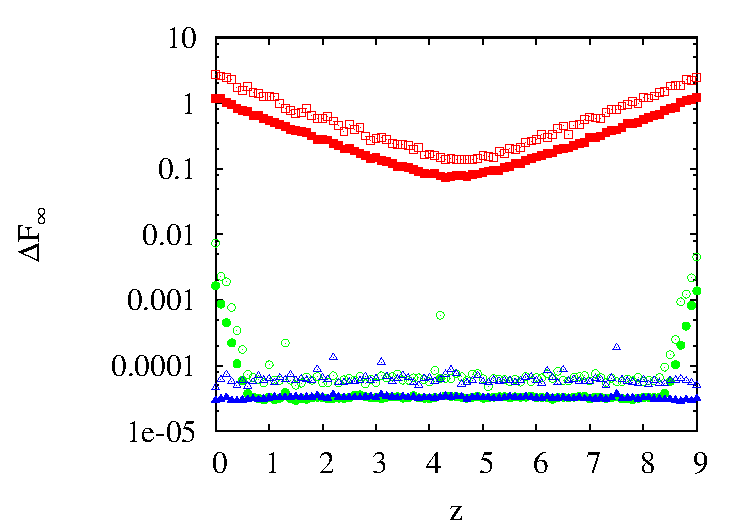
\includegraphics[width=0.4\textwidth]{figures/elc-errordist}
  \caption{Error distribution of the ELC method.}
  \label{fig:ELC-error}
\end{figure}

Figure \ref{fig:ELC-error} shows the error distribution of the ELC
method for a gap size of $10\%$ of the total system height. For MMM2D
and MMM1D the error distribution is less homogenous, however, also
here it is always better to have some extra precision, especially
since it is computationally cheap.


%%% Local Variables: 
%%% mode: latex
%%% TeX-master: "ug"
%%% End: 


\chapter{Maggs algorithm}
\label{chap:maggs}

\bibliographystyle{plainnat}
\bibliography{bibliography}

\printindex

\end{document}


%%% Local Variables: 
%%% mode: latex
%%% TeX-master: t
%%% End: 

%\listofcommands

%%% Local Variables: 
%%% mode: latex
%%% TeX-master: "ug"
%%% End: 


%%% Local Variables: 
%%% mode: latex
%%% TeX-master: "ug"
%%% End: 
